%% Master Thesis Template
%% Please update the specification through this link: https://daim.idi.ntnu.no/howto_thesis_submission.pdf

\documentclass[pdftex,10pt,b5paper,twoside]{book}
\usepackage[lmargin=25mm,rmargin=25mm,tmargin=27mm,bmargin=30mm]{geometry}

\usepackage{setspace}
\usepackage{graphicx}
\usepackage{amssymb}
\usepackage{mathrsfs}
\usepackage{amsthm}
\usepackage{amsmath}
\usepackage{color}
\usepackage[Rejne]{fncychap}
\usepackage[pdftex,bookmarks=true]{hyperref}
\usepackage[pdftex]{hyperref}
\hypersetup{
    colorlinks,%
    citecolor=black,%
    filecolor=black,%
    linkcolor=black,%
    urlcolor=black
}
\usepackage[font=small,labelfont=bf]{caption}
\usepackage{fancyhdr}
\usepackage{times}
\usepackage{float}
\restylefloat{figure}

% Setup references
\usepackage[backend=bibtex]{biblatex}
\addbibresource{bibfiles/bibtexlibs.bib}

\newcommand{\HRule}{\rule{\linewidth}{0.5mm}}

\renewcommand*\contentsname{Table of Contents}

\pagestyle{fancy}
\fancyhf{}
\renewcommand{\chaptermark}[1]{\markboth{\chaptername\ \thechapter.\ #1}{}}
\renewcommand{\sectionmark}[1]{\markright{\thesection\ #1}}
\renewcommand{\headrulewidth}{0.1ex}
\renewcommand{\footrulewidth}{0.1ex}
\fancypagestyle{plain}{\fancyhf{}\fancyfoot[LE,RO]{\thepage}\renewcommand{\headrulewidth}{0ex}}

\usepackage[caption=false,font=footnotesize]{subfig}

% My custom directives
%\usepackage{todonotes}

\newcommand{\cm}[1]{
    CITATION MISSING: #1
    %\todo[inline, color=cyan]{Citation missing: #1}
}

\newcommand{\todo}[1]{
    TODO: #1
}

\usepackage{tikz}

\usetikzlibrary{external}
\tikzexternalize[prefix=precompiled-figures/]

\usetikzlibrary{positioning}
\usetikzlibrary{shapes, arrows, fit, calc}
\tikzset{vertex/.style = {shape=circle,draw,minimum size=2em}}
\tikzset{edge/.style = {->, > = latex'}}
\tikzset{box/.style = {shape=rectangle,draw, minimum size=1.5cm}}

\usepackage{pgfplots}
\pgfplotsset{compat=newest}
\usepgfplotslibrary{statistics}

% #1=\addplots #2=scalefactor for ticks #3=Label
\newcommand{\myboxplot}[4]{
  \begin{tikzpicture}
    \pgfplotsset{
      boxplot/every box/.style={fill=gray},
      boxplot/every whisker/.style={fill=black, color=black},
      boxplot/box extend=0.7
    }
    \begin{axis}
      [
        axis x line=bottom,
        axis y line=left,
        xmin=-1,
        xmax=#4,
        ymin=0.4,
        ymax=1.05,
        ytick={0.4, 0.5, 0.6, 0.7, 0.8, 0.9, 1.0},
        scaled x ticks={real:#2},
        axis y discontinuity=crunch,
        xtick scale label code/.code={},
        boxplot/draw direction=y,
        xlabel=#3,
        ylabel=Accuarcy
      ]
      #1
    \end{axis}
  \end{tikzpicture}
}


% #1=table data #2=xlabel
\newcommand{\myscatterplot}[2]{
    \begin{tikzpicture}
        \begin{axis}
            [
                axis x line=bottom,
                axis y line=left,
                axis y discontinuity=crunch,
                ymin=0.3, ymax=1.1,
                ytick={0.3, 0.4, 0.5, 0.6, 0.7, 0.8, 0.9, 1.0},
                ylabel=Accuracy,
                xlabel=#2
            ]
            \addplot[scatter src=explicit, only marks, mark size=0.5pt]
            table {#1};
        \end{axis}
    \end{tikzpicture}
}

% #1=data #2=xlabel #3=ylabel
\newcommand{\myheatmap}[3]{
    \begin{tikzpicture}
        \begin{axis}
            [
                xlabel=#2,
                ylabel=#3,
                ymax=25,
                xmax=15,
                colormap/jet,
                colorbar,
                view={0}{90}
            ]
            \addplot3[surf, shader=flat]
            file {#1};
        \end{axis}
    \end{tikzpicture}
}


\begin{document}

\frontmatter

%% PART 1
%%The title page will be automatically generated and added by the DAIM system

%% PART 2
\section*{\Huge Abstract}
\addcontentsline{toc}{chapter}{Abstract}
$\\[0.5cm]$

\noindent Reservoir computing (RC), a relatively new approach to machine learning,
utilizes untrained recurrent neural networks as a reservoir of dynamics to preprocess some temporal task,
making it separable with a linear readout layer.
Potentially any sparsely connected network containing feedback loops can be a reservoir.
One such network is the random Boolean network (RBN),
which has previously been used in a reservoir computing setting.

Reservoir computing can be performed with physical or simulated reservoirs.
When using a physical reservoir for computation, as in evolution-in-materio,
one is often restricted in how one can perturb and read out the underlying substrate.
In this thesis, the following properties of RBN RC devices are investigated and related to physical reservoirs:
How task difficulty affects required reservoir size,
how much reservoir perturbation is optimal,
the performance of reservoir subsets,
and the relationship between an RBNs attractors and its performance as a reservoir.

Experiments confirm that the required reservoir size increases with the difficulty of the task at hand,
with the largest factor being how many bits of input the reservoir is required to remember.
Simulation of RBN RC systems can therefore aid in deciding the optimal size of physical reservoirs,
given a bridge between the computational power of the reservoir and RBNs can be deduced.
Optimal reservoir perturbation is found to lie at roughly 50\% of the size of the reservoir for RBNs with $K=3$.
When using smaller slices of a reservoir for computation,
lower amounts of total perturbation will be required as long as these perturbations are located within the same topological area.
Results also show that subsets of larger reservoirs will perform at least as well as a separate reservoir of equal size.
Any interference from the unused parts of the reservoir is either minimal or slightly positive.
Finally, no relationship is found between the attractors of a RBN and its performance in a RBN RC system.
It can therefore not be used for guiding the construction of accurate RBNs.

\cleardoublepage

\section*{\Huge Sammendrag}
\addcontentsline{toc}{chapter}{Sammendrag}
$\\[0.5cm]$

\noindent Reservoir computing (RC) er en relativt ny teknikk innen maskinlæring.
Et utrent rekurrent nevralt nettverk benyttes som et reservoar fyllt av dynamikk for å preprossesere et temporært problem,
og dermed gjøre det separerbart med et lineært avlesingslag.
Alle glissne nettverk med tilbakekoblinger kan potensielt benyttes som et reservoar.
Et slikt nettverk det tilfeldige Boolske nettverket (RBN),
som tidligere har blitt brukt i RC-systemer.

Reservoir computing kan benytte både fysiske og simulerte reservoar.
Når et fysisk reservoar brukes for beregning, som i evolution-in-materio,
har man ofte begrenset adgang til å påvirke samt lese ut verdier fra materialet.
I denne avhandlingen vil følgende egenskaper ved RBN RC-systemer bli undersøkt og relatert til fysiske reservoarer:
Hvordan kompleksiteten til oppgaven påvirker størrelsen på reservoaret,
hvor mye påvirkning som er optimalt,
hva ytelsen på subsett av større rerservoarer er,
og hva forbindelsen mellom et RBNs tiltrekkere og dets ytelse som reservoar er.

Våre eksperimenter bekrefter at den nødvendige størrelsen på reservoaret øker i takt med vanskelighetsgraden på oppgaven som skal løses.
Den største faktoren er hvor mange bits med input som må huskes.
Simuleringer av RBN RC-systemer kan derfor hjelpe i å avgjøre den optimale størrelsen på et fysisk reservoar,
gitt man finner en bro mellom målet for beregningskraft på det simulerte og fysiske reservoaret.
Optimal reservoarpåvirkning er funnet til å ligge på rundt 50\% av størrelsen på reservoaret (for RBN med konnektivitet 3).
Når man bruker et subsett av et reservoar for beregning så trengs det mindre mengder med påvirkning, gitt at påvirkingen skjer i samme del av reservoaret som leses av.
Våre resultater viser også at subsett av større reservoar yter like bra som separate reservoar av den størrelsen.
En eventuell interferens mellom den ubrukte delen av reservoaret og den brukte er enten neglisjerbar eller svakt positiv.
Det viste seg ingen sammenheng mellom tiltrekkerne til et RBN og dets ytelse i et RBN RC-system.
Dette kan dermed ikke brukes for å guide konstruksjonen av nøyaktige RBN.

\cleardoublepage


\section*{\Huge Acknowledgements}
\addcontentsline{toc}{chapter}{Acknowledgements}
$\\[0.5cm]$

\noindent I would like to thank my advisor Professor Gunnar Tufte for sharing his knowledge with me,
and guiding my research through this weird and awesome part of Computer Science.

Further, I would like to thank Porter Robinson for creating the album "Worlds",
which provided the soundtrack for my final week of writing.

\cleardoublepage


\tableofcontents
\addcontentsline{toc}{chapter}{Table of Contents}
\clearpage

\listoftables
\addcontentsline{toc}{chapter}{List of Tables}
\clearpage

\listoffigures
\addcontentsline{toc}{chapter}{List of Figures}
\clearpage

%\input{abbreviations.tex}	%% Optional

% Trenger ikke forklare hva alt er, men introduser begrepene
% Må ha evo-mamterio hva er introduksjon? Hvor mye stuff, mikroelektrodearray.
% Complex systems properties osv.
% Limited access to perturbation, ilmited access to information. Snapshot quantum mamterials.

\mainmatter
\chapter{Introduction}

Reservoir Computing (RC) is a category of machine learning that sprang out from the study of recurrent neural networks (RNNs).
In short, it utilizes the dynamics of some complex system dubbed a 'reservoir' to preprocess a time series problem,
transforming it from a temporal to a spacial one in the reservoir,
making it separable with a simple readout layer \cite{lukovsevivcius2012reservoir}.

Reservoir Computing can be used both with physical and theoretical reservoirs.
The original theoretical Echo State Networks \cite{jaeger2002adaptive} and Liquid State Machines \cite{natschlager2002liquid} provided the original basis for theoretical Reservoir Computing systems.
As alternative abstractions to RNNs,
both cellular automata \cite{yilmaz2014reservoir} and random Boolean networks \cite{rbn-reservoir} were introduced and successfully used in reservoir computing frameworks.
Random Boolean networks \cite{gershenson2004introduction} are an useful abstraction over many physical phenomena,
most famously used by Kauffman \cite{kauffman1969metabolic} as a model for the genetic regulatory network.
In the author's pre-thesis paper,
findings from \cite{rbn-reservoir} were reproduced and the reusability of trained readout layers investigated.
A neutrality in the state-space of possible RBNs was discovered.

Physical reservoirs take many shapes and forms.
In the ever-so-cited 'Pattern recognition in a bucket' paper \cite{fernando2003pattern},
the authors use a bucket of water to successfully perform speech recognition.
In \cite{farstad2015evolving},
a carbon nanotube based substrate is successfully used to evolve binary logic gates as well as stable Cellular Automata.
These can then be used to build a CA-based computing paradigm over this unconventional hardware.
As Cellular Automata are a special case of Random Boolean Networks,
any general findings about RBN RC systems may be applicable to RC systems using CAs.
The wider category of attempting to harness the power of unconventional physical devices for computation,
usually aided by artificial evolution,
is known as evolution-in-materio \cite{miller2002evolution}.

When using nontraditional physical devices for computation, as in evolution-in-materio,
one is often restricted in how one can perturb and read out the underlying substrate.
It might be prohibitively expensive or technologically infeasible to read the entire state of the reservoir,
and the values sampled might be affected by its neighborhood in unknown ways to us.
In \cite{demarse2005adaptive} the authors use living rat neurons in a microelectrode array to control an airplane in a flight simulator.
Only subsets of the computational substrate are used,
and the neuronal connections even change over time.
In addition, the microelectrode array presents a limited resolution view of the computational substrate.
Questions include how the unused parts of the reservoir impact the parts used for computation,
and how large the reservoir actually needs to be to solve the task at hand.

It has been shown that Reservoir Computing using Random Boolean Networks is a feasible approach to solving binary time-series problems,
as well as being a potentially useful abstraction over physical Reservoir Computing devices.
In this thesis, the properties of these RRC systems are further investigated,
with the motivation of using the results as a template for instrumenting and performing computations on physical Reservoir Computing systems.

The following questions will be answered in this thesis:
\begin{enumerate}
    \item How small can a RRC system be while still solving its task at $ \geq 98\% $ accuracy?
    \item Does the optimal amount of reservoir perturbation depend on the task at hand?
    \item Does one have to read the state of the entire reservoir to maintain task accuracy?
    \item Is there a correlation between the topological characteristics of the RBN (number of attractors, attractor length) and its performance as a reservoir?
\end{enumerate}

Questions two and three are of specific interest to the implementation of physical reservoirs and evolution-in-materio devices.
What these approaches have in common is that physical substrates,
with varying degrees of perturbation ability and insight into the internal state,
are used for computation.
Their couplings to theoretical frameworks such as Reservoir Computing motivate the exploration of the effects of limited perturbation and readout possibilities on reservoir performance.

\section{Thesis structure}

The thesis is structured as follows:
Chapter \ref{chapter:background} provides background information on reservoir computing, random Boolean networks, evolution-in-materio, and using RBNs for Reservoir Computing.
Chapter \ref{chapter:methodology} describes the experimental setup and methodology used for performing experiments.
Chapter \ref{chapter:experiments} contains an in-depth descriptions of each experiment,
the results obtained, and a discussion thereof.
Chapter \ref{chapter:conclusion} concludes the thesis and mentions further work.


\chapter{Background}
\label{chapter:background}

\section{A Brief Introduction to Reservoir Computing}
\label{section:reservoir-computing-introduction}

Recurrent Neural Networks (RNNs), as opposed to feed-forward neural networks,
are notoriously time consuming and difficult to train \cite{Schrauwen2007}.
This is due to feedback from the recurrent connections during the training process,
allowing small topology changes to drastically change a network's position in the fitness landscape.

It was therefore proposed in both \cite{jaeger2002adaptive} (as Echo State Networks, or ESN)
and \cite{natschlager2002liquid} (as Liquid State Machines, or LSM) to separate the RNN into two parts,
the untrained reccurrent reservoir, and the trained readout layer.
Both of these methods have been unified into the field of Reservoir Computing,
now focusing on the separate training and evolution of the recurrent and readout parts \cite{lukovsevivcius2012reservoir}.
Exiting applications of Reservoir Computing include speech and handwriting recognition,
as well as controlling robotics \cite{lukovsevivcius2012reservoir}.

\begin{figure}[ht]
    \caption{
        Schematic of a general Reservoir Computing system containing adjustable biases, feedback loops, reservoir and readout layers,
        which are described in section \ref{section:reservoir-computing-introduction}.
        Inspired by figures from \cite{Schrauwen2007} and \cite{Jaeger:2007}.
    }
    \label{fig:rc-schema}
    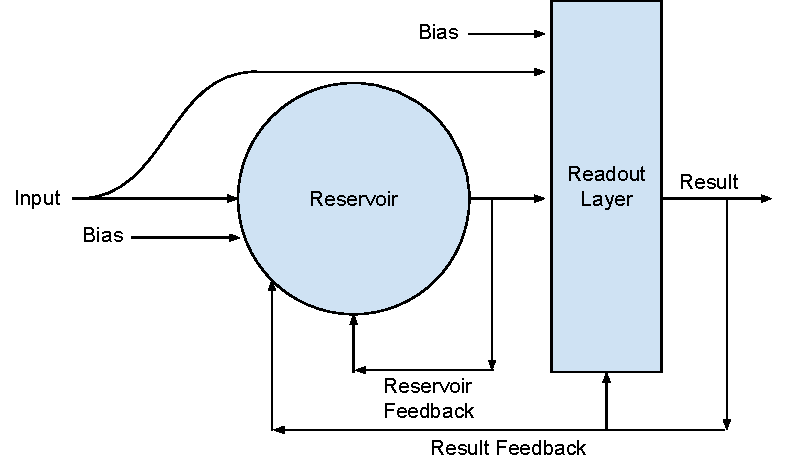
\includegraphics[width=\columnwidth]{background/reservoir_computing_schema.pdf}
\end{figure}

A generalized structure of a Reservoir Computing system with all bells and whistles is shown in figure \ref{fig:rc-schema}.
The main components are the reservoir and the readout layer.
At each timestep in the core model,
the reservoir receives the current input signal as well as its previous state (it is recurrent after all).
It transforms it, and passes it on to the readout layer.
The output layer frequently receives the teacher input as well.
The internal weights of the reservoir are usually randomized and left untrained,
with the weights of the readout layer being adjusted by some learning algorithm.
This can be linear or ridge regression for offline learning,
or recursive least sqares for online learning \cite{Schrauwen2007}.

There are many extensions to the base model.
The reservoir and output layers can receive biases:
The readout bias is used for regularizing the reservoir state in case the problem is ill-posed,
but isn't needed when using a model like ridge regression, which performs regularization internally \cite{Schrauwen2007}.
Reservoir bias is used for stabilizing models which feeds the output layer back into the reservoir,
which may be needed if the problem entails producing oscillating output \cite{Jaeger:2007}.
Teacher forcing,
that is forcing the states of the output layer to those expected by the trainer for the first n timesteps,
usually speed up the convergence of the learning method used,
and may in some cases be required to at all achieve stability \cite{jaeger2002tutorial}.

For a deeper dive into Reservoir Computing,
consult papers \cite{Schrauwen2007}, \cite{lukovsevivcius2012reservoir}, and \cite{Jaeger:2007}.

\section{Alternatives to Classical Reservoirs}

Are there other types of complex systems that can be used as reservoirs?
What properties must these reservoirs have to be able to solve problems?

Complex networks similar to the sparsely connected RNNs used  ESN and LSM systems include Cellular Automata \cite{wolfram2002new} and Random Boolean Networks \cite{kauffman1969metabolic}.
Cellular Automata are regular grids of cells containing some state,
each cell connected to its neighbors in the grid.
Cells then update in lockstep according to some shared transition table,
creating a new generation.
RBNs can be seen upon as an abstraction over CAs again,
allowing for nonlocal neighbors and variable updating rules.
They will be introduced in depth in section \ref{section:rbns}.

Both CAs and RBNs have successfully been used in Reservoir Computing systems \cite{yilmaz2014reservoir} \cite{rbn-reservoir}.
Both models are simple, and can be implemented in software,
hardware (FPGAs), and in materio \cite{miller2002evolution} \cite{farstad2015evolving}.

This computational paradigm is known as Cellular Computing,
and provides a potentially powerful alternative to classical computers,
leveraging extreme parallelism, simple components and local state \cite{sipper1999emergence}.

\section{A Brief Introduction to Boolean Networks}
\label{section:rbns}

Random Boolean Networks, also known as Kaffman networks,
were originally developed as a model of gene regulatory networks \cite{kauffman1969metabolic},
the complex system that regulates how genes in multicellular organisms interact with each other.
The model requires no assumptions about the inner workings of the actual nodes,
which allows it to model phenomena where the exact internal workings of the system may be unknown.

The simplification of a system to a boolean model doesn't pose a problem,
as any multi-valued network can be transformed to a corresponding binary one.

A RBN is usually described by its number of nodes $N$ and the in-degree $K$ of the nodes,
that is, how many nodes each node depends on (also known as its ancestors).
RBNs can have both homogenous and heterogenous in-degrees.
In heterogenous networks, one usually describes the average connectivity $\langle K \rangle$ instead.

Each node can have a state of zero or one.
The next state of the node is solely determined by the current combination of states of its ancestors.
Each combination leads to a new state of zero or one,
with the probability given by a binomial distribution usually having $\langle P \rangle = 0.5$.
Figure \ref{figure:sample-homogenous-rbn} visualizes a homogenous RBN with $N=3, K=2, P=0.5$.

\begin{figure}
  \centering
  \subfloat[RBN topology]{
    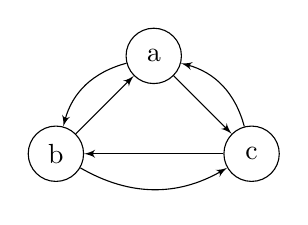
\begin{tikzpicture}[node distance = 5em]
      \node[vertex] (a) {a};
      \node[vertex] (b) [below left of=a] {b};
      \node[vertex] (c) [below right of=a] {c};

      \draw[edge] (a) to[bend right] (b);
      \draw[edge] (a) to (c);

      \draw[edge] (b) to (a);
      \draw[edge] (b) to[bend right] (c);

      \draw[edge] (c) to[bend right] (a);
      \draw[edge] (c) to (b);
    \end{tikzpicture}
  }
  \subfloat[Transition table for node a]{
    \begin{tabular}[b]{ c c | c}
      \multicolumn{2}{c}{Ancestor states} & New state \\
      \hline
      0 & 0 & 0 \\
      0 & 1 & 1 \\
      1 & 0 & 0 \\
      1 & 1 & 1 \\
    \end{tabular}
  }
  \caption{An example homogenous RBN with $N=3, K=2, P=0.5$.}
  \label{figure:sample-homogenous-rbn}
\end{figure}

In the simplest RBN updating scheme, all nodes update in lockstep.
This is known as the Classical RBN updating scheme (CRBN).
The states of the RBN at the next timestep $t+1$ therefore only depend on the states at the previous timestep $t$.
As the number of RBN states is finite ($2^{n\_nodes}$),
the system will eventually revisit a previously visited state.
This set of repeating states is known as an \emph{attractor},
and a deterministic system cannot escape from it.
If the attractor consists of a single state it is known as a point attractor,
otherwise a cycle attractor.
The set of states leading towards an attractor is known as its \emph{basin of attraction}.
A cycle attractor can be observed in figure \ref{figure:rbn-critical},
while a point attractor is observed in figure \ref{figure:rbn-ordered}.

A criticism of the classical model is that gene regulation networks are updating continiously,
as opposed to in lockstep \cite{gershenson2004introduction}.
There are therefore a number of alternate updating schemes which can be categorized by whether they are deterministic or nondeterministic, as well as synchronous and asynchronous.

The dynamics of an RBN can be categorized as being in either the ordered, critical, or chaotic phase.
These phases can be identified by how large a part of the network state is able to change over time,
whether similar states tend to converge or diverge over time,
and the networks resistance to perturbations (outside changes to the network).

One way to obtain these phases analytically is by comparing the resulting states of two identical RBNs where one is subject to some perturbation \cite{gershenson2004introduction}.
For visual identification, we plot the states of the RBN in a square lattice,
with the network states plotted horizontally, and time flowing downwards.
A node is drawn as white if its state is one, black otherwise.
The phases are visualized in Figure \ref{figure:rbn-phases}.

\begin{figure}
  \subfloat[Ordered phase, K=1]{
    
\includegraphics[width=0.3\columnwidth]{background/ordered-phase.pdf}
    \label{figure:rbn-ordered}
  }
  \subfloat[Critical phase, K=2]{
    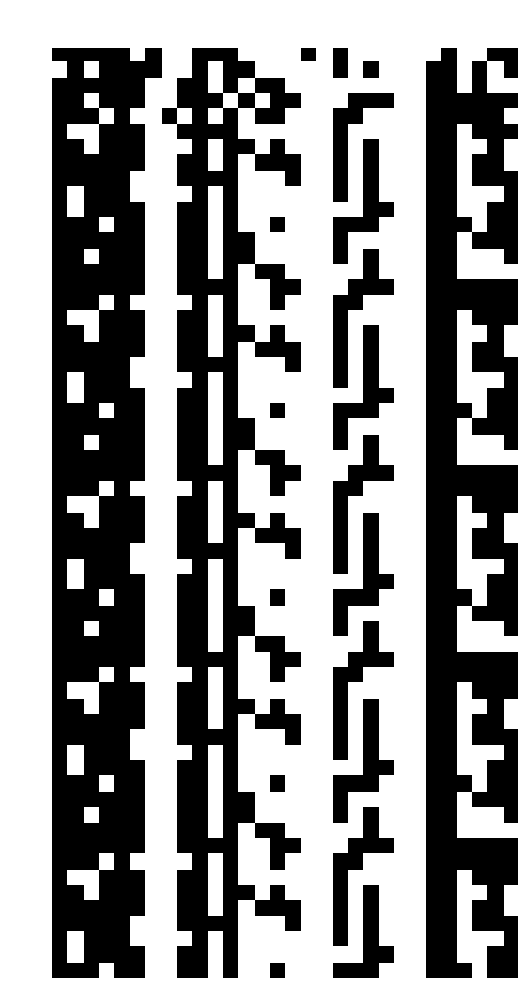
\includegraphics[width=0.3\columnwidth]{background/critical-phase.pdf}
    \label{figure:rbn-critical}
  }
  \subfloat[Chaotic phase, K=3]{
    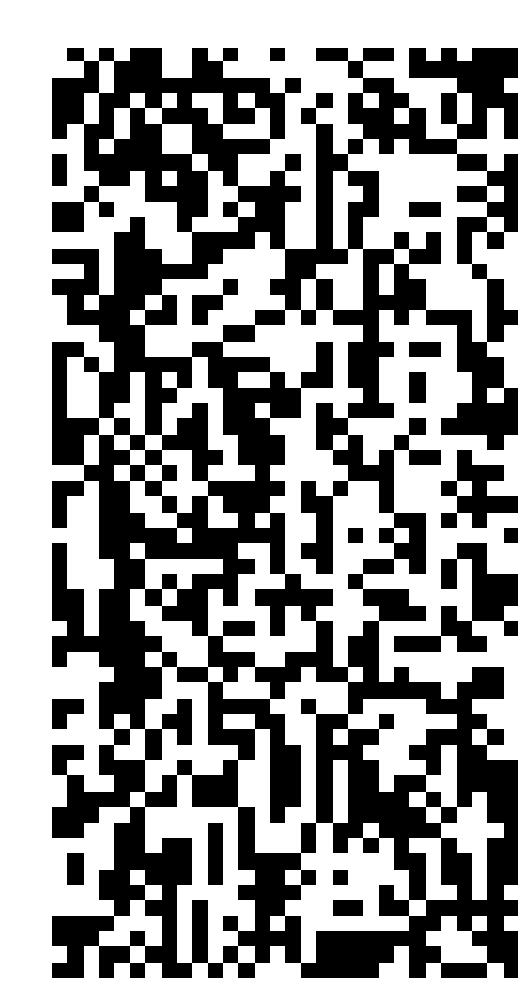
\includegraphics[width=0.3\columnwidth]{background/chaotic-phase.pdf}
    \label{figure:rbn-chaotic}
  }

  \caption{
    Trajectories through state-space for RBNs with $N=30, K=[1,2,3]$, visualizing the different phases.
    Time flows downwards the lattice, while RBN states are shown along the X-axis.
    with the network states plotted horizontally, and time flowing downwards.
    Images created with the developed RBN-simulator.
  }
  \label{figure:rbn-phases}
\end{figure}

In general, RBNs in the critical phase are the most interesting.
These are seemingly able to support information transmission, storage and modification,
all capacities required for computation \cite{langton3computation}.
Critical systems are found on the edge of chaos,
on the phase transition between ordered and chaotic networks \cite{gershenson2004introduction}.
For RBNs with $\langle p \rangle = 0.5$,
critical dynamics are usually found at $\langle K \rangle = 2$ \cite{gershenson2004introduction},
although one could still find networks with such dynamics for different values of $\langle K \rangle$.

A thorough introduction to the field of RBNs is available in \cite{gershenson2004introduction}.

\section{RBN Reservoir systems}
\label{subsection:rbn-reservoir-systems}

How does one adapt a RBN for use as a reservoir in a RBN-RC device?
RBNs aren't usually designed to take external input.
We do however, have the concept of perturbation,
the external flipping of bits in the network's state,
transition tables or edges.
This can be utilized to create RBNs that take input,
by continiously perturbing the RBN nodes by the bits of the input sequence.

Questions that follow are how many bits should the network consume at a time,
how many of the network nodes should be perturbed by the input at each timestep,
and what dynamics must such a reservoir have to allow for the computation of interesting problems?

\subsection{A working system}

In \cite{rbn-reservoir} functioning RBN-RC systems are created and analyzed.
These RBN-RC systems have heterogenous connectivity,
consume one bit of input at each timestep ($I=1$),
perturbing $IC$ of the $N$ nodes in the process.
The readout layer can be any node performing some kind of regression of the reservoir state against expected outout for the current task, e.g. linear regression.
Such a setup is shown in Figure \ref{figure:rbn-reservoir}.

\begin{figure}
  \centering
  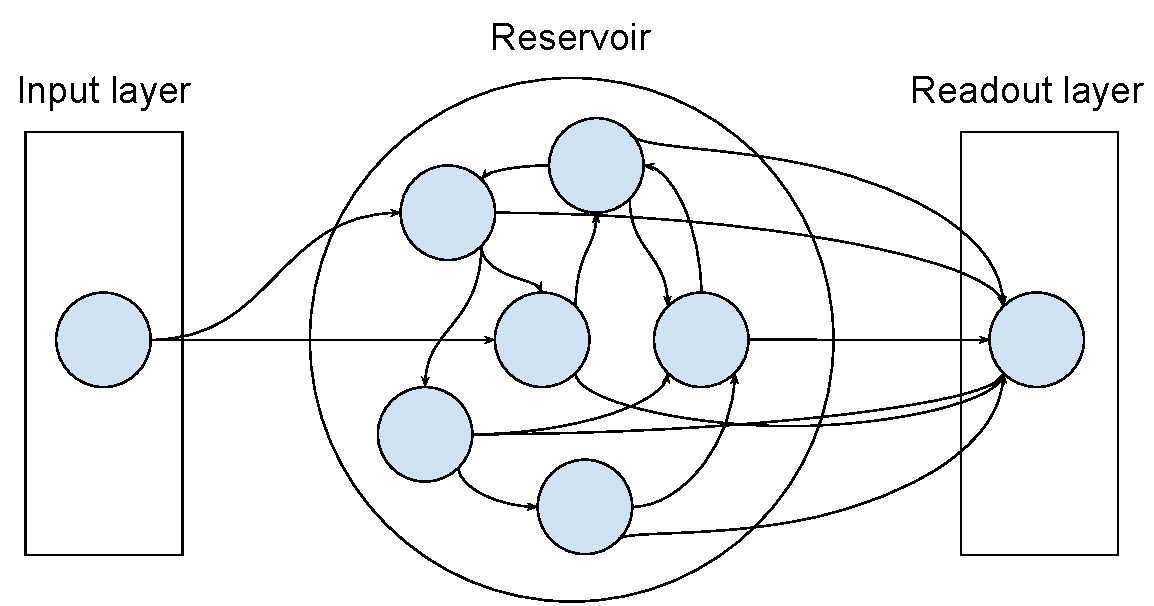
\includegraphics[width=\columnwidth]{background/RBN-Reservoir.pdf}
  \caption{
    RBN-Reservoir system with $I=1, IC=2, K=2, N=6$ with the entire reservoir sate used for regression.
    The reservoir transforms the problem from a temporal one to a multidimentional spatial one.
    The readout layer the performs some kind of learning on the reservoir states against the expected output for the current task.}
  \label{figure:rbn-reservoir}
\end{figure}

\subsection{Tasks}
\label{section:tasks}

To measure the real-life performance and accuracy of the RBN Reservoir systems,
two tasks are introduced: Temporal Density and Temporal Parity \cite{rbn-reservoir}.
Both require the reservoir to be able to retain information for a sliding window of size $ n $,
offset by some value $ t $, back through the input stream.
The Temporal Parity task requires us to determine if there were an odd number of ones in the sliding window,
the Temporal Density task to determine whether there were a majority of ones.
The Former is visualized in figure \ref{figure:temporal-parity}.

Both tasks will be used to benchmark the reservoirs created later in this paper.

\begin{figure}
  \subfloat[Input]{
    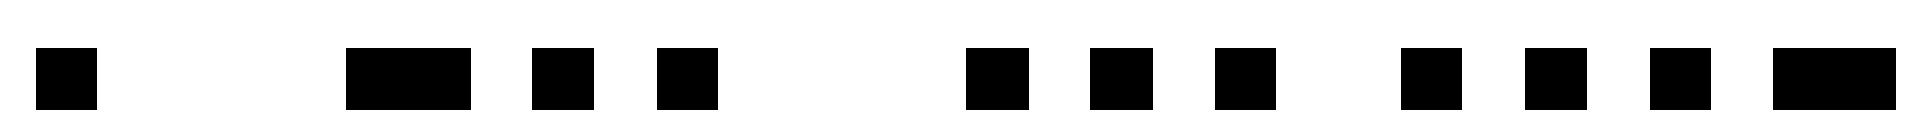
\includegraphics[width=\columnwidth]{background/temporal_parity-10-200-3-input.pdf}
  }

  \subfloat[Correct output]{
    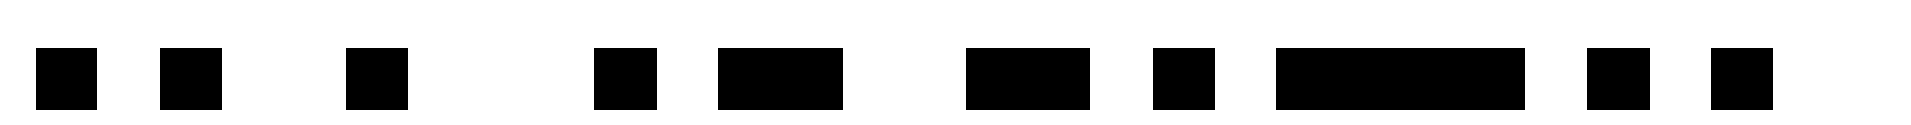
\includegraphics[width=\columnwidth]{background/temporal_parity-10-200-3-output.pdf}
  }

  \caption{
    The first 30 elements of a Temporal Parity task with $[n=3, t=0]$.
    A one is visualized as white, while a zero is black.
    We see that correct output at time $i$ is equal to there being an odd number of $1$s in inputs $[i, i-1, i-2]$
  }
  \label{figure:temporal-parity}
\end{figure}

\subsection{Computational capability}
\label{section:computational-capability}
For an RBN-reservoir to perform well at computational tasks,
it must be able to both forget past perturbations and keep two input streams that have begun converging separated \cite{bertschinger2004real}.

These two properties are coined \textit{fading memory} and \textit{separation property},
and can be measured \cite{rbn-reservoir} as follows.

Create two equal input streams \#1 and \#2 of length $T$.
If measuring \textit{fading memory}, flip the first bit in stream \#2.
If measuring \textit{separation property}, flip all bits up to bit $T-t$ in stream \#2
($t$ being the required depth of separation).
For both input streams, reset reservoir state, perturb the reservoir with the input stream,
and store the final state.
The score of the measure is then defined as the normalized hamming distance between the resulting states.
The computational capability $\Delta$ of an RBN-reservoir is then defined as
\begin{equation}
  \Delta_{Tt} = separation\_property_{Tt} - fading\_memory_{T}
\label{formula:accuracy}
\end{equation}
Analyzing different RBN-reservoirs with this metric \cite{rbn-reservoir},
a high $\Delta$ is found to correlate with critical connectivity ($\langle K \rangle = 2$).
For all RBN-reservoirs, $\Delta$ drops when increasing the required separation $t$,
and is maximized when one doesn't have to remember anything at all ($t=0$).

\subsection{Optimal perturbance}
\label{section:optimal-perturbance}
It is found that the optimal amount of reservoir perturbance,
adjustable by the number of connections between the input layer and the reservoir,
depends on both the task size, how many steps in time are required to be remembered,
and the dynamics of the reservoir.
\textit{Chaotic reservoirs} require few input connections to be able to properly spread information,
but perform poorly on larger tasks due to past perturbations still floating around the reservoir.
\textit{Ordered reservoirs} quickly forget past perturbations, allowing some success for larger tasks,
but their inability to remember past perturbations renders them useless for many tasks.
\textit{Critical reservoirs} require connectivity somewhere in the middle.
Able to forget as well as remember, they perform accurately independent of task size.


\section{Evo Materio, water bucket}
\todo{Gotta write about Evo Materio. I'm a bit unsure where to put this section in the background chapter,
and what angle it should have-if any- that's different from just showing some physical reservoir systems}

The 'Water bucket' paper investigated the use of an actual bucket of water as a reservoir \cite{fernando2003pattern},
successfully recognizing patterns and achieving decent performance at that.
The RBN Reservoir approach has also been found to be viable \cite{rbn-reservoir} .


\section{Viability of RBNs for Reservoir Computing}
\label{section:pre-thesis-project}

In the authors pre-thesis paper, the dynamics, performance, and viability of RBNs used for Reservoir Computing (RRC) was investigated.
A functioning RBN Reservoir Computing system was implemented,
and its results validated against and found in accordance with those from \cite{rbn-reservoir}.
This self-written framework serves as the basis for the simulations and analysis perfored in this thesis as well.

A positive correlation between the computational capability (section \ref{section:computational-capability}) of a reservoir and its actual performance is found.
The optimal connectivity for homogenous reservoirs is found to be $K=3$ as opposed to $\langle K \rangle = 2$ for heterogenous reservoirs \cite{rbn-reservoir}.
Finally, the required input connectivity is found to rise with the presence of chaotic dynamics in the reservoir.
The figures backing this conclusion are shown in \ref{figure:results:temporal-parity-3} and \ref{figure:results:temporal-parity-5}.

Finally, a one-to-many mapping between the readout layer in an already-trained RRC system and different RBN reservoirs was found,
with there being a seemingly large set of interchangeable reservoirs for each readout layer.
This makes the potential use of a smaller generative genome for evolving RRC systems interesting.
Even though it hits fewer points in the RBN fitness landscape than the fixed genome used in this paper,
a large amount of these points are still usable for each instance of a working readout layer.

\begin{table}[ht]
    \centering
    \caption{Task parameters for the pre-thesis project.}
    \label{table:pre-thesis-tasks}
    \begin{tabular}{ll}
        \hline
        \textbf{Parameter} & \textbf{Configuration} \\
        \hline
        \hline
        Task type               & Temporal Parity \\
        Training dataset length & 4 000                       \\
        Test dataset length     & 200                         \\
        $N$ (window size)       & 3 and 5                     \\
        $t$ (offset)            & 0 \\
        \hline
    \end{tabular}
\end{table}

\begin{figure*}[!t]
    \centering
    \caption{
        Plots for Temporal Parity with $N=3$ (parameters in table \ref{section:tasks}).
        Figures \ref{fig:res:d-100-3-1}--\ref{fig:res:d-100-3-3} plot the accuracies of the sampled RBNs against their input connectivity,
        for K=1–3 respectively.
        Figures \ref{fig:res:c-100-3-1}--\ref{fig:res:c-100-3-3} plot the accuracy of the previous figures against their Computational Capability ($T=100, t=3$).
    }
    \label{figure:results:temporal-parity-3}
    \resizebox{\textwidth}{!}{
        \subfloat[K=1]{
            \label{fig:res:d-100-3-1}
            \myboxplot{
% L: 0
\addplot[mark=*,boxplot, boxplot/draw position=0]
table[row sep=\\, y index=0] {
data
0.52 \\
0.52 \\
0.48 \\
0.52 \\
0.52 \\
0.48 \\
0.52 \\
0.52 \\
0.52 \\
0.52 \\
0.47 \\
0.52 \\
0.56 \\
0.52 \\
0.47 \\
0.52 \\
0.52 \\
0.52 \\
0.52 \\
0.52 \\
0.47 \\
0.52 \\
0.48 \\
0.47 \\
0.52 \\
0.43 \\
0.52 \\
0.52 \\
0.47 \\
0.52 \\
};
% L: 1
\addplot[mark=*,boxplot, boxplot/draw position=1]
table[row sep=\\, y index=0] {
data
0.55 \\
0.465 \\
0.47 \\
0.36 \\
0.48 \\
0.465 \\
0.47 \\
0.425 \\
0.47 \\
0.455 \\
0.485 \\
0.475 \\
0.48 \\
0.44 \\
0.465 \\
0.645 \\
0.47 \\
0.48 \\
0.36 \\
0.48 \\
0.36 \\
0.48 \\
0.48 \\
0.465 \\
0.52 \\
0.48 \\
0.495 \\
0.48 \\
0.36 \\
0.475 \\
};
% L: 2
\addplot[mark=*,boxplot, boxplot/draw position=2]
table[row sep=\\, y index=0] {
data
0.465 \\
0.465 \\
0.47 \\
0.36 \\
0.36 \\
0.475 \\
0.48 \\
0.49 \\
0.51 \\
0.48 \\
0.475 \\
0.465 \\
0.465 \\
0.47 \\
0.475 \\
0.465 \\
0.475 \\
0.515 \\
0.48 \\
0.475 \\
0.465 \\
0.465 \\
0.475 \\
0.455 \\
0.455 \\
0.48 \\
0.48 \\
0.475 \\
0.47 \\
0.49 \\
};
% L: 3
\addplot[mark=*,boxplot, boxplot/draw position=3]
table[row sep=\\, y index=0] {
data
0.41 \\
0.47 \\
0.405 \\
0.405 \\
0.54 \\
0.475 \\
0.48 \\
0.5 \\
0.5 \\
0.48 \\
0.4 \\
0.45 \\
0.425 \\
0.485 \\
0.465 \\
0.445 \\
0.355 \\
0.465 \\
0.47 \\
0.475 \\
0.595 \\
0.485 \\
0.525 \\
0.61 \\
0.475 \\
0.645 \\
0.36 \\
0.475 \\
0.49 \\
0.465 \\
};
% L: 4
\addplot[mark=*,boxplot, boxplot/draw position=4]
table[row sep=\\, y index=0] {
data
0.465 \\
0.585 \\
0.645 \\
0.405 \\
0.475 \\
0.465 \\
0.485 \\
0.36 \\
0.465 \\
0.48 \\
0.475 \\
0.545 \\
0.465 \\
0.41 \\
0.485 \\
0.475 \\
0.47 \\
0.465 \\
0.595 \\
0.465 \\
0.41 \\
0.47 \\
0.47 \\
0.495 \\
0.485 \\
0.49 \\
0.465 \\
0.475 \\
0.48 \\
0.48 \\
};
% L: 5
\addplot[mark=*,boxplot, boxplot/draw position=5]
table[row sep=\\, y index=0] {
data
0.465 \\
0.465 \\
0.465 \\
0.57 \\
0.36 \\
0.475 \\
0.465 \\
0.475 \\
0.435 \\
0.475 \\
0.53 \\
0.465 \\
0.48 \\
0.355 \\
0.555 \\
0.47 \\
0.475 \\
0.455 \\
0.465 \\
0.475 \\
0.475 \\
0.475 \\
0.475 \\
0.52 \\
0.425 \\
0.585 \\
0.465 \\
0.465 \\
0.405 \\
0.485 \\
};
% L: 6
\addplot[mark=*,boxplot, boxplot/draw position=6]
table[row sep=\\, y index=0] {
data
0.465 \\
0.54 \\
0.54 \\
0.47 \\
0.475 \\
0.435 \\
0.475 \\
0.405 \\
0.355 \\
0.465 \\
0.465 \\
0.465 \\
0.465 \\
0.47 \\
0.41 \\
0.465 \\
0.465 \\
0.465 \\
0.475 \\
0.475 \\
0.465 \\
0.46 \\
0.645 \\
0.465 \\
0.465 \\
0.475 \\
0.475 \\
0.475 \\
0.465 \\
};
% L: 7
\addplot[mark=*,boxplot, boxplot/draw position=7]
table[row sep=\\, y index=0] {
data
0.465 \\
0.465 \\
0.475 \\
0.645 \\
0.475 \\
0.475 \\
0.465 \\
0.465 \\
0.48 \\
0.465 \\
0.475 \\
0.465 \\
0.395 \\
0.465 \\
0.475 \\
0.465 \\
0.645 \\
0.465 \\
0.475 \\
0.47 \\
0.48 \\
0.475 \\
0.47 \\
0.425 \\
0.475 \\
0.465 \\
0.465 \\
0.475 \\
0.47 \\
0.465 \\
};
% L: 8
\addplot[mark=*,boxplot, boxplot/draw position=8]
table[row sep=\\, y index=0] {
data
0.465 \\
0.465 \\
0.465 \\
0.465 \\
0.465 \\
0.475 \\
0.465 \\
0.465 \\
0.465 \\
0.465 \\
0.475 \\
0.465 \\
0.475 \\
0.465 \\
0.465 \\
0.48 \\
0.465 \\
0.465 \\
0.475 \\
0.465 \\
0.47 \\
0.475 \\
0.465 \\
0.475 \\
0.465 \\
0.465 \\
0.465 \\
0.475 \\
0.465 \\
0.475 \\
};
% L: 9
\addplot[mark=*,boxplot, boxplot/draw position=9]
table[row sep=\\, y index=0] {
data
0.475 \\
0.465 \\
0.475 \\
0.36 \\
0.465 \\
0.535 \\
0.465 \\
0.465 \\
0.535 \\
0.475 \\
0.465 \\
0.595 \\
0.475 \\
0.465 \\
0.475 \\
0.475 \\
0.465 \\
0.475 \\
0.475 \\
0.475 \\
0.465 \\
0.465 \\
0.475 \\
0.475 \\
0.475 \\
0.475 \\
0.465 \\
0.535 \\
0.475 \\
0.535 \\
};
% L: 10
\addplot[mark=*,boxplot, boxplot/draw position=10]
table[row sep=\\, y index=0] {
data
0.535 \\
0.535 \\
0.535 \\
0.535 \\
0.535 \\
0.535 \\
0.535 \\
0.535 \\
0.535 \\
0.535 \\
0.535 \\
0.535 \\
0.535 \\
0.535 \\
0.535 \\
0.535 \\
0.535 \\
0.535 \\
0.535 \\
0.535 \\
0.535 \\
0.535 \\
0.535 \\
0.535 \\
0.535 \\
0.535 \\
0.535 \\
0.535 \\
0.535 \\
0.535 \\
};
}{0.1}{Input Connectivity}{10}

        }
        \subfloat[K=1]{
            \label{fig:res:c-100-3-1}
            \myscatterplot{background/pre-project/computational-power-100-3-1.dat}
        }
    }

    \resizebox{\textwidth}{!}{
        \subfloat[K=2]{
            \label{fig:res:d-100-3-2}
            \myboxplot{
% L: 0
\addplot[mark=*, mark=*,boxplot, boxplot/draw position=0]
table[row sep=\\, y index=0] {
data
0.545 \\
0.59 \\
0.465 \\
0.465 \\
0.515 \\
0.515 \\
0.515 \\
0.465 \\
0.515 \\
0.515 \\
0.515 \\
0.465 \\
0.59 \\
0.515 \\
0.525 \\
0.515 \\
0.465 \\
0.515 \\
0.545 \\
0.465 \\
0.515 \\
0.56 \\
0.515 \\
0.525 \\
0.465 \\
0.525 \\
0.565 \\
0.515 \\
0.515 \\
0.515 \\
};
% L: 1
\addplot[mark=*, mark=*,boxplot, boxplot/draw position=1]
table[row sep=\\, y index=0] {
data
0.595 \\
0.605 \\
0.99 \\
0.635 \\
0.99 \\
0.57 \\
0.525 \\
0.605 \\
0.99 \\
0.515 \\
0.58 \\
0.58 \\
0.57 \\
0.58 \\
0.755 \\
0.57 \\
0.605 \\
0.535 \\
0.585 \\
0.545 \\
0.565 \\
0.62 \\
0.6 \\
0.585 \\
0.57 \\
0.62 \\
0.515 \\
0.58 \\
0.885 \\
0.57 \\
};
% L: 2
\addplot[mark=*, mark=*,boxplot, boxplot/draw position=2]
table[row sep=\\, y index=0] {
data
0.55 \\
0.555 \\
0.99 \\
0.585 \\
0.84 \\
0.54 \\
0.6 \\
0.99 \\
0.535 \\
0.99 \\
0.935 \\
0.56 \\
0.825 \\
0.555 \\
0.59 \\
0.535 \\
0.55 \\
0.565 \\
0.815 \\
0.99 \\
0.545 \\
0.99 \\
0.56 \\
0.625 \\
0.83 \\
0.99 \\
0.58 \\
0.935 \\
0.57 \\
0.53 \\
};
% L: 3
\addplot[mark=*, mark=*,boxplot, boxplot/draw position=3]
table[row sep=\\, y index=0] {
data
0.99 \\
0.99 \\
0.935 \\
0.61 \\
0.99 \\
0.99 \\
0.99 \\
0.97 \\
0.99 \\
0.71 \\
0.72 \\
0.635 \\
0.625 \\
0.99 \\
0.905 \\
0.57 \\
0.845 \\
0.73 \\
0.99 \\
0.99 \\
0.99 \\
0.89 \\
0.99 \\
0.97 \\
0.855 \\
0.99 \\
0.975 \\
0.99 \\
0.99 \\
0.99 \\
};
% L: 4
\addplot[mark=*, mark=*,boxplot, boxplot/draw position=4]
table[row sep=\\, y index=0] {
data
0.99 \\
0.99 \\
0.955 \\
0.945 \\
0.99 \\
0.59 \\
0.99 \\
0.99 \\
0.99 \\
0.775 \\
0.99 \\
0.585 \\
0.99 \\
0.99 \\
0.99 \\
0.99 \\
0.835 \\
0.99 \\
0.99 \\
0.99 \\
0.49 \\
0.99 \\
0.99 \\
0.845 \\
0.99 \\
0.985 \\
0.535 \\
0.99 \\
0.955 \\
0.99 \\
};
% L: 5
\addplot[mark=*, mark=*,boxplot, boxplot/draw position=5]
table[row sep=\\, y index=0] {
data
0.99 \\
0.99 \\
0.99 \\
0.99 \\
0.99 \\
0.8 \\
0.99 \\
0.99 \\
0.99 \\
0.98 \\
0.99 \\
0.98 \\
0.99 \\
0.99 \\
0.99 \\
0.61 \\
0.99 \\
0.535 \\
0.99 \\
0.99 \\
0.53 \\
0.99 \\
0.52 \\
0.99 \\
0.735 \\
0.99 \\
0.665 \\
0.99 \\
0.99 \\
0.99 \\
};
% L: 6
\addplot[mark=*, mark=*,boxplot, boxplot/draw position=6]
table[row sep=\\, y index=0] {
data
0.62 \\
0.595 \\
0.99 \\
0.99 \\
0.85 \\
0.99 \\
0.99 \\
0.855 \\
0.97 \\
0.635 \\
0.99 \\
0.99 \\
0.545 \\
0.97 \\
0.99 \\
0.99 \\
0.99 \\
0.99 \\
0.99 \\
0.99 \\
0.96 \\
0.99 \\
0.99 \\
0.99 \\
0.99 \\
0.895 \\
0.99 \\
0.71 \\
0.99 \\
0.84 \\
};
% L: 7
\addplot[mark=*, mark=*,boxplot, boxplot/draw position=7]
table[row sep=\\, y index=0] {
data
0.99 \\
0.99 \\
0.99 \\
0.955 \\
0.635 \\
0.52 \\
0.99 \\
0.605 \\
0.95 \\
0.905 \\
0.715 \\
0.99 \\
0.99 \\
0.965 \\
0.585 \\
0.99 \\
0.745 \\
0.96 \\
0.81 \\
0.99 \\
0.505 \\
0.91 \\
0.635 \\
0.99 \\
0.99 \\
0.99 \\
0.99 \\
0.99 \\
};
% L: 8
\addplot[mark=*, mark=*,boxplot, boxplot/draw position=8]
table[row sep=\\, y index=0] {
data
0.84 \\
0.84 \\
0.865 \\
0.525 \\
0.97 \\
0.525 \\
0.93 \\
0.635 \\
0.94 \\
0.525 \\
0.99 \\
0.635 \\
0.525 \\
0.675 \\
0.99 \\
0.715 \\
0.715 \\
0.635 \\
0.675 \\
0.525 \\
0.865 \\
0.785 \\
0.99 \\
0.99 \\
0.99 \\
0.99 \\
0.99 \\
0.99 \\
0.605 \\
0.525 \\
};
% L: 9
\addplot[mark=*, mark=*,boxplot, boxplot/draw position=9]
table[row sep=\\, y index=0] {
data
0.525 \\
0.8 \\
0.525 \\
0.735 \\
0.525 \\
0.525 \\
0.525 \\
0.91 \\
0.635 \\
0.525 \\
0.525 \\
0.635 \\
0.99 \\
0.99 \\
0.65 \\
0.525 \\
0.525 \\
0.525 \\
0.635 \\
0.525 \\
0.99 \\
0.715 \\
0.525 \\
0.625 \\
0.99 \\
0.525 \\
0.525 \\
0.715 \\
0.525 \\
};
% L: 10
\addplot[mark=*, mark=*,boxplot, boxplot/draw position=10]
table[row sep=\\, y index=0] {
data
0.525 \\
0.525 \\
0.525 \\
0.525 \\
0.525 \\
0.525 \\
0.525 \\
0.525 \\
0.525 \\
0.525 \\
0.525 \\
0.525 \\
0.525 \\
0.525 \\
0.525 \\
0.525 \\
0.525 \\
0.525 \\
0.525 \\
0.525 \\
0.525 \\
0.525 \\
0.525 \\
0.525 \\
0.525 \\
0.525 \\
0.525 \\
0.525 \\
0.525 \\
0.525 \\
};
}{0.1}{Input Connectivity}{10}

        }
        \subfloat[K=2]{
            \label{fig:res:c-100-3-2}
            \myscatterplot{background/pre-project/computational-power-100-3-2.dat}
        }
    }

    \resizebox{\textwidth}{!}{
        \subfloat[K=3]{
            \label{fig:res:d-100-3-3}
            \myboxplot{
% L: 0
\addplot[mark=*, mark=*,boxplot, boxplot/draw position=0]
table[row sep=\\, y index=0] {
data
0.525 \\
0.455 \\
0.515 \\
0.535 \\
0.525 \\
0.51 \\
0.58 \\
0.525 \\
0.495 \\
0.505 \\
0.51 \\
0.575 \\
0.49 \\
0.425 \\
0.545 \\
0.5 \\
0.52 \\
0.48 \\
0.495 \\
0.455 \\
0.54 \\
0.53 \\
0.49 \\
0.44 \\
0.52 \\
0.485 \\
0.455 \\
0.535 \\
0.51 \\
0.54 \\
};
% L: 1
\addplot[mark=*, mark=*,boxplot, boxplot/draw position=1]
table[row sep=\\, y index=0] {
data
0.72 \\
0.71 \\
0.68 \\
0.45 \\
0.575 \\
0.545 \\
0.535 \\
0.54 \\
0.645 \\
0.58 \\
0.695 \\
0.57 \\
0.75 \\
0.48 \\
0.67 \\
0.48 \\
0.505 \\
0.57 \\
0.56 \\
0.64 \\
0.6 \\
0.61 \\
0.515 \\
0.585 \\
0.515 \\
0.49 \\
0.51 \\
0.615 \\
0.74 \\
0.6 \\
};
% L: 2
\addplot[mark=*, mark=*,boxplot, boxplot/draw position=2]
table[row sep=\\, y index=0] {
data
0.9 \\
0.725 \\
0.565 \\
0.73 \\
0.665 \\
0.805 \\
0.9 \\
0.785 \\
0.77 \\
0.81 \\
0.95 \\
0.675 \\
0.71 \\
0.835 \\
0.6 \\
0.71 \\
0.725 \\
0.64 \\
0.74 \\
0.755 \\
0.75 \\
0.875 \\
0.7 \\
0.77 \\
0.72 \\
0.805 \\
0.57 \\
0.76 \\
0.77 \\
0.63 \\
};
% L: 3
\addplot[mark=*, mark=*,boxplot, boxplot/draw position=3]
table[row sep=\\, y index=0] {
data
0.81 \\
0.99 \\
0.945 \\
0.905 \\
0.935 \\
0.965 \\
0.905 \\
0.905 \\
0.98 \\
0.99 \\
0.955 \\
0.99 \\
0.99 \\
0.94 \\
0.77 \\
0.99 \\
0.755 \\
0.98 \\
0.705 \\
0.88 \\
0.755 \\
0.965 \\
0.975 \\
0.735 \\
0.92 \\
0.93 \\
};
% L: 4
\addplot[mark=*, mark=*,boxplot, boxplot/draw position=4]
table[row sep=\\, y index=0] {
data
0.99 \\
0.99 \\
0.985 \\
0.97 \\
0.985 \\
0.91 \\
0.975 \\
0.99 \\
0.99 \\
0.98 \\
0.99 \\
0.99 \\
0.965 \\
0.99 \\
0.99 \\
0.99 \\
0.99 \\
0.985 \\
0.985 \\
0.905 \\
0.905 \\
0.985 \\
0.98 \\
0.99 \\
0.97 \\
0.96 \\
0.945 \\
0.99 \\
0.95 \\
0.91 \\
};
% L: 5
\addplot[mark=*, mark=*,boxplot, boxplot/draw position=5]
table[row sep=\\, y index=0] {
data
0.99 \\
0.99 \\
0.99 \\
0.99 \\
0.99 \\
0.99 \\
0.985 \\
0.99 \\
0.99 \\
0.99 \\
0.99 \\
0.99 \\
0.965 \\
0.955 \\
0.99 \\
0.99 \\
0.99 \\
0.99 \\
0.99 \\
0.985 \\
0.975 \\
0.99 \\
0.99 \\
0.98 \\
0.915 \\
0.99 \\
0.99 \\
0.98 \\
};
% L: 6
\addplot[mark=*, mark=*,boxplot, boxplot/draw position=6]
table[row sep=\\, y index=0] {
data
0.99 \\
0.99 \\
0.99 \\
0.99 \\
0.99 \\
0.99 \\
0.49 \\
0.99 \\
0.99 \\
0.99 \\
0.99 \\
0.99 \\
0.99 \\
0.99 \\
0.99 \\
0.99 \\
0.99 \\
0.99 \\
0.97 \\
0.99 \\
0.99 \\
0.99 \\
0.99 \\
0.99 \\
0.99 \\
0.99 \\
0.95 \\
0.99 \\
};
% L: 7
\addplot[mark=*, mark=*,boxplot, boxplot/draw position=7]
table[row sep=\\, y index=0] {
data
0.99 \\
0.915 \\
0.99 \\
0.99 \\
0.99 \\
0.99 \\
0.99 \\
0.645 \\
0.99 \\
0.99 \\
0.78 \\
0.95 \\
0.965 \\
0.99 \\
0.99 \\
0.99 \\
0.99 \\
0.99 \\
0.99 \\
0.95 \\
0.99 \\
0.99 \\
0.99 \\
0.99 \\
0.94 \\
0.99 \\
0.99 \\
0.99 \\
0.99 \\
};
% L: 8
\addplot[mark=*, mark=*,boxplot, boxplot/draw position=8]
table[row sep=\\, y index=0] {
data
0.99 \\
0.99 \\
0.99 \\
0.99 \\
0.555 \\
0.99 \\
0.99 \\
0.98 \\
0.99 \\
0.835 \\
0.99 \\
0.99 \\
0.99 \\
0.69 \\
0.615 \\
0.645 \\
0.93 \\
0.93 \\
0.99 \\
0.865 \\
0.93 \\
0.865 \\
0.455 \\
0.69 \\
0.99 \\
0.97 \\
0.99 \\
0.99 \\
0.345 \\
};
% L: 9
\addplot[mark=*, mark=*,boxplot, boxplot/draw position=9]
table[row sep=\\, y index=0] {
data
0.53 \\
0.69 \\
0.72 \\
0.705 \\
0.42 \\
0.53 \\
0.63 \\
0.69 \\
0.42 \\
0.42 \\
0.99 \\
0.99 \\
0.42 \\
0.305 \\
0.655 \\
0.42 \\
0.62 \\
0.835 \\
0.42 \\
0.42 \\
0.655 \\
0.705 \\
0.49 \\
0.69 \\
0.42 \\
0.42 \\
0.72 \\
};
% L: 10
\addplot[mark=*, mark=*,boxplot, boxplot/draw position=10]
table[row sep=\\, y index=0] {
data
0.46 \\
0.46 \\
0.46 \\
0.46 \\
0.46 \\
0.46 \\
0.46 \\
0.46 \\
0.46 \\
0.46 \\
0.46 \\
0.46 \\
0.46 \\
0.46 \\
0.46 \\
0.46 \\
0.46 \\
0.46 \\
0.46 \\
0.46 \\
0.46 \\
0.46 \\
0.46 \\
0.46 \\
0.46 \\
0.46 \\
0.46 \\
0.46 \\
0.46 \\
0.46 \\
};
}{0.1}{Input Connectivity}{10}

        }
        \subfloat[K=3]{
            \label{fig:res:c-100-3-3}
            \myscatterplot{background/pre-project/computational-power-100-3-3.dat}
        }
    }
\end{figure*}

\begin{figure*}[!t]
    \centering
    \caption{
        Plots for Temporal Parity with $N=5$ (parameters in table \ref{section:tasks}).
        Figures \ref{fig:res:d-100-5-1}--\ref{fig:res:d-100-5-3} plot the accuracies of the sampled RBNs against their input connectivity,
        for K=1–3 respectively.
        Figures \ref{fig:res:c-100-5-1}--\ref{fig:res:c-100-5-3} plot the accuracy of the previous figures against their Computational Capability ($T=100, t=3$).
    }
    \label{figure:results:temporal-parity-5}
    \resizebox{\textwidth}{!}{
        \subfloat[K=1]{
            \label{fig:res:d-100-5-1}
            \myboxplot{
% L: 0
\addplot[mark=*, mark=*,boxplot, boxplot/draw position=0]
table[row sep=\\, y index=0] {
data
0.555 \\
0.555 \\
0.555 \\
0.555 \\
0.555 \\
0.565 \\
0.555 \\
0.555 \\
0.555 \\
0.455 \\
0.555 \\
0.555 \\
0.555 \\
0.455 \\
0.555 \\
0.555 \\
0.555 \\
0.555 \\
0.555 \\
0.455 \\
0.555 \\
0.565 \\
0.555 \\
0.555 \\
0.455 \\
0.555 \\
0.555 \\
0.455 \\
0.455 \\
0.555 \\
};
% L: 1
\addplot[mark=*, mark=*,boxplot, boxplot/draw position=1]
table[row sep=\\, y index=0] {
data
0.49 \\
0.5 \\
0.51 \\
0.55 \\
0.5 \\
0.485 \\
0.495 \\
0.505 \\
0.535 \\
0.535 \\
0.455 \\
0.555 \\
0.455 \\
0.49 \\
0.5 \\
0.545 \\
0.485 \\
0.545 \\
0.555 \\
0.455 \\
0.565 \\
0.535 \\
0.505 \\
0.465 \\
0.565 \\
0.535 \\
0.46 \\
0.555 \\
0.505 \\
0.485 \\
};
% L: 2
\addplot[mark=*, mark=*,boxplot, boxplot/draw position=2]
table[row sep=\\, y index=0] {
data
0.485 \\
0.515 \\
0.515 \\
0.475 \\
0.545 \\
0.485 \\
0.555 \\
0.505 \\
0.555 \\
0.485 \\
0.455 \\
0.505 \\
0.515 \\
0.5 \\
0.555 \\
0.555 \\
0.475 \\
0.485 \\
0.5 \\
0.5 \\
0.51 \\
0.505 \\
0.545 \\
0.555 \\
0.535 \\
0.485 \\
0.555 \\
0.485 \\
0.455 \\
0.46 \\
};
% L: 3
\addplot[mark=*, mark=*,boxplot, boxplot/draw position=3]
table[row sep=\\, y index=0] {
data
0.435 \\
0.485 \\
0.485 \\
0.485 \\
0.485 \\
0.505 \\
0.55 \\
0.535 \\
0.525 \\
0.525 \\
0.545 \\
0.485 \\
0.525 \\
0.525 \\
0.555 \\
0.535 \\
0.455 \\
0.555 \\
0.525 \\
0.515 \\
0.485 \\
0.485 \\
0.485 \\
0.485 \\
0.455 \\
0.545 \\
0.535 \\
0.545 \\
0.555 \\
0.555 \\
};
% L: 4
\addplot[mark=*, mark=*,boxplot, boxplot/draw position=4]
table[row sep=\\, y index=0] {
data
0.485 \\
0.485 \\
0.525 \\
0.485 \\
0.535 \\
0.485 \\
0.485 \\
0.545 \\
0.485 \\
0.485 \\
0.525 \\
0.515 \\
0.535 \\
0.485 \\
0.495 \\
0.455 \\
0.525 \\
0.525 \\
0.485 \\
0.485 \\
0.535 \\
0.485 \\
0.455 \\
0.535 \\
0.48 \\
0.545 \\
0.52 \\
0.525 \\
0.51 \\
0.485 \\
};
% L: 5
\addplot[mark=*, mark=*,boxplot, boxplot/draw position=5]
table[row sep=\\, y index=0] {
data
0.545 \\
0.505 \\
0.515 \\
0.535 \\
0.5 \\
0.555 \\
0.485 \\
0.485 \\
0.455 \\
0.555 \\
0.535 \\
0.485 \\
0.485 \\
0.555 \\
0.485 \\
0.485 \\
0.47 \\
0.555 \\
0.505 \\
0.51 \\
0.51 \\
0.545 \\
0.475 \\
0.545 \\
0.555 \\
0.535 \\
0.485 \\
0.505 \\
0.465 \\
0.485 \\
};
% L: 6
\addplot[mark=*, mark=*,boxplot, boxplot/draw position=6]
table[row sep=\\, y index=0] {
data
0.555 \\
0.485 \\
0.495 \\
0.485 \\
0.495 \\
0.46 \\
0.485 \\
0.555 \\
0.535 \\
0.465 \\
0.555 \\
0.455 \\
0.485 \\
0.535 \\
0.555 \\
0.545 \\
0.485 \\
0.535 \\
0.555 \\
0.495 \\
0.555 \\
0.485 \\
0.525 \\
0.455 \\
0.505 \\
0.485 \\
0.455 \\
0.5 \\
0.48 \\
};
% L: 7
\addplot[mark=*, mark=*,boxplot, boxplot/draw position=7]
table[row sep=\\, y index=0] {
data
0.485 \\
0.555 \\
0.555 \\
0.475 \\
0.555 \\
0.555 \\
0.485 \\
0.555 \\
0.46 \\
0.485 \\
0.455 \\
0.485 \\
0.455 \\
0.555 \\
0.555 \\
0.555 \\
0.485 \\
0.555 \\
0.475 \\
0.455 \\
0.525 \\
0.485 \\
0.485 \\
0.555 \\
0.555 \\
0.535 \\
0.555 \\
0.555 \\
0.455 \\
0.525 \\
};
% L: 8
\addplot[mark=*, mark=*,boxplot, boxplot/draw position=8]
table[row sep=\\, y index=0] {
data
0.455 \\
0.555 \\
0.485 \\
0.485 \\
0.555 \\
0.555 \\
0.485 \\
0.555 \\
0.485 \\
0.505 \\
0.555 \\
0.455 \\
0.555 \\
0.555 \\
0.455 \\
0.555 \\
0.555 \\
0.555 \\
0.555 \\
0.555 \\
0.535 \\
0.555 \\
0.555 \\
0.555 \\
0.555 \\
0.525 \\
0.555 \\
0.555 \\
0.555 \\
};
% L: 9
\addplot[mark=*, mark=*,boxplot, boxplot/draw position=9]
table[row sep=\\, y index=0] {
data
0.555 \\
0.555 \\
0.455 \\
0.555 \\
0.555 \\
0.525 \\
0.485 \\
0.555 \\
0.495 \\
0.535 \\
0.555 \\
0.555 \\
0.555 \\
0.505 \\
0.555 \\
0.525 \\
0.505 \\
0.505 \\
0.555 \\
0.555 \\
0.555 \\
0.555 \\
0.555 \\
0.555 \\
0.555 \\
0.555 \\
0.555 \\
};
% L: 10
\addplot[mark=*, mark=*,boxplot, boxplot/draw position=10]
table[row sep=\\, y index=0] {
data
0.555 \\
0.555 \\
0.555 \\
0.555 \\
0.555 \\
0.555 \\
0.555 \\
0.555 \\
0.555 \\
0.555 \\
0.555 \\
0.555 \\
0.555 \\
0.555 \\
0.555 \\
0.555 \\
0.555 \\
0.555 \\
0.555 \\
0.555 \\
0.555 \\
0.555 \\
0.555 \\
0.555 \\
0.555 \\
0.555 \\
0.555 \\
0.555 \\
0.555 \\
0.555 \\
};
}{0.1}{Input Connectivity}{10}

        }
        \subfloat[K=1]{
            \label{fig:res:c-100-5-1}
            \myscatterplot{background/pre-project/computational-power-100-5-1.dat}
        }
    }

    \resizebox{\textwidth}{!}{
        \subfloat[K=2]{
            \label{fig:res:d-100-5-2}
            \myboxplot{
% L: 0
\addplot[mark=*, mark=*,boxplot, boxplot/draw position=0]
table[row sep=\\, y index=0] {
data
0.52 \\
0.52 \\
0.505 \\
0.505 \\
0.505 \\
0.505 \\
0.49 \\
0.505 \\
0.53 \\
0.505 \\
0.505 \\
0.505 \\
0.505 \\
0.495 \\
0.495 \\
0.505 \\
0.505 \\
0.53 \\
0.505 \\
0.505 \\
0.505 \\
0.505 \\
0.495 \\
0.505 \\
0.505 \\
0.495 \\
0.485 \\
0.485 \\
0.515 \\
0.5 \\
};
% L: 1
\addplot[mark=*, mark=*,boxplot, boxplot/draw position=1]
table[row sep=\\, y index=0] {
data
0.56 \\
0.5 \\
0.525 \\
0.49 \\
0.5 \\
0.44 \\
0.54 \\
0.495 \\
0.47 \\
0.5 \\
0.48 \\
0.45 \\
0.44 \\
0.515 \\
0.565 \\
0.47 \\
0.49 \\
0.495 \\
0.54 \\
0.5 \\
0.545 \\
0.505 \\
0.49 \\
0.51 \\
0.58 \\
0.505 \\
0.495 \\
0.49 \\
0.52 \\
0.555 \\
};
% L: 2
\addplot[mark=*, mark=*,boxplot, boxplot/draw position=2]
table[row sep=\\, y index=0] {
data
0.51 \\
0.52 \\
0.525 \\
0.46 \\
0.515 \\
0.51 \\
0.47 \\
0.485 \\
0.49 \\
0.51 \\
0.485 \\
0.515 \\
0.46 \\
0.48 \\
0.6 \\
0.5 \\
0.495 \\
0.515 \\
0.47 \\
0.51 \\
0.46 \\
0.45 \\
0.51 \\
0.745 \\
0.47 \\
0.46 \\
0.48 \\
0.5 \\
0.515 \\
0.45 \\
};
% L: 3
\addplot[mark=*, mark=*,boxplot, boxplot/draw position=3]
table[row sep=\\, y index=0] {
data
0.46 \\
0.485 \\
0.485 \\
0.505 \\
0.44 \\
0.53 \\
0.475 \\
0.385 \\
0.475 \\
0.46 \\
0.55 \\
0.4 \\
0.52 \\
0.495 \\
0.4 \\
0.54 \\
0.515 \\
0.5 \\
0.44 \\
0.575 \\
0.46 \\
0.475 \\
0.44 \\
0.495 \\
0.535 \\
0.47 \\
0.49 \\
0.575 \\
0.48 \\
0.49 \\
};
% L: 4
\addplot[mark=*, mark=*,boxplot, boxplot/draw position=4]
table[row sep=\\, y index=0] {
data
0.52 \\
0.46 \\
0.395 \\
0.63 \\
0.47 \\
0.48 \\
0.515 \\
0.75 \\
0.49 \\
0.38 \\
0.49 \\
0.43 \\
0.505 \\
0.5 \\
0.455 \\
0.585 \\
0.42 \\
0.445 \\
0.49 \\
0.4 \\
0.49 \\
0.48 \\
0.445 \\
0.495 \\
0.49 \\
0.54 \\
0.485 \\
0.5 \\
0.435 \\
0.5 \\
};
% L: 5
\addplot[mark=*, mark=*,boxplot, boxplot/draw position=5]
table[row sep=\\, y index=0] {
data
0.525 \\
0.48 \\
0.465 \\
0.465 \\
0.5 \\
0.59 \\
0.5 \\
0.465 \\
0.575 \\
0.54 \\
0.515 \\
0.495 \\
0.995 \\
0.495 \\
0.515 \\
0.635 \\
0.54 \\
0.585 \\
0.475 \\
0.475 \\
0.52 \\
0.625 \\
0.425 \\
0.56 \\
0.51 \\
0.515 \\
0.51 \\
0.435 \\
0.445 \\
0.435 \\
};
% L: 6
\addplot[mark=*, mark=*,boxplot, boxplot/draw position=6]
table[row sep=\\, y index=0] {
data
0.455 \\
0.615 \\
0.465 \\
0.44 \\
0.415 \\
0.71 \\
0.465 \\
0.5 \\
0.46 \\
0.435 \\
0.495 \\
0.67 \\
0.495 \\
0.465 \\
0.56 \\
0.49 \\
0.555 \\
0.495 \\
0.73 \\
0.65 \\
0.445 \\
0.49 \\
0.525 \\
0.48 \\
0.5 \\
0.455 \\
0.49 \\
0.475 \\
0.49 \\
};
% L: 7
\addplot[mark=*, mark=*,boxplot, boxplot/draw position=7]
table[row sep=\\, y index=0] {
data
0.515 \\
0.525 \\
0.535 \\
0.5 \\
0.465 \\
0.425 \\
0.52 \\
0.46 \\
0.45 \\
0.505 \\
0.44 \\
0.455 \\
0.475 \\
0.535 \\
0.49 \\
0.49 \\
0.43 \\
0.51 \\
0.56 \\
0.73 \\
0.505 \\
0.495 \\
0.495 \\
0.44 \\
0.455 \\
0.61 \\
0.625 \\
0.48 \\
0.55 \\
0.48 \\
};
% L: 8
\addplot[mark=*, mark=*,boxplot, boxplot/draw position=8]
table[row sep=\\, y index=0] {
data
0.48 \\
0.46 \\
0.53 \\
0.505 \\
0.53 \\
0.5 \\
0.505 \\
0.46 \\
0.53 \\
0.485 \\
0.525 \\
0.505 \\
0.485 \\
0.505 \\
0.49 \\
0.46 \\
0.505 \\
0.49 \\
0.5 \\
0.48 \\
0.49 \\
0.46 \\
0.495 \\
0.485 \\
0.48 \\
0.505 \\
0.46 \\
0.46 \\
0.485 \\
0.53 \\
};
% L: 9
\addplot[mark=*, mark=*,boxplot, boxplot/draw position=9]
table[row sep=\\, y index=0] {
data
0.48 \\
0.485 \\
0.46 \\
0.49 \\
0.505 \\
0.47 \\
0.505 \\
0.505 \\
0.48 \\
0.55 \\
0.53 \\
0.495 \\
0.505 \\
0.46 \\
0.46 \\
0.48 \\
0.51 \\
0.46 \\
0.485 \\
0.46 \\
0.46 \\
0.46 \\
0.46 \\
0.525 \\
0.485 \\
0.46 \\
0.505 \\
0.485 \\
0.46 \\
};
% L: 10
\addplot[mark=*, mark=*,boxplot, boxplot/draw position=10]
table[row sep=\\, y index=0] {
data
0.505 \\
0.505 \\
0.505 \\
0.505 \\
0.505 \\
0.505 \\
0.505 \\
0.505 \\
0.505 \\
0.505 \\
0.505 \\
0.505 \\
0.505 \\
0.505 \\
0.505 \\
0.505 \\
0.505 \\
0.505 \\
0.505 \\
0.505 \\
0.505 \\
0.505 \\
0.505 \\
0.505 \\
0.505 \\
0.505 \\
0.505 \\
0.505 \\
0.505 \\
0.505 \\
};
}{0.1}{Input Connectivity}{10}

        }
        \subfloat[K=2]{
            \label{fig:res:c-100-5-2}
            \myscatterplot{background/pre-project/computational-power-100-5-2.dat}
        }
    }

    \resizebox{\textwidth}{!}{
        \subfloat[K=3]{
            \label{fig:res:d-100-5-3}
            \myboxplot{
% L: 0
\addplot[mark=*, mark=*,boxplot, boxplot/draw position=0]
table[row sep=\\, y index=0] {
data
0.455 \\
0.455 \\
0.475 \\
0.525 \\
0.455 \\
0.48 \\
0.49 \\
0.49 \\
0.465 \\
0.445 \\
0.475 \\
0.545 \\
0.46 \\
0.395 \\
0.42 \\
0.48 \\
0.495 \\
0.49 \\
0.455 \\
0.605 \\
0.45 \\
0.495 \\
0.43 \\
0.455 \\
0.53 \\
0.51 \\
0.455 \\
0.495 \\
0.44 \\
0.475 \\
};
% L: 1
\addplot[mark=*, mark=*,boxplot, boxplot/draw position=1]
table[row sep=\\, y index=0] {
data
0.465 \\
0.515 \\
0.44 \\
0.56 \\
0.53 \\
0.54 \\
0.54 \\
0.51 \\
0.54 \\
0.53 \\
0.505 \\
0.525 \\
0.54 \\
0.49 \\
0.52 \\
0.45 \\
0.48 \\
0.485 \\
0.525 \\
0.555 \\
0.505 \\
0.55 \\
0.52 \\
0.47 \\
0.55 \\
0.53 \\
0.555 \\
0.505 \\
0.45 \\
0.41 \\
};
% L: 2
\addplot[mark=*, mark=*,boxplot, boxplot/draw position=2]
table[row sep=\\, y index=0] {
data
0.54 \\
0.535 \\
0.585 \\
0.545 \\
0.515 \\
0.53 \\
0.58 \\
0.46 \\
0.54 \\
0.6 \\
0.51 \\
0.65 \\
0.525 \\
0.49 \\
0.535 \\
0.565 \\
0.495 \\
0.575 \\
0.5 \\
0.635 \\
0.55 \\
0.51 \\
0.575 \\
0.56 \\
0.565 \\
0.55 \\
0.475 \\
0.565 \\
0.525 \\
0.63 \\
};
% L: 3
\addplot[mark=*, mark=*,boxplot, boxplot/draw position=3]
table[row sep=\\, y index=0] {
data
0.705 \\
0.68 \\
0.7 \\
0.64 \\
0.675 \\
0.64 \\
0.695 \\
0.51 \\
0.58 \\
0.58 \\
0.91 \\
0.59 \\
0.64 \\
0.695 \\
0.835 \\
0.75 \\
0.55 \\
0.54 \\
0.63 \\
0.57 \\
0.835 \\
0.67 \\
0.745 \\
0.71 \\
0.85 \\
0.825 \\
0.675 \\
0.57 \\
0.62 \\
0.54 \\
};
% L: 4
\addplot[mark=*, mark=*,boxplot, boxplot/draw position=4]
table[row sep=\\, y index=0] {
data
0.72 \\
0.51 \\
0.665 \\
0.79 \\
0.695 \\
0.825 \\
0.775 \\
0.79 \\
0.645 \\
0.845 \\
0.84 \\
0.695 \\
0.61 \\
0.715 \\
0.515 \\
0.695 \\
0.77 \\
0.62 \\
0.73 \\
0.575 \\
0.68 \\
0.79 \\
0.71 \\
0.775 \\
0.765 \\
0.685 \\
0.87 \\
0.72 \\
0.73 \\
0.795 \\
};
% L: 5
\addplot[mark=*, mark=*,boxplot, boxplot/draw position=5]
table[row sep=\\, y index=0] {
data
0.86 \\
0.875 \\
0.885 \\
0.85 \\
0.87 \\
0.93 \\
0.8 \\
0.745 \\
0.615 \\
0.53 \\
0.78 \\
0.705 \\
0.885 \\
0.73 \\
0.755 \\
0.98 \\
0.84 \\
0.765 \\
0.775 \\
0.71 \\
0.72 \\
0.77 \\
0.82 \\
0.865 \\
0.885 \\
0.64 \\
0.775 \\
0.77 \\
0.81 \\
0.725 \\
};
% L: 6
\addplot[mark=*, mark=*,boxplot, boxplot/draw position=6]
table[row sep=\\, y index=0] {
data
0.53 \\
0.835 \\
0.79 \\
0.875 \\
0.78 \\
0.665 \\
0.805 \\
0.645 \\
0.605 \\
0.83 \\
0.685 \\
0.65 \\
0.77 \\
0.71 \\
0.65 \\
0.675 \\
0.805 \\
0.87 \\
0.81 \\
0.705 \\
0.71 \\
0.625 \\
0.95 \\
0.685 \\
0.585 \\
0.785 \\
0.625 \\
0.78 \\
0.75 \\
0.68 \\
};
% L: 7
\addplot[mark=*, mark=*,boxplot, boxplot/draw position=7]
table[row sep=\\, y index=0] {
data
0.675 \\
0.535 \\
0.57 \\
0.76 \\
0.545 \\
0.545 \\
0.635 \\
0.595 \\
0.66 \\
0.535 \\
0.55 \\
0.645 \\
0.725 \\
0.53 \\
0.585 \\
0.635 \\
0.47 \\
0.68 \\
0.46 \\
0.63 \\
0.73 \\
0.535 \\
0.545 \\
0.68 \\
0.63 \\
0.53 \\
0.495 \\
0.535 \\
0.785 \\
};
% L: 8
\addplot[mark=*, mark=*,boxplot, boxplot/draw position=8]
table[row sep=\\, y index=0] {
data
0.58 \\
0.565 \\
0.48 \\
0.535 \\
0.48 \\
0.535 \\
0.61 \\
0.635 \\
0.48 \\
0.535 \\
0.585 \\
0.535 \\
0.48 \\
0.535 \\
0.465 \\
0.525 \\
0.555 \\
0.55 \\
0.48 \\
0.575 \\
0.505 \\
0.535 \\
0.59 \\
0.565 \\
0.53 \\
0.69 \\
0.54 \\
0.585 \\
0.545 \\
0.625 \\
};
% L: 9
\addplot[mark=*, mark=*,boxplot, boxplot/draw position=9]
table[row sep=\\, y index=0] {
data
0.48 \\
0.48 \\
0.535 \\
0.48 \\
0.48 \\
0.54 \\
0.48 \\
0.66 \\
0.48 \\
0.54 \\
0.54 \\
0.535 \\
0.48 \\
0.48 \\
0.48 \\
0.415 \\
0.48 \\
0.48 \\
0.49 \\
0.48 \\
0.48 \\
0.48 \\
0.535 \\
0.48 \\
0.48 \\
0.48 \\
0.48 \\
0.535 \\
0.49 \\
0.535 \\
};
% L: 10
\addplot[mark=*, mark=*,boxplot, boxplot/draw position=10]
table[row sep=\\, y index=0] {
data
0.555 \\
0.555 \\
0.555 \\
0.555 \\
0.555 \\
0.555 \\
0.555 \\
0.555 \\
0.555 \\
0.555 \\
0.555 \\
0.555 \\
0.555 \\
0.555 \\
0.555 \\
0.555 \\
0.555 \\
0.555 \\
0.555 \\
0.555 \\
0.555 \\
0.555 \\
0.555 \\
0.555 \\
0.555 \\
0.555 \\
0.555 \\
0.555 \\
0.555 \\
0.555 \\
};
}{0.1}{Input Connectivity}{10}

        }
        \subfloat[K=3]{
            \label{fig:res:c-100-5-3}
            \myscatterplot{background/pre-project/computational-power-100-5-3.dat}
        }
    }
\end{figure*}

\cleardoublepage


% Background chapter - dynamical systems / reservoir computing / evo materio / boolean networks
% Background: Trenger evo materio kapittel
% Bør nevne noen som bruker fysisk reservoir som reservoir, få lenket sammen de to greierne
% Må ha seksjon som beskriver reservoir computing med boolske nettverk. Fra meg!

% Method chapter, som i forprosjekt. Motivasjon! Motivasjon!!
% Elektroder i materialet,, hvor mange, gror det, begrenset innsikt i systemet.
% Simuler dette / regne dette med å droppe output.

\chapter{Methodology}

We have shown that reservoir computing using Random Boolean Networks is a feasible approach to solving binary time-series problems.
We now wish to investigate which parameters and characteristics of the reservoir lead to optimal performance and resource usage.

The following questions arise:

\begin{enumerate}
    \item How small can a RBN Reservoir System be while still solving a given task at close to 100\% accuracy?
    \item How many connections from the input layer are required to sufficiently perturb the reservoir?
    \item How few reservoir nodes can be connected to the readout layer while maintaining task accuracy?
    \item Is there a correlation between the dynamical characteristics of the RBN (number of attractors, attractor length) and its performance as a reservoir?
\end{enumerate}

The answers to these questions aren't 'just' of theoretical interest,
they also give us insight to how physical reservoir computing devices have to be instrumented.

In a physical substrate it might be prohibitively expensive or technologically infeasible to read the state of the entire reservoir,
and the nodes you are able to measure might be affected by the 'values' of the nodes next to it.
In the case of a growing and modifying reservoir, such as a stem-cell based reservoir,
the topology of the network might change over time without having the ability to reinstrument the device.
A finding that it's enough to use a subset of the available nodes for regression in the readout layer,
regardless of reservoir size, would be of practical interest.

There are two factors affecting optimal reservoir perturbance:
There might be a problem-specific optimal perturbance dependent on the task at hand as well as connectivity of the reservoir and number of runs after each perturbance.
For physical devices one is in addition limited by the physical characteristics of the reservoir,
such as cost and the number of available electrodes for instrumenting limited by physical space.

Finding the minimum required size of a RBN Reservoir for a given task allows us to create physical reservoirs with adequate computational abilities guided by the theoretical foundations described herein ("Helmax setning, Egon! Helmax!").

Finally, we attempt to explain the performance of RBN Reservoirs through their dynamical properties,
calculating the number of attractors and their length for reservoirs against their accuracy on a given task.
A correlation between these properties might be interesting, and help to explain why some reservoirs perform better than others.

\section{Experimental setup}

The final RRC system is shown as a block diagram in Figure \ref{figure:rrc-block},
and the actual network topology is equivalent to the one in Figure \ref{figure:rbn-reservoir}.

\begin{figure}
  \centering
  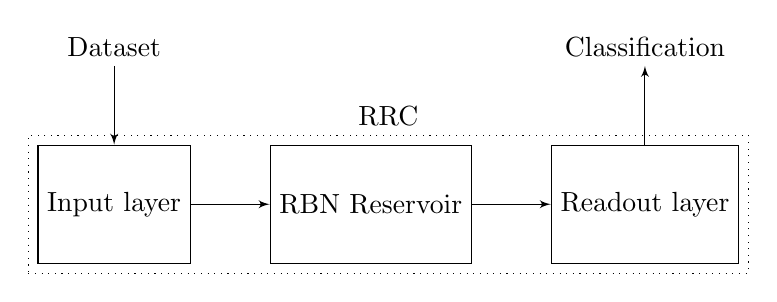
\begin{tikzpicture}
    \node (dataset) {Dataset};
    \node[box, below=of dataset] (input) {Input layer};
    \node[box, right=of input] (reservoir) {RBN Reservoir};
    \node[box, right=of reservoir] (readout) {Readout layer};
    \node[above=of readout] (classification) {Classification};

    \node[draw,dotted,fit=(input) (reservoir) (readout), label={RRC}] {};

    \draw[edge] (dataset) to (input);
    \draw[edge] (input) to (reservoir);
    \draw[edge] (reservoir) to (readout);
    \draw[edge] (readout) to (classification);
  \end{tikzpicture}
  \caption{Block diagram of the RRC processing a dataset.}
  \label{figure:rrc-block}
\end{figure}

\subsection{testing}

To verify that RBN simulation is working,
a RBN is created randomly, initial state set to all zeros, and ran.
The results are visualized in Figure \ref{figure:rbn-noperturb}.
We see that the RBN exhibits stable dynamics, and enters into an attractor around $t=15$.
In Figure \ref{figure:rbn-perturb} we continiously perturb the RBN with the input stream from the Temporal Parity task visualized in Figure \ref{figure:temporal-parity}.
In the perturbed case, the state trajectory is continiously changed, preventing the RBN from settling into an attractor.
Interestingly enough, there seems to be a visual similarity between the two cases.
Such a pattern is sure to dissapear with a RBN in the chaotic phase.

This erratic pattern of state transitions is then fed into the readout layer,
which is then tasked with finding a linear combination of the RBN states that results in the expected output for the given task.

\begin{figure}
  \subfloat[Unperturbed]{
    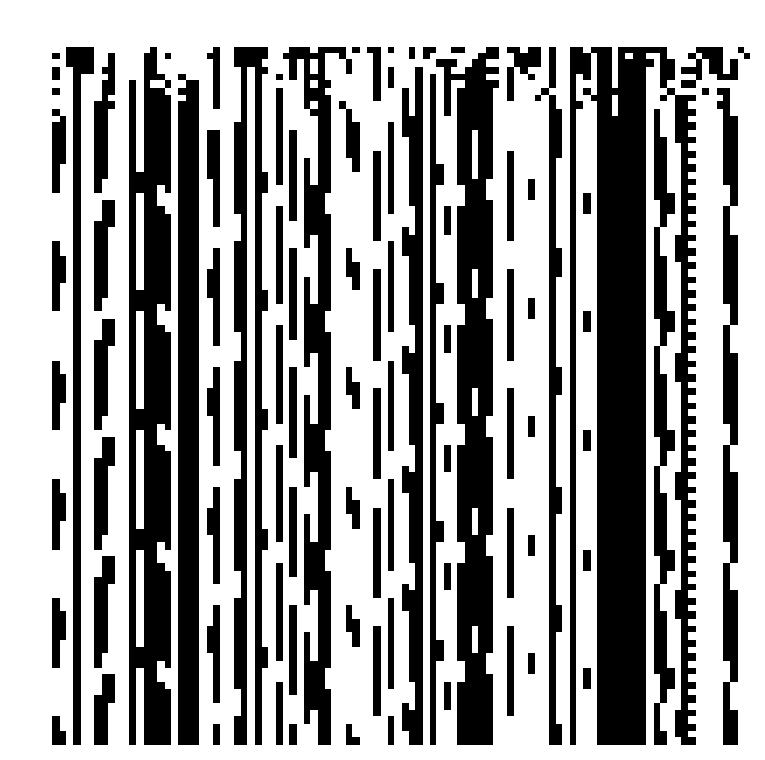
\includegraphics[width=0.5\columnwidth]{method/final-1-noperturb.pdf}
    \label{figure:rbn-noperturb}
  }
  \subfloat[Perturbed]{
    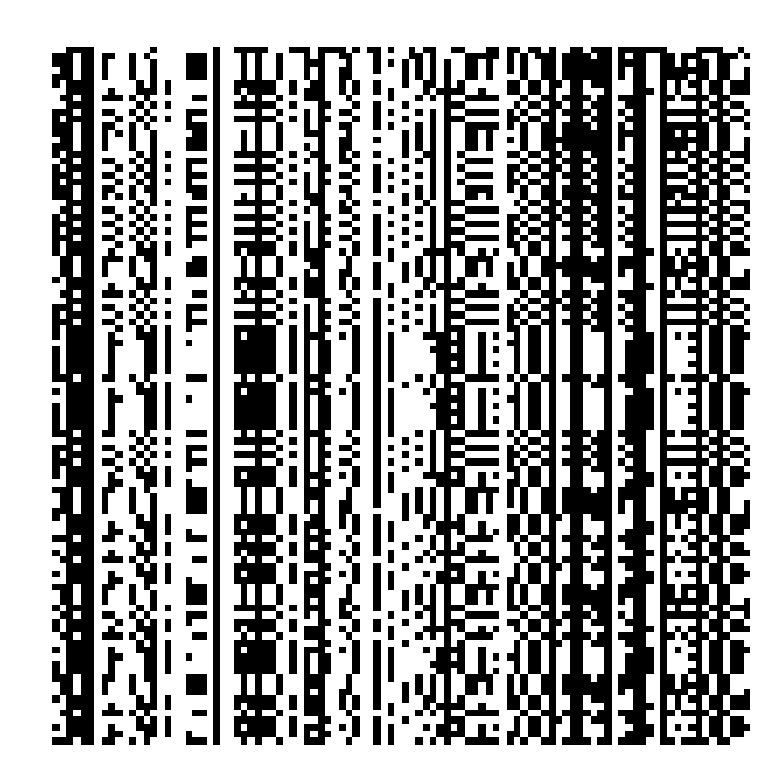
\includegraphics[width=0.5\columnwidth]{method/final-1-perturb.pdf}
    \label{figure:rbn-perturb}
  }
  \caption{
    The same RBN ($N=100, K=2, P=0.5, L=50$) shown both perturbed and unperturbed.
    The boolean states of the RBN are plotted along the X-axis,
    with time flowing downwards.
  }
\end{figure}

\subsection{Training}

To train the RRC system we require a number of training datasets,
as well as different testing datasets to test the trained system.
We will use the datasets described in section \ref{subsection:rbn-reservoir-systems}.

We then either create a new RBN (initialize it randomly),
or load a previously created RBN from disk.
For each bit of input in each dataset,
we perturb the input-connected nodes in the RBN.
After each perturbance, the RBN is ran synchronously (CRBN mode) for one timestep.
The resulting RBN states are collected,
and after the entire dataset is processed,
forwarded to the readout layer.

To find a suitable mapping from the set of reservoir states and the correct input classification,
ridge regression \cite{hoerl1970ridge} is used.
This version of least squares regression is more accurate when faced with input colinearities, as well as always being at least as accurate as ordinary least squares.  
This process is repeated for all the datasets,
and the final regression parameters are chosen as a combination of the parameters obtained for each individual dataset.
Finally we measure the normalized accuracy of the trained reservoir on the test dataset,
defined as the following:
\begin{equation}
Accuracy = 1 - \dfrac{sum(actual\_output \neq expected\_output)}{len(correct\_output)}
\label{formula:accuracy}
\end{equation}

\section{Minimum required reservoir size}

As shown in \cite{MyPreviousPaper},
there are a plethora of RRC systems with $N=100, K=\{2, 3\}$ that solve the temporal parity task for a window size of both 3 and 5.
The reservoirs with $K=3$ had a higher density of success.

Presumably the same tasks can be solved with smaller reservoirs,
the question being how small they can be while retaining accurarcy.


\begin{table}[ht]
    \centering
    \caption{Reservoir parameters for optimal input connectivity}
    \begin{tabular}{ll}
        Nodes               & [10..50], step size=5         \\
        Connectivity        & 3                             \\
        Input connectivity  & [0..n\_nodes], step size = 10 \\
		Output connectivity & n\_nodes                      \\
        Sample size         & 50
    \end{tabular}
\end{table}


As the optimal reservoir size and input connectivity might depend on the task at hand,
we test our reservoirs on both the Temporal Parity and Temporal Density tasks with window sizes of both 3 and 5 (as specified in table \ref{tab:tasks}).

\begin{table}[ht]
  \centering
  \caption{Task parameters}
  \label{tab:tasks}
  \begin{tabular}{ll}
    Task type               & Temporal Parity and Density \\
    Training dataset length & 4 000                       \\
    Test dataset length     & 200                         \\
    $N$ (window size)       & 3 and 5                     \\
    $t$ (offset)            & 0
  \end{tabular} 
\end{table} 

\section{Optimal output connectivyt}

\begin{table}[ht]
    \centering
    \caption{Reservoir parameters for optimal output connectivity}
    \begin{tabular}{ll}
        Nodes               & [10..100], step size=10           \\
        Connectivity        & 3                                 \\
        Input connectivity  & $ n\_nodes / 2 $                  \\
        Output connectivity & [0..n\_nodes], step size=10       \\
        Sample size         & 50
    \end{tabular}
\end{table}


\chapter{Experiments}


\chapter{Conclusion}
\label{chapter:conclusion}

\section{Conclusion}

Experiments confirm that the required reservoir size increases with the difficulty of the task at hand,
with the largest factor being how many bits of input the reservoir is required to remember.
Simulation of RRC systems can therefore aid in deciding the optimal size of physical reservoirs,
given a bridge between the computational power of the reservoir and RBNs can be deduced.

Optimal reservoir perturbation is found to lie at roughly 50\% of the size of the reservoir for RBNs with $K=3$.
When using smaller slices of a reservoir for computation,
lower amounts of total perturbation will be required as long as these perturbations are located within the same topological area.

Results also show that subsets of larger reservoirs will perform at least as well as a separate reservoir of equal size.
Any interference from the unused parts of the reservoir is either minimal or slightly positive.

Finally, no relationship is found between the attractors of an RBN and its performance in a RRC system.
It can therefore not be used for guiding the construction of accurate RBNs.

\section{Further work}

When using a computational substrate such as living rat neurons \cite{demarse2005adaptive},
the connections and size of the substrate may change over time.
It would be interesting to study how much of an RBN in a RC system can be manipulated before its predictive power collapses,
and the readout layer has to be retrained.
These changes would include flipping bits in transition tables and changing internal edges in the network.
If one can relate the network's robustness to perturbations to a regression model's resistance to variance in the predictor variables,
a metric of RRC robustness can be developed.
It would relate the amount of change in the RBN to the expected reduction of reservoir accuracy.

Another question is in what degree does a reservoirs optimal input connectivity change with regards to what physical subset of the substrate is used?
The topology of an RBN is randomly generated and doesn't inherently have a physical mapping,
so one would have to be created for this experiment.
In the water bucket RC system \cite{fernando2003pattern},
one would expect that perturbing one part of the reservoir would result in a larger effect in that area rather than the other side of the bucket.
If one were to observe this smaller part of the total reservoir only,
the hypothesis would be that the perturbation within this restricted area would have to be smaller than if one were to use the entire reservoir for computation.


%% PART 4
\pagestyle{fancy}
\fancyhf{}
\renewcommand{\chaptermark}[1]{\markboth{\chaptername\ \thechapter.\ #1}{}}
\renewcommand{\sectionmark}[1]{\markright{\thesection\ #1}}
\renewcommand{\headrulewidth}{0.1ex}
\renewcommand{\footrulewidth}{0.1ex}
\fancyfoot[LE,RO]{\thepage}
\fancypagestyle{plain}{\fancyhf{}\fancyfoot[LE,RO]{\thepage}\renewcommand{\headrulewidth}{0ex}}

\addcontentsline{toc}{chapter}{Bibliography}

\printbibliography

\cleardoublepage

\section*{\begin{center}{\Huge Appendix}\end{center}}
\addcontentsline{toc}{chapter}{Appendix}
$\\[0.5cm]$

\subsection{Minimum required reservoir size, optimal input connectivity}
\label{app:reservoir_size-input_connectivity}

% Accuracy on TP3

\begin{figure*}[ht]
    \centering
    \caption{Plots of input connectivity against accuracy on TP3 - Part 1 of 2}
    \label{fig:TP3-IC-1}
    \resizebox{\textwidth}{!}{
        \subfloat[N=10]{
            \myboxplot{

\addplot[mark=*, boxplot, boxplot/draw position=0]
table[row sep=\\, y index=0] {
data
0.515 \\
0.465 \\
0.51 \\
0.51 \\
0.55 \\
0.51 \\
0.485 \\
0.485 \\
0.465 \\
0.485 \\
0.47 \\
0.5 \\
0.55 \\
0.49 \\
0.435 \\
0.485 \\
0.51 \\
0.55 \\
0.515 \\
0.535 \\
0.51 \\
0.51 \\
0.485 \\
0.465 \\
0.485 \\
0.575 \\
0.485 \\
0.485 \\
0.465 \\
0.515 \\
0.535 \\
0.465 \\
0.485 \\
0.51 \\
0.485 \\
0.485 \\
0.485 \\
0.49 \\
0.485 \\
0.565 \\
0.465 \\
0.515 \\
0.485 \\
0.485 \\
0.485 \\
0.51 \\
0.485 \\
0.55 \\
0.485 \\
0.485 \\
};

\addplot[mark=*, boxplot, boxplot/draw position=1]
table[row sep=\\, y index=0] {
data
0.785 \\
0.89 \\
0.48 \\
0.495 \\
0.62 \\
0.635 \\
0.735 \\
0.82 \\
0.495 \\
0.65 \\
0.635 \\
0.635 \\
0.73 \\
0.785 \\
0.735 \\
0.815 \\
0.65 \\
0.825 \\
0.69 \\
0.65 \\
0.515 \\
0.665 \\
0.67 \\
0.495 \\
0.495 \\
0.525 \\
0.645 \\
0.72 \\
0.755 \\
0.71 \\
0.635 \\
0.65 \\
0.535 \\
0.78 \\
0.73 \\
0.755 \\
0.775 \\
0.67 \\
0.715 \\
0.495 \\
0.485 \\
0.705 \\
0.66 \\
0.615 \\
0.495 \\
0.495 \\
0.495 \\
0.495 \\
0.87 \\
0.675 \\
};

\addplot[mark=*, boxplot, boxplot/draw position=2]
table[row sep=\\, y index=0] {
data
0.495 \\
0.495 \\
0.495 \\
0.495 \\
0.495 \\
0.495 \\
0.495 \\
0.495 \\
0.495 \\
0.495 \\
0.495 \\
0.495 \\
0.495 \\
0.495 \\
0.495 \\
0.495 \\
0.495 \\
0.495 \\
0.495 \\
0.495 \\
0.495 \\
0.495 \\
0.495 \\
0.495 \\
0.495 \\
0.495 \\
0.495 \\
0.495 \\
0.495 \\
0.495 \\
0.495 \\
0.495 \\
0.495 \\
0.495 \\
0.495 \\
0.495 \\
0.495 \\
0.495 \\
0.495 \\
0.495 \\
0.495 \\
0.495 \\
0.495 \\
0.495 \\
0.495 \\
0.495 \\
0.495 \\
0.495 \\
0.495 \\
0.495 \\
};
}{0.2}{Input connectivity}{21}

        }
        \subfloat[N=20]{
            \myboxplot{

\addplot[mark=*, boxplot, boxplot/draw position=0]
table[row sep=\\, y index=0] {
data
0.485 \\
0.465 \\
0.46 \\
0.485 \\
0.465 \\
0.465 \\
0.485 \\
0.485 \\
0.53 \\
0.485 \\
0.515 \\
0.51 \\
0.51 \\
0.51 \\
0.465 \\
0.515 \\
0.52 \\
0.53 \\
0.53 \\
0.575 \\
0.465 \\
0.465 \\
0.485 \\
0.515 \\
0.485 \\
0.55 \\
0.465 \\
0.51 \\
0.485 \\
0.51 \\
0.515 \\
0.51 \\
0.49 \\
0.54 \\
0.435 \\
0.465 \\
0.485 \\
0.465 \\
0.495 \\
0.485 \\
0.51 \\
0.485 \\
0.465 \\
0.545 \\
0.485 \\
0.485 \\
0.465 \\
0.485 \\
0.55 \\
0.595 \\
};

\addplot[mark=*, boxplot, boxplot/draw position=1]
table[row sep=\\, y index=0] {
data
0.67 \\
0.465 \\
0.52 \\
0.93 \\
0.895 \\
0.68 \\
0.865 \\
0.59 \\
0.675 \\
0.79 \\
0.63 \\
0.595 \\
0.565 \\
0.815 \\
0.745 \\
0.735 \\
0.585 \\
0.485 \\
0.8 \\
0.65 \\
0.69 \\
0.83 \\
0.82 \\
0.555 \\
0.64 \\
0.645 \\
0.46 \\
0.695 \\
0.625 \\
0.785 \\
0.745 \\
0.46 \\
0.62 \\
0.545 \\
0.835 \\
0.57 \\
0.785 \\
0.565 \\
0.555 \\
0.435 \\
0.69 \\
0.645 \\
0.58 \\
0.555 \\
0.585 \\
0.53 \\
0.67 \\
0.525 \\
0.705 \\
0.685 \\
};

\addplot[mark=*, boxplot, boxplot/draw position=2]
table[row sep=\\, y index=0] {
data
0.92 \\
0.995 \\
0.9 \\
0.76 \\
0.945 \\
0.575 \\
0.96 \\
0.925 \\
0.96 \\
0.995 \\
0.61 \\
0.625 \\
0.615 \\
0.78 \\
0.995 \\
0.885 \\
0.785 \\
0.955 \\
0.995 \\
0.735 \\
0.87 \\
0.94 \\
0.81 \\
0.63 \\
0.995 \\
0.465 \\
0.525 \\
0.525 \\
0.97 \\
0.72 \\
0.55 \\
0.94 \\
0.965 \\
0.885 \\
0.665 \\
0.935 \\
0.7 \\
0.94 \\
0.8 \\
0.66 \\
0.815 \\
0.81 \\
0.87 \\
0.77 \\
0.895 \\
0.945 \\
0.845 \\
0.955 \\
0.925 \\
0.765 \\
};

\addplot[mark=*, boxplot, boxplot/draw position=3]
table[row sep=\\, y index=0] {
data
0.495 \\
0.825 \\
0.495 \\
0.995 \\
0.76 \\
0.495 \\
0.995 \\
0.48 \\
0.495 \\
0.695 \\
0.475 \\
0.495 \\
0.505 \\
0.495 \\
0.495 \\
0.62 \\
0.995 \\
0.525 \\
0.84 \\
0.735 \\
0.495 \\
0.73 \\
0.37 \\
0.65 \\
0.495 \\
0.76 \\
0.675 \\
0.73 \\
0.995 \\
0.995 \\
0.495 \\
0.495 \\
0.495 \\
0.655 \\
0.495 \\
0.995 \\
0.655 \\
0.615 \\
0.995 \\
0.88 \\
0.695 \\
0.995 \\
0.495 \\
0.76 \\
0.87 \\
0.675 \\
0.495 \\
0.87 \\
0.58 \\
0.995 \\
};

\addplot[mark=*, boxplot, boxplot/draw position=4]
table[row sep=\\, y index=0] {
data
0.495 \\
0.495 \\
0.495 \\
0.495 \\
0.495 \\
0.495 \\
0.495 \\
0.495 \\
0.495 \\
0.495 \\
0.495 \\
0.495 \\
0.495 \\
0.495 \\
0.495 \\
0.495 \\
0.495 \\
0.495 \\
0.495 \\
0.495 \\
0.495 \\
0.495 \\
0.495 \\
0.495 \\
0.495 \\
0.495 \\
0.495 \\
0.495 \\
0.495 \\
0.495 \\
0.495 \\
0.495 \\
0.495 \\
0.495 \\
0.495 \\
0.495 \\
0.495 \\
0.495 \\
0.495 \\
0.495 \\
0.495 \\
0.495 \\
0.495 \\
0.495 \\
0.495 \\
0.495 \\
0.495 \\
0.495 \\
0.495 \\
0.495 \\
};
}{0.2}{Input connectivity}{21}

        }
    }
    \resizebox{\textwidth}{!}{
        \subfloat[N=30]{
            \myboxplot{

\addplot[mark=*, boxplot, boxplot/draw position=0]
table[row sep=\\, y index=0] {
data
0.51 \\
0.515 \\
0.485 \\
0.49 \\
0.515 \\
0.55 \\
0.485 \\
0.485 \\
0.495 \\
0.465 \\
0.56 \\
0.485 \\
0.465 \\
0.515 \\
0.485 \\
0.5 \\
0.475 \\
0.505 \\
0.515 \\
0.525 \\
0.51 \\
0.495 \\
0.49 \\
0.465 \\
0.505 \\
0.485 \\
0.55 \\
0.515 \\
0.435 \\
0.485 \\
0.575 \\
0.51 \\
0.485 \\
0.585 \\
0.485 \\
0.455 \\
0.485 \\
0.55 \\
0.55 \\
0.535 \\
0.515 \\
0.485 \\
0.495 \\
0.545 \\
0.495 \\
0.545 \\
0.43 \\
0.51 \\
0.495 \\
0.485 \\
};

\addplot[mark=*, boxplot, boxplot/draw position=1]
table[row sep=\\, y index=0] {
data
0.895 \\
0.695 \\
0.535 \\
0.81 \\
0.64 \\
0.67 \\
0.475 \\
0.535 \\
0.73 \\
0.575 \\
0.705 \\
0.61 \\
0.52 \\
0.665 \\
0.73 \\
0.495 \\
0.625 \\
0.59 \\
0.475 \\
0.755 \\
0.515 \\
0.6 \\
0.69 \\
0.665 \\
0.7 \\
0.78 \\
0.565 \\
0.66 \\
0.49 \\
0.65 \\
0.63 \\
0.6 \\
0.575 \\
0.72 \\
0.53 \\
0.535 \\
0.445 \\
0.585 \\
0.73 \\
0.495 \\
0.565 \\
0.615 \\
0.535 \\
0.655 \\
0.59 \\
0.57 \\
0.765 \\
0.69 \\
0.63 \\
0.52 \\
};

\addplot[mark=*, boxplot, boxplot/draw position=2]
table[row sep=\\, y index=0] {
data
0.73 \\
0.49 \\
0.75 \\
0.78 \\
0.995 \\
0.59 \\
0.91 \\
0.65 \\
0.655 \\
0.76 \\
0.81 \\
0.64 \\
0.83 \\
0.86 \\
0.505 \\
0.585 \\
0.975 \\
0.69 \\
0.755 \\
0.715 \\
0.83 \\
0.585 \\
0.855 \\
0.725 \\
0.825 \\
0.71 \\
0.73 \\
0.995 \\
0.73 \\
0.865 \\
0.76 \\
0.92 \\
0.665 \\
0.69 \\
0.61 \\
0.7 \\
0.765 \\
0.875 \\
0.79 \\
0.875 \\
0.855 \\
0.775 \\
0.495 \\
0.79 \\
0.865 \\
0.875 \\
0.8 \\
0.905 \\
0.81 \\
0.625 \\
};

\addplot[mark=*, boxplot, boxplot/draw position=3]
table[row sep=\\, y index=0] {
data
0.99 \\
0.755 \\
0.96 \\
0.85 \\
0.825 \\
0.995 \\
0.995 \\
0.62 \\
0.79 \\
0.77 \\
0.97 \\
0.95 \\
0.915 \\
0.965 \\
0.78 \\
0.885 \\
0.97 \\
0.95 \\
0.835 \\
0.62 \\
0.69 \\
0.995 \\
0.69 \\
0.7 \\
0.955 \\
0.92 \\
0.8 \\
0.785 \\
0.495 \\
0.955 \\
0.995 \\
0.965 \\
0.88 \\
0.85 \\
0.88 \\
0.87 \\
0.82 \\
0.995 \\
0.515 \\
0.86 \\
0.905 \\
0.845 \\
0.88 \\
0.995 \\
0.9 \\
0.555 \\
0.88 \\
0.935 \\
0.78 \\
0.995 \\
};

\addplot[mark=*, boxplot, boxplot/draw position=4]
table[row sep=\\, y index=0] {
data
0.96 \\
0.995 \\
0.89 \\
0.905 \\
0.75 \\
0.85 \\
0.995 \\
0.515 \\
0.84 \\
0.495 \\
0.92 \\
0.995 \\
0.93 \\
0.875 \\
0.995 \\
0.995 \\
0.88 \\
0.975 \\
0.785 \\
0.985 \\
0.885 \\
0.995 \\
0.945 \\
0.93 \\
0.995 \\
0.995 \\
0.915 \\
0.94 \\
0.715 \\
0.88 \\
0.825 \\
0.95 \\
0.73 \\
0.475 \\
0.85 \\
0.87 \\
0.73 \\
0.995 \\
0.625 \\
0.92 \\
0.845 \\
0.755 \\
0.495 \\
0.495 \\
0.78 \\
0.995 \\
0.495 \\
0.995 \\
0.995 \\
0.76 \\
};

\addplot[mark=*, boxplot, boxplot/draw position=5]
table[row sep=\\, y index=0] {
data
0.87 \\
0.59 \\
0.495 \\
0.73 \\
0.855 \\
0.8 \\
0.665 \\
0.76 \\
0.425 \\
0.71 \\
0.76 \\
0.495 \\
0.73 \\
0.685 \\
0.995 \\
0.495 \\
0.495 \\
0.735 \\
0.495 \\
0.495 \\
0.495 \\
0.495 \\
0.495 \\
0.495 \\
0.735 \\
0.495 \\
0.495 \\
0.495 \\
0.495 \\
0.755 \\
0.495 \\
0.495 \\
0.62 \\
0.495 \\
0.495 \\
0.61 \\
0.495 \\
0.825 \\
0.83 \\
0.495 \\
0.5 \\
0.695 \\
0.61 \\
0.495 \\
0.635 \\
0.665 \\
0.495 \\
0.56 \\
0.495 \\
0.525 \\
};

\addplot[mark=*, boxplot, boxplot/draw position=6]
table[row sep=\\, y index=0] {
data
0.495 \\
0.495 \\
0.495 \\
0.495 \\
0.495 \\
0.495 \\
0.495 \\
0.495 \\
0.495 \\
0.495 \\
0.495 \\
0.495 \\
0.495 \\
0.495 \\
0.495 \\
0.495 \\
0.495 \\
0.495 \\
0.495 \\
0.495 \\
0.495 \\
0.495 \\
0.495 \\
0.495 \\
0.495 \\
0.495 \\
0.495 \\
0.495 \\
0.495 \\
0.495 \\
0.495 \\
0.495 \\
0.495 \\
0.495 \\
0.495 \\
0.495 \\
0.495 \\
0.495 \\
0.495 \\
0.495 \\
0.495 \\
0.495 \\
0.495 \\
0.495 \\
0.495 \\
0.495 \\
0.495 \\
0.495 \\
0.495 \\
0.495 \\
};
}{0.2}{Input connectivity}{21}

        }
        \subfloat[N=40]{
            \myboxplot{

\addplot[mark=*, boxplot, boxplot/draw position=0]
table[row sep=\\, y index=0] {
data
0.49 \\
0.465 \\
0.44 \\
0.435 \\
0.535 \\
0.5 \\
0.465 \\
0.49 \\
0.465 \\
0.52 \\
0.495 \\
0.485 \\
0.49 \\
0.55 \\
0.565 \\
0.485 \\
0.515 \\
0.575 \\
0.495 \\
0.5 \\
0.495 \\
0.485 \\
0.485 \\
0.49 \\
0.465 \\
0.455 \\
0.545 \\
0.51 \\
0.525 \\
0.47 \\
0.465 \\
0.46 \\
0.495 \\
0.495 \\
0.455 \\
0.47 \\
0.52 \\
0.51 \\
0.495 \\
0.48 \\
0.495 \\
0.485 \\
0.505 \\
0.485 \\
0.505 \\
0.485 \\
0.495 \\
0.51 \\
0.51 \\
0.55 \\
};

\addplot[mark=*, boxplot, boxplot/draw position=1]
table[row sep=\\, y index=0] {
data
0.51 \\
0.595 \\
0.455 \\
0.8 \\
0.47 \\
0.55 \\
0.54 \\
0.93 \\
0.495 \\
0.755 \\
0.555 \\
0.745 \\
0.535 \\
0.61 \\
0.535 \\
0.685 \\
0.66 \\
0.5 \\
0.775 \\
0.605 \\
0.565 \\
0.55 \\
0.585 \\
0.51 \\
0.835 \\
0.475 \\
0.62 \\
0.505 \\
0.61 \\
0.715 \\
0.905 \\
0.54 \\
0.535 \\
0.605 \\
0.465 \\
0.695 \\
0.615 \\
0.545 \\
0.565 \\
0.5 \\
0.82 \\
0.585 \\
0.915 \\
0.57 \\
0.625 \\
0.575 \\
0.495 \\
0.66 \\
0.715 \\
0.53 \\
};

\addplot[mark=*, boxplot, boxplot/draw position=2]
table[row sep=\\, y index=0] {
data
0.725 \\
0.825 \\
0.6 \\
0.645 \\
0.9 \\
0.775 \\
0.84 \\
0.715 \\
0.885 \\
0.87 \\
0.585 \\
0.54 \\
0.815 \\
0.73 \\
0.75 \\
0.695 \\
0.67 \\
0.825 \\
0.725 \\
0.795 \\
0.82 \\
0.595 \\
0.64 \\
0.77 \\
0.665 \\
0.57 \\
0.865 \\
0.435 \\
0.675 \\
0.65 \\
0.775 \\
0.535 \\
0.59 \\
0.89 \\
0.855 \\
0.59 \\
0.665 \\
0.855 \\
0.995 \\
0.51 \\
0.84 \\
0.78 \\
0.475 \\
0.8 \\
0.85 \\
0.93 \\
0.525 \\
0.795 \\
0.785 \\
0.875 \\
};

\addplot[mark=*, boxplot, boxplot/draw position=3]
table[row sep=\\, y index=0] {
data
0.86 \\
0.92 \\
0.95 \\
0.885 \\
0.995 \\
0.92 \\
0.885 \\
0.76 \\
0.895 \\
0.945 \\
0.995 \\
0.855 \\
0.985 \\
0.77 \\
0.965 \\
0.715 \\
0.865 \\
0.85 \\
0.835 \\
0.825 \\
0.945 \\
0.995 \\
0.96 \\
0.74 \\
0.955 \\
0.92 \\
0.78 \\
0.995 \\
0.965 \\
0.97 \\
0.86 \\
0.77 \\
0.875 \\
0.94 \\
0.895 \\
0.925 \\
0.855 \\
0.85 \\
0.96 \\
0.965 \\
0.785 \\
0.86 \\
0.99 \\
0.945 \\
0.88 \\
0.85 \\
0.975 \\
0.965 \\
0.755 \\
0.935 \\
};

\addplot[mark=*, boxplot, boxplot/draw position=4]
table[row sep=\\, y index=0] {
data
0.975 \\
0.775 \\
0.995 \\
0.92 \\
0.99 \\
0.835 \\
0.735 \\
0.98 \\
0.945 \\
0.94 \\
0.9 \\
0.79 \\
0.72 \\
0.905 \\
0.53 \\
0.765 \\
0.855 \\
0.955 \\
0.86 \\
0.865 \\
0.985 \\
0.87 \\
0.995 \\
0.725 \\
0.98 \\
0.785 \\
0.9 \\
0.89 \\
0.925 \\
0.995 \\
0.93 \\
0.955 \\
0.985 \\
0.89 \\
0.83 \\
0.845 \\
0.785 \\
0.97 \\
0.995 \\
0.995 \\
0.68 \\
0.995 \\
0.89 \\
0.955 \\
0.995 \\
0.98 \\
0.66 \\
0.945 \\
0.98 \\
0.745 \\
};

\addplot[mark=*, boxplot, boxplot/draw position=5]
table[row sep=\\, y index=0] {
data
0.95 \\
0.995 \\
0.885 \\
0.7 \\
0.845 \\
0.98 \\
0.995 \\
0.74 \\
0.995 \\
0.95 \\
0.95 \\
0.91 \\
0.955 \\
0.93 \\
0.68 \\
0.995 \\
0.79 \\
0.91 \\
0.83 \\
0.495 \\
0.995 \\
0.545 \\
0.925 \\
0.885 \\
0.995 \\
0.845 \\
0.965 \\
0.715 \\
0.995 \\
0.995 \\
0.995 \\
0.925 \\
0.995 \\
0.99 \\
0.715 \\
0.85 \\
0.995 \\
0.905 \\
0.88 \\
0.92 \\
0.995 \\
0.995 \\
0.82 \\
0.61 \\
0.475 \\
0.955 \\
0.73 \\
0.945 \\
0.985 \\
0.995 \\
};

\addplot[mark=*, boxplot, boxplot/draw position=6]
table[row sep=\\, y index=0] {
data
0.995 \\
0.73 \\
0.37 \\
0.435 \\
0.995 \\
0.495 \\
0.615 \\
0.995 \\
0.495 \\
0.76 \\
0.995 \\
0.995 \\
0.97 \\
0.88 \\
0.855 \\
0.995 \\
0.995 \\
0.87 \\
0.73 \\
0.88 \\
0.495 \\
0.665 \\
0.88 \\
0.525 \\
0.82 \\
0.67 \\
0.81 \\
0.62 \\
0.795 \\
0.76 \\
0.495 \\
0.76 \\
0.855 \\
0.875 \\
0.995 \\
0.715 \\
0.615 \\
0.615 \\
0.71 \\
0.76 \\
0.88 \\
0.495 \\
0.995 \\
0.995 \\
0.57 \\
0.76 \\
0.88 \\
0.585 \\
0.73 \\
0.495 \\
};

\addplot[mark=*, boxplot, boxplot/draw position=7]
table[row sep=\\, y index=0] {
data
0.495 \\
0.495 \\
0.76 \\
0.495 \\
0.495 \\
0.495 \\
0.495 \\
0.495 \\
0.495 \\
0.76 \\
0.495 \\
0.495 \\
0.73 \\
0.495 \\
0.495 \\
0.87 \\
0.665 \\
0.76 \\
0.615 \\
0.87 \\
0.73 \\
0.495 \\
0.495 \\
0.495 \\
0.495 \\
0.495 \\
0.495 \\
0.73 \\
0.495 \\
0.495 \\
0.495 \\
0.73 \\
0.995 \\
0.495 \\
0.67 \\
0.73 \\
0.495 \\
0.495 \\
0.495 \\
0.495 \\
0.37 \\
0.995 \\
0.495 \\
0.67 \\
0.495 \\
0.935 \\
0.495 \\
0.495 \\
0.495 \\
0.825 \\
};

\addplot[mark=*, boxplot, boxplot/draw position=8]
table[row sep=\\, y index=0] {
data
0.495 \\
0.495 \\
0.495 \\
0.495 \\
0.495 \\
0.495 \\
0.495 \\
0.495 \\
0.495 \\
0.495 \\
0.495 \\
0.495 \\
0.495 \\
0.495 \\
0.495 \\
0.495 \\
0.495 \\
0.495 \\
0.495 \\
0.495 \\
0.495 \\
0.495 \\
0.495 \\
0.495 \\
0.495 \\
0.495 \\
0.495 \\
0.495 \\
0.495 \\
0.495 \\
0.495 \\
0.495 \\
0.495 \\
0.495 \\
0.495 \\
0.495 \\
0.495 \\
0.495 \\
0.495 \\
0.495 \\
0.495 \\
0.495 \\
0.495 \\
0.495 \\
0.495 \\
0.495 \\
0.495 \\
0.495 \\
0.495 \\
0.495 \\
};
}{0.2}{Input connectivity}{21}

        }
    }
    \resizebox{\textwidth}{!}{
        \subfloat[N=50]{
            \myboxplot{

\addplot[mark=*, boxplot, boxplot/draw position=0]
table[row sep=\\, y index=0] {
data
0.565 \\
0.45 \\
0.53 \\
0.485 \\
0.555 \\
0.555 \\
0.445 \\
0.515 \\
0.505 \\
0.49 \\
0.455 \\
0.48 \\
0.48 \\
0.58 \\
0.52 \\
0.515 \\
0.515 \\
0.47 \\
0.5 \\
0.51 \\
0.56 \\
0.485 \\
0.5 \\
0.585 \\
0.515 \\
0.52 \\
0.505 \\
0.535 \\
0.535 \\
0.485 \\
0.485 \\
0.48 \\
0.56 \\
0.49 \\
0.465 \\
0.48 \\
0.52 \\
0.51 \\
0.485 \\
0.475 \\
0.51 \\
0.535 \\
0.545 \\
0.485 \\
0.535 \\
0.435 \\
0.545 \\
0.465 \\
0.57 \\
0.47 \\
};

\addplot[mark=*, boxplot, boxplot/draw position=1]
table[row sep=\\, y index=0] {
data
0.475 \\
0.465 \\
0.485 \\
0.625 \\
0.66 \\
0.58 \\
0.48 \\
0.665 \\
0.68 \\
0.465 \\
0.72 \\
0.53 \\
0.51 \\
0.565 \\
0.805 \\
0.76 \\
0.62 \\
0.415 \\
0.505 \\
0.555 \\
0.695 \\
0.63 \\
0.505 \\
0.49 \\
0.62 \\
0.73 \\
0.605 \\
0.635 \\
0.835 \\
0.525 \\
0.475 \\
0.65 \\
0.58 \\
0.49 \\
0.535 \\
0.54 \\
0.67 \\
0.49 \\
0.805 \\
0.61 \\
0.545 \\
0.655 \\
0.465 \\
0.765 \\
0.575 \\
0.705 \\
0.56 \\
0.635 \\
0.59 \\
0.555 \\
};

\addplot[mark=*, boxplot, boxplot/draw position=2]
table[row sep=\\, y index=0] {
data
0.77 \\
0.685 \\
0.77 \\
0.815 \\
0.9 \\
0.535 \\
0.67 \\
0.83 \\
0.63 \\
0.59 \\
0.62 \\
0.705 \\
0.605 \\
0.475 \\
0.775 \\
0.835 \\
0.805 \\
0.495 \\
0.98 \\
0.76 \\
0.975 \\
0.685 \\
0.515 \\
0.645 \\
0.705 \\
0.675 \\
0.8 \\
0.685 \\
0.615 \\
0.475 \\
0.735 \\
0.58 \\
0.955 \\
0.82 \\
0.5 \\
0.55 \\
0.795 \\
0.72 \\
0.87 \\
0.73 \\
0.645 \\
0.685 \\
0.96 \\
0.57 \\
0.765 \\
0.675 \\
0.82 \\
0.87 \\
0.87 \\
0.695 \\
};

\addplot[mark=*, boxplot, boxplot/draw position=3]
table[row sep=\\, y index=0] {
data
0.94 \\
0.945 \\
0.99 \\
0.965 \\
0.825 \\
0.88 \\
0.88 \\
0.9 \\
0.925 \\
0.92 \\
0.595 \\
0.635 \\
0.855 \\
0.955 \\
0.86 \\
0.94 \\
0.695 \\
0.885 \\
0.655 \\
0.91 \\
0.91 \\
0.925 \\
0.795 \\
0.94 \\
0.835 \\
0.89 \\
0.825 \\
0.755 \\
0.995 \\
0.965 \\
0.875 \\
0.99 \\
0.91 \\
0.72 \\
0.845 \\
0.835 \\
0.795 \\
0.915 \\
0.845 \\
0.92 \\
0.89 \\
0.995 \\
0.92 \\
0.93 \\
0.81 \\
0.945 \\
0.675 \\
0.945 \\
0.835 \\
0.98 \\
};

\addplot[mark=*, boxplot, boxplot/draw position=4]
table[row sep=\\, y index=0] {
data
0.865 \\
0.965 \\
0.705 \\
0.995 \\
0.99 \\
0.95 \\
0.805 \\
0.9 \\
0.91 \\
0.95 \\
0.96 \\
0.9 \\
0.955 \\
0.985 \\
0.91 \\
0.995 \\
0.865 \\
0.94 \\
0.765 \\
0.7 \\
0.915 \\
0.85 \\
0.995 \\
0.785 \\
0.975 \\
0.705 \\
0.805 \\
0.975 \\
0.975 \\
0.985 \\
0.995 \\
0.91 \\
0.905 \\
0.99 \\
0.91 \\
0.79 \\
0.89 \\
0.97 \\
0.78 \\
0.695 \\
0.865 \\
0.975 \\
0.865 \\
0.84 \\
0.705 \\
0.865 \\
0.915 \\
0.69 \\
0.98 \\
0.84 \\
};

\addplot[mark=*, boxplot, boxplot/draw position=5]
table[row sep=\\, y index=0] {
data
0.935 \\
0.925 \\
0.685 \\
0.995 \\
0.995 \\
0.905 \\
0.86 \\
0.995 \\
0.9 \\
0.99 \\
0.91 \\
0.995 \\
0.995 \\
0.985 \\
0.995 \\
0.86 \\
0.95 \\
0.865 \\
0.995 \\
0.96 \\
0.77 \\
0.825 \\
0.97 \\
0.98 \\
0.915 \\
0.995 \\
0.885 \\
0.995 \\
0.995 \\
0.985 \\
0.96 \\
0.975 \\
0.995 \\
0.995 \\
0.995 \\
0.995 \\
0.995 \\
0.85 \\
0.995 \\
0.96 \\
0.995 \\
0.995 \\
0.76 \\
0.935 \\
0.995 \\
0.935 \\
0.84 \\
0.995 \\
0.985 \\
0.93 \\
};

\addplot[mark=*, boxplot, boxplot/draw position=6]
table[row sep=\\, y index=0] {
data
0.995 \\
0.96 \\
0.995 \\
0.985 \\
0.72 \\
0.96 \\
0.995 \\
0.995 \\
0.985 \\
0.995 \\
0.67 \\
0.94 \\
0.995 \\
0.855 \\
0.995 \\
0.855 \\
0.995 \\
0.86 \\
0.995 \\
0.995 \\
0.99 \\
0.995 \\
0.97 \\
0.995 \\
0.995 \\
0.815 \\
0.995 \\
0.935 \\
0.99 \\
0.86 \\
0.995 \\
0.705 \\
0.995 \\
0.995 \\
0.995 \\
0.98 \\
0.995 \\
0.915 \\
0.95 \\
0.96 \\
0.935 \\
0.86 \\
0.995 \\
0.995 \\
0.99 \\
0.8 \\
0.96 \\
0.995 \\
0.99 \\
0.93 \\
};

\addplot[mark=*, boxplot, boxplot/draw position=7]
table[row sep=\\, y index=0] {
data
0.995 \\
0.87 \\
0.96 \\
0.87 \\
0.935 \\
0.765 \\
0.995 \\
0.77 \\
0.9 \\
0.805 \\
0.935 \\
0.87 \\
0.945 \\
0.995 \\
0.995 \\
0.995 \\
0.89 \\
0.875 \\
0.87 \\
0.995 \\
0.995 \\
0.83 \\
0.995 \\
0.995 \\
0.975 \\
0.88 \\
0.965 \\
0.73 \\
0.995 \\
0.87 \\
0.865 \\
0.965 \\
0.95 \\
0.995 \\
0.525 \\
0.995 \\
0.705 \\
0.995 \\
0.995 \\
0.87 \\
0.995 \\
0.685 \\
0.85 \\
0.995 \\
0.84 \\
0.995 \\
0.995 \\
0.995 \\
0.97 \\
0.95 \\
};

\addplot[mark=*, boxplot, boxplot/draw position=8]
table[row sep=\\, y index=0] {
data
0.995 \\
0.995 \\
0.755 \\
0.76 \\
0.76 \\
0.995 \\
0.995 \\
0.495 \\
0.82 \\
0.76 \\
0.995 \\
0.62 \\
0.76 \\
0.82 \\
0.495 \\
0.73 \\
0.87 \\
0.875 \\
0.62 \\
0.995 \\
0.725 \\
0.995 \\
0.995 \\
0.495 \\
0.665 \\
0.995 \\
0.495 \\
0.73 \\
0.61 \\
0.495 \\
0.73 \\
0.735 \\
0.495 \\
0.7 \\
0.495 \\
0.59 \\
0.495 \\
0.495 \\
0.73 \\
0.655 \\
0.495 \\
0.995 \\
0.73 \\
0.855 \\
0.73 \\
0.665 \\
0.995 \\
0.495 \\
0.67 \\
0.995 \\
};

\addplot[mark=*, boxplot, boxplot/draw position=9]
table[row sep=\\, y index=0] {
data
0.495 \\
0.495 \\
0.495 \\
0.48 \\
0.495 \\
0.495 \\
0.495 \\
0.995 \\
0.73 \\
0.495 \\
0.635 \\
0.495 \\
0.79 \\
0.995 \\
0.495 \\
0.665 \\
0.495 \\
0.66 \\
0.655 \\
0.495 \\
0.495 \\
0.495 \\
0.495 \\
0.665 \\
0.495 \\
0.495 \\
0.495 \\
0.495 \\
0.495 \\
0.495 \\
0.88 \\
0.495 \\
0.76 \\
0.495 \\
0.76 \\
0.495 \\
0.495 \\
0.495 \\
0.495 \\
0.495 \\
0.495 \\
0.495 \\
0.995 \\
0.495 \\
0.495 \\
0.495 \\
0.495 \\
0.755 \\
0.495 \\
0.495 \\
};

\addplot[mark=*, boxplot, boxplot/draw position=10]
table[row sep=\\, y index=0] {
data
0.495 \\
0.495 \\
0.495 \\
0.495 \\
0.495 \\
0.495 \\
0.495 \\
0.495 \\
0.495 \\
0.495 \\
0.495 \\
0.495 \\
0.495 \\
0.495 \\
0.495 \\
0.495 \\
0.495 \\
0.495 \\
0.495 \\
0.495 \\
0.495 \\
0.495 \\
0.495 \\
0.495 \\
0.495 \\
0.495 \\
0.495 \\
0.495 \\
0.495 \\
0.495 \\
0.495 \\
0.495 \\
0.495 \\
0.495 \\
0.495 \\
0.495 \\
0.495 \\
0.495 \\
0.495 \\
0.495 \\
0.495 \\
0.495 \\
0.495 \\
0.495 \\
0.495 \\
0.495 \\
0.495 \\
0.495 \\
0.495 \\
0.495 \\
};
}{0.2}{Input connectivity}{21}

        }
        \subfloat[N=60]{
            \myboxplot{

\addplot[mark=*, boxplot, boxplot/draw position=0]
table[row sep=\\, y index=0] {
data
0.54 \\
0.545 \\
0.525 \\
0.495 \\
0.515 \\
0.48 \\
0.505 \\
0.43 \\
0.515 \\
0.52 \\
0.495 \\
0.46 \\
0.52 \\
0.5 \\
0.485 \\
0.45 \\
0.545 \\
0.49 \\
0.485 \\
0.445 \\
0.515 \\
0.565 \\
0.53 \\
0.535 \\
0.5 \\
0.485 \\
0.595 \\
0.435 \\
0.475 \\
0.465 \\
0.53 \\
0.51 \\
0.525 \\
0.495 \\
0.575 \\
0.56 \\
0.485 \\
0.495 \\
0.565 \\
0.465 \\
0.485 \\
0.48 \\
0.445 \\
0.485 \\
0.47 \\
0.52 \\
0.47 \\
0.495 \\
0.54 \\
0.5 \\
};

\addplot[mark=*, boxplot, boxplot/draw position=1]
table[row sep=\\, y index=0] {
data
0.56 \\
0.56 \\
0.48 \\
0.525 \\
0.48 \\
0.57 \\
0.52 \\
0.525 \\
0.54 \\
0.495 \\
0.6 \\
0.56 \\
0.515 \\
0.535 \\
0.675 \\
0.485 \\
0.525 \\
0.625 \\
0.545 \\
0.54 \\
0.585 \\
0.43 \\
0.51 \\
0.565 \\
0.515 \\
0.58 \\
0.655 \\
0.525 \\
0.485 \\
0.49 \\
0.5 \\
0.45 \\
0.505 \\
0.52 \\
0.575 \\
0.765 \\
0.545 \\
0.505 \\
0.55 \\
0.46 \\
0.635 \\
0.575 \\
0.625 \\
0.585 \\
0.76 \\
0.49 \\
0.58 \\
0.6 \\
0.6 \\
0.585 \\
};

\addplot[mark=*, boxplot, boxplot/draw position=2]
table[row sep=\\, y index=0] {
data
0.805 \\
0.87 \\
0.825 \\
0.835 \\
0.65 \\
0.84 \\
0.69 \\
0.56 \\
0.545 \\
0.65 \\
0.61 \\
0.985 \\
0.635 \\
0.52 \\
0.725 \\
0.62 \\
0.635 \\
0.74 \\
0.605 \\
0.675 \\
0.64 \\
0.715 \\
0.66 \\
0.595 \\
0.83 \\
0.565 \\
0.595 \\
0.815 \\
0.495 \\
0.625 \\
0.79 \\
0.77 \\
0.67 \\
0.65 \\
0.75 \\
0.805 \\
0.78 \\
0.995 \\
0.74 \\
0.695 \\
0.58 \\
0.87 \\
0.77 \\
0.68 \\
0.57 \\
0.54 \\
0.635 \\
0.88 \\
0.555 \\
0.695 \\
};

\addplot[mark=*, boxplot, boxplot/draw position=3]
table[row sep=\\, y index=0] {
data
0.775 \\
0.795 \\
0.7 \\
0.985 \\
0.815 \\
0.87 \\
0.67 \\
0.935 \\
0.785 \\
0.855 \\
0.825 \\
0.72 \\
0.9 \\
0.94 \\
0.65 \\
0.855 \\
0.595 \\
0.645 \\
0.96 \\
0.835 \\
0.76 \\
0.795 \\
0.995 \\
0.645 \\
0.895 \\
0.92 \\
0.79 \\
0.7 \\
0.53 \\
0.74 \\
0.845 \\
0.54 \\
0.7 \\
0.795 \\
0.565 \\
0.935 \\
0.975 \\
0.88 \\
0.58 \\
0.725 \\
0.84 \\
0.835 \\
0.84 \\
0.98 \\
0.915 \\
0.66 \\
0.905 \\
0.64 \\
0.795 \\
0.725 \\
};

\addplot[mark=*, boxplot, boxplot/draw position=4]
table[row sep=\\, y index=0] {
data
0.825 \\
0.905 \\
0.955 \\
0.995 \\
0.86 \\
0.84 \\
0.97 \\
0.92 \\
0.99 \\
0.92 \\
0.995 \\
0.995 \\
0.965 \\
0.96 \\
0.71 \\
0.84 \\
0.83 \\
0.89 \\
0.825 \\
0.5 \\
0.805 \\
0.995 \\
0.995 \\
0.94 \\
0.985 \\
0.745 \\
0.925 \\
0.705 \\
0.99 \\
0.915 \\
0.95 \\
0.87 \\
0.775 \\
0.875 \\
0.905 \\
0.86 \\
0.945 \\
0.76 \\
0.96 \\
0.76 \\
0.98 \\
0.815 \\
0.8 \\
0.995 \\
0.905 \\
0.975 \\
0.85 \\
0.795 \\
0.89 \\
0.825 \\
};

\addplot[mark=*, boxplot, boxplot/draw position=5]
table[row sep=\\, y index=0] {
data
0.985 \\
0.925 \\
0.995 \\
0.815 \\
0.92 \\
0.995 \\
0.995 \\
0.76 \\
0.995 \\
0.995 \\
0.785 \\
0.93 \\
0.87 \\
0.94 \\
0.995 \\
0.975 \\
0.8 \\
0.81 \\
0.995 \\
0.965 \\
0.995 \\
0.96 \\
0.77 \\
0.84 \\
0.92 \\
0.985 \\
0.86 \\
0.995 \\
0.955 \\
0.995 \\
0.895 \\
0.995 \\
0.94 \\
0.995 \\
0.98 \\
0.975 \\
0.75 \\
0.995 \\
0.92 \\
0.95 \\
0.995 \\
0.995 \\
0.97 \\
0.655 \\
0.98 \\
0.995 \\
0.965 \\
0.995 \\
0.98 \\
0.93 \\
};

\addplot[mark=*, boxplot, boxplot/draw position=6]
table[row sep=\\, y index=0] {
data
0.905 \\
0.995 \\
0.985 \\
0.995 \\
0.995 \\
0.995 \\
0.995 \\
0.855 \\
0.995 \\
0.9 \\
0.92 \\
0.995 \\
0.995 \\
0.945 \\
0.995 \\
0.995 \\
0.975 \\
0.985 \\
0.865 \\
0.985 \\
0.995 \\
0.995 \\
0.9 \\
0.925 \\
0.995 \\
0.995 \\
0.995 \\
0.97 \\
0.995 \\
0.915 \\
0.955 \\
0.985 \\
0.995 \\
0.995 \\
0.995 \\
0.995 \\
0.995 \\
0.955 \\
0.99 \\
0.975 \\
0.95 \\
0.995 \\
0.98 \\
0.995 \\
0.975 \\
0.995 \\
0.995 \\
0.995 \\
0.995 \\
0.995 \\
};

\addplot[mark=*, boxplot, boxplot/draw position=7]
table[row sep=\\, y index=0] {
data
0.895 \\
0.995 \\
0.995 \\
0.935 \\
0.995 \\
0.895 \\
0.995 \\
0.88 \\
0.99 \\
0.995 \\
0.925 \\
0.925 \\
0.995 \\
0.84 \\
0.955 \\
0.835 \\
0.715 \\
0.995 \\
0.87 \\
0.945 \\
0.935 \\
0.92 \\
0.995 \\
0.995 \\
0.995 \\
0.89 \\
0.995 \\
0.995 \\
0.985 \\
0.995 \\
0.995 \\
0.995 \\
0.875 \\
0.805 \\
0.995 \\
0.955 \\
0.995 \\
0.96 \\
0.635 \\
0.995 \\
0.995 \\
0.995 \\
0.95 \\
0.995 \\
0.99 \\
0.955 \\
0.84 \\
0.995 \\
0.965 \\
0.995 \\
};

\addplot[mark=*, boxplot, boxplot/draw position=8]
table[row sep=\\, y index=0] {
data
0.935 \\
0.465 \\
0.995 \\
0.995 \\
0.995 \\
0.97 \\
0.995 \\
0.995 \\
0.62 \\
0.995 \\
0.995 \\
0.755 \\
0.995 \\
0.86 \\
0.985 \\
0.835 \\
0.995 \\
0.975 \\
0.995 \\
0.86 \\
0.995 \\
0.92 \\
0.93 \\
0.925 \\
0.92 \\
0.95 \\
0.995 \\
0.995 \\
0.995 \\
0.99 \\
0.99 \\
0.995 \\
0.995 \\
0.995 \\
0.995 \\
0.995 \\
0.94 \\
0.995 \\
0.995 \\
0.995 \\
0.865 \\
0.995 \\
0.995 \\
0.995 \\
0.995 \\
0.995 \\
0.995 \\
0.995 \\
0.995 \\
0.995 \\
};

\addplot[mark=*, boxplot, boxplot/draw position=9]
table[row sep=\\, y index=0] {
data
0.73 \\
0.495 \\
0.995 \\
0.83 \\
0.995 \\
0.995 \\
0.995 \\
0.62 \\
0.995 \\
0.965 \\
0.915 \\
0.79 \\
0.995 \\
0.995 \\
0.755 \\
0.935 \\
0.995 \\
0.81 \\
0.76 \\
0.59 \\
0.495 \\
0.995 \\
0.495 \\
0.995 \\
0.37 \\
0.73 \\
0.995 \\
0.825 \\
0.995 \\
0.985 \\
0.995 \\
0.995 \\
0.665 \\
0.495 \\
0.7 \\
0.875 \\
0.56 \\
0.995 \\
0.995 \\
0.915 \\
0.995 \\
0.855 \\
0.995 \\
0.995 \\
0.995 \\
0.995 \\
0.93 \\
0.995 \\
0.82 \\
0.76 \\
};

\addplot[mark=*, boxplot, boxplot/draw position=10]
table[row sep=\\, y index=0] {
data
0.995 \\
0.87 \\
0.73 \\
0.855 \\
0.855 \\
0.76 \\
0.76 \\
0.82 \\
0.495 \\
0.995 \\
0.495 \\
0.88 \\
0.495 \\
0.995 \\
0.82 \\
0.995 \\
0.495 \\
0.995 \\
0.995 \\
0.495 \\
0.76 \\
0.67 \\
0.955 \\
0.875 \\
0.935 \\
0.995 \\
0.76 \\
0.495 \\
0.62 \\
0.495 \\
0.995 \\
0.495 \\
0.995 \\
0.495 \\
0.495 \\
0.495 \\
0.67 \\
0.995 \\
0.505 \\
0.655 \\
0.83 \\
0.56 \\
0.495 \\
0.995 \\
0.995 \\
0.87 \\
0.495 \\
0.93 \\
0.495 \\
0.79 \\
};

\addplot[mark=*, boxplot, boxplot/draw position=11]
table[row sep=\\, y index=0] {
data
0.495 \\
0.73 \\
0.67 \\
0.495 \\
0.495 \\
0.495 \\
0.495 \\
0.495 \\
0.495 \\
0.495 \\
0.495 \\
0.48 \\
0.495 \\
0.495 \\
0.495 \\
0.495 \\
0.495 \\
0.495 \\
0.73 \\
0.495 \\
0.7 \\
0.495 \\
0.495 \\
0.495 \\
0.76 \\
0.76 \\
0.495 \\
0.635 \\
0.67 \\
0.37 \\
0.76 \\
0.495 \\
0.495 \\
0.495 \\
0.495 \\
0.495 \\
0.495 \\
0.495 \\
0.495 \\
0.67 \\
0.495 \\
0.615 \\
0.495 \\
0.665 \\
0.495 \\
0.76 \\
0.495 \\
0.495 \\
0.495 \\
0.65 \\
};

\addplot[mark=*, boxplot, boxplot/draw position=12]
table[row sep=\\, y index=0] {
data
0.495 \\
0.495 \\
0.495 \\
0.495 \\
0.495 \\
0.495 \\
0.495 \\
0.495 \\
0.495 \\
0.495 \\
0.495 \\
0.495 \\
0.495 \\
0.495 \\
0.495 \\
0.495 \\
0.495 \\
0.495 \\
0.495 \\
0.495 \\
0.495 \\
0.495 \\
0.495 \\
0.495 \\
0.495 \\
0.495 \\
0.495 \\
0.495 \\
0.495 \\
0.495 \\
0.495 \\
0.495 \\
0.495 \\
0.495 \\
0.495 \\
0.495 \\
0.495 \\
0.495 \\
0.495 \\
0.495 \\
0.495 \\
0.495 \\
0.495 \\
0.495 \\
0.495 \\
0.495 \\
0.495 \\
0.495 \\
0.495 \\
0.495 \\
};
}{0.2}{Input connectivity}{21}

        }
    }
\end{figure*}

\begin{figure*}[ht]
    \centering
    \caption{Plots of input connectivity against accuracy on TP3 - Part 2 of 2}
    \label{fig:TP3-IC-2}
    \resizebox{\textwidth}{!}{
        \subfloat[N=70]{
            \myboxplot{

\addplot[mark=*, boxplot, boxplot/draw position=0]
table[row sep=\\, y index=0] {
data
0.535 \\
0.465 \\
0.465 \\
0.49 \\
0.565 \\
0.53 \\
0.42 \\
0.51 \\
0.48 \\
0.51 \\
0.485 \\
0.45 \\
0.47 \\
0.54 \\
0.51 \\
0.52 \\
0.53 \\
0.545 \\
0.565 \\
0.53 \\
0.535 \\
0.485 \\
0.54 \\
0.445 \\
0.515 \\
0.51 \\
0.495 \\
0.505 \\
0.515 \\
0.505 \\
0.545 \\
0.545 \\
0.455 \\
0.55 \\
0.49 \\
0.56 \\
0.485 \\
0.495 \\
0.525 \\
0.48 \\
0.525 \\
0.435 \\
0.435 \\
0.575 \\
0.445 \\
0.495 \\
0.495 \\
0.485 \\
0.56 \\
0.465 \\
};

\addplot[mark=*, boxplot, boxplot/draw position=1]
table[row sep=\\, y index=0] {
data
0.515 \\
0.6 \\
0.545 \\
0.52 \\
0.55 \\
0.555 \\
0.505 \\
0.51 \\
0.665 \\
0.55 \\
0.56 \\
0.52 \\
0.5 \\
0.45 \\
0.495 \\
0.625 \\
0.455 \\
0.44 \\
0.535 \\
0.47 \\
0.475 \\
0.525 \\
0.52 \\
0.505 \\
0.485 \\
0.49 \\
0.53 \\
0.48 \\
0.47 \\
0.54 \\
0.475 \\
0.71 \\
0.49 \\
0.57 \\
0.61 \\
0.5 \\
0.52 \\
0.48 \\
0.545 \\
0.505 \\
0.485 \\
0.58 \\
0.675 \\
0.675 \\
0.46 \\
0.55 \\
0.49 \\
0.59 \\
0.685 \\
0.56 \\
};

\addplot[mark=*, boxplot, boxplot/draw position=2]
table[row sep=\\, y index=0] {
data
0.73 \\
0.785 \\
0.585 \\
0.73 \\
0.65 \\
0.755 \\
0.71 \\
0.905 \\
0.615 \\
0.71 \\
0.695 \\
0.63 \\
0.65 \\
0.675 \\
0.89 \\
0.705 \\
0.52 \\
0.605 \\
0.71 \\
0.67 \\
0.645 \\
0.545 \\
0.835 \\
0.925 \\
0.7 \\
0.77 \\
0.925 \\
0.66 \\
0.665 \\
0.695 \\
0.495 \\
0.63 \\
0.665 \\
0.66 \\
0.725 \\
0.605 \\
0.72 \\
0.635 \\
0.865 \\
0.61 \\
0.83 \\
0.805 \\
0.55 \\
0.69 \\
0.76 \\
0.68 \\
0.49 \\
0.655 \\
0.94 \\
0.52 \\
};

\addplot[mark=*, boxplot, boxplot/draw position=3]
table[row sep=\\, y index=0] {
data
0.955 \\
0.75 \\
0.74 \\
0.785 \\
0.555 \\
0.705 \\
0.81 \\
0.825 \\
0.585 \\
0.92 \\
0.76 \\
0.65 \\
0.72 \\
0.835 \\
0.73 \\
0.865 \\
0.52 \\
0.79 \\
0.665 \\
0.925 \\
0.915 \\
0.61 \\
0.775 \\
0.565 \\
0.69 \\
0.635 \\
0.705 \\
0.63 \\
0.92 \\
0.615 \\
0.995 \\
0.705 \\
0.925 \\
0.765 \\
0.81 \\
0.845 \\
0.735 \\
0.975 \\
0.925 \\
0.63 \\
0.695 \\
0.825 \\
0.74 \\
0.715 \\
0.72 \\
0.625 \\
0.945 \\
0.64 \\
0.82 \\
0.65 \\
};

\addplot[mark=*, boxplot, boxplot/draw position=4]
table[row sep=\\, y index=0] {
data
0.93 \\
0.785 \\
0.505 \\
0.86 \\
0.905 \\
0.695 \\
0.765 \\
0.94 \\
0.88 \\
0.995 \\
0.995 \\
0.76 \\
0.81 \\
0.78 \\
0.7 \\
0.815 \\
0.85 \\
0.685 \\
0.91 \\
0.855 \\
0.99 \\
0.885 \\
0.965 \\
0.835 \\
0.73 \\
0.97 \\
0.845 \\
0.945 \\
0.88 \\
0.98 \\
0.98 \\
0.69 \\
0.855 \\
0.925 \\
0.82 \\
0.93 \\
0.88 \\
0.84 \\
0.985 \\
0.995 \\
0.6 \\
0.995 \\
0.825 \\
0.985 \\
0.975 \\
0.925 \\
0.98 \\
0.83 \\
0.915 \\
0.9 \\
};

\addplot[mark=*, boxplot, boxplot/draw position=5]
table[row sep=\\, y index=0] {
data
0.825 \\
0.985 \\
0.94 \\
0.725 \\
0.91 \\
0.965 \\
0.985 \\
0.92 \\
0.92 \\
0.995 \\
0.915 \\
0.99 \\
0.995 \\
0.935 \\
0.855 \\
0.97 \\
0.81 \\
0.98 \\
0.975 \\
0.975 \\
0.905 \\
0.93 \\
0.96 \\
0.99 \\
0.995 \\
0.995 \\
0.885 \\
0.98 \\
0.93 \\
0.975 \\
0.93 \\
0.98 \\
0.92 \\
0.955 \\
0.975 \\
0.98 \\
0.995 \\
0.975 \\
0.86 \\
0.875 \\
0.9 \\
0.925 \\
0.98 \\
0.93 \\
0.995 \\
0.935 \\
0.95 \\
0.99 \\
0.995 \\
0.995 \\
};

\addplot[mark=*, boxplot, boxplot/draw position=6]
table[row sep=\\, y index=0] {
data
0.995 \\
0.955 \\
0.93 \\
0.995 \\
0.98 \\
0.995 \\
0.89 \\
0.805 \\
0.995 \\
0.97 \\
0.94 \\
0.995 \\
0.995 \\
0.995 \\
0.75 \\
0.97 \\
0.935 \\
0.995 \\
0.995 \\
0.975 \\
0.995 \\
0.995 \\
0.955 \\
0.995 \\
0.7 \\
0.98 \\
0.995 \\
0.765 \\
0.895 \\
0.93 \\
0.995 \\
0.935 \\
0.98 \\
0.85 \\
0.995 \\
0.995 \\
0.97 \\
0.995 \\
0.81 \\
0.995 \\
0.995 \\
0.945 \\
0.94 \\
0.995 \\
0.995 \\
0.855 \\
0.96 \\
0.995 \\
0.995 \\
0.995 \\
};

\addplot[mark=*, boxplot, boxplot/draw position=7]
table[row sep=\\, y index=0] {
data
0.995 \\
0.995 \\
0.975 \\
0.995 \\
0.99 \\
0.995 \\
0.995 \\
0.995 \\
0.97 \\
0.955 \\
0.98 \\
0.995 \\
0.985 \\
0.995 \\
0.995 \\
0.995 \\
0.995 \\
0.995 \\
0.965 \\
0.995 \\
0.995 \\
0.995 \\
0.995 \\
0.975 \\
0.935 \\
0.995 \\
0.96 \\
0.995 \\
0.945 \\
0.995 \\
0.945 \\
0.995 \\
0.995 \\
0.98 \\
0.995 \\
0.995 \\
0.995 \\
0.995 \\
0.985 \\
0.995 \\
0.995 \\
0.99 \\
0.99 \\
0.905 \\
0.995 \\
0.97 \\
0.885 \\
0.995 \\
0.97 \\
0.995 \\
};

\addplot[mark=*, boxplot, boxplot/draw position=8]
table[row sep=\\, y index=0] {
data
0.995 \\
0.995 \\
0.97 \\
0.995 \\
0.95 \\
0.97 \\
0.995 \\
0.995 \\
0.98 \\
0.995 \\
0.995 \\
0.995 \\
0.995 \\
0.975 \\
0.99 \\
0.995 \\
0.96 \\
0.995 \\
0.995 \\
0.68 \\
0.995 \\
0.87 \\
0.995 \\
0.995 \\
0.995 \\
0.995 \\
0.995 \\
0.995 \\
0.995 \\
0.935 \\
0.995 \\
0.995 \\
0.995 \\
0.995 \\
0.995 \\
0.995 \\
0.995 \\
0.995 \\
0.995 \\
0.995 \\
0.995 \\
0.995 \\
0.995 \\
0.995 \\
0.995 \\
0.995 \\
0.99 \\
0.995 \\
0.995 \\
0.995 \\
};

\addplot[mark=*, boxplot, boxplot/draw position=9]
table[row sep=\\, y index=0] {
data
0.995 \\
0.995 \\
0.995 \\
0.87 \\
0.995 \\
0.995 \\
0.995 \\
0.995 \\
0.91 \\
0.995 \\
0.93 \\
0.995 \\
0.995 \\
0.905 \\
0.995 \\
0.87 \\
0.995 \\
0.995 \\
0.995 \\
0.995 \\
0.995 \\
0.97 \\
0.88 \\
0.995 \\
0.995 \\
0.81 \\
0.995 \\
0.925 \\
0.995 \\
0.995 \\
0.615 \\
0.995 \\
0.995 \\
0.995 \\
0.995 \\
0.89 \\
0.995 \\
0.87 \\
0.995 \\
0.96 \\
0.995 \\
0.99 \\
0.995 \\
0.965 \\
0.925 \\
0.995 \\
0.995 \\
0.95 \\
0.995 \\
0.995 \\
};

\addplot[mark=*, boxplot, boxplot/draw position=10]
table[row sep=\\, y index=0] {
data
0.855 \\
0.995 \\
0.995 \\
0.995 \\
0.84 \\
0.94 \\
0.995 \\
0.995 \\
0.995 \\
0.995 \\
0.995 \\
0.995 \\
0.995 \\
0.495 \\
0.995 \\
0.61 \\
0.995 \\
0.995 \\
0.73 \\
0.995 \\
0.94 \\
0.995 \\
0.995 \\
0.795 \\
0.95 \\
0.985 \\
0.995 \\
0.995 \\
0.995 \\
0.875 \\
0.935 \\
0.815 \\
0.995 \\
0.97 \\
0.985 \\
0.995 \\
0.995 \\
0.995 \\
0.995 \\
0.995 \\
0.995 \\
0.995 \\
0.995 \\
0.995 \\
0.905 \\
0.805 \\
0.88 \\
0.995 \\
0.965 \\
0.995 \\
};

\addplot[mark=*, boxplot, boxplot/draw position=11]
table[row sep=\\, y index=0] {
data
0.995 \\
0.875 \\
0.495 \\
0.995 \\
0.76 \\
0.495 \\
0.73 \\
0.71 \\
0.995 \\
0.87 \\
0.37 \\
0.495 \\
0.86 \\
0.585 \\
0.7 \\
0.48 \\
0.995 \\
0.875 \\
0.995 \\
0.995 \\
0.995 \\
0.935 \\
0.995 \\
0.995 \\
0.87 \\
0.995 \\
0.635 \\
0.73 \\
0.89 \\
0.57 \\
0.73 \\
0.97 \\
0.995 \\
0.995 \\
0.995 \\
0.995 \\
0.74 \\
0.995 \\
0.965 \\
0.88 \\
0.76 \\
0.925 \\
0.995 \\
0.82 \\
0.995 \\
0.775 \\
0.73 \\
0.88 \\
0.995 \\
0.615 \\
};

\addplot[mark=*, boxplot, boxplot/draw position=12]
table[row sep=\\, y index=0] {
data
0.955 \\
0.635 \\
0.495 \\
0.67 \\
0.495 \\
0.87 \\
0.37 \\
0.495 \\
0.495 \\
0.495 \\
0.62 \\
0.61 \\
0.73 \\
0.73 \\
0.635 \\
0.76 \\
0.495 \\
0.88 \\
0.755 \\
0.495 \\
0.73 \\
0.9 \\
0.73 \\
0.76 \\
0.525 \\
0.495 \\
0.76 \\
0.495 \\
0.67 \\
0.73 \\
0.76 \\
0.76 \\
0.995 \\
0.83 \\
0.525 \\
0.995 \\
0.76 \\
0.67 \\
0.495 \\
0.995 \\
0.495 \\
0.495 \\
0.73 \\
0.995 \\
0.88 \\
0.495 \\
0.73 \\
0.76 \\
0.87 \\
0.995 \\
};

\addplot[mark=*, boxplot, boxplot/draw position=13]
table[row sep=\\, y index=0] {
data
0.495 \\
0.495 \\
0.495 \\
0.495 \\
0.495 \\
0.495 \\
0.61 \\
0.695 \\
0.665 \\
0.495 \\
0.495 \\
0.495 \\
0.475 \\
0.495 \\
0.735 \\
0.73 \\
0.495 \\
0.76 \\
0.495 \\
0.495 \\
0.495 \\
0.73 \\
0.495 \\
0.495 \\
0.495 \\
0.495 \\
0.76 \\
0.495 \\
0.76 \\
0.495 \\
0.495 \\
0.495 \\
0.495 \\
0.495 \\
0.495 \\
0.73 \\
0.495 \\
0.495 \\
0.56 \\
0.495 \\
0.73 \\
0.495 \\
0.495 \\
0.495 \\
0.495 \\
0.495 \\
0.495 \\
0.495 \\
0.495 \\
0.495 \\
};

\addplot[mark=*, boxplot, boxplot/draw position=14]
table[row sep=\\, y index=0] {
data
0.495 \\
0.495 \\
0.495 \\
0.495 \\
0.495 \\
0.495 \\
0.495 \\
0.495 \\
0.495 \\
0.495 \\
0.495 \\
0.495 \\
0.495 \\
0.495 \\
0.495 \\
0.495 \\
0.495 \\
0.495 \\
0.495 \\
0.495 \\
0.495 \\
0.495 \\
0.495 \\
0.495 \\
0.495 \\
0.495 \\
0.495 \\
0.495 \\
0.495 \\
0.495 \\
0.495 \\
0.495 \\
0.495 \\
0.495 \\
0.495 \\
0.495 \\
0.495 \\
0.495 \\
0.495 \\
0.495 \\
0.495 \\
0.495 \\
0.495 \\
0.495 \\
0.495 \\
0.495 \\
0.495 \\
0.495 \\
0.495 \\
0.495 \\
};
}{0.2}{Input connectivity}{21}

        }
        \subfloat[N=80]{
            \myboxplot{

\addplot[mark=*, boxplot, boxplot/draw position=0]
table[row sep=\\, y index=0] {
data
0.485 \\
0.495 \\
0.5 \\
0.485 \\
0.47 \\
0.45 \\
0.495 \\
0.465 \\
0.535 \\
0.47 \\
0.48 \\
0.505 \\
0.51 \\
0.425 \\
0.485 \\
0.5 \\
0.485 \\
0.52 \\
0.51 \\
0.6 \\
0.555 \\
0.46 \\
0.48 \\
0.495 \\
0.49 \\
0.47 \\
0.485 \\
0.57 \\
0.485 \\
0.495 \\
0.51 \\
0.545 \\
0.465 \\
0.56 \\
0.535 \\
0.515 \\
0.505 \\
0.505 \\
0.465 \\
0.525 \\
0.545 \\
0.455 \\
0.495 \\
0.455 \\
0.51 \\
0.56 \\
0.495 \\
0.505 \\
0.52 \\
0.455 \\
};

\addplot[mark=*, boxplot, boxplot/draw position=1]
table[row sep=\\, y index=0] {
data
0.605 \\
0.46 \\
0.485 \\
0.455 \\
0.55 \\
0.495 \\
0.525 \\
0.475 \\
0.55 \\
0.46 \\
0.475 \\
0.485 \\
0.645 \\
0.62 \\
0.585 \\
0.565 \\
0.665 \\
0.505 \\
0.545 \\
0.55 \\
0.55 \\
0.615 \\
0.47 \\
0.475 \\
0.65 \\
0.43 \\
0.46 \\
0.57 \\
0.45 \\
0.5 \\
0.54 \\
0.5 \\
0.505 \\
0.505 \\
0.575 \\
0.49 \\
0.495 \\
0.565 \\
0.49 \\
0.49 \\
0.505 \\
0.55 \\
0.545 \\
0.465 \\
0.47 \\
0.54 \\
0.45 \\
0.615 \\
0.485 \\
0.53 \\
};

\addplot[mark=*, boxplot, boxplot/draw position=2]
table[row sep=\\, y index=0] {
data
0.51 \\
0.545 \\
0.63 \\
0.82 \\
0.615 \\
0.645 \\
0.59 \\
0.825 \\
0.69 \\
0.57 \\
0.6 \\
0.725 \\
0.69 \\
0.67 \\
0.795 \\
0.6 \\
0.68 \\
0.62 \\
0.565 \\
0.57 \\
0.795 \\
0.685 \\
0.635 \\
0.745 \\
0.895 \\
0.58 \\
0.64 \\
0.565 \\
0.61 \\
0.535 \\
0.535 \\
0.535 \\
0.72 \\
0.695 \\
0.995 \\
0.5 \\
0.765 \\
0.575 \\
0.51 \\
0.765 \\
0.615 \\
0.685 \\
0.565 \\
0.61 \\
0.605 \\
0.51 \\
0.615 \\
0.735 \\
0.595 \\
0.94 \\
};

\addplot[mark=*, boxplot, boxplot/draw position=3]
table[row sep=\\, y index=0] {
data
0.75 \\
0.57 \\
0.73 \\
0.635 \\
0.59 \\
0.75 \\
0.82 \\
0.715 \\
0.8 \\
0.71 \\
0.92 \\
0.815 \\
0.88 \\
0.74 \\
0.8 \\
0.995 \\
0.705 \\
0.69 \\
0.85 \\
0.83 \\
0.65 \\
0.855 \\
0.645 \\
0.67 \\
0.89 \\
0.685 \\
0.875 \\
0.58 \\
0.635 \\
0.78 \\
0.675 \\
0.895 \\
0.79 \\
0.615 \\
0.745 \\
0.475 \\
0.755 \\
0.655 \\
0.805 \\
0.575 \\
0.725 \\
0.67 \\
0.6 \\
0.945 \\
0.905 \\
0.75 \\
0.81 \\
0.69 \\
0.65 \\
0.74 \\
};

\addplot[mark=*, boxplot, boxplot/draw position=4]
table[row sep=\\, y index=0] {
data
0.695 \\
0.7 \\
0.945 \\
0.64 \\
0.935 \\
0.96 \\
0.905 \\
0.945 \\
0.68 \\
0.695 \\
0.77 \\
0.755 \\
0.97 \\
0.65 \\
0.78 \\
0.985 \\
0.745 \\
0.635 \\
0.995 \\
0.81 \\
0.825 \\
0.865 \\
0.9 \\
0.895 \\
0.87 \\
0.81 \\
0.9 \\
0.98 \\
0.885 \\
0.875 \\
0.755 \\
0.995 \\
0.915 \\
0.77 \\
0.89 \\
0.76 \\
0.805 \\
0.59 \\
0.84 \\
0.99 \\
0.725 \\
0.905 \\
0.755 \\
0.92 \\
0.93 \\
0.81 \\
0.985 \\
0.845 \\
0.995 \\
0.92 \\
};

\addplot[mark=*, boxplot, boxplot/draw position=5]
table[row sep=\\, y index=0] {
data
0.955 \\
0.93 \\
0.85 \\
0.835 \\
0.83 \\
0.85 \\
0.93 \\
0.895 \\
0.71 \\
0.94 \\
0.895 \\
0.955 \\
0.81 \\
0.99 \\
0.995 \\
0.97 \\
0.905 \\
0.89 \\
0.875 \\
0.84 \\
0.995 \\
0.995 \\
0.86 \\
0.96 \\
0.87 \\
0.945 \\
0.85 \\
0.99 \\
0.995 \\
0.965 \\
0.95 \\
0.815 \\
0.94 \\
0.995 \\
0.985 \\
0.875 \\
0.83 \\
0.945 \\
0.83 \\
0.895 \\
0.85 \\
0.995 \\
0.985 \\
0.73 \\
0.935 \\
0.95 \\
0.995 \\
0.87 \\
0.995 \\
0.91 \\
};

\addplot[mark=*, boxplot, boxplot/draw position=6]
table[row sep=\\, y index=0] {
data
0.995 \\
0.995 \\
0.865 \\
0.995 \\
0.975 \\
0.97 \\
0.955 \\
0.99 \\
0.95 \\
0.835 \\
0.98 \\
0.995 \\
0.995 \\
0.975 \\
0.96 \\
0.995 \\
0.975 \\
0.995 \\
0.895 \\
0.99 \\
0.995 \\
0.93 \\
0.965 \\
0.995 \\
0.975 \\
0.845 \\
0.995 \\
0.91 \\
0.895 \\
0.975 \\
0.975 \\
0.82 \\
0.805 \\
0.995 \\
0.995 \\
0.945 \\
0.995 \\
0.995 \\
0.97 \\
0.995 \\
0.995 \\
0.995 \\
0.895 \\
0.995 \\
0.955 \\
0.995 \\
0.94 \\
0.945 \\
0.995 \\
0.865 \\
};

\addplot[mark=*, boxplot, boxplot/draw position=7]
table[row sep=\\, y index=0] {
data
0.99 \\
0.985 \\
0.93 \\
0.99 \\
0.995 \\
0.995 \\
0.995 \\
0.995 \\
0.995 \\
0.995 \\
0.91 \\
0.99 \\
0.995 \\
0.965 \\
0.85 \\
0.995 \\
0.97 \\
0.95 \\
0.97 \\
0.995 \\
0.975 \\
0.99 \\
0.99 \\
0.995 \\
0.945 \\
0.975 \\
0.995 \\
0.96 \\
0.975 \\
0.995 \\
0.965 \\
0.93 \\
0.995 \\
0.995 \\
0.995 \\
0.995 \\
0.995 \\
0.995 \\
0.99 \\
0.965 \\
0.995 \\
0.785 \\
0.975 \\
0.995 \\
0.91 \\
0.95 \\
0.96 \\
0.995 \\
0.94 \\
0.975 \\
};

\addplot[mark=*, boxplot, boxplot/draw position=8]
table[row sep=\\, y index=0] {
data
0.845 \\
0.995 \\
0.995 \\
0.995 \\
0.995 \\
0.975 \\
0.955 \\
0.985 \\
0.995 \\
0.995 \\
0.995 \\
0.99 \\
0.995 \\
0.995 \\
0.995 \\
0.995 \\
0.995 \\
0.98 \\
0.995 \\
0.995 \\
0.94 \\
0.995 \\
0.995 \\
0.99 \\
0.995 \\
0.965 \\
0.995 \\
0.885 \\
0.995 \\
0.995 \\
0.995 \\
0.995 \\
0.96 \\
0.995 \\
0.965 \\
0.995 \\
0.98 \\
0.965 \\
0.995 \\
0.99 \\
0.95 \\
0.995 \\
0.995 \\
0.995 \\
0.995 \\
0.985 \\
0.995 \\
0.93 \\
0.995 \\
0.945 \\
};

\addplot[mark=*, boxplot, boxplot/draw position=9]
table[row sep=\\, y index=0] {
data
0.965 \\
0.96 \\
0.985 \\
0.975 \\
0.995 \\
0.965 \\
0.995 \\
0.995 \\
0.89 \\
0.995 \\
0.995 \\
0.995 \\
0.93 \\
0.995 \\
0.995 \\
0.965 \\
0.995 \\
0.995 \\
0.98 \\
0.995 \\
0.995 \\
0.995 \\
0.995 \\
0.995 \\
0.995 \\
0.995 \\
0.995 \\
0.9 \\
0.995 \\
0.995 \\
0.995 \\
0.995 \\
0.995 \\
0.995 \\
0.88 \\
0.925 \\
0.995 \\
0.805 \\
0.995 \\
0.995 \\
0.995 \\
0.885 \\
0.995 \\
0.995 \\
0.995 \\
0.995 \\
0.995 \\
0.995 \\
0.995 \\
0.995 \\
};

\addplot[mark=*, boxplot, boxplot/draw position=10]
table[row sep=\\, y index=0] {
data
0.995 \\
0.995 \\
0.995 \\
0.995 \\
0.97 \\
0.995 \\
0.995 \\
0.995 \\
0.995 \\
0.995 \\
0.995 \\
0.995 \\
0.995 \\
0.9 \\
0.995 \\
0.95 \\
0.995 \\
0.995 \\
0.995 \\
0.99 \\
0.995 \\
0.995 \\
0.97 \\
0.995 \\
0.98 \\
0.995 \\
0.995 \\
0.995 \\
0.995 \\
0.995 \\
0.995 \\
0.995 \\
0.995 \\
0.995 \\
0.995 \\
0.995 \\
0.995 \\
0.995 \\
0.99 \\
0.995 \\
0.995 \\
0.995 \\
0.995 \\
0.995 \\
0.995 \\
0.995 \\
0.985 \\
0.99 \\
0.995 \\
0.98 \\
};

\addplot[mark=*, boxplot, boxplot/draw position=11]
table[row sep=\\, y index=0] {
data
0.95 \\
0.83 \\
0.995 \\
0.995 \\
0.91 \\
0.995 \\
0.79 \\
0.995 \\
0.97 \\
0.995 \\
0.995 \\
0.995 \\
0.87 \\
0.995 \\
0.69 \\
0.975 \\
0.73 \\
0.995 \\
0.995 \\
0.995 \\
0.88 \\
0.995 \\
0.59 \\
0.995 \\
0.995 \\
0.995 \\
0.995 \\
0.96 \\
0.995 \\
0.995 \\
0.87 \\
0.995 \\
0.95 \\
0.995 \\
0.995 \\
0.995 \\
0.915 \\
0.995 \\
0.995 \\
0.995 \\
0.995 \\
0.88 \\
0.995 \\
0.72 \\
0.6 \\
0.995 \\
0.995 \\
0.935 \\
0.995 \\
0.995 \\
};

\addplot[mark=*, boxplot, boxplot/draw position=12]
table[row sep=\\, y index=0] {
data
0.76 \\
0.995 \\
0.955 \\
0.995 \\
0.995 \\
0.96 \\
0.995 \\
0.495 \\
0.995 \\
0.48 \\
0.995 \\
0.995 \\
0.995 \\
0.995 \\
0.995 \\
0.935 \\
0.995 \\
0.995 \\
0.895 \\
0.97 \\
0.995 \\
0.995 \\
0.735 \\
0.995 \\
0.87 \\
0.965 \\
0.995 \\
0.995 \\
0.785 \\
0.955 \\
0.94 \\
0.995 \\
0.915 \\
0.995 \\
0.745 \\
0.72 \\
0.995 \\
0.995 \\
0.985 \\
0.935 \\
0.995 \\
0.765 \\
0.755 \\
0.93 \\
0.83 \\
0.995 \\
0.995 \\
0.87 \\
0.995 \\
0.865 \\
};

\addplot[mark=*, boxplot, boxplot/draw position=13]
table[row sep=\\, y index=0] {
data
0.495 \\
0.495 \\
0.735 \\
0.8 \\
0.37 \\
0.945 \\
0.995 \\
0.995 \\
0.495 \\
0.62 \\
0.88 \\
0.885 \\
0.76 \\
0.87 \\
0.495 \\
0.76 \\
0.995 \\
0.995 \\
0.935 \\
0.995 \\
0.995 \\
0.995 \\
0.995 \\
0.65 \\
0.495 \\
0.995 \\
0.87 \\
0.87 \\
0.89 \\
0.795 \\
0.795 \\
0.88 \\
0.995 \\
0.885 \\
0.995 \\
0.495 \\
0.495 \\
0.995 \\
0.995 \\
0.88 \\
0.995 \\
0.945 \\
0.995 \\
0.995 \\
0.995 \\
0.995 \\
0.9 \\
0.995 \\
0.995 \\
0.495 \\
};

\addplot[mark=*, boxplot, boxplot/draw position=14]
table[row sep=\\, y index=0] {
data
0.76 \\
0.495 \\
0.495 \\
0.995 \\
0.88 \\
0.73 \\
0.945 \\
0.615 \\
0.495 \\
0.495 \\
0.875 \\
0.635 \\
0.495 \\
0.76 \\
0.995 \\
0.88 \\
0.995 \\
0.76 \\
0.995 \\
0.73 \\
0.495 \\
0.87 \\
0.73 \\
0.495 \\
0.73 \\
0.995 \\
0.995 \\
0.995 \\
0.73 \\
0.995 \\
0.495 \\
0.67 \\
0.665 \\
0.495 \\
0.76 \\
0.875 \\
0.76 \\
0.995 \\
0.69 \\
0.9 \\
0.495 \\
0.76 \\
0.995 \\
0.73 \\
0.995 \\
0.73 \\
0.845 \\
0.48 \\
0.48 \\
0.62 \\
};

\addplot[mark=*, boxplot, boxplot/draw position=15]
table[row sep=\\, y index=0] {
data
0.495 \\
0.495 \\
0.495 \\
0.495 \\
0.66 \\
0.495 \\
0.495 \\
0.73 \\
0.495 \\
0.495 \\
0.495 \\
0.495 \\
0.495 \\
0.495 \\
0.635 \\
0.675 \\
0.995 \\
0.495 \\
0.495 \\
0.495 \\
0.495 \\
0.495 \\
0.495 \\
0.76 \\
0.495 \\
0.495 \\
0.495 \\
0.495 \\
0.73 \\
0.635 \\
0.495 \\
0.495 \\
0.495 \\
0.495 \\
0.73 \\
0.495 \\
0.495 \\
0.495 \\
0.495 \\
0.495 \\
0.495 \\
0.635 \\
0.995 \\
0.48 \\
0.665 \\
0.495 \\
0.76 \\
0.495 \\
0.495 \\
0.495 \\
};

\addplot[mark=*, boxplot, boxplot/draw position=16]
table[row sep=\\, y index=0] {
data
0.495 \\
0.495 \\
0.495 \\
0.495 \\
0.495 \\
0.495 \\
0.495 \\
0.495 \\
0.495 \\
0.495 \\
0.495 \\
0.495 \\
0.495 \\
0.495 \\
0.495 \\
0.495 \\
0.495 \\
0.495 \\
0.495 \\
0.495 \\
0.495 \\
0.495 \\
0.495 \\
0.495 \\
0.495 \\
0.495 \\
0.495 \\
0.495 \\
0.495 \\
0.495 \\
0.495 \\
0.495 \\
0.495 \\
0.495 \\
0.495 \\
0.495 \\
0.495 \\
0.495 \\
0.495 \\
0.495 \\
0.495 \\
0.495 \\
0.495 \\
0.495 \\
0.495 \\
0.495 \\
0.495 \\
0.495 \\
0.495 \\
0.495 \\
};
}{0.2}{Input connectivity}{21}

        }
    }
    \resizebox{\textwidth}{!}{
        \subfloat[N=90]{
            \myboxplot{

\addplot[mark=*, boxplot, boxplot/draw position=0]
table[row sep=\\, y index=0] {
data
0.51 \\
0.535 \\
0.56 \\
0.535 \\
0.495 \\
0.465 \\
0.485 \\
0.45 \\
0.485 \\
0.485 \\
0.485 \\
0.455 \\
0.47 \\
0.385 \\
0.505 \\
0.57 \\
0.495 \\
0.485 \\
0.5 \\
0.54 \\
0.495 \\
0.495 \\
0.545 \\
0.515 \\
0.465 \\
0.565 \\
0.445 \\
0.465 \\
0.525 \\
0.505 \\
0.51 \\
0.49 \\
0.47 \\
0.53 \\
0.46 \\
0.48 \\
0.495 \\
0.455 \\
0.49 \\
0.51 \\
0.465 \\
0.555 \\
0.52 \\
0.41 \\
0.455 \\
0.535 \\
0.45 \\
0.485 \\
0.49 \\
0.495 \\
};

\addplot[mark=*, boxplot, boxplot/draw position=1]
table[row sep=\\, y index=0] {
data
0.59 \\
0.855 \\
0.51 \\
0.465 \\
0.575 \\
0.6 \\
0.465 \\
0.53 \\
0.53 \\
0.51 \\
0.595 \\
0.525 \\
0.535 \\
0.58 \\
0.515 \\
0.49 \\
0.57 \\
0.555 \\
0.56 \\
0.445 \\
0.47 \\
0.47 \\
0.505 \\
0.555 \\
0.47 \\
0.575 \\
0.45 \\
0.765 \\
0.47 \\
0.515 \\
0.58 \\
0.52 \\
0.495 \\
0.49 \\
0.515 \\
0.575 \\
0.72 \\
0.535 \\
0.495 \\
0.53 \\
0.48 \\
0.545 \\
0.555 \\
0.54 \\
0.475 \\
0.53 \\
0.565 \\
0.545 \\
0.595 \\
0.655 \\
};

\addplot[mark=*, boxplot, boxplot/draw position=2]
table[row sep=\\, y index=0] {
data
0.725 \\
0.61 \\
0.44 \\
0.58 \\
0.475 \\
0.695 \\
0.585 \\
0.54 \\
0.555 \\
0.595 \\
0.62 \\
0.65 \\
0.625 \\
0.505 \\
0.575 \\
0.82 \\
0.72 \\
0.475 \\
0.77 \\
0.805 \\
0.505 \\
0.655 \\
0.67 \\
0.545 \\
0.5 \\
0.615 \\
0.73 \\
0.545 \\
0.815 \\
0.635 \\
0.515 \\
0.66 \\
0.565 \\
0.56 \\
0.675 \\
0.53 \\
0.665 \\
0.545 \\
0.43 \\
0.62 \\
0.545 \\
0.615 \\
0.565 \\
0.625 \\
0.565 \\
0.73 \\
0.655 \\
0.575 \\
0.63 \\
0.675 \\
};

\addplot[mark=*, boxplot, boxplot/draw position=3]
table[row sep=\\, y index=0] {
data
0.73 \\
0.825 \\
0.99 \\
0.815 \\
0.845 \\
0.755 \\
0.62 \\
0.875 \\
0.69 \\
0.67 \\
0.65 \\
0.95 \\
0.67 \\
0.78 \\
0.705 \\
0.75 \\
0.785 \\
0.825 \\
0.71 \\
0.75 \\
0.615 \\
0.77 \\
0.785 \\
0.91 \\
0.645 \\
0.555 \\
0.53 \\
0.71 \\
0.545 \\
0.605 \\
0.83 \\
0.88 \\
0.795 \\
0.885 \\
0.635 \\
0.765 \\
0.81 \\
0.76 \\
0.685 \\
0.57 \\
0.795 \\
0.91 \\
0.87 \\
0.73 \\
0.54 \\
0.935 \\
0.825 \\
0.695 \\
0.68 \\
0.68 \\
};

\addplot[mark=*, boxplot, boxplot/draw position=4]
table[row sep=\\, y index=0] {
data
0.82 \\
0.74 \\
0.84 \\
0.73 \\
0.98 \\
0.72 \\
0.99 \\
0.895 \\
0.675 \\
0.77 \\
0.91 \\
0.77 \\
0.895 \\
0.705 \\
0.785 \\
0.77 \\
0.77 \\
0.925 \\
0.85 \\
0.97 \\
0.99 \\
0.995 \\
0.995 \\
0.69 \\
0.965 \\
0.87 \\
0.925 \\
0.955 \\
0.915 \\
0.86 \\
0.875 \\
0.76 \\
0.76 \\
0.895 \\
0.915 \\
0.89 \\
0.805 \\
0.7 \\
0.995 \\
0.82 \\
0.785 \\
0.74 \\
0.745 \\
0.89 \\
0.755 \\
0.865 \\
0.64 \\
0.69 \\
0.915 \\
0.745 \\
};

\addplot[mark=*, boxplot, boxplot/draw position=5]
table[row sep=\\, y index=0] {
data
0.975 \\
0.83 \\
0.915 \\
0.98 \\
0.95 \\
0.845 \\
0.795 \\
0.945 \\
0.995 \\
0.77 \\
0.855 \\
0.925 \\
0.905 \\
0.855 \\
0.95 \\
0.995 \\
0.995 \\
0.9 \\
0.905 \\
0.995 \\
0.98 \\
0.855 \\
0.735 \\
0.765 \\
0.93 \\
0.98 \\
0.85 \\
0.94 \\
0.995 \\
0.725 \\
0.985 \\
0.91 \\
0.875 \\
0.875 \\
0.985 \\
0.93 \\
0.93 \\
0.995 \\
0.96 \\
0.84 \\
0.785 \\
0.815 \\
0.995 \\
0.885 \\
0.78 \\
0.96 \\
0.93 \\
0.88 \\
0.96 \\
0.97 \\
};

\addplot[mark=*, boxplot, boxplot/draw position=6]
table[row sep=\\, y index=0] {
data
0.885 \\
0.995 \\
0.87 \\
0.985 \\
0.975 \\
0.88 \\
0.9 \\
0.93 \\
0.99 \\
0.98 \\
0.995 \\
0.995 \\
0.985 \\
0.995 \\
0.995 \\
0.995 \\
0.905 \\
0.865 \\
0.825 \\
0.98 \\
0.965 \\
0.995 \\
0.97 \\
0.86 \\
0.93 \\
0.855 \\
0.99 \\
0.995 \\
0.995 \\
0.915 \\
0.97 \\
0.985 \\
0.98 \\
0.775 \\
0.975 \\
0.985 \\
0.905 \\
0.93 \\
0.93 \\
0.985 \\
0.99 \\
0.85 \\
0.955 \\
0.91 \\
0.945 \\
0.885 \\
0.95 \\
0.995 \\
0.995 \\
0.9 \\
};

\addplot[mark=*, boxplot, boxplot/draw position=7]
table[row sep=\\, y index=0] {
data
0.955 \\
0.975 \\
0.995 \\
0.97 \\
0.995 \\
0.985 \\
0.985 \\
0.97 \\
0.94 \\
0.965 \\
0.935 \\
0.98 \\
0.975 \\
0.985 \\
0.995 \\
0.995 \\
0.955 \\
0.97 \\
0.995 \\
0.99 \\
0.995 \\
0.975 \\
0.995 \\
0.995 \\
0.995 \\
0.995 \\
0.97 \\
0.925 \\
0.995 \\
0.995 \\
0.965 \\
0.945 \\
0.995 \\
0.975 \\
0.995 \\
0.995 \\
0.97 \\
0.995 \\
0.88 \\
0.87 \\
0.925 \\
0.92 \\
0.995 \\
0.985 \\
0.995 \\
0.995 \\
0.945 \\
0.965 \\
0.995 \\
0.98 \\
};

\addplot[mark=*, boxplot, boxplot/draw position=8]
table[row sep=\\, y index=0] {
data
0.995 \\
0.995 \\
0.995 \\
0.97 \\
0.995 \\
0.985 \\
0.995 \\
0.99 \\
0.995 \\
0.995 \\
0.99 \\
0.995 \\
0.99 \\
0.995 \\
0.985 \\
0.945 \\
0.995 \\
0.985 \\
0.995 \\
0.995 \\
0.97 \\
0.995 \\
0.995 \\
0.995 \\
0.935 \\
0.995 \\
0.995 \\
0.97 \\
0.995 \\
0.89 \\
0.965 \\
0.895 \\
0.995 \\
0.96 \\
0.995 \\
0.99 \\
0.995 \\
0.995 \\
0.995 \\
0.995 \\
0.995 \\
0.995 \\
0.995 \\
0.98 \\
0.995 \\
0.995 \\
0.995 \\
0.985 \\
0.995 \\
0.995 \\
};

\addplot[mark=*, boxplot, boxplot/draw position=9]
table[row sep=\\, y index=0] {
data
0.995 \\
0.945 \\
0.995 \\
0.995 \\
0.995 \\
0.995 \\
0.99 \\
0.995 \\
0.995 \\
0.995 \\
0.985 \\
0.995 \\
0.995 \\
0.995 \\
0.995 \\
0.975 \\
0.995 \\
0.98 \\
0.995 \\
0.78 \\
0.995 \\
0.995 \\
0.995 \\
0.995 \\
0.995 \\
0.995 \\
0.995 \\
0.995 \\
0.995 \\
0.995 \\
0.995 \\
0.945 \\
0.995 \\
0.995 \\
0.995 \\
0.995 \\
0.945 \\
0.995 \\
0.99 \\
0.93 \\
0.995 \\
0.99 \\
0.98 \\
0.995 \\
0.995 \\
0.94 \\
0.94 \\
0.995 \\
0.94 \\
0.995 \\
};

\addplot[mark=*, boxplot, boxplot/draw position=10]
table[row sep=\\, y index=0] {
data
0.995 \\
0.995 \\
0.995 \\
0.995 \\
0.995 \\
0.995 \\
0.995 \\
0.995 \\
0.995 \\
0.995 \\
0.995 \\
0.995 \\
0.995 \\
0.98 \\
0.995 \\
0.88 \\
0.995 \\
0.995 \\
0.995 \\
0.995 \\
0.995 \\
0.995 \\
0.995 \\
0.995 \\
0.995 \\
0.995 \\
0.995 \\
0.995 \\
0.995 \\
0.995 \\
0.98 \\
0.975 \\
0.995 \\
0.995 \\
0.995 \\
0.995 \\
0.995 \\
0.995 \\
0.995 \\
0.995 \\
0.995 \\
0.995 \\
0.995 \\
0.995 \\
0.995 \\
0.995 \\
0.995 \\
0.995 \\
0.995 \\
0.995 \\
};

\addplot[mark=*, boxplot, boxplot/draw position=11]
table[row sep=\\, y index=0] {
data
0.995 \\
0.995 \\
0.995 \\
0.995 \\
0.95 \\
0.995 \\
0.995 \\
0.995 \\
0.95 \\
0.995 \\
0.995 \\
0.97 \\
0.995 \\
0.995 \\
0.995 \\
0.995 \\
0.995 \\
0.995 \\
0.995 \\
0.995 \\
0.945 \\
0.995 \\
0.93 \\
0.995 \\
0.995 \\
0.995 \\
0.995 \\
0.995 \\
0.985 \\
0.995 \\
0.995 \\
0.995 \\
0.995 \\
0.995 \\
0.995 \\
0.995 \\
0.995 \\
0.995 \\
0.97 \\
0.995 \\
0.995 \\
0.995 \\
0.995 \\
0.995 \\
0.995 \\
0.995 \\
0.995 \\
0.995 \\
0.995 \\
0.995 \\
};

\addplot[mark=*, boxplot, boxplot/draw position=12]
table[row sep=\\, y index=0] {
data
0.995 \\
0.955 \\
0.995 \\
0.995 \\
0.995 \\
0.97 \\
0.995 \\
0.995 \\
0.73 \\
0.995 \\
0.995 \\
0.995 \\
0.995 \\
0.87 \\
0.995 \\
0.995 \\
0.995 \\
0.995 \\
0.99 \\
0.935 \\
0.995 \\
0.995 \\
0.995 \\
0.995 \\
0.995 \\
0.995 \\
0.845 \\
0.995 \\
0.995 \\
0.995 \\
0.995 \\
0.93 \\
0.995 \\
0.995 \\
0.995 \\
0.995 \\
0.995 \\
0.995 \\
0.855 \\
0.995 \\
0.935 \\
0.995 \\
0.98 \\
0.995 \\
0.995 \\
0.995 \\
0.995 \\
0.995 \\
0.995 \\
0.995 \\
};

\addplot[mark=*, boxplot, boxplot/draw position=13]
table[row sep=\\, y index=0] {
data
0.995 \\
0.995 \\
0.995 \\
0.995 \\
0.935 \\
0.995 \\
0.995 \\
0.995 \\
0.9 \\
0.95 \\
0.995 \\
0.995 \\
0.995 \\
0.995 \\
0.85 \\
0.995 \\
0.995 \\
0.995 \\
0.995 \\
0.995 \\
0.935 \\
0.995 \\
0.995 \\
0.995 \\
0.89 \\
0.995 \\
0.995 \\
0.995 \\
0.97 \\
0.835 \\
0.685 \\
0.525 \\
0.935 \\
0.995 \\
0.89 \\
0.995 \\
0.995 \\
0.995 \\
0.895 \\
0.995 \\
0.99 \\
0.995 \\
0.995 \\
0.995 \\
0.995 \\
0.995 \\
0.995 \\
0.995 \\
0.995 \\
0.995 \\
};

\addplot[mark=*, boxplot, boxplot/draw position=14]
table[row sep=\\, y index=0] {
data
0.905 \\
0.77 \\
0.995 \\
0.76 \\
0.995 \\
0.995 \\
0.995 \\
0.73 \\
0.995 \\
0.965 \\
0.93 \\
0.995 \\
0.995 \\
0.495 \\
0.875 \\
0.88 \\
0.87 \\
0.755 \\
0.995 \\
0.995 \\
0.635 \\
0.76 \\
0.76 \\
0.995 \\
0.995 \\
0.995 \\
0.96 \\
0.995 \\
0.995 \\
0.995 \\
0.88 \\
0.875 \\
0.94 \\
0.995 \\
0.73 \\
0.885 \\
0.995 \\
0.995 \\
0.995 \\
0.87 \\
0.995 \\
0.76 \\
0.975 \\
0.73 \\
0.995 \\
0.94 \\
0.76 \\
0.96 \\
0.995 \\
0.995 \\
};

\addplot[mark=*, boxplot, boxplot/draw position=15]
table[row sep=\\, y index=0] {
data
0.995 \\
0.635 \\
0.87 \\
0.495 \\
0.495 \\
0.945 \\
0.76 \\
0.815 \\
0.495 \\
0.495 \\
0.995 \\
0.76 \\
0.495 \\
0.995 \\
0.635 \\
0.995 \\
0.37 \\
0.735 \\
0.495 \\
0.995 \\
0.745 \\
0.995 \\
0.945 \\
0.825 \\
0.505 \\
0.495 \\
0.995 \\
0.995 \\
0.935 \\
0.935 \\
0.755 \\
0.76 \\
0.76 \\
0.495 \\
0.87 \\
0.995 \\
0.88 \\
0.995 \\
0.77 \\
0.73 \\
0.995 \\
0.73 \\
0.995 \\
0.755 \\
0.995 \\
0.995 \\
0.995 \\
0.76 \\
0.73 \\
0.945 \\
};

\addplot[mark=*, boxplot, boxplot/draw position=16]
table[row sep=\\, y index=0] {
data
0.73 \\
0.995 \\
0.735 \\
0.635 \\
0.495 \\
0.995 \\
0.685 \\
0.935 \\
0.735 \\
0.67 \\
0.76 \\
0.765 \\
0.495 \\
0.495 \\
0.615 \\
0.67 \\
0.495 \\
0.495 \\
0.76 \\
0.935 \\
0.855 \\
0.84 \\
0.8 \\
0.755 \\
0.495 \\
0.785 \\
0.995 \\
0.495 \\
0.635 \\
0.495 \\
0.615 \\
0.495 \\
0.495 \\
0.9 \\
0.61 \\
0.87 \\
0.495 \\
0.915 \\
0.665 \\
0.87 \\
0.615 \\
0.495 \\
0.495 \\
0.95 \\
0.9 \\
0.515 \\
0.73 \\
0.995 \\
0.495 \\
0.67 \\
};

\addplot[mark=*, boxplot, boxplot/draw position=17]
table[row sep=\\, y index=0] {
data
0.495 \\
0.495 \\
0.475 \\
0.495 \\
0.495 \\
0.495 \\
0.495 \\
0.495 \\
0.495 \\
0.495 \\
0.495 \\
0.495 \\
0.495 \\
0.495 \\
0.495 \\
0.995 \\
0.495 \\
0.495 \\
0.495 \\
0.76 \\
0.995 \\
0.495 \\
0.495 \\
0.495 \\
0.495 \\
0.495 \\
0.495 \\
0.495 \\
0.495 \\
0.755 \\
0.495 \\
0.495 \\
0.495 \\
0.495 \\
0.495 \\
0.495 \\
0.495 \\
0.73 \\
0.495 \\
0.495 \\
0.615 \\
0.495 \\
0.495 \\
0.755 \\
0.73 \\
0.495 \\
0.495 \\
0.495 \\
0.495 \\
0.495 \\
};

\addplot[mark=*, boxplot, boxplot/draw position=18]
table[row sep=\\, y index=0] {
data
0.495 \\
0.495 \\
0.495 \\
0.495 \\
0.495 \\
0.495 \\
0.495 \\
0.495 \\
0.495 \\
0.495 \\
0.495 \\
0.495 \\
0.495 \\
0.495 \\
0.495 \\
0.495 \\
0.495 \\
0.495 \\
0.495 \\
0.495 \\
0.495 \\
0.495 \\
0.495 \\
0.495 \\
0.495 \\
0.495 \\
0.495 \\
0.495 \\
0.495 \\
0.495 \\
0.495 \\
0.495 \\
0.495 \\
0.495 \\
0.495 \\
0.495 \\
0.495 \\
0.495 \\
0.495 \\
0.495 \\
0.495 \\
0.495 \\
0.495 \\
0.495 \\
0.495 \\
0.495 \\
0.495 \\
0.495 \\
0.495 \\
0.495 \\
};
}{0.2}{Input connectivity}{21}

        }
        \subfloat[N=100]{
            \myboxplot{

\addplot[mark=*, boxplot, boxplot/draw position=0]
table[row sep=\\, y index=0] {
data
0.52 \\
0.47 \\
0.49 \\
0.475 \\
0.475 \\
0.49 \\
0.535 \\
0.495 \\
0.495 \\
0.515 \\
0.475 \\
0.5 \\
0.47 \\
0.505 \\
0.48 \\
0.495 \\
0.43 \\
0.495 \\
0.53 \\
0.495 \\
0.47 \\
0.53 \\
0.51 \\
0.475 \\
0.515 \\
0.585 \\
0.545 \\
0.515 \\
0.485 \\
0.535 \\
0.49 \\
0.465 \\
0.5 \\
0.515 \\
0.51 \\
0.485 \\
0.505 \\
0.51 \\
0.49 \\
0.5 \\
0.475 \\
0.485 \\
0.5 \\
0.49 \\
0.535 \\
0.455 \\
0.465 \\
0.475 \\
0.485 \\
0.56 \\
};

\addplot[mark=*, boxplot, boxplot/draw position=1]
table[row sep=\\, y index=0] {
data
0.46 \\
0.645 \\
0.56 \\
0.6 \\
0.47 \\
0.47 \\
0.385 \\
0.45 \\
0.615 \\
0.54 \\
0.545 \\
0.485 \\
0.65 \\
0.52 \\
0.6 \\
0.505 \\
0.585 \\
0.52 \\
0.51 \\
0.44 \\
0.635 \\
0.515 \\
0.585 \\
0.515 \\
0.59 \\
0.52 \\
0.49 \\
0.5 \\
0.53 \\
0.58 \\
0.465 \\
0.59 \\
0.485 \\
0.56 \\
0.45 \\
0.55 \\
0.495 \\
0.52 \\
0.69 \\
0.48 \\
0.5 \\
0.52 \\
0.48 \\
0.55 \\
0.47 \\
0.515 \\
0.545 \\
0.53 \\
0.485 \\
0.605 \\
};

\addplot[mark=*, boxplot, boxplot/draw position=2]
table[row sep=\\, y index=0] {
data
0.535 \\
0.56 \\
0.63 \\
0.43 \\
0.635 \\
0.665 \\
0.58 \\
0.54 \\
0.685 \\
0.865 \\
0.685 \\
0.545 \\
0.6 \\
0.715 \\
0.735 \\
0.735 \\
0.645 \\
0.56 \\
0.52 \\
0.52 \\
0.845 \\
0.495 \\
0.505 \\
0.525 \\
0.5 \\
0.58 \\
0.585 \\
0.745 \\
0.48 \\
0.47 \\
0.7 \\
0.48 \\
0.67 \\
0.685 \\
0.545 \\
0.47 \\
0.595 \\
0.59 \\
0.66 \\
0.545 \\
0.53 \\
0.595 \\
0.605 \\
0.82 \\
0.495 \\
0.465 \\
0.54 \\
0.815 \\
0.71 \\
0.635 \\
};

\addplot[mark=*, boxplot, boxplot/draw position=3]
table[row sep=\\, y index=0] {
data
0.675 \\
0.685 \\
0.785 \\
0.72 \\
0.8 \\
0.64 \\
0.615 \\
0.745 \\
0.605 \\
0.905 \\
0.59 \\
0.985 \\
0.88 \\
0.7 \\
0.925 \\
0.585 \\
0.61 \\
0.89 \\
0.745 \\
0.895 \\
0.63 \\
0.775 \\
0.83 \\
0.75 \\
0.69 \\
0.685 \\
0.73 \\
0.555 \\
0.76 \\
0.58 \\
0.625 \\
0.695 \\
0.54 \\
0.71 \\
0.54 \\
0.76 \\
0.55 \\
0.805 \\
0.855 \\
0.755 \\
0.74 \\
0.71 \\
0.745 \\
0.805 \\
0.53 \\
0.735 \\
0.52 \\
0.79 \\
0.735 \\
0.855 \\
};

\addplot[mark=*, boxplot, boxplot/draw position=4]
table[row sep=\\, y index=0] {
data
0.715 \\
0.795 \\
0.74 \\
0.87 \\
0.59 \\
0.865 \\
0.805 \\
0.83 \\
0.865 \\
0.8 \\
0.805 \\
0.69 \\
0.86 \\
0.875 \\
0.78 \\
0.775 \\
0.805 \\
0.57 \\
0.835 \\
0.68 \\
0.765 \\
0.775 \\
0.75 \\
0.61 \\
0.905 \\
0.875 \\
0.865 \\
0.905 \\
0.885 \\
0.795 \\
0.62 \\
0.97 \\
0.655 \\
0.805 \\
0.735 \\
0.55 \\
0.695 \\
0.75 \\
0.865 \\
0.54 \\
0.845 \\
0.705 \\
0.88 \\
0.88 \\
0.775 \\
0.805 \\
0.975 \\
0.68 \\
0.795 \\
0.81 \\
};

\addplot[mark=*, boxplot, boxplot/draw position=5]
table[row sep=\\, y index=0] {
data
0.835 \\
0.93 \\
0.71 \\
0.865 \\
0.99 \\
0.78 \\
0.83 \\
0.79 \\
0.98 \\
0.89 \\
0.815 \\
0.98 \\
0.87 \\
0.94 \\
0.91 \\
0.88 \\
0.84 \\
0.94 \\
0.74 \\
0.93 \\
0.995 \\
0.66 \\
0.79 \\
0.825 \\
0.77 \\
0.83 \\
0.935 \\
0.74 \\
0.825 \\
0.85 \\
0.815 \\
0.95 \\
0.72 \\
0.925 \\
0.955 \\
0.855 \\
0.945 \\
0.955 \\
0.855 \\
0.83 \\
0.82 \\
0.85 \\
0.87 \\
0.845 \\
0.95 \\
0.955 \\
0.84 \\
0.905 \\
0.97 \\
0.94 \\
};

\addplot[mark=*, boxplot, boxplot/draw position=6]
table[row sep=\\, y index=0] {
data
0.995 \\
0.895 \\
0.935 \\
0.97 \\
0.805 \\
0.99 \\
0.995 \\
0.935 \\
0.98 \\
0.84 \\
0.77 \\
0.91 \\
0.9 \\
0.995 \\
0.96 \\
0.94 \\
0.975 \\
0.985 \\
0.995 \\
0.795 \\
0.905 \\
0.925 \\
0.89 \\
0.95 \\
0.88 \\
0.855 \\
0.995 \\
0.835 \\
0.83 \\
0.87 \\
0.89 \\
0.995 \\
0.94 \\
0.965 \\
0.91 \\
0.99 \\
0.785 \\
0.995 \\
0.77 \\
0.77 \\
0.865 \\
0.975 \\
0.99 \\
0.9 \\
0.975 \\
0.595 \\
0.955 \\
0.925 \\
0.975 \\
0.845 \\
};

\addplot[mark=*, boxplot, boxplot/draw position=7]
table[row sep=\\, y index=0] {
data
0.95 \\
0.855 \\
0.985 \\
0.94 \\
0.96 \\
0.995 \\
0.93 \\
0.845 \\
0.965 \\
0.87 \\
0.935 \\
0.995 \\
0.9 \\
0.995 \\
0.995 \\
0.84 \\
0.97 \\
0.995 \\
0.79 \\
0.975 \\
0.88 \\
0.995 \\
0.985 \\
0.985 \\
0.945 \\
0.935 \\
0.955 \\
0.94 \\
0.995 \\
0.955 \\
0.99 \\
0.975 \\
0.91 \\
0.85 \\
0.97 \\
0.995 \\
0.995 \\
0.875 \\
0.79 \\
0.995 \\
0.98 \\
0.995 \\
0.855 \\
0.995 \\
0.985 \\
0.865 \\
0.985 \\
0.995 \\
0.895 \\
0.945 \\
};

\addplot[mark=*, boxplot, boxplot/draw position=8]
table[row sep=\\, y index=0] {
data
0.995 \\
0.95 \\
0.985 \\
0.995 \\
0.895 \\
0.955 \\
0.955 \\
0.97 \\
0.995 \\
0.995 \\
0.985 \\
0.965 \\
0.995 \\
0.995 \\
0.96 \\
0.965 \\
0.995 \\
0.915 \\
0.995 \\
0.99 \\
0.96 \\
0.995 \\
0.96 \\
0.985 \\
0.985 \\
0.995 \\
0.995 \\
0.98 \\
0.945 \\
0.995 \\
0.995 \\
0.99 \\
0.995 \\
0.995 \\
0.985 \\
0.945 \\
0.97 \\
0.975 \\
0.955 \\
0.995 \\
0.985 \\
0.975 \\
0.995 \\
0.995 \\
0.99 \\
0.985 \\
0.975 \\
0.995 \\
0.97 \\
0.985 \\
};

\addplot[mark=*, boxplot, boxplot/draw position=9]
table[row sep=\\, y index=0] {
data
0.995 \\
0.995 \\
0.995 \\
0.985 \\
0.995 \\
0.995 \\
0.975 \\
0.995 \\
0.94 \\
0.985 \\
0.995 \\
0.995 \\
0.995 \\
0.965 \\
0.995 \\
0.995 \\
0.98 \\
0.995 \\
0.995 \\
0.995 \\
0.995 \\
0.995 \\
0.975 \\
0.98 \\
0.995 \\
0.995 \\
0.97 \\
0.995 \\
0.995 \\
0.985 \\
0.985 \\
0.945 \\
0.895 \\
0.995 \\
0.995 \\
0.985 \\
0.995 \\
0.995 \\
0.995 \\
0.88 \\
0.875 \\
0.995 \\
0.995 \\
0.97 \\
0.995 \\
0.995 \\
0.995 \\
0.995 \\
0.995 \\
0.995 \\
};

\addplot[mark=*, boxplot, boxplot/draw position=10]
table[row sep=\\, y index=0] {
data
0.995 \\
0.995 \\
0.925 \\
0.995 \\
0.995 \\
0.995 \\
0.995 \\
0.955 \\
0.985 \\
0.99 \\
0.995 \\
0.88 \\
0.995 \\
0.995 \\
0.995 \\
0.995 \\
0.995 \\
0.995 \\
0.995 \\
0.945 \\
0.995 \\
0.995 \\
0.995 \\
0.995 \\
0.885 \\
0.995 \\
0.995 \\
0.97 \\
0.995 \\
0.995 \\
0.995 \\
0.995 \\
0.995 \\
0.995 \\
0.995 \\
0.995 \\
0.85 \\
0.995 \\
0.995 \\
0.995 \\
0.995 \\
0.965 \\
0.995 \\
0.995 \\
0.995 \\
0.995 \\
0.995 \\
0.995 \\
0.995 \\
0.995 \\
};

\addplot[mark=*, boxplot, boxplot/draw position=11]
table[row sep=\\, y index=0] {
data
0.955 \\
0.995 \\
0.995 \\
0.995 \\
0.995 \\
0.995 \\
0.995 \\
0.995 \\
0.995 \\
0.995 \\
0.995 \\
0.995 \\
0.995 \\
0.995 \\
0.995 \\
0.995 \\
0.995 \\
0.995 \\
0.995 \\
0.995 \\
0.985 \\
0.995 \\
0.985 \\
0.995 \\
0.985 \\
0.985 \\
0.995 \\
0.995 \\
0.995 \\
0.97 \\
0.995 \\
0.995 \\
0.995 \\
0.995 \\
0.995 \\
0.995 \\
0.995 \\
0.995 \\
0.995 \\
0.995 \\
0.995 \\
0.995 \\
0.895 \\
0.995 \\
0.995 \\
0.995 \\
0.995 \\
0.995 \\
0.99 \\
0.995 \\
};

\addplot[mark=*, boxplot, boxplot/draw position=12]
table[row sep=\\, y index=0] {
data
0.995 \\
0.91 \\
0.995 \\
0.995 \\
0.995 \\
0.995 \\
0.97 \\
0.995 \\
0.995 \\
0.995 \\
0.995 \\
0.995 \\
0.955 \\
0.995 \\
0.995 \\
0.995 \\
0.995 \\
0.995 \\
0.965 \\
0.995 \\
0.995 \\
0.995 \\
0.995 \\
0.995 \\
0.995 \\
0.995 \\
0.995 \\
0.945 \\
0.995 \\
0.995 \\
0.995 \\
0.985 \\
0.995 \\
0.995 \\
0.995 \\
0.995 \\
0.995 \\
0.995 \\
0.995 \\
0.995 \\
0.995 \\
0.995 \\
0.995 \\
0.995 \\
0.995 \\
0.995 \\
0.995 \\
0.995 \\
0.995 \\
0.995 \\
};

\addplot[mark=*, boxplot, boxplot/draw position=13]
table[row sep=\\, y index=0] {
data
0.995 \\
0.995 \\
0.995 \\
0.995 \\
0.995 \\
0.995 \\
0.995 \\
0.995 \\
0.995 \\
0.995 \\
0.905 \\
0.995 \\
0.995 \\
0.995 \\
0.98 \\
0.995 \\
0.995 \\
0.995 \\
0.995 \\
0.995 \\
0.995 \\
0.995 \\
0.995 \\
0.995 \\
0.995 \\
0.995 \\
0.995 \\
0.995 \\
0.995 \\
0.995 \\
0.995 \\
0.995 \\
0.995 \\
0.995 \\
0.995 \\
0.995 \\
0.995 \\
0.955 \\
0.97 \\
0.995 \\
0.98 \\
0.995 \\
0.995 \\
0.995 \\
0.995 \\
0.995 \\
0.995 \\
0.985 \\
0.995 \\
0.995 \\
};

\addplot[mark=*, boxplot, boxplot/draw position=14]
table[row sep=\\, y index=0] {
data
0.995 \\
0.995 \\
0.8 \\
0.995 \\
0.975 \\
0.995 \\
0.995 \\
0.97 \\
0.955 \\
0.995 \\
0.995 \\
0.995 \\
0.995 \\
0.955 \\
0.995 \\
0.995 \\
0.975 \\
0.995 \\
0.995 \\
0.995 \\
0.995 \\
0.995 \\
0.995 \\
0.87 \\
0.995 \\
0.995 \\
0.91 \\
0.815 \\
0.885 \\
0.995 \\
0.985 \\
0.995 \\
0.995 \\
0.995 \\
0.995 \\
0.995 \\
0.995 \\
0.975 \\
0.97 \\
0.995 \\
0.935 \\
0.995 \\
0.995 \\
0.995 \\
0.965 \\
0.96 \\
0.995 \\
0.995 \\
0.995 \\
0.995 \\
};

\addplot[mark=*, boxplot, boxplot/draw position=15]
table[row sep=\\, y index=0] {
data
0.995 \\
0.995 \\
0.995 \\
0.995 \\
0.995 \\
0.73 \\
0.995 \\
0.495 \\
0.995 \\
0.995 \\
0.87 \\
0.995 \\
0.81 \\
0.995 \\
0.995 \\
0.495 \\
0.855 \\
0.94 \\
0.995 \\
0.995 \\
0.87 \\
0.73 \\
0.99 \\
0.995 \\
0.905 \\
0.995 \\
0.995 \\
0.995 \\
0.935 \\
0.995 \\
0.975 \\
0.96 \\
0.965 \\
0.995 \\
0.905 \\
0.995 \\
0.99 \\
0.87 \\
0.74 \\
0.37 \\
0.995 \\
0.37 \\
0.995 \\
0.995 \\
0.995 \\
0.825 \\
0.93 \\
0.995 \\
0.995 \\
0.995 \\
};

\addplot[mark=*, boxplot, boxplot/draw position=16]
table[row sep=\\, y index=0] {
data
0.73 \\
0.855 \\
0.995 \\
0.88 \\
0.905 \\
0.995 \\
0.73 \\
0.995 \\
0.945 \\
0.86 \\
0.855 \\
0.995 \\
0.69 \\
0.995 \\
0.965 \\
0.87 \\
0.88 \\
0.995 \\
0.995 \\
0.995 \\
0.995 \\
0.82 \\
0.995 \\
0.495 \\
0.62 \\
0.875 \\
0.995 \\
0.995 \\
0.73 \\
0.44 \\
0.995 \\
0.995 \\
0.87 \\
0.995 \\
0.995 \\
0.995 \\
0.995 \\
0.93 \\
0.75 \\
0.915 \\
0.635 \\
0.995 \\
0.9 \\
0.76 \\
0.87 \\
0.88 \\
0.935 \\
0.995 \\
0.995 \\
0.995 \\
};

\addplot[mark=*, boxplot, boxplot/draw position=17]
table[row sep=\\, y index=0] {
data
0.995 \\
0.495 \\
0.495 \\
0.915 \\
0.995 \\
0.995 \\
0.875 \\
0.495 \\
0.995 \\
0.635 \\
0.635 \\
0.62 \\
0.905 \\
0.735 \\
0.76 \\
0.995 \\
0.935 \\
0.76 \\
0.73 \\
0.615 \\
0.495 \\
0.995 \\
0.82 \\
0.79 \\
0.48 \\
0.995 \\
0.995 \\
0.76 \\
0.76 \\
0.73 \\
0.495 \\
0.725 \\
0.495 \\
0.9 \\
0.995 \\
0.88 \\
0.665 \\
0.75 \\
0.48 \\
0.495 \\
0.995 \\
0.87 \\
0.995 \\
0.995 \\
0.875 \\
0.615 \\
0.945 \\
0.76 \\
0.495 \\
0.495 \\
};

\addplot[mark=*, boxplot, boxplot/draw position=18]
table[row sep=\\, y index=0] {
data
0.635 \\
0.995 \\
0.875 \\
0.635 \\
0.93 \\
0.495 \\
0.495 \\
0.495 \\
0.76 \\
0.73 \\
0.495 \\
0.855 \\
0.76 \\
0.495 \\
0.795 \\
0.495 \\
0.76 \\
0.495 \\
0.76 \\
0.495 \\
0.495 \\
0.495 \\
0.87 \\
0.495 \\
0.495 \\
0.67 \\
0.525 \\
0.495 \\
0.495 \\
0.76 \\
0.73 \\
0.875 \\
0.56 \\
0.495 \\
0.76 \\
0.495 \\
0.495 \\
0.495 \\
0.495 \\
0.995 \\
0.53 \\
0.73 \\
0.995 \\
0.495 \\
0.8 \\
0.695 \\
0.495 \\
0.495 \\
0.995 \\
0.48 \\
};

\addplot[mark=*, boxplot, boxplot/draw position=19]
table[row sep=\\, y index=0] {
data
0.495 \\
0.495 \\
0.495 \\
0.495 \\
0.495 \\
0.495 \\
0.495 \\
0.495 \\
0.495 \\
0.495 \\
0.995 \\
0.495 \\
0.61 \\
0.495 \\
0.495 \\
0.495 \\
0.87 \\
0.685 \\
0.495 \\
0.495 \\
0.495 \\
0.495 \\
0.495 \\
0.495 \\
0.495 \\
0.495 \\
0.495 \\
0.495 \\
0.495 \\
0.495 \\
0.495 \\
0.495 \\
0.495 \\
0.495 \\
0.495 \\
0.495 \\
0.495 \\
0.495 \\
0.76 \\
0.495 \\
0.495 \\
0.495 \\
0.495 \\
0.495 \\
0.495 \\
0.995 \\
0.495 \\
0.495 \\
0.495 \\
0.495 \\
};

\addplot[mark=*, boxplot, boxplot/draw position=20]
table[row sep=\\, y index=0] {
data
0.495 \\
0.495 \\
0.495 \\
0.495 \\
0.495 \\
0.495 \\
0.495 \\
0.495 \\
0.495 \\
0.495 \\
0.495 \\
0.495 \\
0.495 \\
0.495 \\
0.495 \\
0.495 \\
0.495 \\
0.495 \\
0.495 \\
0.495 \\
0.495 \\
0.495 \\
0.495 \\
0.495 \\
0.495 \\
0.495 \\
0.495 \\
0.495 \\
0.495 \\
0.495 \\
0.495 \\
0.495 \\
0.495 \\
0.495 \\
0.495 \\
0.495 \\
0.495 \\
0.495 \\
0.495 \\
0.495 \\
0.495 \\
0.495 \\
0.495 \\
0.495 \\
0.495 \\
0.495 \\
0.495 \\
0.495 \\
0.495 \\
0.495 \\
};
}{0.2}{Input connectivity}{21}

        }
    }
\end{figure*}

% Accuracy on TP5

\begin{figure*}[ht]
    \centering
    \caption{Plots of input connectivity against accuracy on TP5 - Part 1 of 2}
    \label{fig:TP5-IC-1}
    \resizebox{\textwidth}{!}{
        \subfloat[N=30]{
            \myboxplot{

\addplot[mark=*, boxplot, boxplot/draw position=0]
table[row sep=\\, y index=0] {
data
0.435 \\
0.475 \\
0.5 \\
0.575 \\
0.475 \\
0.505 \\
0.475 \\
0.525 \\
0.475 \\
0.505 \\
0.475 \\
0.525 \\
0.475 \\
0.475 \\
0.51 \\
0.475 \\
0.48 \\
0.48 \\
0.52 \\
0.5 \\
0.475 \\
0.51 \\
0.495 \\
0.505 \\
0.52 \\
0.455 \\
0.49 \\
0.5 \\
0.46 \\
0.455 \\
0.475 \\
0.48 \\
0.48 \\
0.46 \\
0.475 \\
0.5 \\
0.53 \\
0.51 \\
0.475 \\
0.46 \\
0.505 \\
0.53 \\
0.465 \\
0.475 \\
0.475 \\
0.475 \\
0.475 \\
0.475 \\
0.505 \\
0.53 \\
};

\addplot[mark=*, boxplot, boxplot/draw position=1]
table[row sep=\\, y index=0] {
data
0.5 \\
0.47 \\
0.51 \\
0.485 \\
0.44 \\
0.525 \\
0.475 \\
0.455 \\
0.485 \\
0.535 \\
0.455 \\
0.5 \\
0.545 \\
0.53 \\
0.635 \\
0.52 \\
0.435 \\
0.45 \\
0.535 \\
0.495 \\
0.545 \\
0.525 \\
0.545 \\
0.465 \\
0.49 \\
0.49 \\
0.55 \\
0.475 \\
0.54 \\
0.505 \\
0.485 \\
0.475 \\
0.51 \\
0.485 \\
0.45 \\
0.495 \\
0.44 \\
0.5 \\
0.465 \\
0.43 \\
0.43 \\
0.485 \\
0.555 \\
0.56 \\
0.495 \\
0.475 \\
0.49 \\
0.575 \\
0.535 \\
0.52 \\
};

\addplot[mark=*, boxplot, boxplot/draw position=2]
table[row sep=\\, y index=0] {
data
0.565 \\
0.44 \\
0.62 \\
0.445 \\
0.525 \\
0.55 \\
0.64 \\
0.545 \\
0.505 \\
0.665 \\
0.64 \\
0.53 \\
0.78 \\
0.54 \\
0.555 \\
0.585 \\
0.485 \\
0.545 \\
0.595 \\
0.62 \\
0.525 \\
0.555 \\
0.58 \\
0.55 \\
0.575 \\
0.57 \\
0.525 \\
0.56 \\
0.52 \\
0.6 \\
0.52 \\
0.5 \\
0.645 \\
0.525 \\
0.535 \\
0.625 \\
0.485 \\
0.445 \\
0.63 \\
0.545 \\
0.495 \\
0.675 \\
0.64 \\
0.52 \\
0.57 \\
0.505 \\
0.625 \\
0.53 \\
0.695 \\
0.545 \\
};

\addplot[mark=*, boxplot, boxplot/draw position=3]
table[row sep=\\, y index=0] {
data
0.455 \\
0.57 \\
0.445 \\
0.76 \\
0.66 \\
0.525 \\
0.485 \\
0.535 \\
0.61 \\
0.63 \\
0.49 \\
0.505 \\
0.595 \\
0.555 \\
0.585 \\
0.605 \\
0.535 \\
0.55 \\
0.62 \\
0.47 \\
0.555 \\
0.64 \\
0.56 \\
0.465 \\
0.56 \\
0.57 \\
0.565 \\
0.625 \\
0.555 \\
0.7 \\
0.56 \\
0.605 \\
0.54 \\
0.505 \\
0.465 \\
0.57 \\
0.55 \\
0.425 \\
0.62 \\
0.425 \\
0.595 \\
0.455 \\
0.635 \\
0.51 \\
0.565 \\
0.585 \\
0.525 \\
0.61 \\
0.63 \\
0.675 \\
};

\addplot[mark=*, boxplot, boxplot/draw position=4]
table[row sep=\\, y index=0] {
data
0.47 \\
0.47 \\
0.495 \\
0.43 \\
0.455 \\
0.5 \\
0.55 \\
0.47 \\
0.615 \\
0.425 \\
0.67 \\
0.425 \\
0.47 \\
0.575 \\
0.565 \\
0.455 \\
0.47 \\
0.465 \\
0.44 \\
0.505 \\
0.65 \\
0.935 \\
0.425 \\
0.625 \\
0.47 \\
0.49 \\
0.58 \\
0.47 \\
0.61 \\
0.495 \\
0.48 \\
0.43 \\
0.695 \\
0.535 \\
0.435 \\
0.61 \\
0.43 \\
0.475 \\
0.47 \\
0.425 \\
0.65 \\
0.47 \\
0.43 \\
0.47 \\
0.65 \\
0.505 \\
0.565 \\
0.43 \\
0.46 \\
0.765 \\
};

\addplot[mark=*, boxplot, boxplot/draw position=5]
table[row sep=\\, y index=0] {
data
0.47 \\
0.59 \\
0.47 \\
0.47 \\
0.505 \\
0.445 \\
0.47 \\
0.47 \\
0.47 \\
0.49 \\
0.47 \\
0.515 \\
0.47 \\
0.43 \\
0.43 \\
0.47 \\
0.59 \\
0.5 \\
0.43 \\
0.47 \\
0.47 \\
0.455 \\
0.555 \\
0.47 \\
0.43 \\
0.47 \\
0.555 \\
0.47 \\
0.47 \\
0.635 \\
0.47 \\
0.43 \\
0.47 \\
0.47 \\
0.43 \\
0.635 \\
0.47 \\
0.43 \\
0.445 \\
0.43 \\
0.47 \\
0.47 \\
0.47 \\
0.43 \\
0.48 \\
0.47 \\
0.47 \\
0.43 \\
0.47 \\
0.43 \\
};

\addplot[mark=*, boxplot, boxplot/draw position=6]
table[row sep=\\, y index=0] {
data
0.47 \\
0.47 \\
0.47 \\
0.47 \\
0.47 \\
0.47 \\
0.47 \\
0.47 \\
0.47 \\
0.47 \\
0.47 \\
0.47 \\
0.47 \\
0.47 \\
0.47 \\
0.47 \\
0.47 \\
0.47 \\
0.47 \\
0.47 \\
0.47 \\
0.47 \\
0.47 \\
0.47 \\
0.47 \\
0.47 \\
0.47 \\
0.47 \\
0.47 \\
0.47 \\
0.47 \\
0.47 \\
0.47 \\
0.47 \\
0.47 \\
0.47 \\
0.47 \\
0.47 \\
0.47 \\
0.47 \\
0.47 \\
0.47 \\
0.47 \\
0.47 \\
0.47 \\
0.47 \\
0.47 \\
0.47 \\
0.47 \\
0.47 \\
};
}{0.2}{Input connectivity}{29}

        }
        \subfloat[N=40]{
            \myboxplot{

\addplot[mark=*, boxplot, boxplot/draw position=0]
table[row sep=\\, y index=0] {
data
0.525 \\
0.475 \\
0.475 \\
0.46 \\
0.52 \\
0.505 \\
0.51 \\
0.495 \\
0.46 \\
0.49 \\
0.515 \\
0.415 \\
0.465 \\
0.5 \\
0.505 \\
0.48 \\
0.475 \\
0.47 \\
0.515 \\
0.47 \\
0.49 \\
0.475 \\
0.475 \\
0.54 \\
0.52 \\
0.475 \\
0.555 \\
0.495 \\
0.535 \\
0.53 \\
0.515 \\
0.475 \\
0.475 \\
0.505 \\
0.45 \\
0.515 \\
0.475 \\
0.475 \\
0.475 \\
0.545 \\
0.475 \\
0.475 \\
0.475 \\
0.47 \\
0.475 \\
0.475 \\
0.445 \\
0.545 \\
0.55 \\
0.46 \\
};

\addplot[mark=*, boxplot, boxplot/draw position=1]
table[row sep=\\, y index=0] {
data
0.445 \\
0.48 \\
0.465 \\
0.515 \\
0.535 \\
0.515 \\
0.48 \\
0.57 \\
0.475 \\
0.56 \\
0.535 \\
0.475 \\
0.495 \\
0.475 \\
0.645 \\
0.445 \\
0.49 \\
0.51 \\
0.505 \\
0.48 \\
0.5 \\
0.46 \\
0.485 \\
0.545 \\
0.46 \\
0.53 \\
0.495 \\
0.45 \\
0.54 \\
0.57 \\
0.525 \\
0.475 \\
0.51 \\
0.675 \\
0.575 \\
0.47 \\
0.48 \\
0.52 \\
0.52 \\
0.465 \\
0.43 \\
0.505 \\
0.545 \\
0.555 \\
0.49 \\
0.46 \\
0.455 \\
0.485 \\
0.62 \\
0.475 \\
};

\addplot[mark=*, boxplot, boxplot/draw position=2]
table[row sep=\\, y index=0] {
data
0.515 \\
0.605 \\
0.46 \\
0.49 \\
0.53 \\
0.6 \\
0.595 \\
0.525 \\
0.525 \\
0.625 \\
0.51 \\
0.485 \\
0.65 \\
0.52 \\
0.515 \\
0.57 \\
0.535 \\
0.485 \\
0.445 \\
0.53 \\
0.485 \\
0.45 \\
0.515 \\
0.55 \\
0.645 \\
0.555 \\
0.57 \\
0.455 \\
0.64 \\
0.6 \\
0.485 \\
0.69 \\
0.485 \\
0.525 \\
0.605 \\
0.575 \\
0.505 \\
0.515 \\
0.485 \\
0.535 \\
0.58 \\
0.535 \\
0.56 \\
0.49 \\
0.55 \\
0.54 \\
0.56 \\
0.55 \\
0.655 \\
0.525 \\
};

\addplot[mark=*, boxplot, boxplot/draw position=3]
table[row sep=\\, y index=0] {
data
0.635 \\
0.565 \\
0.63 \\
0.54 \\
0.735 \\
0.565 \\
0.63 \\
0.525 \\
0.655 \\
0.65 \\
0.71 \\
0.62 \\
0.52 \\
0.525 \\
0.525 \\
0.57 \\
0.73 \\
0.675 \\
0.52 \\
0.56 \\
0.59 \\
0.47 \\
0.47 \\
0.615 \\
0.74 \\
0.66 \\
0.47 \\
0.725 \\
0.505 \\
0.62 \\
0.49 \\
0.69 \\
0.675 \\
0.49 \\
0.59 \\
0.71 \\
0.61 \\
0.6 \\
0.745 \\
0.76 \\
0.685 \\
0.635 \\
0.515 \\
0.545 \\
0.625 \\
0.56 \\
0.43 \\
0.53 \\
0.645 \\
0.585 \\
};

\addplot[mark=*, boxplot, boxplot/draw position=4]
table[row sep=\\, y index=0] {
data
0.705 \\
0.755 \\
0.64 \\
0.545 \\
0.5 \\
0.64 \\
0.495 \\
0.655 \\
0.655 \\
0.595 \\
0.4 \\
0.525 \\
0.565 \\
0.59 \\
0.51 \\
0.565 \\
0.45 \\
0.7 \\
0.635 \\
0.6 \\
0.725 \\
0.615 \\
0.46 \\
0.495 \\
0.575 \\
0.755 \\
0.56 \\
0.7 \\
0.65 \\
0.445 \\
0.605 \\
0.815 \\
0.685 \\
0.555 \\
0.57 \\
0.585 \\
0.715 \\
0.63 \\
0.6 \\
0.72 \\
0.475 \\
0.6 \\
0.585 \\
0.52 \\
0.505 \\
0.43 \\
0.52 \\
0.705 \\
0.615 \\
0.61 \\
};

\addplot[mark=*, boxplot, boxplot/draw position=5]
table[row sep=\\, y index=0] {
data
0.565 \\
0.44 \\
0.49 \\
0.495 \\
0.475 \\
0.425 \\
0.615 \\
0.45 \\
0.76 \\
0.56 \\
0.465 \\
0.445 \\
0.685 \\
0.58 \\
0.455 \\
0.555 \\
0.445 \\
0.43 \\
0.415 \\
0.65 \\
0.55 \\
0.605 \\
0.745 \\
0.785 \\
0.63 \\
0.47 \\
0.46 \\
0.735 \\
0.45 \\
0.62 \\
0.43 \\
0.495 \\
0.585 \\
0.585 \\
0.485 \\
0.505 \\
0.655 \\
0.475 \\
0.43 \\
0.435 \\
0.675 \\
0.425 \\
0.68 \\
0.7 \\
0.57 \\
0.44 \\
0.495 \\
0.445 \\
0.555 \\
0.585 \\
};

\addplot[mark=*, boxplot, boxplot/draw position=6]
table[row sep=\\, y index=0] {
data
0.44 \\
0.43 \\
0.43 \\
0.43 \\
0.43 \\
0.43 \\
0.605 \\
0.515 \\
0.47 \\
0.445 \\
0.56 \\
0.47 \\
0.47 \\
0.43 \\
0.5 \\
0.465 \\
0.46 \\
0.47 \\
0.575 \\
0.53 \\
0.45 \\
0.45 \\
0.47 \\
0.47 \\
0.43 \\
0.46 \\
0.47 \\
0.47 \\
0.47 \\
0.485 \\
0.46 \\
0.58 \\
0.475 \\
0.43 \\
0.47 \\
0.5 \\
0.47 \\
0.535 \\
0.605 \\
0.43 \\
0.435 \\
0.47 \\
0.43 \\
0.47 \\
0.475 \\
0.43 \\
0.43 \\
0.47 \\
0.47 \\
0.43 \\
};

\addplot[mark=*, boxplot, boxplot/draw position=7]
table[row sep=\\, y index=0] {
data
0.47 \\
0.47 \\
0.47 \\
0.43 \\
0.47 \\
0.47 \\
0.47 \\
0.47 \\
0.47 \\
0.47 \\
0.47 \\
0.47 \\
0.47 \\
0.47 \\
0.47 \\
0.47 \\
0.47 \\
0.47 \\
0.47 \\
0.52 \\
0.635 \\
0.47 \\
0.47 \\
0.475 \\
0.455 \\
0.47 \\
0.47 \\
0.43 \\
0.47 \\
0.43 \\
0.47 \\
0.47 \\
0.425 \\
0.455 \\
0.47 \\
0.47 \\
0.47 \\
0.47 \\
0.47 \\
0.47 \\
0.47 \\
0.47 \\
0.43 \\
0.47 \\
0.47 \\
0.47 \\
0.425 \\
0.425 \\
0.5 \\
0.47 \\
};

\addplot[mark=*, boxplot, boxplot/draw position=8]
table[row sep=\\, y index=0] {
data
0.47 \\
0.47 \\
0.47 \\
0.47 \\
0.47 \\
0.47 \\
0.47 \\
0.47 \\
0.47 \\
0.47 \\
0.47 \\
0.47 \\
0.47 \\
0.47 \\
0.47 \\
0.47 \\
0.47 \\
0.47 \\
0.47 \\
0.47 \\
0.47 \\
0.47 \\
0.47 \\
0.47 \\
0.47 \\
0.47 \\
0.47 \\
0.47 \\
0.47 \\
0.47 \\
0.47 \\
0.47 \\
0.47 \\
0.47 \\
0.47 \\
0.47 \\
0.47 \\
0.47 \\
0.47 \\
0.47 \\
0.47 \\
0.47 \\
0.47 \\
0.47 \\
0.47 \\
0.47 \\
0.47 \\
0.47 \\
0.47 \\
0.47 \\
};
}{0.2}{Input connectivity}{29}

        }
    }
    \resizebox{\textwidth}{!}{
        \subfloat[N=50]{
            \myboxplot{

\addplot[mark=*, boxplot, boxplot/draw position=0]
table[row sep=\\, y index=0] {
data
0.52 \\
0.505 \\
0.49 \\
0.52 \\
0.465 \\
0.48 \\
0.57 \\
0.47 \\
0.565 \\
0.465 \\
0.46 \\
0.525 \\
0.43 \\
0.475 \\
0.475 \\
0.475 \\
0.52 \\
0.465 \\
0.57 \\
0.475 \\
0.46 \\
0.48 \\
0.475 \\
0.52 \\
0.48 \\
0.49 \\
0.475 \\
0.455 \\
0.495 \\
0.535 \\
0.48 \\
0.51 \\
0.475 \\
0.48 \\
0.475 \\
0.545 \\
0.49 \\
0.425 \\
0.465 \\
0.475 \\
0.465 \\
0.48 \\
0.535 \\
0.525 \\
0.46 \\
0.49 \\
0.475 \\
0.475 \\
0.48 \\
0.475 \\
};

\addplot[mark=*, boxplot, boxplot/draw position=1]
table[row sep=\\, y index=0] {
data
0.415 \\
0.46 \\
0.425 \\
0.445 \\
0.515 \\
0.49 \\
0.49 \\
0.435 \\
0.44 \\
0.46 \\
0.58 \\
0.46 \\
0.525 \\
0.565 \\
0.52 \\
0.46 \\
0.49 \\
0.475 \\
0.49 \\
0.45 \\
0.46 \\
0.465 \\
0.455 \\
0.52 \\
0.51 \\
0.465 \\
0.51 \\
0.52 \\
0.485 \\
0.46 \\
0.45 \\
0.49 \\
0.41 \\
0.535 \\
0.44 \\
0.5 \\
0.445 \\
0.46 \\
0.535 \\
0.475 \\
0.51 \\
0.5 \\
0.47 \\
0.5 \\
0.485 \\
0.415 \\
0.485 \\
0.41 \\
0.54 \\
0.46 \\
};

\addplot[mark=*, boxplot, boxplot/draw position=2]
table[row sep=\\, y index=0] {
data
0.535 \\
0.56 \\
0.46 \\
0.555 \\
0.515 \\
0.515 \\
0.605 \\
0.465 \\
0.53 \\
0.475 \\
0.47 \\
0.56 \\
0.515 \\
0.605 \\
0.52 \\
0.48 \\
0.7 \\
0.47 \\
0.465 \\
0.495 \\
0.525 \\
0.555 \\
0.54 \\
0.48 \\
0.51 \\
0.49 \\
0.47 \\
0.57 \\
0.445 \\
0.52 \\
0.505 \\
0.56 \\
0.48 \\
0.52 \\
0.495 \\
0.57 \\
0.48 \\
0.585 \\
0.45 \\
0.455 \\
0.62 \\
0.495 \\
0.595 \\
0.495 \\
0.535 \\
0.57 \\
0.575 \\
0.525 \\
0.49 \\
0.635 \\
};

\addplot[mark=*, boxplot, boxplot/draw position=3]
table[row sep=\\, y index=0] {
data
0.515 \\
0.62 \\
0.485 \\
0.565 \\
0.415 \\
0.465 \\
0.665 \\
0.625 \\
0.58 \\
0.55 \\
0.54 \\
0.625 \\
0.51 \\
0.53 \\
0.5 \\
0.515 \\
0.665 \\
0.455 \\
0.71 \\
0.535 \\
0.59 \\
0.49 \\
0.49 \\
0.56 \\
0.505 \\
0.745 \\
0.505 \\
0.505 \\
0.505 \\
0.485 \\
0.715 \\
0.595 \\
0.505 \\
0.525 \\
0.54 \\
0.685 \\
0.58 \\
0.515 \\
0.69 \\
0.615 \\
0.68 \\
0.635 \\
0.5 \\
0.615 \\
0.5 \\
0.63 \\
0.52 \\
0.53 \\
0.6 \\
0.8 \\
};

\addplot[mark=*, boxplot, boxplot/draw position=4]
table[row sep=\\, y index=0] {
data
0.59 \\
0.66 \\
0.605 \\
0.645 \\
0.59 \\
0.665 \\
0.455 \\
0.545 \\
0.65 \\
0.46 \\
0.535 \\
0.54 \\
0.72 \\
0.77 \\
0.565 \\
0.65 \\
0.755 \\
0.825 \\
0.695 \\
0.585 \\
0.735 \\
0.65 \\
0.57 \\
0.785 \\
0.815 \\
0.625 \\
0.63 \\
0.515 \\
0.565 \\
0.75 \\
0.66 \\
0.71 \\
0.635 \\
0.56 \\
0.53 \\
0.655 \\
0.615 \\
0.525 \\
0.6 \\
0.625 \\
0.54 \\
0.615 \\
0.615 \\
0.53 \\
0.57 \\
0.67 \\
0.715 \\
0.54 \\
0.565 \\
0.575 \\
};

\addplot[mark=*, boxplot, boxplot/draw position=5]
table[row sep=\\, y index=0] {
data
0.77 \\
0.615 \\
0.76 \\
0.655 \\
0.68 \\
0.655 \\
0.535 \\
0.695 \\
0.65 \\
0.55 \\
0.565 \\
0.65 \\
0.66 \\
0.7 \\
0.615 \\
0.645 \\
0.455 \\
0.765 \\
0.81 \\
0.43 \\
0.5 \\
0.71 \\
0.545 \\
0.64 \\
0.6 \\
0.58 \\
0.525 \\
0.59 \\
0.39 \\
0.515 \\
0.44 \\
0.44 \\
0.57 \\
0.8 \\
0.61 \\
0.815 \\
0.685 \\
0.545 \\
0.645 \\
0.605 \\
0.59 \\
0.555 \\
0.625 \\
0.715 \\
0.615 \\
0.65 \\
0.64 \\
0.77 \\
0.69 \\
0.705 \\
};

\addplot[mark=*, boxplot, boxplot/draw position=6]
table[row sep=\\, y index=0] {
data
0.495 \\
0.725 \\
0.595 \\
0.725 \\
0.735 \\
0.465 \\
0.74 \\
0.43 \\
0.445 \\
0.575 \\
0.495 \\
0.425 \\
0.73 \\
0.68 \\
0.635 \\
0.605 \\
0.495 \\
0.775 \\
0.555 \\
0.565 \\
0.435 \\
0.57 \\
0.505 \\
0.62 \\
0.54 \\
0.5 \\
0.575 \\
0.455 \\
0.725 \\
0.76 \\
0.7 \\
0.66 \\
0.42 \\
0.75 \\
0.715 \\
0.46 \\
0.72 \\
0.6 \\
0.44 \\
0.45 \\
0.585 \\
0.58 \\
0.625 \\
0.795 \\
0.58 \\
0.64 \\
0.5 \\
0.425 \\
0.715 \\
0.61 \\
};

\addplot[mark=*, boxplot, boxplot/draw position=7]
table[row sep=\\, y index=0] {
data
0.77 \\
0.435 \\
0.57 \\
0.44 \\
0.52 \\
0.56 \\
0.44 \\
0.43 \\
0.425 \\
0.525 \\
0.43 \\
0.47 \\
0.775 \\
0.47 \\
0.51 \\
0.68 \\
0.46 \\
0.545 \\
0.425 \\
0.83 \\
0.475 \\
0.55 \\
0.455 \\
0.54 \\
0.485 \\
0.465 \\
0.62 \\
0.47 \\
0.435 \\
0.455 \\
0.57 \\
0.455 \\
0.77 \\
0.655 \\
0.605 \\
0.59 \\
0.43 \\
0.455 \\
0.59 \\
0.47 \\
0.445 \\
0.425 \\
0.47 \\
0.61 \\
0.505 \\
0.425 \\
0.47 \\
0.57 \\
0.455 \\
0.67 \\
};

\addplot[mark=*, boxplot, boxplot/draw position=8]
table[row sep=\\, y index=0] {
data
0.43 \\
0.47 \\
0.47 \\
0.44 \\
0.43 \\
0.43 \\
0.555 \\
0.465 \\
0.42 \\
0.43 \\
0.515 \\
0.43 \\
0.43 \\
0.47 \\
0.415 \\
0.47 \\
0.675 \\
0.49 \\
0.43 \\
0.43 \\
0.58 \\
0.43 \\
0.47 \\
0.44 \\
0.66 \\
0.595 \\
0.6 \\
0.47 \\
0.43 \\
0.59 \\
0.43 \\
0.505 \\
0.5 \\
0.47 \\
0.57 \\
0.47 \\
0.47 \\
0.44 \\
0.47 \\
0.47 \\
0.465 \\
0.45 \\
0.615 \\
0.505 \\
0.43 \\
0.43 \\
0.47 \\
0.585 \\
0.47 \\
0.43 \\
};

\addplot[mark=*, boxplot, boxplot/draw position=9]
table[row sep=\\, y index=0] {
data
0.47 \\
0.47 \\
0.47 \\
0.45 \\
0.47 \\
0.43 \\
0.47 \\
0.47 \\
0.47 \\
0.47 \\
0.47 \\
0.43 \\
0.47 \\
0.47 \\
0.47 \\
0.47 \\
0.47 \\
0.47 \\
0.47 \\
0.47 \\
0.47 \\
0.435 \\
0.47 \\
0.47 \\
0.47 \\
0.47 \\
0.47 \\
0.47 \\
0.59 \\
0.43 \\
0.43 \\
0.47 \\
0.47 \\
0.47 \\
0.47 \\
0.47 \\
0.47 \\
0.47 \\
0.47 \\
0.47 \\
0.47 \\
0.47 \\
0.47 \\
0.47 \\
0.47 \\
0.5 \\
0.47 \\
0.47 \\
0.63 \\
0.47 \\
};

\addplot[mark=*, boxplot, boxplot/draw position=10]
table[row sep=\\, y index=0] {
data
0.47 \\
0.47 \\
0.47 \\
0.47 \\
0.47 \\
0.47 \\
0.47 \\
0.47 \\
0.47 \\
0.47 \\
0.47 \\
0.47 \\
0.47 \\
0.47 \\
0.47 \\
0.47 \\
0.47 \\
0.47 \\
0.47 \\
0.47 \\
0.47 \\
0.47 \\
0.47 \\
0.47 \\
0.47 \\
0.47 \\
0.47 \\
0.47 \\
0.47 \\
0.47 \\
0.47 \\
0.47 \\
0.47 \\
0.47 \\
0.47 \\
0.47 \\
0.47 \\
0.47 \\
0.47 \\
0.47 \\
0.47 \\
0.47 \\
0.47 \\
0.47 \\
0.47 \\
0.47 \\
0.47 \\
0.47 \\
0.47 \\
0.47 \\
};
}{0.2}{Input connectivity}{29}

        }
        \subfloat[N=60]{
            \myboxplot{

\addplot[mark=*, boxplot, boxplot/draw position=0]
table[row sep=\\, y index=0] {
data
0.525 \\
0.405 \\
0.475 \\
0.455 \\
0.54 \\
0.48 \\
0.455 \\
0.465 \\
0.49 \\
0.485 \\
0.5 \\
0.55 \\
0.47 \\
0.465 \\
0.45 \\
0.475 \\
0.435 \\
0.475 \\
0.435 \\
0.43 \\
0.47 \\
0.535 \\
0.495 \\
0.43 \\
0.475 \\
0.485 \\
0.515 \\
0.4 \\
0.455 \\
0.46 \\
0.49 \\
0.48 \\
0.57 \\
0.51 \\
0.51 \\
0.45 \\
0.45 \\
0.515 \\
0.51 \\
0.475 \\
0.495 \\
0.495 \\
0.475 \\
0.435 \\
0.485 \\
0.47 \\
0.495 \\
0.495 \\
0.475 \\
0.505 \\
};

\addplot[mark=*, boxplot, boxplot/draw position=1]
table[row sep=\\, y index=0] {
data
0.475 \\
0.53 \\
0.455 \\
0.505 \\
0.495 \\
0.56 \\
0.5 \\
0.475 \\
0.52 \\
0.54 \\
0.525 \\
0.54 \\
0.55 \\
0.535 \\
0.47 \\
0.545 \\
0.465 \\
0.44 \\
0.495 \\
0.63 \\
0.49 \\
0.46 \\
0.465 \\
0.495 \\
0.49 \\
0.485 \\
0.51 \\
0.46 \\
0.525 \\
0.44 \\
0.45 \\
0.485 \\
0.445 \\
0.505 \\
0.53 \\
0.5 \\
0.49 \\
0.485 \\
0.485 \\
0.495 \\
0.475 \\
0.505 \\
0.54 \\
0.435 \\
0.5 \\
0.51 \\
0.52 \\
0.565 \\
0.505 \\
0.495 \\
};

\addplot[mark=*, boxplot, boxplot/draw position=2]
table[row sep=\\, y index=0] {
data
0.565 \\
0.475 \\
0.6 \\
0.485 \\
0.505 \\
0.475 \\
0.57 \\
0.535 \\
0.63 \\
0.57 \\
0.515 \\
0.55 \\
0.48 \\
0.475 \\
0.47 \\
0.54 \\
0.505 \\
0.455 \\
0.445 \\
0.535 \\
0.49 \\
0.56 \\
0.565 \\
0.525 \\
0.495 \\
0.52 \\
0.635 \\
0.475 \\
0.54 \\
0.485 \\
0.63 \\
0.455 \\
0.61 \\
0.485 \\
0.485 \\
0.485 \\
0.505 \\
0.54 \\
0.48 \\
0.565 \\
0.52 \\
0.485 \\
0.495 \\
0.545 \\
0.465 \\
0.57 \\
0.515 \\
0.45 \\
0.605 \\
0.555 \\
};

\addplot[mark=*, boxplot, boxplot/draw position=3]
table[row sep=\\, y index=0] {
data
0.545 \\
0.625 \\
0.48 \\
0.64 \\
0.655 \\
0.535 \\
0.655 \\
0.52 \\
0.46 \\
0.54 \\
0.51 \\
0.61 \\
0.625 \\
0.71 \\
0.6 \\
0.595 \\
0.485 \\
0.695 \\
0.5 \\
0.475 \\
0.695 \\
0.48 \\
0.49 \\
0.585 \\
0.63 \\
0.475 \\
0.44 \\
0.57 \\
0.445 \\
0.595 \\
0.58 \\
0.51 \\
0.5 \\
0.535 \\
0.505 \\
0.515 \\
0.505 \\
0.595 \\
0.55 \\
0.69 \\
0.6 \\
0.525 \\
0.44 \\
0.62 \\
0.52 \\
0.54 \\
0.655 \\
0.57 \\
0.545 \\
0.66 \\
};

\addplot[mark=*, boxplot, boxplot/draw position=4]
table[row sep=\\, y index=0] {
data
0.56 \\
0.56 \\
0.61 \\
0.505 \\
0.54 \\
0.75 \\
0.665 \\
0.605 \\
0.565 \\
0.675 \\
0.575 \\
0.49 \\
0.745 \\
0.785 \\
0.47 \\
0.585 \\
0.61 \\
0.56 \\
0.72 \\
0.64 \\
0.73 \\
0.715 \\
0.63 \\
0.605 \\
0.76 \\
0.72 \\
0.715 \\
0.465 \\
0.66 \\
0.565 \\
0.72 \\
0.665 \\
0.53 \\
0.64 \\
0.595 \\
0.605 \\
0.605 \\
0.635 \\
0.52 \\
0.565 \\
0.735 \\
0.605 \\
0.725 \\
0.6 \\
0.685 \\
0.56 \\
0.445 \\
0.605 \\
0.565 \\
0.59 \\
};

\addplot[mark=*, boxplot, boxplot/draw position=5]
table[row sep=\\, y index=0] {
data
0.675 \\
0.63 \\
0.595 \\
0.655 \\
0.49 \\
0.67 \\
0.805 \\
0.475 \\
0.54 \\
0.475 \\
0.565 \\
0.81 \\
0.6 \\
0.69 \\
0.71 \\
0.66 \\
0.75 \\
0.615 \\
0.655 \\
0.75 \\
0.635 \\
0.615 \\
0.615 \\
0.69 \\
0.615 \\
0.68 \\
0.62 \\
0.57 \\
0.645 \\
0.555 \\
0.555 \\
0.465 \\
0.86 \\
0.595 \\
0.53 \\
0.6 \\
0.67 \\
0.515 \\
0.555 \\
0.55 \\
0.805 \\
0.64 \\
0.71 \\
0.52 \\
0.72 \\
0.655 \\
0.585 \\
0.605 \\
0.52 \\
0.74 \\
};

\addplot[mark=*, boxplot, boxplot/draw position=6]
table[row sep=\\, y index=0] {
data
0.77 \\
0.59 \\
0.715 \\
0.655 \\
0.545 \\
0.465 \\
0.565 \\
0.705 \\
0.59 \\
0.79 \\
0.75 \\
0.58 \\
0.845 \\
0.615 \\
0.705 \\
0.72 \\
0.585 \\
0.615 \\
0.605 \\
0.79 \\
0.445 \\
0.775 \\
0.53 \\
0.94 \\
0.565 \\
0.805 \\
0.72 \\
0.72 \\
0.58 \\
0.865 \\
0.55 \\
0.57 \\
0.8 \\
0.47 \\
0.69 \\
0.685 \\
0.565 \\
0.63 \\
0.81 \\
0.655 \\
0.83 \\
0.495 \\
0.835 \\
0.66 \\
0.665 \\
0.45 \\
0.735 \\
0.71 \\
0.835 \\
0.655 \\
};

\addplot[mark=*, boxplot, boxplot/draw position=7]
table[row sep=\\, y index=0] {
data
0.64 \\
0.55 \\
0.67 \\
0.77 \\
0.62 \\
0.67 \\
0.71 \\
0.675 \\
0.51 \\
0.59 \\
0.65 \\
0.72 \\
0.455 \\
0.6 \\
0.495 \\
0.425 \\
0.58 \\
0.65 \\
0.5 \\
0.625 \\
0.64 \\
0.495 \\
0.465 \\
0.6 \\
0.8 \\
0.54 \\
0.61 \\
0.425 \\
0.71 \\
0.485 \\
0.41 \\
0.655 \\
0.59 \\
0.865 \\
0.455 \\
0.595 \\
0.61 \\
0.485 \\
0.54 \\
0.57 \\
0.62 \\
0.705 \\
0.52 \\
0.645 \\
0.71 \\
0.615 \\
0.75 \\
0.57 \\
0.525 \\
0.735 \\
};

\addplot[mark=*, boxplot, boxplot/draw position=8]
table[row sep=\\, y index=0] {
data
0.845 \\
0.405 \\
0.66 \\
0.53 \\
0.57 \\
0.555 \\
0.63 \\
0.56 \\
0.42 \\
0.47 \\
0.555 \\
0.665 \\
0.475 \\
0.635 \\
0.67 \\
0.42 \\
0.43 \\
0.65 \\
0.635 \\
0.58 \\
0.66 \\
0.425 \\
0.48 \\
0.56 \\
0.64 \\
0.47 \\
0.745 \\
0.505 \\
0.5 \\
0.595 \\
0.67 \\
0.52 \\
0.815 \\
0.815 \\
0.555 \\
0.43 \\
0.555 \\
0.5 \\
0.585 \\
0.56 \\
0.615 \\
0.445 \\
0.83 \\
0.675 \\
0.705 \\
0.52 \\
0.755 \\
0.57 \\
0.585 \\
0.515 \\
};

\addplot[mark=*, boxplot, boxplot/draw position=9]
table[row sep=\\, y index=0] {
data
0.43 \\
0.465 \\
0.475 \\
0.495 \\
0.805 \\
0.695 \\
0.43 \\
0.54 \\
0.7 \\
0.58 \\
0.43 \\
0.475 \\
0.425 \\
0.48 \\
0.64 \\
0.46 \\
0.43 \\
0.455 \\
0.465 \\
0.525 \\
0.555 \\
0.525 \\
0.43 \\
0.47 \\
0.655 \\
0.575 \\
0.505 \\
0.555 \\
0.47 \\
0.47 \\
0.46 \\
0.525 \\
0.665 \\
0.47 \\
0.615 \\
0.565 \\
0.46 \\
0.525 \\
0.685 \\
0.43 \\
0.59 \\
0.43 \\
0.425 \\
0.455 \\
0.44 \\
0.455 \\
0.47 \\
0.59 \\
0.595 \\
0.43 \\
};

\addplot[mark=*, boxplot, boxplot/draw position=10]
table[row sep=\\, y index=0] {
data
0.47 \\
0.565 \\
0.465 \\
0.505 \\
0.46 \\
0.575 \\
0.535 \\
0.47 \\
0.47 \\
0.59 \\
0.47 \\
0.47 \\
0.47 \\
0.43 \\
0.445 \\
0.525 \\
0.475 \\
0.59 \\
0.47 \\
0.5 \\
0.52 \\
0.43 \\
0.47 \\
0.515 \\
0.43 \\
0.5 \\
0.43 \\
0.43 \\
0.43 \\
0.47 \\
0.43 \\
0.515 \\
0.43 \\
0.47 \\
0.47 \\
0.495 \\
0.47 \\
0.555 \\
0.56 \\
0.555 \\
0.47 \\
0.43 \\
0.59 \\
0.46 \\
0.445 \\
0.47 \\
0.47 \\
0.47 \\
0.48 \\
0.43 \\
};

\addplot[mark=*, boxplot, boxplot/draw position=11]
table[row sep=\\, y index=0] {
data
0.47 \\
0.47 \\
0.47 \\
0.47 \\
0.47 \\
0.48 \\
0.47 \\
0.635 \\
0.47 \\
0.47 \\
0.505 \\
0.43 \\
0.43 \\
0.47 \\
0.47 \\
0.47 \\
0.47 \\
0.47 \\
0.43 \\
0.43 \\
0.555 \\
0.47 \\
0.47 \\
0.59 \\
0.47 \\
0.47 \\
0.47 \\
0.43 \\
0.47 \\
0.47 \\
0.47 \\
0.47 \\
0.59 \\
0.47 \\
0.47 \\
0.47 \\
0.47 \\
0.49 \\
0.47 \\
0.47 \\
0.555 \\
0.47 \\
0.47 \\
0.57 \\
0.47 \\
0.47 \\
0.47 \\
0.47 \\
0.47 \\
0.475 \\
};

\addplot[mark=*, boxplot, boxplot/draw position=12]
table[row sep=\\, y index=0] {
data
0.47 \\
0.47 \\
0.47 \\
0.47 \\
0.47 \\
0.47 \\
0.47 \\
0.47 \\
0.47 \\
0.47 \\
0.47 \\
0.47 \\
0.47 \\
0.47 \\
0.47 \\
0.47 \\
0.47 \\
0.47 \\
0.47 \\
0.47 \\
0.47 \\
0.47 \\
0.47 \\
0.47 \\
0.47 \\
0.47 \\
0.47 \\
0.47 \\
0.47 \\
0.47 \\
0.47 \\
0.47 \\
0.47 \\
0.47 \\
0.47 \\
0.47 \\
0.47 \\
0.47 \\
0.47 \\
0.47 \\
0.47 \\
0.47 \\
0.47 \\
0.47 \\
0.47 \\
0.47 \\
0.47 \\
0.47 \\
0.47 \\
0.47 \\
};
}{0.2}{Input connectivity}{29}

        }
    }
    \resizebox{\textwidth}{!}{
        \subfloat[N=70]{
            \myboxplot{

\addplot[mark=*, boxplot, boxplot/draw position=0]
table[row sep=\\, y index=0] {
data
0.505 \\
0.48 \\
0.54 \\
0.475 \\
0.52 \\
0.5 \\
0.495 \\
0.475 \\
0.505 \\
0.465 \\
0.445 \\
0.55 \\
0.415 \\
0.475 \\
0.51 \\
0.495 \\
0.485 \\
0.545 \\
0.48 \\
0.52 \\
0.505 \\
0.515 \\
0.46 \\
0.48 \\
0.495 \\
0.495 \\
0.505 \\
0.48 \\
0.505 \\
0.46 \\
0.52 \\
0.49 \\
0.525 \\
0.47 \\
0.495 \\
0.53 \\
0.54 \\
0.475 \\
0.525 \\
0.465 \\
0.505 \\
0.455 \\
0.46 \\
0.505 \\
0.435 \\
0.475 \\
0.475 \\
0.455 \\
0.565 \\
0.515 \\
};

\addplot[mark=*, boxplot, boxplot/draw position=1]
table[row sep=\\, y index=0] {
data
0.525 \\
0.435 \\
0.45 \\
0.515 \\
0.505 \\
0.565 \\
0.49 \\
0.54 \\
0.49 \\
0.5 \\
0.47 \\
0.53 \\
0.5 \\
0.465 \\
0.52 \\
0.52 \\
0.525 \\
0.455 \\
0.475 \\
0.555 \\
0.53 \\
0.49 \\
0.485 \\
0.495 \\
0.51 \\
0.48 \\
0.425 \\
0.505 \\
0.47 \\
0.465 \\
0.545 \\
0.485 \\
0.47 \\
0.415 \\
0.43 \\
0.525 \\
0.5 \\
0.49 \\
0.525 \\
0.43 \\
0.46 \\
0.52 \\
0.55 \\
0.495 \\
0.53 \\
0.46 \\
0.5 \\
0.48 \\
0.49 \\
0.44 \\
};

\addplot[mark=*, boxplot, boxplot/draw position=2]
table[row sep=\\, y index=0] {
data
0.505 \\
0.555 \\
0.48 \\
0.51 \\
0.495 \\
0.485 \\
0.515 \\
0.56 \\
0.525 \\
0.47 \\
0.555 \\
0.515 \\
0.47 \\
0.47 \\
0.49 \\
0.575 \\
0.535 \\
0.47 \\
0.475 \\
0.465 \\
0.54 \\
0.59 \\
0.555 \\
0.505 \\
0.55 \\
0.495 \\
0.4 \\
0.465 \\
0.575 \\
0.54 \\
0.5 \\
0.53 \\
0.5 \\
0.55 \\
0.5 \\
0.5 \\
0.49 \\
0.49 \\
0.53 \\
0.52 \\
0.475 \\
0.53 \\
0.505 \\
0.455 \\
0.455 \\
0.485 \\
0.485 \\
0.54 \\
0.455 \\
0.455 \\
};

\addplot[mark=*, boxplot, boxplot/draw position=3]
table[row sep=\\, y index=0] {
data
0.525 \\
0.495 \\
0.61 \\
0.49 \\
0.54 \\
0.515 \\
0.67 \\
0.475 \\
0.52 \\
0.5 \\
0.475 \\
0.52 \\
0.48 \\
0.645 \\
0.525 \\
0.555 \\
0.6 \\
0.53 \\
0.495 \\
0.59 \\
0.47 \\
0.49 \\
0.45 \\
0.51 \\
0.615 \\
0.59 \\
0.56 \\
0.455 \\
0.53 \\
0.58 \\
0.64 \\
0.54 \\
0.54 \\
0.61 \\
0.6 \\
0.57 \\
0.505 \\
0.485 \\
0.465 \\
0.535 \\
0.705 \\
0.48 \\
0.69 \\
0.66 \\
0.705 \\
0.485 \\
0.56 \\
0.545 \\
0.63 \\
0.675 \\
};

\addplot[mark=*, boxplot, boxplot/draw position=4]
table[row sep=\\, y index=0] {
data
0.465 \\
0.655 \\
0.735 \\
0.56 \\
0.665 \\
0.495 \\
0.695 \\
0.7 \\
0.635 \\
0.68 \\
0.535 \\
0.74 \\
0.57 \\
0.61 \\
0.715 \\
0.79 \\
0.555 \\
0.595 \\
0.625 \\
0.55 \\
0.705 \\
0.63 \\
0.53 \\
0.685 \\
0.725 \\
0.625 \\
0.635 \\
0.54 \\
0.6 \\
0.64 \\
0.515 \\
0.475 \\
0.495 \\
0.505 \\
0.62 \\
0.54 \\
0.6 \\
0.575 \\
0.6 \\
0.79 \\
0.545 \\
0.58 \\
0.525 \\
0.52 \\
0.605 \\
0.53 \\
0.615 \\
0.575 \\
0.705 \\
0.625 \\
};

\addplot[mark=*, boxplot, boxplot/draw position=5]
table[row sep=\\, y index=0] {
data
0.74 \\
0.65 \\
0.495 \\
0.705 \\
0.655 \\
0.64 \\
0.675 \\
0.82 \\
0.665 \\
0.5 \\
0.695 \\
0.65 \\
0.645 \\
0.685 \\
0.81 \\
0.615 \\
0.645 \\
0.73 \\
0.615 \\
0.465 \\
0.76 \\
0.825 \\
0.715 \\
0.655 \\
0.565 \\
0.555 \\
0.56 \\
0.53 \\
0.73 \\
0.61 \\
0.585 \\
0.595 \\
0.58 \\
0.635 \\
0.605 \\
0.645 \\
0.645 \\
0.845 \\
0.695 \\
0.58 \\
0.77 \\
0.63 \\
0.75 \\
0.845 \\
0.695 \\
0.585 \\
0.68 \\
0.685 \\
0.66 \\
0.53 \\
};

\addplot[mark=*, boxplot, boxplot/draw position=6]
table[row sep=\\, y index=0] {
data
0.615 \\
0.745 \\
0.685 \\
0.695 \\
0.565 \\
0.72 \\
0.455 \\
0.68 \\
0.755 \\
0.76 \\
0.695 \\
0.78 \\
0.815 \\
0.745 \\
0.685 \\
0.61 \\
0.92 \\
0.765 \\
0.725 \\
0.72 \\
0.65 \\
0.65 \\
0.74 \\
0.86 \\
0.95 \\
0.815 \\
0.715 \\
0.46 \\
0.58 \\
0.71 \\
0.63 \\
0.855 \\
0.775 \\
0.72 \\
0.61 \\
0.77 \\
0.825 \\
0.705 \\
0.62 \\
0.755 \\
0.535 \\
0.4 \\
0.735 \\
0.7 \\
0.48 \\
0.68 \\
0.775 \\
0.77 \\
0.63 \\
0.525 \\
};

\addplot[mark=*, boxplot, boxplot/draw position=7]
table[row sep=\\, y index=0] {
data
0.555 \\
0.73 \\
0.84 \\
0.895 \\
0.58 \\
0.655 \\
0.74 \\
0.735 \\
0.725 \\
0.695 \\
0.665 \\
0.605 \\
0.58 \\
0.565 \\
0.545 \\
0.445 \\
0.665 \\
0.655 \\
0.645 \\
0.745 \\
0.71 \\
0.8 \\
0.605 \\
0.63 \\
0.7 \\
0.715 \\
0.68 \\
0.53 \\
0.665 \\
0.615 \\
0.605 \\
0.68 \\
0.725 \\
0.635 \\
0.91 \\
0.555 \\
0.495 \\
0.73 \\
0.74 \\
0.51 \\
0.765 \\
0.485 \\
0.68 \\
0.76 \\
0.81 \\
0.555 \\
0.645 \\
0.415 \\
0.795 \\
0.75 \\
};

\addplot[mark=*, boxplot, boxplot/draw position=8]
table[row sep=\\, y index=0] {
data
0.68 \\
0.71 \\
0.685 \\
0.905 \\
0.695 \\
0.65 \\
0.495 \\
0.485 \\
0.615 \\
0.86 \\
0.6 \\
0.69 \\
0.71 \\
0.655 \\
0.8 \\
0.65 \\
0.705 \\
0.67 \\
0.8 \\
0.535 \\
0.76 \\
0.73 \\
0.66 \\
0.735 \\
0.73 \\
0.455 \\
0.61 \\
0.675 \\
0.765 \\
0.645 \\
0.625 \\
0.79 \\
0.775 \\
0.835 \\
0.575 \\
0.585 \\
0.635 \\
0.765 \\
0.7 \\
0.7 \\
0.805 \\
0.605 \\
0.845 \\
0.785 \\
0.67 \\
0.71 \\
0.77 \\
0.7 \\
0.73 \\
0.635 \\
};

\addplot[mark=*, boxplot, boxplot/draw position=9]
table[row sep=\\, y index=0] {
data
0.56 \\
0.595 \\
0.76 \\
0.495 \\
0.55 \\
0.47 \\
0.645 \\
0.51 \\
0.75 \\
0.565 \\
0.71 \\
0.63 \\
0.555 \\
0.495 \\
0.55 \\
0.545 \\
0.66 \\
0.515 \\
0.67 \\
0.71 \\
0.635 \\
0.625 \\
0.625 \\
0.695 \\
0.575 \\
0.5 \\
0.535 \\
0.67 \\
0.7 \\
0.68 \\
0.595 \\
0.71 \\
0.51 \\
0.465 \\
0.765 \\
0.77 \\
0.605 \\
0.435 \\
0.58 \\
0.59 \\
0.54 \\
0.71 \\
0.75 \\
0.71 \\
0.615 \\
0.665 \\
0.76 \\
0.5 \\
0.69 \\
0.425 \\
};

\addplot[mark=*, boxplot, boxplot/draw position=10]
table[row sep=\\, y index=0] {
data
0.59 \\
0.685 \\
0.755 \\
0.58 \\
0.61 \\
0.595 \\
0.415 \\
0.455 \\
0.515 \\
0.43 \\
0.43 \\
0.455 \\
0.52 \\
0.485 \\
0.575 \\
0.58 \\
0.605 \\
0.455 \\
0.43 \\
0.43 \\
0.47 \\
0.44 \\
0.53 \\
0.475 \\
0.55 \\
0.61 \\
0.545 \\
0.445 \\
0.59 \\
0.51 \\
0.64 \\
0.575 \\
0.43 \\
0.435 \\
0.765 \\
0.46 \\
0.66 \\
0.57 \\
0.565 \\
0.49 \\
0.67 \\
0.43 \\
0.59 \\
0.57 \\
0.505 \\
0.68 \\
0.47 \\
0.515 \\
0.51 \\
0.455 \\
};

\addplot[mark=*, boxplot, boxplot/draw position=11]
table[row sep=\\, y index=0] {
data
0.47 \\
0.43 \\
0.47 \\
0.435 \\
0.45 \\
0.43 \\
0.445 \\
0.58 \\
0.47 \\
0.5 \\
0.43 \\
0.655 \\
0.695 \\
0.43 \\
0.45 \\
0.59 \\
0.45 \\
0.46 \\
0.445 \\
0.52 \\
0.455 \\
0.47 \\
0.635 \\
0.505 \\
0.47 \\
0.455 \\
0.525 \\
0.47 \\
0.565 \\
0.605 \\
0.555 \\
0.47 \\
0.595 \\
0.43 \\
0.44 \\
0.575 \\
0.47 \\
0.47 \\
0.505 \\
0.55 \\
0.47 \\
0.49 \\
0.43 \\
0.505 \\
0.51 \\
0.47 \\
0.45 \\
0.43 \\
0.555 \\
0.43 \\
};

\addplot[mark=*, boxplot, boxplot/draw position=12]
table[row sep=\\, y index=0] {
data
0.59 \\
0.47 \\
0.425 \\
0.47 \\
0.635 \\
0.45 \\
0.5 \\
0.465 \\
0.465 \\
0.47 \\
0.47 \\
0.47 \\
0.48 \\
0.56 \\
0.455 \\
0.455 \\
0.47 \\
0.43 \\
0.43 \\
0.46 \\
0.47 \\
0.47 \\
0.47 \\
0.47 \\
0.47 \\
0.47 \\
0.46 \\
0.47 \\
0.47 \\
0.465 \\
0.47 \\
0.47 \\
0.47 \\
0.675 \\
0.47 \\
0.47 \\
0.47 \\
0.455 \\
0.47 \\
0.58 \\
0.47 \\
0.475 \\
0.47 \\
0.47 \\
0.47 \\
0.47 \\
0.635 \\
0.47 \\
0.43 \\
0.47 \\
};

\addplot[mark=*, boxplot, boxplot/draw position=13]
table[row sep=\\, y index=0] {
data
0.47 \\
0.47 \\
0.47 \\
0.52 \\
0.47 \\
0.47 \\
0.47 \\
0.47 \\
0.47 \\
0.47 \\
0.47 \\
0.47 \\
0.47 \\
0.47 \\
0.47 \\
0.47 \\
0.47 \\
0.47 \\
0.47 \\
0.47 \\
0.47 \\
0.47 \\
0.47 \\
0.47 \\
0.47 \\
0.47 \\
0.47 \\
0.47 \\
0.555 \\
0.47 \\
0.47 \\
0.43 \\
0.47 \\
0.47 \\
0.47 \\
0.47 \\
0.47 \\
0.47 \\
0.47 \\
0.47 \\
0.59 \\
0.47 \\
0.47 \\
0.47 \\
0.47 \\
0.43 \\
0.505 \\
0.5 \\
0.47 \\
0.43 \\
};

\addplot[mark=*, boxplot, boxplot/draw position=14]
table[row sep=\\, y index=0] {
data
0.47 \\
0.47 \\
0.47 \\
0.47 \\
0.47 \\
0.47 \\
0.47 \\
0.47 \\
0.47 \\
0.47 \\
0.47 \\
0.47 \\
0.47 \\
0.47 \\
0.47 \\
0.47 \\
0.47 \\
0.47 \\
0.47 \\
0.47 \\
0.47 \\
0.47 \\
0.47 \\
0.47 \\
0.47 \\
0.47 \\
0.47 \\
0.47 \\
0.47 \\
0.47 \\
0.47 \\
0.47 \\
0.47 \\
0.47 \\
0.47 \\
0.47 \\
0.47 \\
0.47 \\
0.47 \\
0.47 \\
0.47 \\
0.47 \\
0.47 \\
0.47 \\
0.47 \\
0.47 \\
0.47 \\
0.47 \\
0.47 \\
0.47 \\
};
}{0.2}{Input connectivity}{29}

        }
        \subfloat[N=80]{
            \myboxplot{

\addplot[mark=*, boxplot, boxplot/draw position=0]
table[row sep=\\, y index=0] {
data
0.53 \\
0.56 \\
0.475 \\
0.49 \\
0.49 \\
0.475 \\
0.53 \\
0.475 \\
0.505 \\
0.5 \\
0.5 \\
0.485 \\
0.475 \\
0.47 \\
0.52 \\
0.52 \\
0.51 \\
0.485 \\
0.5 \\
0.525 \\
0.435 \\
0.48 \\
0.5 \\
0.525 \\
0.5 \\
0.475 \\
0.495 \\
0.515 \\
0.51 \\
0.515 \\
0.465 \\
0.51 \\
0.5 \\
0.475 \\
0.53 \\
0.52 \\
0.505 \\
0.475 \\
0.575 \\
0.465 \\
0.475 \\
0.505 \\
0.57 \\
0.54 \\
0.455 \\
0.46 \\
0.485 \\
0.54 \\
0.5 \\
0.455 \\
};

\addplot[mark=*, boxplot, boxplot/draw position=1]
table[row sep=\\, y index=0] {
data
0.47 \\
0.42 \\
0.505 \\
0.46 \\
0.505 \\
0.475 \\
0.485 \\
0.525 \\
0.445 \\
0.475 \\
0.5 \\
0.445 \\
0.485 \\
0.465 \\
0.53 \\
0.5 \\
0.515 \\
0.47 \\
0.49 \\
0.43 \\
0.51 \\
0.53 \\
0.53 \\
0.525 \\
0.44 \\
0.545 \\
0.485 \\
0.51 \\
0.565 \\
0.505 \\
0.455 \\
0.45 \\
0.52 \\
0.45 \\
0.5 \\
0.485 \\
0.495 \\
0.48 \\
0.425 \\
0.46 \\
0.435 \\
0.54 \\
0.46 \\
0.415 \\
0.515 \\
0.47 \\
0.505 \\
0.495 \\
0.46 \\
0.525 \\
};

\addplot[mark=*, boxplot, boxplot/draw position=2]
table[row sep=\\, y index=0] {
data
0.48 \\
0.53 \\
0.515 \\
0.44 \\
0.53 \\
0.53 \\
0.505 \\
0.54 \\
0.485 \\
0.525 \\
0.465 \\
0.515 \\
0.465 \\
0.535 \\
0.645 \\
0.53 \\
0.545 \\
0.46 \\
0.52 \\
0.49 \\
0.51 \\
0.48 \\
0.485 \\
0.44 \\
0.48 \\
0.515 \\
0.565 \\
0.565 \\
0.475 \\
0.52 \\
0.475 \\
0.56 \\
0.455 \\
0.53 \\
0.53 \\
0.535 \\
0.49 \\
0.495 \\
0.605 \\
0.5 \\
0.51 \\
0.48 \\
0.455 \\
0.44 \\
0.505 \\
0.535 \\
0.535 \\
0.495 \\
0.56 \\
0.53 \\
};

\addplot[mark=*, boxplot, boxplot/draw position=3]
table[row sep=\\, y index=0] {
data
0.555 \\
0.51 \\
0.575 \\
0.51 \\
0.56 \\
0.47 \\
0.46 \\
0.645 \\
0.575 \\
0.49 \\
0.52 \\
0.565 \\
0.53 \\
0.58 \\
0.475 \\
0.485 \\
0.46 \\
0.485 \\
0.465 \\
0.53 \\
0.53 \\
0.58 \\
0.63 \\
0.52 \\
0.525 \\
0.465 \\
0.5 \\
0.495 \\
0.51 \\
0.5 \\
0.465 \\
0.62 \\
0.52 \\
0.54 \\
0.525 \\
0.535 \\
0.445 \\
0.46 \\
0.55 \\
0.515 \\
0.5 \\
0.5 \\
0.47 \\
0.675 \\
0.54 \\
0.465 \\
0.59 \\
0.655 \\
0.62 \\
0.475 \\
};

\addplot[mark=*, boxplot, boxplot/draw position=4]
table[row sep=\\, y index=0] {
data
0.6 \\
0.52 \\
0.575 \\
0.525 \\
0.515 \\
0.695 \\
0.475 \\
0.58 \\
0.63 \\
0.545 \\
0.52 \\
0.57 \\
0.54 \\
0.66 \\
0.52 \\
0.615 \\
0.48 \\
0.54 \\
0.565 \\
0.585 \\
0.505 \\
0.6 \\
0.505 \\
0.63 \\
0.535 \\
0.51 \\
0.5 \\
0.52 \\
0.665 \\
0.5 \\
0.54 \\
0.575 \\
0.505 \\
0.565 \\
0.59 \\
0.545 \\
0.54 \\
0.455 \\
0.645 \\
0.585 \\
0.565 \\
0.505 \\
0.525 \\
0.7 \\
0.74 \\
0.465 \\
0.53 \\
0.525 \\
0.485 \\
0.675 \\
};

\addplot[mark=*, boxplot, boxplot/draw position=5]
table[row sep=\\, y index=0] {
data
0.65 \\
0.8 \\
0.7 \\
0.735 \\
0.55 \\
0.515 \\
0.595 \\
0.63 \\
0.785 \\
0.675 \\
0.54 \\
0.65 \\
0.6 \\
0.575 \\
0.705 \\
0.805 \\
0.68 \\
0.79 \\
0.605 \\
0.745 \\
0.76 \\
0.675 \\
0.88 \\
0.535 \\
0.55 \\
0.72 \\
0.54 \\
0.775 \\
0.595 \\
0.635 \\
0.755 \\
0.58 \\
0.705 \\
0.495 \\
0.645 \\
0.535 \\
0.65 \\
0.72 \\
0.685 \\
0.545 \\
0.69 \\
0.575 \\
0.52 \\
0.63 \\
0.59 \\
0.605 \\
0.56 \\
0.48 \\
0.52 \\
0.7 \\
};

\addplot[mark=*, boxplot, boxplot/draw position=6]
table[row sep=\\, y index=0] {
data
0.55 \\
0.715 \\
0.58 \\
0.55 \\
0.715 \\
0.77 \\
0.61 \\
0.535 \\
0.595 \\
0.73 \\
0.49 \\
0.71 \\
0.615 \\
0.62 \\
0.655 \\
0.575 \\
0.765 \\
0.425 \\
0.73 \\
0.77 \\
0.64 \\
0.7 \\
0.845 \\
0.86 \\
0.65 \\
0.685 \\
0.79 \\
0.54 \\
0.81 \\
0.655 \\
0.7 \\
0.71 \\
0.675 \\
0.72 \\
0.855 \\
0.585 \\
0.615 \\
0.635 \\
0.55 \\
0.665 \\
0.99 \\
0.59 \\
0.665 \\
0.525 \\
0.635 \\
0.66 \\
0.535 \\
0.51 \\
0.54 \\
0.655 \\
};

\addplot[mark=*, boxplot, boxplot/draw position=7]
table[row sep=\\, y index=0] {
data
0.76 \\
0.675 \\
0.66 \\
0.81 \\
0.66 \\
0.685 \\
0.715 \\
0.655 \\
0.865 \\
0.85 \\
0.745 \\
0.72 \\
0.76 \\
0.515 \\
0.76 \\
0.775 \\
0.575 \\
0.55 \\
0.7 \\
0.62 \\
0.785 \\
0.775 \\
0.665 \\
0.585 \\
0.785 \\
0.61 \\
0.58 \\
0.685 \\
0.855 \\
0.53 \\
0.665 \\
0.685 \\
0.625 \\
0.585 \\
0.655 \\
0.7 \\
0.565 \\
0.635 \\
0.81 \\
0.775 \\
0.54 \\
0.74 \\
0.605 \\
0.82 \\
0.805 \\
0.695 \\
0.655 \\
0.57 \\
0.775 \\
0.71 \\
};

\addplot[mark=*, boxplot, boxplot/draw position=8]
table[row sep=\\, y index=0] {
data
0.635 \\
0.885 \\
0.84 \\
0.74 \\
0.53 \\
0.76 \\
0.74 \\
0.685 \\
0.645 \\
0.58 \\
0.635 \\
0.78 \\
0.7 \\
0.68 \\
0.68 \\
0.73 \\
0.765 \\
0.63 \\
0.86 \\
0.735 \\
0.81 \\
0.8 \\
0.78 \\
0.58 \\
0.78 \\
0.425 \\
0.67 \\
0.61 \\
0.63 \\
0.615 \\
0.76 \\
0.805 \\
0.715 \\
0.7 \\
0.775 \\
0.73 \\
0.725 \\
0.82 \\
0.715 \\
0.59 \\
0.785 \\
0.715 \\
0.455 \\
0.615 \\
0.645 \\
0.8 \\
0.685 \\
0.66 \\
0.655 \\
0.64 \\
};

\addplot[mark=*, boxplot, boxplot/draw position=9]
table[row sep=\\, y index=0] {
data
0.73 \\
0.73 \\
0.785 \\
0.83 \\
0.585 \\
0.655 \\
0.445 \\
0.74 \\
0.735 \\
0.605 \\
0.87 \\
0.5 \\
0.785 \\
0.59 \\
0.775 \\
0.675 \\
0.675 \\
0.74 \\
0.59 \\
0.58 \\
0.68 \\
0.575 \\
0.76 \\
0.455 \\
0.73 \\
0.685 \\
0.705 \\
0.735 \\
0.695 \\
0.765 \\
0.61 \\
0.715 \\
0.65 \\
0.565 \\
0.89 \\
0.58 \\
0.74 \\
0.835 \\
0.81 \\
0.745 \\
0.88 \\
0.55 \\
0.855 \\
0.915 \\
0.5 \\
0.725 \\
0.63 \\
0.65 \\
0.535 \\
0.675 \\
};

\addplot[mark=*, boxplot, boxplot/draw position=10]
table[row sep=\\, y index=0] {
data
0.6 \\
0.74 \\
0.62 \\
0.57 \\
0.705 \\
0.585 \\
0.43 \\
0.69 \\
0.435 \\
0.535 \\
0.685 \\
0.525 \\
0.705 \\
0.58 \\
0.57 \\
0.49 \\
0.61 \\
0.61 \\
0.74 \\
0.68 \\
0.71 \\
0.605 \\
0.75 \\
0.58 \\
0.645 \\
0.62 \\
0.585 \\
0.535 \\
0.435 \\
0.67 \\
0.525 \\
0.52 \\
0.7 \\
0.6 \\
0.43 \\
0.89 \\
0.715 \\
0.645 \\
0.7 \\
0.415 \\
0.665 \\
0.715 \\
0.63 \\
0.56 \\
0.765 \\
0.665 \\
0.7 \\
0.785 \\
0.885 \\
0.81 \\
};

\addplot[mark=*, boxplot, boxplot/draw position=11]
table[row sep=\\, y index=0] {
data
0.4 \\
0.535 \\
0.66 \\
0.735 \\
0.605 \\
0.63 \\
0.47 \\
0.745 \\
0.455 \\
0.76 \\
0.62 \\
0.625 \\
0.43 \\
0.56 \\
0.59 \\
0.675 \\
0.52 \\
0.595 \\
0.69 \\
0.44 \\
0.475 \\
0.675 \\
0.605 \\
0.43 \\
0.43 \\
0.72 \\
0.5 \\
0.76 \\
0.69 \\
0.455 \\
0.495 \\
0.635 \\
0.64 \\
0.75 \\
0.835 \\
0.475 \\
0.53 \\
0.455 \\
0.455 \\
0.59 \\
0.74 \\
0.72 \\
0.54 \\
0.595 \\
0.71 \\
0.685 \\
0.56 \\
0.71 \\
0.43 \\
0.48 \\
};

\addplot[mark=*, boxplot, boxplot/draw position=12]
table[row sep=\\, y index=0] {
data
0.7 \\
0.57 \\
0.41 \\
0.56 \\
0.62 \\
0.525 \\
0.43 \\
0.735 \\
0.45 \\
0.46 \\
0.56 \\
0.585 \\
0.54 \\
0.62 \\
0.465 \\
0.72 \\
0.445 \\
0.58 \\
0.64 \\
0.49 \\
0.455 \\
0.655 \\
0.635 \\
0.755 \\
0.43 \\
0.58 \\
0.58 \\
0.47 \\
0.45 \\
0.46 \\
0.39 \\
0.525 \\
0.54 \\
0.49 \\
0.775 \\
0.585 \\
0.465 \\
0.59 \\
0.445 \\
0.645 \\
0.44 \\
0.725 \\
0.57 \\
0.55 \\
0.43 \\
0.485 \\
0.5 \\
0.43 \\
0.63 \\
0.43 \\
};

\addplot[mark=*, boxplot, boxplot/draw position=13]
table[row sep=\\, y index=0] {
data
0.43 \\
0.43 \\
0.43 \\
0.43 \\
0.445 \\
0.47 \\
0.56 \\
0.43 \\
0.46 \\
0.48 \\
0.445 \\
0.47 \\
0.47 \\
0.43 \\
0.47 \\
0.43 \\
0.54 \\
0.55 \\
0.47 \\
0.43 \\
0.58 \\
0.43 \\
0.535 \\
0.47 \\
0.47 \\
0.47 \\
0.49 \\
0.6 \\
0.47 \\
0.455 \\
0.47 \\
0.43 \\
0.465 \\
0.755 \\
0.47 \\
0.47 \\
0.43 \\
0.455 \\
0.585 \\
0.62 \\
0.44 \\
0.47 \\
0.455 \\
0.47 \\
0.47 \\
0.47 \\
0.615 \\
0.41 \\
0.555 \\
0.515 \\
};

\addplot[mark=*, boxplot, boxplot/draw position=14]
table[row sep=\\, y index=0] {
data
0.47 \\
0.5 \\
0.465 \\
0.5 \\
0.43 \\
0.475 \\
0.47 \\
0.495 \\
0.59 \\
0.43 \\
0.47 \\
0.47 \\
0.47 \\
0.47 \\
0.615 \\
0.43 \\
0.47 \\
0.475 \\
0.47 \\
0.47 \\
0.56 \\
0.45 \\
0.47 \\
0.47 \\
0.47 \\
0.47 \\
0.43 \\
0.43 \\
0.495 \\
0.55 \\
0.47 \\
0.47 \\
0.47 \\
0.47 \\
0.475 \\
0.555 \\
0.445 \\
0.43 \\
0.47 \\
0.47 \\
0.47 \\
0.465 \\
0.59 \\
0.46 \\
0.47 \\
0.45 \\
0.47 \\
0.47 \\
0.465 \\
0.43 \\
};

\addplot[mark=*, boxplot, boxplot/draw position=15]
table[row sep=\\, y index=0] {
data
0.47 \\
0.47 \\
0.47 \\
0.47 \\
0.47 \\
0.47 \\
0.47 \\
0.47 \\
0.47 \\
0.47 \\
0.47 \\
0.43 \\
0.59 \\
0.47 \\
0.47 \\
0.47 \\
0.47 \\
0.47 \\
0.43 \\
0.47 \\
0.43 \\
0.47 \\
0.6 \\
0.47 \\
0.47 \\
0.47 \\
0.47 \\
0.47 \\
0.47 \\
0.43 \\
0.47 \\
0.47 \\
0.47 \\
0.47 \\
0.47 \\
0.47 \\
0.47 \\
0.43 \\
0.47 \\
0.47 \\
0.47 \\
0.56 \\
0.47 \\
0.47 \\
0.47 \\
0.43 \\
0.47 \\
0.43 \\
0.47 \\
0.47 \\
};

\addplot[mark=*, boxplot, boxplot/draw position=16]
table[row sep=\\, y index=0] {
data
0.47 \\
0.47 \\
0.47 \\
0.47 \\
0.47 \\
0.47 \\
0.47 \\
0.47 \\
0.47 \\
0.47 \\
0.47 \\
0.47 \\
0.47 \\
0.47 \\
0.47 \\
0.47 \\
0.47 \\
0.47 \\
0.47 \\
0.47 \\
0.47 \\
0.47 \\
0.47 \\
0.47 \\
0.47 \\
0.47 \\
0.47 \\
0.47 \\
0.47 \\
0.47 \\
0.47 \\
0.47 \\
0.47 \\
0.47 \\
0.47 \\
0.47 \\
0.47 \\
0.47 \\
0.47 \\
0.47 \\
0.47 \\
0.47 \\
0.47 \\
0.47 \\
0.47 \\
0.47 \\
0.47 \\
0.47 \\
0.47 \\
0.47 \\
};
}{0.2}{Input connectivity}{29}

        }
    }
\end{figure*}

\begin{figure*}[ht]
    \centering
    \caption{Plots of input connectivity against accuracy on TP5 - Part 2 of 2}
    \label{fig:TP5-IC-2}
    \resizebox{\textwidth}{!}{
        \subfloat[N=90]{
            \myboxplot{

\addplot[mark=*, boxplot, boxplot/draw position=0]
table[row sep=\\, y index=0] {
data
0.47 \\
0.48 \\
0.515 \\
0.485 \\
0.55 \\
0.505 \\
0.49 \\
0.51 \\
0.53 \\
0.535 \\
0.475 \\
0.53 \\
0.45 \\
0.455 \\
0.43 \\
0.515 \\
0.48 \\
0.56 \\
0.43 \\
0.46 \\
0.48 \\
0.51 \\
0.52 \\
0.5 \\
0.54 \\
0.52 \\
0.465 \\
0.455 \\
0.5 \\
0.475 \\
0.46 \\
0.48 \\
0.48 \\
0.505 \\
0.42 \\
0.49 \\
0.51 \\
0.49 \\
0.55 \\
0.545 \\
0.48 \\
0.455 \\
0.435 \\
0.515 \\
0.485 \\
0.48 \\
0.5 \\
0.47 \\
0.48 \\
0.49 \\
};

\addplot[mark=*, boxplot, boxplot/draw position=1]
table[row sep=\\, y index=0] {
data
0.56 \\
0.41 \\
0.46 \\
0.52 \\
0.45 \\
0.485 \\
0.475 \\
0.545 \\
0.485 \\
0.45 \\
0.55 \\
0.495 \\
0.49 \\
0.475 \\
0.495 \\
0.53 \\
0.5 \\
0.565 \\
0.495 \\
0.56 \\
0.46 \\
0.495 \\
0.51 \\
0.535 \\
0.465 \\
0.485 \\
0.47 \\
0.475 \\
0.53 \\
0.485 \\
0.45 \\
0.5 \\
0.455 \\
0.505 \\
0.54 \\
0.54 \\
0.495 \\
0.455 \\
0.55 \\
0.455 \\
0.45 \\
0.515 \\
0.51 \\
0.515 \\
0.445 \\
0.53 \\
0.535 \\
0.43 \\
0.475 \\
0.49 \\
};

\addplot[mark=*, boxplot, boxplot/draw position=2]
table[row sep=\\, y index=0] {
data
0.47 \\
0.505 \\
0.475 \\
0.495 \\
0.425 \\
0.45 \\
0.43 \\
0.525 \\
0.445 \\
0.455 \\
0.445 \\
0.495 \\
0.485 \\
0.5 \\
0.44 \\
0.485 \\
0.475 \\
0.45 \\
0.47 \\
0.475 \\
0.45 \\
0.445 \\
0.535 \\
0.46 \\
0.455 \\
0.525 \\
0.455 \\
0.5 \\
0.47 \\
0.545 \\
0.51 \\
0.58 \\
0.48 \\
0.43 \\
0.49 \\
0.5 \\
0.495 \\
0.46 \\
0.465 \\
0.505 \\
0.445 \\
0.52 \\
0.47 \\
0.5 \\
0.37 \\
0.52 \\
0.54 \\
0.58 \\
0.54 \\
0.53 \\
};

\addplot[mark=*, boxplot, boxplot/draw position=3]
table[row sep=\\, y index=0] {
data
0.505 \\
0.525 \\
0.455 \\
0.53 \\
0.475 \\
0.4 \\
0.575 \\
0.46 \\
0.47 \\
0.495 \\
0.465 \\
0.5 \\
0.51 \\
0.51 \\
0.52 \\
0.44 \\
0.5 \\
0.525 \\
0.565 \\
0.455 \\
0.51 \\
0.505 \\
0.585 \\
0.485 \\
0.515 \\
0.505 \\
0.51 \\
0.43 \\
0.52 \\
0.59 \\
0.53 \\
0.495 \\
0.52 \\
0.475 \\
0.615 \\
0.58 \\
0.57 \\
0.47 \\
0.47 \\
0.495 \\
0.44 \\
0.585 \\
0.47 \\
0.48 \\
0.455 \\
0.535 \\
0.505 \\
0.45 \\
0.48 \\
0.5 \\
};

\addplot[mark=*, boxplot, boxplot/draw position=4]
table[row sep=\\, y index=0] {
data
0.54 \\
0.715 \\
0.5 \\
0.595 \\
0.595 \\
0.585 \\
0.59 \\
0.525 \\
0.465 \\
0.59 \\
0.48 \\
0.575 \\
0.455 \\
0.54 \\
0.63 \\
0.53 \\
0.605 \\
0.49 \\
0.65 \\
0.515 \\
0.535 \\
0.535 \\
0.52 \\
0.505 \\
0.635 \\
0.52 \\
0.635 \\
0.575 \\
0.61 \\
0.65 \\
0.475 \\
0.495 \\
0.545 \\
0.485 \\
0.595 \\
0.58 \\
0.625 \\
0.51 \\
0.575 \\
0.485 \\
0.545 \\
0.5 \\
0.575 \\
0.485 \\
0.51 \\
0.635 \\
0.465 \\
0.52 \\
0.535 \\
0.61 \\
};

\addplot[mark=*, boxplot, boxplot/draw position=5]
table[row sep=\\, y index=0] {
data
0.58 \\
0.655 \\
0.565 \\
0.595 \\
0.545 \\
0.62 \\
0.55 \\
0.635 \\
0.58 \\
0.49 \\
0.755 \\
0.54 \\
0.575 \\
0.47 \\
0.565 \\
0.53 \\
0.55 \\
0.535 \\
0.54 \\
0.545 \\
0.725 \\
0.53 \\
0.675 \\
0.735 \\
0.575 \\
0.55 \\
0.615 \\
0.64 \\
0.64 \\
0.605 \\
0.575 \\
0.485 \\
0.465 \\
0.61 \\
0.625 \\
0.62 \\
0.41 \\
0.65 \\
0.635 \\
0.585 \\
0.655 \\
0.68 \\
0.575 \\
0.65 \\
0.61 \\
0.575 \\
0.805 \\
0.515 \\
0.59 \\
0.705 \\
};

\addplot[mark=*, boxplot, boxplot/draw position=6]
table[row sep=\\, y index=0] {
data
0.735 \\
0.79 \\
0.81 \\
0.635 \\
0.69 \\
0.66 \\
0.625 \\
0.605 \\
0.765 \\
0.66 \\
0.535 \\
0.45 \\
0.67 \\
0.67 \\
0.79 \\
0.66 \\
0.505 \\
0.555 \\
0.615 \\
0.545 \\
0.86 \\
0.57 \\
0.675 \\
0.475 \\
0.76 \\
0.825 \\
0.535 \\
0.635 \\
0.545 \\
0.695 \\
0.59 \\
0.59 \\
0.655 \\
0.56 \\
0.66 \\
0.505 \\
0.5 \\
0.57 \\
0.58 \\
0.725 \\
0.76 \\
0.71 \\
0.595 \\
0.705 \\
0.615 \\
0.66 \\
0.54 \\
0.605 \\
0.57 \\
0.53 \\
};

\addplot[mark=*, boxplot, boxplot/draw position=7]
table[row sep=\\, y index=0] {
data
0.69 \\
0.695 \\
0.745 \\
0.64 \\
0.545 \\
0.62 \\
0.66 \\
0.9 \\
0.88 \\
0.77 \\
0.885 \\
0.85 \\
0.585 \\
0.585 \\
0.63 \\
0.69 \\
0.75 \\
0.905 \\
0.795 \\
0.71 \\
0.52 \\
0.71 \\
0.51 \\
0.71 \\
0.765 \\
0.65 \\
0.85 \\
0.8 \\
0.75 \\
0.67 \\
0.645 \\
0.84 \\
0.83 \\
0.68 \\
0.7 \\
0.785 \\
0.7 \\
0.915 \\
0.77 \\
0.655 \\
0.665 \\
0.635 \\
0.75 \\
0.685 \\
0.645 \\
0.615 \\
0.675 \\
0.815 \\
0.695 \\
0.79 \\
};

\addplot[mark=*, boxplot, boxplot/draw position=8]
table[row sep=\\, y index=0] {
data
0.84 \\
0.825 \\
0.86 \\
0.825 \\
0.65 \\
0.915 \\
0.73 \\
0.7 \\
0.795 \\
0.465 \\
0.73 \\
0.825 \\
0.665 \\
0.765 \\
0.79 \\
0.765 \\
0.66 \\
0.645 \\
0.615 \\
0.64 \\
0.81 \\
0.64 \\
0.715 \\
0.585 \\
0.8 \\
0.665 \\
0.895 \\
0.605 \\
0.815 \\
0.83 \\
0.66 \\
0.73 \\
0.82 \\
0.755 \\
0.73 \\
0.665 \\
0.67 \\
0.78 \\
0.83 \\
0.735 \\
0.92 \\
0.89 \\
0.78 \\
0.65 \\
0.92 \\
0.635 \\
0.835 \\
0.705 \\
0.875 \\
0.65 \\
};

\addplot[mark=*, boxplot, boxplot/draw position=9]
table[row sep=\\, y index=0] {
data
0.88 \\
0.88 \\
0.69 \\
0.79 \\
0.67 \\
0.735 \\
0.845 \\
0.625 \\
0.715 \\
0.575 \\
0.69 \\
0.82 \\
0.95 \\
0.54 \\
0.66 \\
0.795 \\
0.685 \\
0.635 \\
0.835 \\
0.98 \\
0.735 \\
0.66 \\
0.585 \\
0.695 \\
0.6 \\
0.785 \\
0.765 \\
0.675 \\
0.77 \\
0.615 \\
0.665 \\
0.75 \\
0.73 \\
0.75 \\
0.745 \\
0.705 \\
0.64 \\
0.835 \\
0.89 \\
0.76 \\
0.87 \\
0.825 \\
0.66 \\
0.71 \\
0.83 \\
0.535 \\
0.715 \\
0.615 \\
0.72 \\
0.645 \\
};

\addplot[mark=*, boxplot, boxplot/draw position=10]
table[row sep=\\, y index=0] {
data
0.72 \\
0.745 \\
0.565 \\
0.845 \\
0.835 \\
0.74 \\
0.685 \\
0.79 \\
0.63 \\
0.835 \\
0.515 \\
0.76 \\
0.735 \\
0.755 \\
0.685 \\
0.62 \\
0.885 \\
0.725 \\
0.8 \\
0.695 \\
0.67 \\
0.675 \\
0.935 \\
0.6 \\
0.695 \\
0.76 \\
0.645 \\
0.665 \\
0.745 \\
0.61 \\
0.885 \\
0.945 \\
0.825 \\
0.655 \\
0.745 \\
0.74 \\
0.815 \\
0.71 \\
0.885 \\
0.78 \\
0.775 \\
0.58 \\
0.7 \\
0.68 \\
0.555 \\
0.715 \\
0.765 \\
0.805 \\
0.805 \\
0.83 \\
};

\addplot[mark=*, boxplot, boxplot/draw position=11]
table[row sep=\\, y index=0] {
data
0.68 \\
0.99 \\
0.66 \\
0.895 \\
0.725 \\
0.565 \\
0.69 \\
0.72 \\
0.665 \\
0.77 \\
0.61 \\
0.67 \\
0.72 \\
0.5 \\
0.605 \\
0.935 \\
0.555 \\
0.615 \\
0.745 \\
0.64 \\
0.605 \\
0.74 \\
0.665 \\
0.635 \\
0.76 \\
0.585 \\
0.785 \\
0.475 \\
0.69 \\
0.725 \\
0.7 \\
0.615 \\
0.465 \\
0.645 \\
0.625 \\
0.73 \\
0.6 \\
0.61 \\
0.615 \\
0.515 \\
0.525 \\
0.76 \\
0.4 \\
0.63 \\
0.655 \\
0.795 \\
0.655 \\
0.8 \\
0.585 \\
0.74 \\
};

\addplot[mark=*, boxplot, boxplot/draw position=12]
table[row sep=\\, y index=0] {
data
0.635 \\
0.665 \\
0.455 \\
0.43 \\
0.72 \\
0.69 \\
0.57 \\
0.745 \\
0.815 \\
0.69 \\
0.69 \\
0.555 \\
0.525 \\
0.745 \\
0.585 \\
0.46 \\
0.59 \\
0.45 \\
0.475 \\
0.985 \\
0.65 \\
0.725 \\
0.68 \\
0.43 \\
0.625 \\
0.79 \\
0.76 \\
0.705 \\
0.71 \\
0.57 \\
0.52 \\
0.58 \\
0.605 \\
0.495 \\
0.565 \\
0.575 \\
0.81 \\
0.595 \\
0.575 \\
0.88 \\
0.515 \\
0.495 \\
0.745 \\
0.7 \\
0.615 \\
0.375 \\
0.69 \\
0.665 \\
0.795 \\
0.7 \\
};

\addplot[mark=*, boxplot, boxplot/draw position=13]
table[row sep=\\, y index=0] {
data
0.655 \\
0.45 \\
0.48 \\
0.735 \\
0.5 \\
0.75 \\
0.635 \\
0.545 \\
0.575 \\
0.43 \\
0.755 \\
0.62 \\
0.645 \\
0.47 \\
0.69 \\
0.595 \\
0.58 \\
0.59 \\
0.54 \\
0.465 \\
0.72 \\
0.585 \\
0.74 \\
0.785 \\
0.54 \\
0.46 \\
0.43 \\
0.56 \\
0.64 \\
0.465 \\
0.445 \\
0.465 \\
0.515 \\
0.585 \\
0.6 \\
0.515 \\
0.46 \\
0.435 \\
0.515 \\
0.57 \\
0.61 \\
0.55 \\
0.7 \\
0.47 \\
0.43 \\
0.605 \\
0.56 \\
0.63 \\
0.545 \\
0.705 \\
};

\addplot[mark=*, boxplot, boxplot/draw position=14]
table[row sep=\\, y index=0] {
data
0.515 \\
0.485 \\
0.445 \\
0.445 \\
0.47 \\
0.455 \\
0.56 \\
0.445 \\
0.575 \\
0.43 \\
0.43 \\
0.43 \\
0.43 \\
0.58 \\
0.455 \\
0.43 \\
0.415 \\
0.52 \\
0.445 \\
0.595 \\
0.47 \\
0.455 \\
0.47 \\
0.445 \\
0.455 \\
0.495 \\
0.665 \\
0.63 \\
0.47 \\
0.48 \\
0.465 \\
0.535 \\
0.455 \\
0.43 \\
0.43 \\
0.475 \\
0.46 \\
0.43 \\
0.445 \\
0.43 \\
0.535 \\
0.43 \\
0.58 \\
0.505 \\
0.43 \\
0.575 \\
0.43 \\
0.435 \\
0.695 \\
0.445 \\
};

\addplot[mark=*, boxplot, boxplot/draw position=15]
table[row sep=\\, y index=0] {
data
0.63 \\
0.445 \\
0.455 \\
0.445 \\
0.46 \\
0.43 \\
0.43 \\
0.43 \\
0.575 \\
0.525 \\
0.485 \\
0.445 \\
0.635 \\
0.51 \\
0.515 \\
0.47 \\
0.5 \\
0.43 \\
0.415 \\
0.43 \\
0.45 \\
0.47 \\
0.65 \\
0.43 \\
0.455 \\
0.47 \\
0.485 \\
0.43 \\
0.465 \\
0.47 \\
0.43 \\
0.43 \\
0.47 \\
0.43 \\
0.57 \\
0.505 \\
0.57 \\
0.465 \\
0.445 \\
0.47 \\
0.47 \\
0.43 \\
0.47 \\
0.43 \\
0.43 \\
0.47 \\
0.47 \\
0.47 \\
0.4 \\
0.47 \\
};

\addplot[mark=*, boxplot, boxplot/draw position=16]
table[row sep=\\, y index=0] {
data
0.43 \\
0.6 \\
0.47 \\
0.55 \\
0.47 \\
0.43 \\
0.475 \\
0.47 \\
0.47 \\
0.47 \\
0.47 \\
0.515 \\
0.47 \\
0.47 \\
0.47 \\
0.43 \\
0.47 \\
0.47 \\
0.47 \\
0.47 \\
0.59 \\
0.43 \\
0.47 \\
0.47 \\
0.465 \\
0.47 \\
0.43 \\
0.47 \\
0.42 \\
0.445 \\
0.47 \\
0.47 \\
0.47 \\
0.47 \\
0.47 \\
0.445 \\
0.47 \\
0.47 \\
0.445 \\
0.47 \\
0.43 \\
0.45 \\
0.47 \\
0.47 \\
0.47 \\
0.6 \\
0.47 \\
0.555 \\
0.53 \\
0.47 \\
};

\addplot[mark=*, boxplot, boxplot/draw position=17]
table[row sep=\\, y index=0] {
data
0.47 \\
0.535 \\
0.47 \\
0.47 \\
0.47 \\
0.47 \\
0.47 \\
0.47 \\
0.47 \\
0.47 \\
0.47 \\
0.47 \\
0.47 \\
0.47 \\
0.47 \\
0.47 \\
0.47 \\
0.47 \\
0.47 \\
0.43 \\
0.475 \\
0.5 \\
0.47 \\
0.47 \\
0.47 \\
0.47 \\
0.47 \\
0.47 \\
0.47 \\
0.47 \\
0.47 \\
0.47 \\
0.47 \\
0.47 \\
0.47 \\
0.47 \\
0.47 \\
0.47 \\
0.47 \\
0.47 \\
0.43 \\
0.47 \\
0.47 \\
0.47 \\
0.47 \\
0.47 \\
0.545 \\
0.47 \\
0.47 \\
0.47 \\
};

\addplot[mark=*, boxplot, boxplot/draw position=18]
table[row sep=\\, y index=0] {
data
0.47 \\
0.47 \\
0.47 \\
0.47 \\
0.47 \\
0.47 \\
0.47 \\
0.47 \\
0.47 \\
0.47 \\
0.47 \\
0.47 \\
0.47 \\
0.47 \\
0.47 \\
0.47 \\
0.47 \\
0.47 \\
0.47 \\
0.47 \\
0.47 \\
0.47 \\
0.47 \\
0.47 \\
0.47 \\
0.47 \\
0.47 \\
0.47 \\
0.47 \\
0.47 \\
0.47 \\
0.47 \\
0.47 \\
0.47 \\
0.47 \\
0.47 \\
0.47 \\
0.47 \\
0.47 \\
0.47 \\
0.47 \\
0.47 \\
0.47 \\
0.47 \\
0.47 \\
0.47 \\
0.47 \\
0.47 \\
0.47 \\
0.47 \\
};
}{0.2}{Input connectivity}{29}

        }
        \subfloat[N=100]{
            \myboxplot{

\addplot[mark=*, boxplot, boxplot/draw position=0]
table[row sep=\\, y index=0] {
data
0.53 \\
0.515 \\
0.435 \\
0.52 \\
0.485 \\
0.535 \\
0.515 \\
0.515 \\
0.445 \\
0.49 \\
0.54 \\
0.535 \\
0.48 \\
0.515 \\
0.515 \\
0.465 \\
0.5 \\
0.515 \\
0.535 \\
0.445 \\
0.5 \\
0.515 \\
0.515 \\
0.465 \\
0.47 \\
0.52 \\
0.51 \\
0.565 \\
0.475 \\
0.525 \\
0.505 \\
0.48 \\
0.46 \\
0.57 \\
0.47 \\
0.545 \\
0.485 \\
0.555 \\
0.425 \\
0.435 \\
0.46 \\
0.49 \\
0.525 \\
0.48 \\
0.49 \\
0.49 \\
0.43 \\
0.525 \\
0.47 \\
0.48 \\
};

\addplot[mark=*, boxplot, boxplot/draw position=1]
table[row sep=\\, y index=0] {
data
0.47 \\
0.46 \\
0.435 \\
0.49 \\
0.495 \\
0.475 \\
0.445 \\
0.52 \\
0.475 \\
0.5 \\
0.49 \\
0.45 \\
0.48 \\
0.49 \\
0.435 \\
0.5 \\
0.505 \\
0.51 \\
0.475 \\
0.485 \\
0.475 \\
0.49 \\
0.46 \\
0.505 \\
0.46 \\
0.52 \\
0.495 \\
0.495 \\
0.51 \\
0.49 \\
0.495 \\
0.525 \\
0.495 \\
0.48 \\
0.485 \\
0.505 \\
0.465 \\
0.5 \\
0.49 \\
0.485 \\
0.415 \\
0.575 \\
0.48 \\
0.47 \\
0.5 \\
0.54 \\
0.5 \\
0.445 \\
0.545 \\
0.52 \\
};

\addplot[mark=*, boxplot, boxplot/draw position=2]
table[row sep=\\, y index=0] {
data
0.47 \\
0.495 \\
0.525 \\
0.59 \\
0.535 \\
0.45 \\
0.545 \\
0.5 \\
0.485 \\
0.535 \\
0.575 \\
0.415 \\
0.465 \\
0.48 \\
0.5 \\
0.505 \\
0.44 \\
0.42 \\
0.485 \\
0.48 \\
0.5 \\
0.515 \\
0.47 \\
0.43 \\
0.51 \\
0.52 \\
0.485 \\
0.49 \\
0.49 \\
0.485 \\
0.515 \\
0.435 \\
0.51 \\
0.515 \\
0.47 \\
0.485 \\
0.47 \\
0.505 \\
0.51 \\
0.465 \\
0.48 \\
0.49 \\
0.5 \\
0.43 \\
0.47 \\
0.43 \\
0.485 \\
0.415 \\
0.56 \\
0.545 \\
};

\addplot[mark=*, boxplot, boxplot/draw position=3]
table[row sep=\\, y index=0] {
data
0.5 \\
0.49 \\
0.495 \\
0.49 \\
0.525 \\
0.485 \\
0.5 \\
0.545 \\
0.465 \\
0.49 \\
0.49 \\
0.53 \\
0.48 \\
0.57 \\
0.495 \\
0.47 \\
0.56 \\
0.505 \\
0.43 \\
0.525 \\
0.44 \\
0.505 \\
0.485 \\
0.5 \\
0.475 \\
0.53 \\
0.48 \\
0.475 \\
0.445 \\
0.485 \\
0.535 \\
0.53 \\
0.545 \\
0.51 \\
0.56 \\
0.545 \\
0.55 \\
0.49 \\
0.485 \\
0.445 \\
0.47 \\
0.71 \\
0.56 \\
0.535 \\
0.38 \\
0.49 \\
0.515 \\
0.52 \\
0.515 \\
0.46 \\
};

\addplot[mark=*, boxplot, boxplot/draw position=4]
table[row sep=\\, y index=0] {
data
0.525 \\
0.655 \\
0.525 \\
0.545 \\
0.51 \\
0.535 \\
0.63 \\
0.63 \\
0.535 \\
0.505 \\
0.535 \\
0.595 \\
0.505 \\
0.51 \\
0.53 \\
0.525 \\
0.61 \\
0.54 \\
0.52 \\
0.52 \\
0.555 \\
0.475 \\
0.535 \\
0.625 \\
0.52 \\
0.59 \\
0.505 \\
0.505 \\
0.515 \\
0.54 \\
0.59 \\
0.5 \\
0.485 \\
0.605 \\
0.63 \\
0.6 \\
0.64 \\
0.545 \\
0.55 \\
0.595 \\
0.6 \\
0.5 \\
0.48 \\
0.595 \\
0.525 \\
0.63 \\
0.635 \\
0.54 \\
0.555 \\
0.55 \\
};

\addplot[mark=*, boxplot, boxplot/draw position=5]
table[row sep=\\, y index=0] {
data
0.62 \\
0.535 \\
0.53 \\
0.66 \\
0.67 \\
0.505 \\
0.485 \\
0.655 \\
0.655 \\
0.595 \\
0.54 \\
0.51 \\
0.55 \\
0.47 \\
0.495 \\
0.58 \\
0.515 \\
0.465 \\
0.565 \\
0.54 \\
0.685 \\
0.415 \\
0.615 \\
0.675 \\
0.69 \\
0.505 \\
0.515 \\
0.625 \\
0.47 \\
0.55 \\
0.6 \\
0.58 \\
0.485 \\
0.6 \\
0.505 \\
0.685 \\
0.655 \\
0.55 \\
0.535 \\
0.535 \\
0.555 \\
0.545 \\
0.62 \\
0.51 \\
0.575 \\
0.67 \\
0.555 \\
0.62 \\
0.58 \\
0.595 \\
};

\addplot[mark=*, boxplot, boxplot/draw position=6]
table[row sep=\\, y index=0] {
data
0.7 \\
0.71 \\
0.66 \\
0.64 \\
0.585 \\
0.665 \\
0.65 \\
0.55 \\
0.665 \\
0.705 \\
0.55 \\
0.52 \\
0.66 \\
0.56 \\
0.575 \\
0.61 \\
0.745 \\
0.795 \\
0.685 \\
0.54 \\
0.855 \\
0.565 \\
0.52 \\
0.66 \\
0.73 \\
0.635 \\
0.63 \\
0.74 \\
0.725 \\
0.605 \\
0.695 \\
0.74 \\
0.61 \\
0.64 \\
0.68 \\
0.585 \\
0.65 \\
0.59 \\
0.535 \\
0.655 \\
0.7 \\
0.59 \\
0.655 \\
0.65 \\
0.575 \\
0.54 \\
0.555 \\
0.585 \\
0.635 \\
0.56 \\
};

\addplot[mark=*, boxplot, boxplot/draw position=7]
table[row sep=\\, y index=0] {
data
0.675 \\
0.585 \\
0.725 \\
0.615 \\
0.785 \\
0.55 \\
0.73 \\
0.74 \\
0.705 \\
0.56 \\
0.65 \\
0.795 \\
0.71 \\
0.84 \\
0.58 \\
0.515 \\
0.75 \\
0.675 \\
0.805 \\
0.74 \\
0.675 \\
0.755 \\
0.875 \\
0.65 \\
0.74 \\
0.74 \\
0.72 \\
0.635 \\
0.71 \\
0.51 \\
0.605 \\
0.61 \\
0.615 \\
0.665 \\
0.705 \\
0.53 \\
0.81 \\
0.74 \\
0.74 \\
0.75 \\
0.535 \\
0.735 \\
0.525 \\
0.54 \\
0.545 \\
0.675 \\
0.665 \\
0.51 \\
0.59 \\
0.62 \\
};

\addplot[mark=*, boxplot, boxplot/draw position=8]
table[row sep=\\, y index=0] {
data
0.675 \\
0.775 \\
0.805 \\
0.715 \\
0.6 \\
0.62 \\
0.585 \\
0.805 \\
0.855 \\
0.855 \\
0.59 \\
0.545 \\
0.835 \\
0.625 \\
0.735 \\
0.67 \\
0.595 \\
0.735 \\
0.665 \\
0.67 \\
0.685 \\
0.8 \\
0.585 \\
0.815 \\
0.81 \\
0.72 \\
0.805 \\
0.625 \\
0.675 \\
0.75 \\
0.67 \\
0.575 \\
0.525 \\
0.575 \\
0.69 \\
0.805 \\
0.85 \\
0.605 \\
0.845 \\
0.725 \\
0.695 \\
0.475 \\
0.61 \\
0.66 \\
0.485 \\
0.725 \\
0.785 \\
0.79 \\
0.795 \\
0.76 \\
};

\addplot[mark=*, boxplot, boxplot/draw position=9]
table[row sep=\\, y index=0] {
data
0.835 \\
0.85 \\
0.63 \\
0.845 \\
0.635 \\
0.755 \\
0.835 \\
0.855 \\
0.765 \\
0.71 \\
0.835 \\
0.76 \\
0.65 \\
0.71 \\
0.785 \\
0.75 \\
0.645 \\
0.77 \\
0.81 \\
0.61 \\
0.635 \\
0.765 \\
0.675 \\
0.745 \\
0.655 \\
0.775 \\
0.795 \\
0.695 \\
0.635 \\
0.715 \\
0.72 \\
0.67 \\
0.645 \\
0.83 \\
0.825 \\
0.68 \\
0.795 \\
0.585 \\
0.805 \\
0.49 \\
0.83 \\
0.575 \\
0.685 \\
0.71 \\
0.785 \\
0.675 \\
0.6 \\
0.79 \\
0.76 \\
0.75 \\
};

\addplot[mark=*, boxplot, boxplot/draw position=10]
table[row sep=\\, y index=0] {
data
0.665 \\
0.855 \\
0.845 \\
0.905 \\
0.465 \\
0.765 \\
0.835 \\
0.695 \\
0.795 \\
0.88 \\
0.87 \\
0.71 \\
0.91 \\
0.735 \\
0.775 \\
0.74 \\
0.695 \\
0.67 \\
0.765 \\
0.53 \\
0.795 \\
0.805 \\
0.74 \\
0.83 \\
0.69 \\
0.795 \\
0.785 \\
0.735 \\
0.765 \\
0.78 \\
0.86 \\
0.895 \\
0.805 \\
0.95 \\
0.82 \\
0.805 \\
0.565 \\
0.905 \\
0.925 \\
0.77 \\
0.615 \\
0.8 \\
0.76 \\
0.69 \\
0.685 \\
0.8 \\
0.78 \\
0.675 \\
0.875 \\
0.865 \\
};

\addplot[mark=*, boxplot, boxplot/draw position=11]
table[row sep=\\, y index=0] {
data
0.97 \\
0.84 \\
0.765 \\
0.695 \\
0.735 \\
0.665 \\
0.635 \\
0.725 \\
0.67 \\
0.64 \\
0.665 \\
0.815 \\
0.71 \\
0.525 \\
0.78 \\
0.795 \\
0.775 \\
0.555 \\
0.79 \\
0.67 \\
0.655 \\
0.73 \\
0.68 \\
0.64 \\
0.78 \\
0.72 \\
0.82 \\
0.89 \\
0.775 \\
0.515 \\
0.695 \\
0.73 \\
0.46 \\
0.74 \\
0.715 \\
0.79 \\
0.67 \\
0.84 \\
0.79 \\
0.775 \\
0.72 \\
0.775 \\
0.805 \\
0.845 \\
0.76 \\
0.795 \\
0.92 \\
0.815 \\
0.71 \\
0.665 \\
};

\addplot[mark=*, boxplot, boxplot/draw position=12]
table[row sep=\\, y index=0] {
data
0.59 \\
0.645 \\
0.635 \\
0.465 \\
0.67 \\
0.71 \\
0.595 \\
0.62 \\
0.705 \\
0.77 \\
0.6 \\
0.8 \\
0.605 \\
0.495 \\
0.75 \\
0.51 \\
0.855 \\
0.75 \\
0.6 \\
0.705 \\
0.595 \\
0.915 \\
0.92 \\
0.5 \\
0.535 \\
0.81 \\
0.855 \\
0.65 \\
0.65 \\
0.64 \\
0.625 \\
0.8 \\
0.73 \\
0.95 \\
0.895 \\
0.8 \\
0.415 \\
0.835 \\
0.75 \\
0.61 \\
0.88 \\
0.41 \\
0.65 \\
0.47 \\
0.635 \\
0.765 \\
0.84 \\
0.855 \\
0.65 \\
0.625 \\
};

\addplot[mark=*, boxplot, boxplot/draw position=13]
table[row sep=\\, y index=0] {
data
0.76 \\
0.84 \\
0.59 \\
0.6 \\
0.63 \\
0.755 \\
0.63 \\
0.46 \\
0.55 \\
0.76 \\
0.815 \\
0.8 \\
0.555 \\
0.815 \\
0.59 \\
0.885 \\
0.435 \\
0.715 \\
0.445 \\
0.65 \\
0.53 \\
0.75 \\
0.575 \\
0.44 \\
0.68 \\
0.88 \\
0.615 \\
0.605 \\
0.39 \\
0.65 \\
0.655 \\
0.725 \\
0.705 \\
0.59 \\
0.67 \\
0.61 \\
0.645 \\
0.81 \\
0.705 \\
0.545 \\
0.79 \\
0.795 \\
0.475 \\
0.47 \\
0.755 \\
0.715 \\
0.45 \\
0.59 \\
0.735 \\
0.68 \\
};

\addplot[mark=*, boxplot, boxplot/draw position=14]
table[row sep=\\, y index=0] {
data
0.65 \\
0.635 \\
0.58 \\
0.73 \\
0.685 \\
0.63 \\
0.445 \\
0.435 \\
0.51 \\
0.495 \\
0.88 \\
0.73 \\
0.47 \\
0.525 \\
0.43 \\
0.4 \\
0.43 \\
0.47 \\
0.885 \\
0.485 \\
0.745 \\
0.455 \\
0.495 \\
0.685 \\
0.66 \\
0.575 \\
0.68 \\
0.59 \\
0.645 \\
0.765 \\
0.845 \\
0.89 \\
0.44 \\
0.5 \\
0.44 \\
0.75 \\
0.565 \\
0.44 \\
0.65 \\
0.675 \\
0.51 \\
0.52 \\
0.605 \\
0.58 \\
0.59 \\
0.76 \\
0.56 \\
0.77 \\
0.495 \\
0.65 \\
};

\addplot[mark=*, boxplot, boxplot/draw position=15]
table[row sep=\\, y index=0] {
data
0.46 \\
0.65 \\
0.6 \\
0.735 \\
0.66 \\
0.435 \\
0.455 \\
0.43 \\
0.47 \\
0.64 \\
0.475 \\
0.645 \\
0.41 \\
0.545 \\
0.43 \\
0.73 \\
0.57 \\
0.695 \\
0.555 \\
0.47 \\
0.475 \\
0.485 \\
0.515 \\
0.775 \\
0.415 \\
0.55 \\
0.67 \\
0.47 \\
0.43 \\
0.56 \\
0.435 \\
0.37 \\
0.645 \\
0.425 \\
0.41 \\
0.62 \\
0.43 \\
0.525 \\
0.43 \\
0.465 \\
0.485 \\
0.43 \\
0.51 \\
0.55 \\
0.43 \\
0.455 \\
0.58 \\
0.445 \\
0.445 \\
0.45 \\
};

\addplot[mark=*, boxplot, boxplot/draw position=16]
table[row sep=\\, y index=0] {
data
0.53 \\
0.635 \\
0.47 \\
0.47 \\
0.485 \\
0.445 \\
0.425 \\
0.44 \\
0.43 \\
0.51 \\
0.51 \\
0.47 \\
0.47 \\
0.43 \\
0.475 \\
0.5 \\
0.605 \\
0.43 \\
0.455 \\
0.58 \\
0.47 \\
0.46 \\
0.47 \\
0.43 \\
0.49 \\
0.47 \\
0.43 \\
0.47 \\
0.43 \\
0.43 \\
0.825 \\
0.43 \\
0.455 \\
0.6 \\
0.425 \\
0.43 \\
0.475 \\
0.55 \\
0.615 \\
0.47 \\
0.43 \\
0.485 \\
0.43 \\
0.425 \\
0.47 \\
0.43 \\
0.595 \\
0.585 \\
0.43 \\
0.43 \\
};

\addplot[mark=*, boxplot, boxplot/draw position=17]
table[row sep=\\, y index=0] {
data
0.47 \\
0.46 \\
0.47 \\
0.47 \\
0.51 \\
0.38 \\
0.43 \\
0.595 \\
0.46 \\
0.47 \\
0.565 \\
0.635 \\
0.47 \\
0.59 \\
0.47 \\
0.47 \\
0.43 \\
0.46 \\
0.47 \\
0.465 \\
0.435 \\
0.46 \\
0.43 \\
0.47 \\
0.47 \\
0.43 \\
0.43 \\
0.47 \\
0.47 \\
0.47 \\
0.43 \\
0.425 \\
0.45 \\
0.47 \\
0.485 \\
0.43 \\
0.575 \\
0.595 \\
0.425 \\
0.47 \\
0.47 \\
0.46 \\
0.47 \\
0.53 \\
0.47 \\
0.43 \\
0.43 \\
0.47 \\
0.53 \\
0.46 \\
};

\addplot[mark=*, boxplot, boxplot/draw position=18]
table[row sep=\\, y index=0] {
data
0.47 \\
0.47 \\
0.47 \\
0.43 \\
0.47 \\
0.47 \\
0.43 \\
0.47 \\
0.47 \\
0.47 \\
0.505 \\
0.47 \\
0.475 \\
0.545 \\
0.47 \\
0.555 \\
0.47 \\
0.505 \\
0.47 \\
0.47 \\
0.47 \\
0.515 \\
0.47 \\
0.47 \\
0.43 \\
0.47 \\
0.425 \\
0.47 \\
0.43 \\
0.47 \\
0.47 \\
0.47 \\
0.47 \\
0.47 \\
0.505 \\
0.43 \\
0.47 \\
0.43 \\
0.43 \\
0.53 \\
0.43 \\
0.47 \\
0.5 \\
0.47 \\
0.555 \\
0.47 \\
0.47 \\
0.43 \\
0.47 \\
0.47 \\
};

\addplot[mark=*, boxplot, boxplot/draw position=19]
table[row sep=\\, y index=0] {
data
0.47 \\
0.5 \\
0.43 \\
0.47 \\
0.47 \\
0.47 \\
0.47 \\
0.47 \\
0.43 \\
0.47 \\
0.47 \\
0.47 \\
0.47 \\
0.47 \\
0.47 \\
0.47 \\
0.47 \\
0.47 \\
0.47 \\
0.47 \\
0.47 \\
0.47 \\
0.47 \\
0.47 \\
0.47 \\
0.47 \\
0.47 \\
0.47 \\
0.47 \\
0.47 \\
0.47 \\
0.47 \\
0.47 \\
0.47 \\
0.47 \\
0.47 \\
0.47 \\
0.47 \\
0.635 \\
0.47 \\
0.43 \\
0.47 \\
0.47 \\
0.47 \\
0.47 \\
0.47 \\
0.47 \\
0.47 \\
0.47 \\
0.43 \\
};

\addplot[mark=*, boxplot, boxplot/draw position=20]
table[row sep=\\, y index=0] {
data
0.47 \\
0.47 \\
0.47 \\
0.47 \\
0.47 \\
0.47 \\
0.47 \\
0.47 \\
0.47 \\
0.47 \\
0.47 \\
0.47 \\
0.47 \\
0.47 \\
0.47 \\
0.47 \\
0.47 \\
0.47 \\
0.47 \\
0.47 \\
0.47 \\
0.47 \\
0.47 \\
0.47 \\
0.47 \\
0.47 \\
0.47 \\
0.47 \\
0.47 \\
0.47 \\
0.47 \\
0.47 \\
0.47 \\
0.47 \\
0.47 \\
0.47 \\
0.47 \\
0.47 \\
0.47 \\
0.47 \\
0.47 \\
0.47 \\
0.47 \\
0.47 \\
0.47 \\
0.47 \\
0.47 \\
0.47 \\
0.47 \\
0.47 \\
};
}{0.2}{Input connectivity}{29}

        }
    }
    \resizebox{\textwidth}{!}{
        \subfloat[N=110]{
            \myboxplot{

\addplot[mark=*, boxplot, boxplot/draw position=0]
table[row sep=\\, y index=0] {
data
0.515 \\
0.51 \\
0.475 \\
0.5 \\
0.49 \\
0.505 \\
0.495 \\
0.475 \\
0.435 \\
0.44 \\
0.54 \\
0.595 \\
0.52 \\
0.5 \\
0.54 \\
0.475 \\
0.55 \\
0.52 \\
0.46 \\
0.52 \\
0.49 \\
0.535 \\
0.535 \\
0.5 \\
0.505 \\
0.545 \\
0.515 \\
0.48 \\
0.49 \\
0.505 \\
0.53 \\
0.41 \\
0.505 \\
0.48 \\
0.5 \\
0.53 \\
0.48 \\
0.485 \\
0.46 \\
0.47 \\
0.54 \\
0.45 \\
0.46 \\
0.55 \\
0.595 \\
0.49 \\
0.505 \\
0.51 \\
0.5 \\
0.52 \\
};

\addplot[mark=*, boxplot, boxplot/draw position=1]
table[row sep=\\, y index=0] {
data
0.45 \\
0.515 \\
0.54 \\
0.51 \\
0.47 \\
0.46 \\
0.47 \\
0.435 \\
0.455 \\
0.475 \\
0.465 \\
0.49 \\
0.495 \\
0.535 \\
0.48 \\
0.465 \\
0.455 \\
0.545 \\
0.515 \\
0.53 \\
0.51 \\
0.525 \\
0.435 \\
0.51 \\
0.43 \\
0.475 \\
0.425 \\
0.5 \\
0.475 \\
0.52 \\
0.47 \\
0.45 \\
0.455 \\
0.45 \\
0.48 \\
0.505 \\
0.495 \\
0.51 \\
0.49 \\
0.485 \\
0.52 \\
0.53 \\
0.465 \\
0.48 \\
0.47 \\
0.51 \\
0.47 \\
0.48 \\
0.445 \\
0.475 \\
};

\addplot[mark=*, boxplot, boxplot/draw position=2]
table[row sep=\\, y index=0] {
data
0.505 \\
0.455 \\
0.505 \\
0.52 \\
0.47 \\
0.445 \\
0.47 \\
0.475 \\
0.505 \\
0.43 \\
0.5 \\
0.49 \\
0.43 \\
0.51 \\
0.555 \\
0.52 \\
0.495 \\
0.445 \\
0.44 \\
0.525 \\
0.485 \\
0.485 \\
0.52 \\
0.485 \\
0.52 \\
0.525 \\
0.5 \\
0.395 \\
0.49 \\
0.47 \\
0.48 \\
0.505 \\
0.54 \\
0.51 \\
0.545 \\
0.5 \\
0.475 \\
0.445 \\
0.5 \\
0.455 \\
0.505 \\
0.505 \\
0.465 \\
0.535 \\
0.48 \\
0.45 \\
0.51 \\
0.445 \\
0.46 \\
0.455 \\
};

\addplot[mark=*, boxplot, boxplot/draw position=3]
table[row sep=\\, y index=0] {
data
0.515 \\
0.53 \\
0.465 \\
0.425 \\
0.475 \\
0.475 \\
0.505 \\
0.515 \\
0.485 \\
0.495 \\
0.56 \\
0.43 \\
0.53 \\
0.575 \\
0.525 \\
0.545 \\
0.495 \\
0.455 \\
0.49 \\
0.495 \\
0.46 \\
0.47 \\
0.445 \\
0.485 \\
0.51 \\
0.455 \\
0.475 \\
0.55 \\
0.545 \\
0.505 \\
0.54 \\
0.55 \\
0.555 \\
0.545 \\
0.51 \\
0.465 \\
0.505 \\
0.48 \\
0.48 \\
0.545 \\
0.505 \\
0.505 \\
0.485 \\
0.515 \\
0.505 \\
0.48 \\
0.43 \\
0.445 \\
0.51 \\
0.49 \\
};

\addplot[mark=*, boxplot, boxplot/draw position=4]
table[row sep=\\, y index=0] {
data
0.59 \\
0.625 \\
0.615 \\
0.545 \\
0.485 \\
0.48 \\
0.51 \\
0.54 \\
0.54 \\
0.48 \\
0.6 \\
0.57 \\
0.51 \\
0.45 \\
0.495 \\
0.555 \\
0.52 \\
0.585 \\
0.475 \\
0.61 \\
0.55 \\
0.435 \\
0.6 \\
0.465 \\
0.485 \\
0.58 \\
0.53 \\
0.57 \\
0.525 \\
0.585 \\
0.525 \\
0.675 \\
0.41 \\
0.495 \\
0.605 \\
0.515 \\
0.515 \\
0.45 \\
0.52 \\
0.66 \\
0.52 \\
0.565 \\
0.5 \\
0.52 \\
0.485 \\
0.645 \\
0.465 \\
0.53 \\
0.54 \\
0.53 \\
};

\addplot[mark=*, boxplot, boxplot/draw position=5]
table[row sep=\\, y index=0] {
data
0.57 \\
0.465 \\
0.53 \\
0.565 \\
0.445 \\
0.59 \\
0.625 \\
0.445 \\
0.58 \\
0.565 \\
0.565 \\
0.47 \\
0.545 \\
0.53 \\
0.705 \\
0.51 \\
0.55 \\
0.465 \\
0.47 \\
0.645 \\
0.535 \\
0.465 \\
0.555 \\
0.43 \\
0.58 \\
0.595 \\
0.63 \\
0.465 \\
0.55 \\
0.495 \\
0.57 \\
0.57 \\
0.675 \\
0.595 \\
0.595 \\
0.6 \\
0.5 \\
0.535 \\
0.84 \\
0.56 \\
0.5 \\
0.46 \\
0.595 \\
0.615 \\
0.615 \\
0.48 \\
0.545 \\
0.615 \\
0.595 \\
0.55 \\
};

\addplot[mark=*, boxplot, boxplot/draw position=6]
table[row sep=\\, y index=0] {
data
0.515 \\
0.575 \\
0.635 \\
0.595 \\
0.75 \\
0.485 \\
0.675 \\
0.685 \\
0.67 \\
0.79 \\
0.58 \\
0.595 \\
0.615 \\
0.66 \\
0.455 \\
0.55 \\
0.66 \\
0.56 \\
0.6 \\
0.57 \\
0.63 \\
0.65 \\
0.625 \\
0.675 \\
0.79 \\
0.555 \\
0.665 \\
0.57 \\
0.605 \\
0.625 \\
0.655 \\
0.625 \\
0.66 \\
0.565 \\
0.555 \\
0.53 \\
0.465 \\
0.56 \\
0.685 \\
0.65 \\
0.505 \\
0.535 \\
0.57 \\
0.505 \\
0.64 \\
0.61 \\
0.58 \\
0.56 \\
0.62 \\
0.71 \\
};

\addplot[mark=*, boxplot, boxplot/draw position=7]
table[row sep=\\, y index=0] {
data
0.66 \\
0.72 \\
0.67 \\
0.585 \\
0.545 \\
0.555 \\
0.585 \\
0.825 \\
0.67 \\
0.77 \\
0.535 \\
0.505 \\
0.62 \\
0.58 \\
0.67 \\
0.73 \\
0.62 \\
0.675 \\
0.92 \\
0.53 \\
0.78 \\
0.83 \\
0.635 \\
0.565 \\
0.595 \\
0.67 \\
0.685 \\
0.685 \\
0.885 \\
0.64 \\
0.705 \\
0.6 \\
0.62 \\
0.54 \\
0.755 \\
0.545 \\
0.615 \\
0.595 \\
0.86 \\
0.615 \\
0.57 \\
0.56 \\
0.52 \\
0.61 \\
0.55 \\
0.555 \\
0.69 \\
0.68 \\
0.74 \\
0.605 \\
};

\addplot[mark=*, boxplot, boxplot/draw position=8]
table[row sep=\\, y index=0] {
data
0.73 \\
0.725 \\
0.59 \\
0.765 \\
0.57 \\
0.74 \\
0.6 \\
0.52 \\
0.925 \\
0.635 \\
0.77 \\
0.65 \\
0.79 \\
0.74 \\
0.695 \\
0.785 \\
0.535 \\
0.79 \\
0.885 \\
0.615 \\
0.65 \\
0.67 \\
0.735 \\
0.615 \\
0.73 \\
0.71 \\
0.685 \\
0.81 \\
0.59 \\
0.615 \\
0.72 \\
0.835 \\
0.625 \\
0.74 \\
0.64 \\
0.665 \\
0.65 \\
0.695 \\
0.645 \\
0.905 \\
0.775 \\
0.605 \\
0.71 \\
0.89 \\
0.665 \\
0.715 \\
0.77 \\
0.63 \\
0.63 \\
0.76 \\
};

\addplot[mark=*, boxplot, boxplot/draw position=9]
table[row sep=\\, y index=0] {
data
0.7 \\
0.765 \\
0.745 \\
0.735 \\
0.765 \\
0.67 \\
0.59 \\
0.77 \\
0.825 \\
0.73 \\
0.785 \\
0.675 \\
0.82 \\
0.68 \\
0.775 \\
0.73 \\
0.84 \\
0.67 \\
0.765 \\
0.92 \\
0.7 \\
0.62 \\
0.605 \\
0.695 \\
0.805 \\
0.72 \\
0.84 \\
0.535 \\
0.74 \\
0.935 \\
0.63 \\
0.585 \\
0.765 \\
0.585 \\
0.77 \\
0.61 \\
0.625 \\
0.65 \\
0.73 \\
0.61 \\
0.625 \\
0.605 \\
0.625 \\
0.815 \\
0.92 \\
0.825 \\
0.75 \\
0.815 \\
0.725 \\
0.81 \\
};

\addplot[mark=*, boxplot, boxplot/draw position=10]
table[row sep=\\, y index=0] {
data
0.84 \\
0.96 \\
0.795 \\
0.78 \\
0.79 \\
0.815 \\
0.74 \\
0.815 \\
0.7 \\
0.71 \\
0.935 \\
0.86 \\
0.72 \\
0.89 \\
0.685 \\
0.6 \\
0.95 \\
0.77 \\
0.66 \\
0.775 \\
0.67 \\
0.875 \\
0.85 \\
0.595 \\
0.775 \\
0.805 \\
0.76 \\
0.68 \\
0.825 \\
0.745 \\
0.585 \\
0.8 \\
0.655 \\
0.925 \\
0.71 \\
0.8 \\
0.725 \\
0.57 \\
0.625 \\
0.71 \\
0.895 \\
0.8 \\
0.62 \\
0.825 \\
0.59 \\
0.59 \\
0.84 \\
0.74 \\
0.755 \\
0.88 \\
};

\addplot[mark=*, boxplot, boxplot/draw position=11]
table[row sep=\\, y index=0] {
data
0.71 \\
0.755 \\
0.535 \\
0.765 \\
0.75 \\
0.91 \\
0.795 \\
0.64 \\
0.775 \\
0.815 \\
0.78 \\
0.8 \\
0.79 \\
0.665 \\
0.85 \\
0.875 \\
0.66 \\
0.695 \\
0.67 \\
0.805 \\
0.875 \\
0.795 \\
0.915 \\
0.75 \\
0.7 \\
0.83 \\
0.73 \\
0.73 \\
0.695 \\
0.765 \\
0.7 \\
0.775 \\
0.815 \\
0.81 \\
0.845 \\
0.84 \\
0.815 \\
0.71 \\
0.825 \\
0.795 \\
0.835 \\
0.755 \\
0.835 \\
0.785 \\
0.945 \\
0.585 \\
0.92 \\
0.7 \\
0.81 \\
0.95 \\
};

\addplot[mark=*, boxplot, boxplot/draw position=12]
table[row sep=\\, y index=0] {
data
0.87 \\
0.855 \\
0.78 \\
0.915 \\
0.675 \\
0.715 \\
0.875 \\
0.66 \\
0.865 \\
0.865 \\
0.785 \\
0.81 \\
0.65 \\
0.785 \\
0.535 \\
0.785 \\
0.795 \\
0.725 \\
0.74 \\
0.72 \\
0.75 \\
0.8 \\
0.685 \\
0.53 \\
0.985 \\
0.635 \\
0.47 \\
0.605 \\
0.84 \\
0.845 \\
0.765 \\
0.77 \\
0.7 \\
0.775 \\
0.74 \\
0.845 \\
0.74 \\
0.495 \\
0.69 \\
0.61 \\
0.545 \\
0.755 \\
0.79 \\
0.48 \\
0.795 \\
0.835 \\
0.9 \\
0.695 \\
0.745 \\
0.795 \\
};

\addplot[mark=*, boxplot, boxplot/draw position=13]
table[row sep=\\, y index=0] {
data
0.67 \\
0.68 \\
0.845 \\
0.665 \\
0.86 \\
0.845 \\
0.745 \\
0.445 \\
0.9 \\
0.515 \\
0.57 \\
0.585 \\
0.81 \\
0.725 \\
0.835 \\
0.49 \\
0.58 \\
0.765 \\
0.915 \\
0.62 \\
0.605 \\
0.495 \\
0.6 \\
0.76 \\
0.865 \\
0.835 \\
0.49 \\
0.735 \\
0.945 \\
0.805 \\
0.75 \\
0.65 \\
0.95 \\
0.915 \\
0.63 \\
0.66 \\
0.7 \\
0.545 \\
0.65 \\
0.765 \\
0.645 \\
0.92 \\
0.575 \\
0.74 \\
0.74 \\
0.605 \\
0.585 \\
0.575 \\
0.725 \\
0.51 \\
};

\addplot[mark=*, boxplot, boxplot/draw position=14]
table[row sep=\\, y index=0] {
data
0.7 \\
0.715 \\
0.69 \\
0.7 \\
0.705 \\
0.675 \\
0.705 \\
0.77 \\
0.8 \\
0.975 \\
0.61 \\
0.435 \\
0.555 \\
0.775 \\
0.46 \\
0.72 \\
0.535 \\
0.675 \\
0.86 \\
0.56 \\
0.885 \\
0.795 \\
0.595 \\
0.82 \\
0.675 \\
0.75 \\
0.875 \\
0.71 \\
0.75 \\
0.55 \\
0.705 \\
0.755 \\
0.69 \\
0.425 \\
0.72 \\
0.65 \\
0.705 \\
0.725 \\
0.87 \\
0.67 \\
0.765 \\
0.355 \\
0.975 \\
0.46 \\
0.5 \\
0.535 \\
0.795 \\
0.795 \\
0.735 \\
0.68 \\
};

\addplot[mark=*, boxplot, boxplot/draw position=15]
table[row sep=\\, y index=0] {
data
0.915 \\
0.58 \\
0.43 \\
0.785 \\
0.42 \\
0.6 \\
0.52 \\
0.875 \\
0.66 \\
0.415 \\
0.565 \\
0.785 \\
0.58 \\
0.495 \\
0.49 \\
0.51 \\
0.44 \\
0.47 \\
0.465 \\
0.47 \\
0.815 \\
0.71 \\
0.73 \\
0.465 \\
0.81 \\
0.685 \\
0.725 \\
0.61 \\
0.515 \\
0.66 \\
0.655 \\
0.46 \\
0.55 \\
0.715 \\
0.74 \\
0.775 \\
0.43 \\
0.54 \\
0.755 \\
0.71 \\
0.555 \\
0.67 \\
0.65 \\
0.485 \\
0.625 \\
0.775 \\
0.48 \\
0.7 \\
0.685 \\
0.495 \\
};

\addplot[mark=*, boxplot, boxplot/draw position=16]
table[row sep=\\, y index=0] {
data
0.645 \\
0.455 \\
0.61 \\
0.565 \\
0.455 \\
0.595 \\
0.57 \\
0.47 \\
0.66 \\
0.655 \\
0.445 \\
0.43 \\
0.395 \\
0.515 \\
0.69 \\
0.5 \\
0.635 \\
0.505 \\
0.58 \\
0.495 \\
0.575 \\
0.505 \\
0.75 \\
0.455 \\
0.565 \\
0.84 \\
0.43 \\
0.38 \\
0.515 \\
0.55 \\
0.49 \\
0.5 \\
0.43 \\
0.69 \\
0.615 \\
0.635 \\
0.605 \\
0.885 \\
0.75 \\
0.425 \\
0.47 \\
0.62 \\
0.6 \\
0.425 \\
0.655 \\
0.59 \\
0.685 \\
0.51 \\
0.62 \\
0.67 \\
};

\addplot[mark=*, boxplot, boxplot/draw position=17]
table[row sep=\\, y index=0] {
data
0.47 \\
0.43 \\
0.545 \\
0.485 \\
0.595 \\
0.455 \\
0.5 \\
0.385 \\
0.46 \\
0.59 \\
0.6 \\
0.54 \\
0.455 \\
0.44 \\
0.69 \\
0.43 \\
0.455 \\
0.475 \\
0.445 \\
0.445 \\
0.485 \\
0.565 \\
0.49 \\
0.46 \\
0.475 \\
0.43 \\
0.455 \\
0.625 \\
0.59 \\
0.445 \\
0.71 \\
0.535 \\
0.43 \\
0.51 \\
0.46 \\
0.52 \\
0.45 \\
0.75 \\
0.61 \\
0.545 \\
0.485 \\
0.665 \\
0.43 \\
0.46 \\
0.42 \\
0.465 \\
0.43 \\
0.465 \\
0.47 \\
0.43 \\
};

\addplot[mark=*, boxplot, boxplot/draw position=18]
table[row sep=\\, y index=0] {
data
0.59 \\
0.59 \\
0.43 \\
0.465 \\
0.505 \\
0.56 \\
0.47 \\
0.47 \\
0.43 \\
0.43 \\
0.43 \\
0.555 \\
0.43 \\
0.555 \\
0.47 \\
0.52 \\
0.47 \\
0.455 \\
0.59 \\
0.455 \\
0.445 \\
0.565 \\
0.475 \\
0.43 \\
0.47 \\
0.445 \\
0.635 \\
0.415 \\
0.46 \\
0.47 \\
0.57 \\
0.645 \\
0.43 \\
0.45 \\
0.47 \\
0.43 \\
0.43 \\
0.43 \\
0.485 \\
0.43 \\
0.42 \\
0.445 \\
0.46 \\
0.485 \\
0.6 \\
0.505 \\
0.46 \\
0.43 \\
0.48 \\
0.43 \\
};

\addplot[mark=*, boxplot, boxplot/draw position=19]
table[row sep=\\, y index=0] {
data
0.43 \\
0.43 \\
0.47 \\
0.465 \\
0.455 \\
0.48 \\
0.435 \\
0.43 \\
0.43 \\
0.43 \\
0.43 \\
0.47 \\
0.47 \\
0.47 \\
0.455 \\
0.43 \\
0.47 \\
0.47 \\
0.43 \\
0.41 \\
0.635 \\
0.485 \\
0.43 \\
0.43 \\
0.71 \\
0.47 \\
0.43 \\
0.43 \\
0.465 \\
0.45 \\
0.43 \\
0.47 \\
0.55 \\
0.59 \\
0.45 \\
0.47 \\
0.47 \\
0.43 \\
0.555 \\
0.47 \\
0.47 \\
0.505 \\
0.43 \\
0.43 \\
0.47 \\
0.445 \\
0.45 \\
0.47 \\
0.445 \\
0.47 \\
};

\addplot[mark=*, boxplot, boxplot/draw position=20]
table[row sep=\\, y index=0] {
data
0.43 \\
0.47 \\
0.43 \\
0.47 \\
0.47 \\
0.43 \\
0.47 \\
0.47 \\
0.43 \\
0.455 \\
0.47 \\
0.47 \\
0.47 \\
0.43 \\
0.47 \\
0.47 \\
0.47 \\
0.47 \\
0.43 \\
0.47 \\
0.43 \\
0.505 \\
0.43 \\
0.47 \\
0.47 \\
0.47 \\
0.455 \\
0.47 \\
0.47 \\
0.55 \\
0.47 \\
0.5 \\
0.47 \\
0.47 \\
0.47 \\
0.47 \\
0.47 \\
0.43 \\
0.43 \\
0.47 \\
0.47 \\
0.47 \\
0.47 \\
0.47 \\
0.475 \\
0.5 \\
0.43 \\
0.43 \\
0.47 \\
0.47 \\
};

\addplot[mark=*, boxplot, boxplot/draw position=21]
table[row sep=\\, y index=0] {
data
0.47 \\
0.47 \\
0.47 \\
0.43 \\
0.47 \\
0.47 \\
0.59 \\
0.47 \\
0.47 \\
0.47 \\
0.47 \\
0.47 \\
0.47 \\
0.47 \\
0.47 \\
0.47 \\
0.44 \\
0.47 \\
0.47 \\
0.47 \\
0.47 \\
0.47 \\
0.47 \\
0.47 \\
0.47 \\
0.47 \\
0.47 \\
0.47 \\
0.47 \\
0.47 \\
0.47 \\
0.47 \\
0.47 \\
0.47 \\
0.5 \\
0.47 \\
0.47 \\
0.47 \\
0.47 \\
0.43 \\
0.43 \\
0.535 \\
0.47 \\
0.47 \\
0.47 \\
0.47 \\
0.47 \\
0.47 \\
0.47 \\
0.555 \\
};

\addplot[mark=*, boxplot, boxplot/draw position=22]
table[row sep=\\, y index=0] {
data
0.47 \\
0.47 \\
0.47 \\
0.47 \\
0.47 \\
0.47 \\
0.47 \\
0.47 \\
0.47 \\
0.47 \\
0.47 \\
0.47 \\
0.47 \\
0.47 \\
0.47 \\
0.47 \\
0.47 \\
0.47 \\
0.47 \\
0.47 \\
0.47 \\
0.47 \\
0.47 \\
0.47 \\
0.47 \\
0.47 \\
0.47 \\
0.47 \\
0.47 \\
0.47 \\
0.47 \\
0.47 \\
0.47 \\
0.47 \\
0.47 \\
0.47 \\
0.47 \\
0.47 \\
0.47 \\
0.47 \\
0.47 \\
0.47 \\
0.47 \\
0.47 \\
0.47 \\
0.47 \\
0.47 \\
0.47 \\
0.47 \\
0.47 \\
};
}{0.2}{Input connectivity}{29}

        }
        \subfloat[N=120]{
            \myboxplot{

\addplot[mark=*, boxplot, boxplot/draw position=0]
table[row sep=\\, y index=0] {
data
0.505 \\
0.465 \\
0.5 \\
0.475 \\
0.515 \\
0.535 \\
0.485 \\
0.515 \\
0.495 \\
0.495 \\
0.47 \\
0.475 \\
0.56 \\
0.47 \\
0.47 \\
0.49 \\
0.505 \\
0.495 \\
0.5 \\
0.53 \\
0.505 \\
0.465 \\
0.495 \\
0.445 \\
0.505 \\
0.5 \\
0.51 \\
0.5 \\
0.46 \\
0.455 \\
0.54 \\
0.545 \\
0.47 \\
0.52 \\
0.485 \\
0.485 \\
0.49 \\
0.535 \\
0.51 \\
0.54 \\
0.49 \\
0.465 \\
0.535 \\
0.43 \\
0.52 \\
0.45 \\
0.505 \\
0.505 \\
0.515 \\
0.505 \\
};

\addplot[mark=*, boxplot, boxplot/draw position=1]
table[row sep=\\, y index=0] {
data
0.46 \\
0.53 \\
0.475 \\
0.485 \\
0.495 \\
0.475 \\
0.5 \\
0.49 \\
0.485 \\
0.465 \\
0.525 \\
0.485 \\
0.52 \\
0.465 \\
0.465 \\
0.49 \\
0.52 \\
0.47 \\
0.45 \\
0.5 \\
0.475 \\
0.5 \\
0.455 \\
0.49 \\
0.515 \\
0.515 \\
0.515 \\
0.515 \\
0.48 \\
0.505 \\
0.47 \\
0.475 \\
0.45 \\
0.45 \\
0.54 \\
0.395 \\
0.45 \\
0.495 \\
0.485 \\
0.45 \\
0.43 \\
0.525 \\
0.605 \\
0.515 \\
0.535 \\
0.49 \\
0.49 \\
0.49 \\
0.48 \\
0.48 \\
};

\addplot[mark=*, boxplot, boxplot/draw position=2]
table[row sep=\\, y index=0] {
data
0.53 \\
0.55 \\
0.5 \\
0.495 \\
0.51 \\
0.54 \\
0.495 \\
0.545 \\
0.515 \\
0.485 \\
0.46 \\
0.505 \\
0.42 \\
0.49 \\
0.45 \\
0.525 \\
0.48 \\
0.53 \\
0.48 \\
0.47 \\
0.485 \\
0.505 \\
0.51 \\
0.46 \\
0.465 \\
0.53 \\
0.465 \\
0.445 \\
0.53 \\
0.54 \\
0.535 \\
0.445 \\
0.52 \\
0.495 \\
0.51 \\
0.535 \\
0.53 \\
0.49 \\
0.52 \\
0.505 \\
0.46 \\
0.52 \\
0.425 \\
0.49 \\
0.56 \\
0.525 \\
0.535 \\
0.52 \\
0.49 \\
0.52 \\
};

\addplot[mark=*, boxplot, boxplot/draw position=3]
table[row sep=\\, y index=0] {
data
0.52 \\
0.435 \\
0.475 \\
0.48 \\
0.5 \\
0.565 \\
0.54 \\
0.535 \\
0.575 \\
0.525 \\
0.53 \\
0.52 \\
0.545 \\
0.525 \\
0.55 \\
0.45 \\
0.415 \\
0.54 \\
0.535 \\
0.515 \\
0.5 \\
0.475 \\
0.52 \\
0.465 \\
0.425 \\
0.515 \\
0.485 \\
0.505 \\
0.51 \\
0.525 \\
0.46 \\
0.475 \\
0.475 \\
0.47 \\
0.465 \\
0.505 \\
0.51 \\
0.575 \\
0.485 \\
0.54 \\
0.54 \\
0.445 \\
0.495 \\
0.505 \\
0.5 \\
0.505 \\
0.49 \\
0.52 \\
0.49 \\
0.51 \\
};

\addplot[mark=*, boxplot, boxplot/draw position=4]
table[row sep=\\, y index=0] {
data
0.505 \\
0.51 \\
0.56 \\
0.55 \\
0.405 \\
0.48 \\
0.49 \\
0.54 \\
0.505 \\
0.565 \\
0.525 \\
0.48 \\
0.555 \\
0.55 \\
0.525 \\
0.56 \\
0.615 \\
0.51 \\
0.52 \\
0.56 \\
0.6 \\
0.655 \\
0.46 \\
0.465 \\
0.55 \\
0.47 \\
0.5 \\
0.535 \\
0.555 \\
0.51 \\
0.62 \\
0.56 \\
0.495 \\
0.48 \\
0.565 \\
0.5 \\
0.505 \\
0.52 \\
0.57 \\
0.495 \\
0.49 \\
0.52 \\
0.565 \\
0.485 \\
0.59 \\
0.655 \\
0.485 \\
0.475 \\
0.45 \\
0.57 \\
};

\addplot[mark=*, boxplot, boxplot/draw position=5]
table[row sep=\\, y index=0] {
data
0.47 \\
0.565 \\
0.515 \\
0.52 \\
0.605 \\
0.49 \\
0.635 \\
0.54 \\
0.475 \\
0.575 \\
0.525 \\
0.545 \\
0.68 \\
0.585 \\
0.535 \\
0.51 \\
0.59 \\
0.6 \\
0.64 \\
0.525 \\
0.535 \\
0.465 \\
0.525 \\
0.54 \\
0.705 \\
0.505 \\
0.495 \\
0.56 \\
0.675 \\
0.495 \\
0.53 \\
0.515 \\
0.6 \\
0.515 \\
0.63 \\
0.495 \\
0.5 \\
0.49 \\
0.575 \\
0.525 \\
0.475 \\
0.51 \\
0.635 \\
0.63 \\
0.48 \\
0.53 \\
0.57 \\
0.55 \\
0.49 \\
0.5 \\
};

\addplot[mark=*, boxplot, boxplot/draw position=6]
table[row sep=\\, y index=0] {
data
0.51 \\
0.495 \\
0.675 \\
0.685 \\
0.475 \\
0.565 \\
0.445 \\
0.525 \\
0.59 \\
0.565 \\
0.565 \\
0.555 \\
0.565 \\
0.755 \\
0.635 \\
0.68 \\
0.51 \\
0.555 \\
0.495 \\
0.635 \\
0.5 \\
0.6 \\
0.49 \\
0.575 \\
0.695 \\
0.56 \\
0.585 \\
0.455 \\
0.535 \\
0.62 \\
0.685 \\
0.535 \\
0.7 \\
0.535 \\
0.555 \\
0.59 \\
0.6 \\
0.585 \\
0.605 \\
0.655 \\
0.645 \\
0.515 \\
0.595 \\
0.65 \\
0.56 \\
0.53 \\
0.625 \\
0.62 \\
0.62 \\
0.515 \\
};

\addplot[mark=*, boxplot, boxplot/draw position=7]
table[row sep=\\, y index=0] {
data
0.485 \\
0.76 \\
0.675 \\
0.81 \\
0.635 \\
0.59 \\
0.575 \\
0.585 \\
0.505 \\
0.63 \\
0.635 \\
0.595 \\
0.53 \\
0.765 \\
0.715 \\
0.66 \\
0.675 \\
0.575 \\
0.625 \\
0.535 \\
0.695 \\
0.67 \\
0.645 \\
0.71 \\
0.785 \\
0.6 \\
0.575 \\
0.76 \\
0.685 \\
0.52 \\
0.635 \\
0.56 \\
0.61 \\
0.585 \\
0.69 \\
0.57 \\
0.475 \\
0.65 \\
0.53 \\
0.525 \\
0.585 \\
0.515 \\
0.565 \\
0.59 \\
0.505 \\
0.645 \\
0.7 \\
0.625 \\
0.555 \\
0.625 \\
};

\addplot[mark=*, boxplot, boxplot/draw position=8]
table[row sep=\\, y index=0] {
data
0.565 \\
0.675 \\
0.68 \\
0.56 \\
0.585 \\
0.58 \\
0.67 \\
0.77 \\
0.81 \\
0.675 \\
0.655 \\
0.75 \\
0.54 \\
0.72 \\
0.69 \\
0.635 \\
0.54 \\
0.655 \\
0.625 \\
0.875 \\
0.795 \\
0.575 \\
0.855 \\
0.715 \\
0.69 \\
0.72 \\
0.84 \\
0.755 \\
0.74 \\
0.7 \\
0.735 \\
0.68 \\
0.64 \\
0.695 \\
0.775 \\
0.63 \\
0.71 \\
0.715 \\
0.715 \\
0.805 \\
0.61 \\
0.655 \\
0.67 \\
0.8 \\
0.755 \\
0.64 \\
0.71 \\
0.805 \\
0.59 \\
0.555 \\
};

\addplot[mark=*, boxplot, boxplot/draw position=9]
table[row sep=\\, y index=0] {
data
0.64 \\
0.765 \\
0.835 \\
0.555 \\
0.57 \\
0.605 \\
0.735 \\
0.625 \\
0.74 \\
0.815 \\
0.755 \\
0.805 \\
0.795 \\
0.735 \\
0.71 \\
0.72 \\
0.815 \\
0.845 \\
0.78 \\
0.76 \\
0.865 \\
0.735 \\
0.805 \\
0.61 \\
0.84 \\
0.62 \\
0.915 \\
0.895 \\
0.55 \\
0.77 \\
0.93 \\
0.68 \\
0.595 \\
0.75 \\
0.85 \\
0.87 \\
0.785 \\
0.71 \\
0.7 \\
0.89 \\
0.775 \\
0.645 \\
0.6 \\
0.66 \\
0.675 \\
0.595 \\
0.86 \\
0.775 \\
0.73 \\
0.7 \\
};

\addplot[mark=*, boxplot, boxplot/draw position=10]
table[row sep=\\, y index=0] {
data
0.78 \\
0.725 \\
0.81 \\
0.73 \\
0.7 \\
0.645 \\
0.76 \\
0.75 \\
0.56 \\
0.875 \\
0.72 \\
0.68 \\
0.835 \\
0.885 \\
0.6 \\
0.845 \\
0.725 \\
0.7 \\
0.955 \\
0.795 \\
0.69 \\
0.855 \\
0.82 \\
0.67 \\
0.61 \\
0.79 \\
0.615 \\
0.71 \\
0.845 \\
0.9 \\
0.6 \\
0.74 \\
0.795 \\
0.775 \\
0.665 \\
0.785 \\
0.68 \\
0.59 \\
0.895 \\
0.74 \\
0.86 \\
0.835 \\
0.805 \\
0.66 \\
0.83 \\
0.74 \\
0.77 \\
0.705 \\
0.725 \\
0.94 \\
};

\addplot[mark=*, boxplot, boxplot/draw position=11]
table[row sep=\\, y index=0] {
data
0.905 \\
0.855 \\
0.875 \\
0.845 \\
0.725 \\
0.76 \\
0.7 \\
0.835 \\
0.725 \\
0.725 \\
0.825 \\
0.845 \\
0.92 \\
0.825 \\
0.715 \\
0.7 \\
0.64 \\
0.6 \\
0.815 \\
0.71 \\
0.77 \\
0.775 \\
0.61 \\
0.81 \\
0.64 \\
0.92 \\
0.705 \\
0.905 \\
0.78 \\
0.82 \\
0.865 \\
0.77 \\
0.915 \\
0.82 \\
0.725 \\
0.755 \\
0.62 \\
0.825 \\
0.715 \\
0.605 \\
0.815 \\
0.825 \\
0.815 \\
0.965 \\
0.865 \\
0.815 \\
0.825 \\
0.83 \\
0.735 \\
0.835 \\
};

\addplot[mark=*, boxplot, boxplot/draw position=12]
table[row sep=\\, y index=0] {
data
0.76 \\
0.62 \\
0.725 \\
0.85 \\
0.635 \\
0.8 \\
0.77 \\
0.805 \\
0.865 \\
0.875 \\
0.79 \\
0.745 \\
0.735 \\
0.795 \\
0.58 \\
0.63 \\
0.785 \\
0.845 \\
0.665 \\
0.815 \\
0.66 \\
0.815 \\
0.99 \\
0.84 \\
0.785 \\
0.985 \\
0.885 \\
0.85 \\
0.715 \\
0.92 \\
0.99 \\
0.895 \\
0.72 \\
0.74 \\
0.76 \\
0.82 \\
0.83 \\
0.855 \\
0.74 \\
0.745 \\
0.545 \\
0.49 \\
0.91 \\
0.885 \\
0.575 \\
0.905 \\
0.76 \\
0.88 \\
0.82 \\
0.815 \\
};

\addplot[mark=*, boxplot, boxplot/draw position=13]
table[row sep=\\, y index=0] {
data
0.77 \\
0.495 \\
0.82 \\
0.77 \\
0.705 \\
0.71 \\
0.84 \\
0.7 \\
0.795 \\
0.77 \\
0.78 \\
0.565 \\
0.8 \\
0.795 \\
0.74 \\
0.64 \\
0.86 \\
0.95 \\
0.755 \\
0.785 \\
0.69 \\
0.665 \\
0.795 \\
0.775 \\
0.73 \\
0.89 \\
0.655 \\
0.805 \\
0.685 \\
0.805 \\
0.575 \\
0.65 \\
0.64 \\
0.82 \\
0.635 \\
0.75 \\
0.7 \\
0.6 \\
0.77 \\
0.825 \\
0.865 \\
0.745 \\
0.755 \\
0.885 \\
0.855 \\
0.845 \\
0.89 \\
0.675 \\
0.86 \\
0.64 \\
};

\addplot[mark=*, boxplot, boxplot/draw position=14]
table[row sep=\\, y index=0] {
data
0.805 \\
0.885 \\
0.545 \\
0.87 \\
0.87 \\
0.55 \\
0.665 \\
0.695 \\
0.775 \\
0.725 \\
0.765 \\
0.805 \\
0.68 \\
0.67 \\
0.9 \\
0.65 \\
0.455 \\
0.83 \\
0.555 \\
0.74 \\
0.725 \\
0.885 \\
0.705 \\
0.83 \\
0.95 \\
0.775 \\
0.825 \\
0.705 \\
0.78 \\
0.835 \\
0.75 \\
0.965 \\
0.99 \\
0.845 \\
0.76 \\
0.45 \\
0.675 \\
0.675 \\
0.8 \\
0.785 \\
0.87 \\
0.835 \\
0.735 \\
0.89 \\
0.78 \\
0.93 \\
0.91 \\
0.63 \\
0.765 \\
0.825 \\
};

\addplot[mark=*, boxplot, boxplot/draw position=15]
table[row sep=\\, y index=0] {
data
0.77 \\
0.99 \\
0.885 \\
0.45 \\
0.915 \\
0.615 \\
0.78 \\
0.735 \\
0.5 \\
0.99 \\
0.52 \\
0.57 \\
0.75 \\
0.82 \\
0.495 \\
0.78 \\
0.88 \\
0.6 \\
0.78 \\
0.69 \\
0.725 \\
0.8 \\
0.595 \\
0.75 \\
0.905 \\
0.78 \\
0.465 \\
0.82 \\
0.56 \\
0.85 \\
0.51 \\
0.735 \\
0.715 \\
0.75 \\
0.69 \\
0.76 \\
0.76 \\
0.75 \\
0.7 \\
0.605 \\
0.755 \\
0.62 \\
0.805 \\
0.765 \\
0.83 \\
0.74 \\
0.53 \\
0.49 \\
0.59 \\
0.645 \\
};

\addplot[mark=*, boxplot, boxplot/draw position=16]
table[row sep=\\, y index=0] {
data
0.715 \\
0.45 \\
0.705 \\
0.43 \\
0.645 \\
0.775 \\
0.555 \\
0.655 \\
0.58 \\
0.44 \\
0.82 \\
0.715 \\
0.52 \\
0.615 \\
0.735 \\
0.76 \\
0.62 \\
0.565 \\
0.56 \\
0.74 \\
0.455 \\
0.795 \\
0.665 \\
0.59 \\
0.535 \\
0.635 \\
0.685 \\
0.725 \\
0.665 \\
0.45 \\
0.63 \\
0.49 \\
0.585 \\
0.565 \\
0.675 \\
0.44 \\
0.455 \\
0.665 \\
0.775 \\
0.7 \\
0.635 \\
0.66 \\
0.45 \\
0.555 \\
0.81 \\
0.49 \\
0.65 \\
0.465 \\
0.46 \\
0.705 \\
};

\addplot[mark=*, boxplot, boxplot/draw position=17]
table[row sep=\\, y index=0] {
data
0.625 \\
0.585 \\
0.74 \\
0.505 \\
0.545 \\
0.72 \\
0.43 \\
0.57 \\
0.4 \\
0.535 \\
0.795 \\
0.855 \\
0.73 \\
0.785 \\
0.495 \\
0.62 \\
0.545 \\
0.81 \\
0.84 \\
0.745 \\
0.77 \\
0.465 \\
0.56 \\
0.475 \\
0.63 \\
0.425 \\
0.57 \\
0.43 \\
0.59 \\
0.68 \\
0.625 \\
0.665 \\
0.485 \\
0.45 \\
0.485 \\
0.675 \\
0.69 \\
0.71 \\
0.62 \\
0.745 \\
0.72 \\
0.79 \\
0.45 \\
0.565 \\
0.72 \\
0.42 \\
0.575 \\
0.885 \\
0.6 \\
0.8 \\
};

\addplot[mark=*, boxplot, boxplot/draw position=18]
table[row sep=\\, y index=0] {
data
0.535 \\
0.67 \\
0.745 \\
0.515 \\
0.43 \\
0.715 \\
0.525 \\
0.385 \\
0.72 \\
0.445 \\
0.61 \\
0.705 \\
0.425 \\
0.43 \\
0.625 \\
0.695 \\
0.495 \\
0.43 \\
0.605 \\
0.74 \\
0.43 \\
0.43 \\
0.495 \\
0.9 \\
0.46 \\
0.47 \\
0.55 \\
0.55 \\
0.505 \\
0.55 \\
0.54 \\
0.515 \\
0.47 \\
0.6 \\
0.495 \\
0.47 \\
0.56 \\
0.72 \\
0.61 \\
0.48 \\
0.515 \\
0.435 \\
0.545 \\
0.65 \\
0.685 \\
0.485 \\
0.72 \\
0.69 \\
0.46 \\
0.55 \\
};

\addplot[mark=*, boxplot, boxplot/draw position=19]
table[row sep=\\, y index=0] {
data
0.465 \\
0.645 \\
0.47 \\
0.455 \\
0.575 \\
0.6 \\
0.43 \\
0.455 \\
0.43 \\
0.58 \\
0.52 \\
0.47 \\
0.545 \\
0.43 \\
0.42 \\
0.43 \\
0.435 \\
0.48 \\
0.49 \\
0.525 \\
0.435 \\
0.585 \\
0.505 \\
0.565 \\
0.445 \\
0.46 \\
0.465 \\
0.47 \\
0.565 \\
0.545 \\
0.755 \\
0.43 \\
0.58 \\
0.665 \\
0.63 \\
0.625 \\
0.515 \\
0.635 \\
0.6 \\
0.515 \\
0.43 \\
0.43 \\
0.535 \\
0.41 \\
0.585 \\
0.455 \\
0.47 \\
0.47 \\
0.47 \\
0.43 \\
};

\addplot[mark=*, boxplot, boxplot/draw position=20]
table[row sep=\\, y index=0] {
data
0.49 \\
0.425 \\
0.47 \\
0.475 \\
0.43 \\
0.475 \\
0.57 \\
0.47 \\
0.43 \\
0.73 \\
0.48 \\
0.455 \\
0.47 \\
0.47 \\
0.455 \\
0.43 \\
0.7 \\
0.425 \\
0.43 \\
0.495 \\
0.43 \\
0.43 \\
0.475 \\
0.445 \\
0.44 \\
0.545 \\
0.47 \\
0.43 \\
0.43 \\
0.47 \\
0.83 \\
0.54 \\
0.57 \\
0.49 \\
0.47 \\
0.5 \\
0.5 \\
0.445 \\
0.555 \\
0.43 \\
0.455 \\
0.47 \\
0.49 \\
0.43 \\
0.415 \\
0.605 \\
0.605 \\
0.41 \\
0.515 \\
0.455 \\
};

\addplot[mark=*, boxplot, boxplot/draw position=21]
table[row sep=\\, y index=0] {
data
0.43 \\
0.475 \\
0.555 \\
0.475 \\
0.43 \\
0.59 \\
0.47 \\
0.47 \\
0.47 \\
0.63 \\
0.555 \\
0.47 \\
0.505 \\
0.47 \\
0.515 \\
0.435 \\
0.455 \\
0.47 \\
0.43 \\
0.455 \\
0.535 \\
0.47 \\
0.475 \\
0.43 \\
0.47 \\
0.49 \\
0.43 \\
0.47 \\
0.49 \\
0.47 \\
0.43 \\
0.47 \\
0.43 \\
0.58 \\
0.47 \\
0.49 \\
0.47 \\
0.425 \\
0.47 \\
0.505 \\
0.5 \\
0.47 \\
0.43 \\
0.43 \\
0.47 \\
0.47 \\
0.47 \\
0.485 \\
0.43 \\
0.47 \\
};

\addplot[mark=*, boxplot, boxplot/draw position=22]
table[row sep=\\, y index=0] {
data
0.43 \\
0.47 \\
0.47 \\
0.47 \\
0.47 \\
0.43 \\
0.47 \\
0.55 \\
0.47 \\
0.47 \\
0.43 \\
0.47 \\
0.47 \\
0.47 \\
0.47 \\
0.47 \\
0.47 \\
0.47 \\
0.47 \\
0.47 \\
0.47 \\
0.47 \\
0.535 \\
0.47 \\
0.47 \\
0.4 \\
0.59 \\
0.47 \\
0.47 \\
0.47 \\
0.43 \\
0.43 \\
0.47 \\
0.47 \\
0.47 \\
0.47 \\
0.47 \\
0.5 \\
0.47 \\
0.47 \\
0.43 \\
0.47 \\
0.43 \\
0.47 \\
0.47 \\
0.43 \\
0.55 \\
0.47 \\
0.59 \\
0.47 \\
};

\addplot[mark=*, boxplot, boxplot/draw position=23]
table[row sep=\\, y index=0] {
data
0.47 \\
0.515 \\
0.47 \\
0.47 \\
0.47 \\
0.47 \\
0.47 \\
0.47 \\
0.47 \\
0.535 \\
0.47 \\
0.47 \\
0.47 \\
0.47 \\
0.47 \\
0.47 \\
0.47 \\
0.47 \\
0.47 \\
0.47 \\
0.475 \\
0.47 \\
0.47 \\
0.5 \\
0.47 \\
0.47 \\
0.58 \\
0.47 \\
0.445 \\
0.47 \\
0.47 \\
0.47 \\
0.47 \\
0.47 \\
0.47 \\
0.47 \\
0.47 \\
0.47 \\
0.475 \\
0.47 \\
0.47 \\
0.47 \\
0.47 \\
0.47 \\
0.47 \\
0.47 \\
0.47 \\
0.47 \\
0.47 \\
0.47 \\
};

\addplot[mark=*, boxplot, boxplot/draw position=24]
table[row sep=\\, y index=0] {
data
0.47 \\
0.47 \\
0.47 \\
0.47 \\
0.47 \\
0.47 \\
0.47 \\
0.47 \\
0.47 \\
0.47 \\
0.47 \\
0.47 \\
0.47 \\
0.47 \\
0.47 \\
0.47 \\
0.47 \\
0.47 \\
0.47 \\
0.47 \\
0.47 \\
0.47 \\
0.47 \\
0.47 \\
0.47 \\
0.47 \\
0.47 \\
0.47 \\
0.47 \\
0.47 \\
0.47 \\
0.47 \\
0.47 \\
0.47 \\
0.47 \\
0.47 \\
0.47 \\
0.47 \\
0.47 \\
0.47 \\
0.47 \\
0.47 \\
0.47 \\
0.47 \\
0.47 \\
0.47 \\
0.47 \\
0.47 \\
0.47 \\
0.47 \\
};
}{0.2}{Input connectivity}{29}

        }
    }
    \resizebox{\textwidth}{!}{
        \subfloat[N=130]{
            \myboxplot{

\addplot[mark=*, boxplot, boxplot/draw position=0]
table[row sep=\\, y index=0] {
data
0.535 \\
0.5 \\
0.435 \\
0.53 \\
0.475 \\
0.46 \\
0.505 \\
0.475 \\
0.49 \\
0.495 \\
0.445 \\
0.46 \\
0.52 \\
0.485 \\
0.47 \\
0.415 \\
0.505 \\
0.495 \\
0.46 \\
0.51 \\
0.495 \\
0.57 \\
0.48 \\
0.515 \\
0.54 \\
0.445 \\
0.52 \\
0.48 \\
0.5 \\
0.5 \\
0.505 \\
0.515 \\
0.56 \\
0.49 \\
0.49 \\
0.465 \\
0.48 \\
0.555 \\
0.55 \\
0.475 \\
0.48 \\
0.495 \\
0.54 \\
0.45 \\
0.455 \\
0.475 \\
0.52 \\
0.44 \\
0.525 \\
0.445 \\
};

\addplot[mark=*, boxplot, boxplot/draw position=1]
table[row sep=\\, y index=0] {
data
0.505 \\
0.475 \\
0.52 \\
0.48 \\
0.455 \\
0.52 \\
0.485 \\
0.5 \\
0.45 \\
0.46 \\
0.455 \\
0.53 \\
0.51 \\
0.47 \\
0.495 \\
0.525 \\
0.43 \\
0.535 \\
0.5 \\
0.46 \\
0.475 \\
0.46 \\
0.47 \\
0.51 \\
0.505 \\
0.53 \\
0.445 \\
0.435 \\
0.48 \\
0.48 \\
0.51 \\
0.535 \\
0.47 \\
0.425 \\
0.435 \\
0.51 \\
0.475 \\
0.54 \\
0.48 \\
0.47 \\
0.505 \\
0.48 \\
0.46 \\
0.495 \\
0.52 \\
0.52 \\
0.505 \\
0.525 \\
0.535 \\
0.46 \\
};

\addplot[mark=*, boxplot, boxplot/draw position=2]
table[row sep=\\, y index=0] {
data
0.44 \\
0.48 \\
0.485 \\
0.445 \\
0.525 \\
0.455 \\
0.49 \\
0.45 \\
0.555 \\
0.47 \\
0.51 \\
0.515 \\
0.42 \\
0.485 \\
0.495 \\
0.47 \\
0.525 \\
0.465 \\
0.475 \\
0.49 \\
0.53 \\
0.55 \\
0.5 \\
0.525 \\
0.495 \\
0.535 \\
0.38 \\
0.51 \\
0.465 \\
0.45 \\
0.475 \\
0.555 \\
0.5 \\
0.535 \\
0.445 \\
0.46 \\
0.475 \\
0.46 \\
0.445 \\
0.535 \\
0.465 \\
0.47 \\
0.475 \\
0.56 \\
0.49 \\
0.5 \\
0.46 \\
0.435 \\
0.425 \\
0.455 \\
};

\addplot[mark=*, boxplot, boxplot/draw position=3]
table[row sep=\\, y index=0] {
data
0.555 \\
0.49 \\
0.5 \\
0.49 \\
0.5 \\
0.51 \\
0.47 \\
0.47 \\
0.525 \\
0.47 \\
0.49 \\
0.5 \\
0.5 \\
0.445 \\
0.48 \\
0.48 \\
0.53 \\
0.51 \\
0.475 \\
0.465 \\
0.51 \\
0.515 \\
0.53 \\
0.44 \\
0.52 \\
0.525 \\
0.51 \\
0.61 \\
0.455 \\
0.47 \\
0.485 \\
0.515 \\
0.485 \\
0.515 \\
0.55 \\
0.47 \\
0.51 \\
0.495 \\
0.49 \\
0.51 \\
0.51 \\
0.475 \\
0.485 \\
0.46 \\
0.525 \\
0.515 \\
0.49 \\
0.455 \\
0.495 \\
0.485 \\
};

\addplot[mark=*, boxplot, boxplot/draw position=4]
table[row sep=\\, y index=0] {
data
0.48 \\
0.5 \\
0.46 \\
0.445 \\
0.455 \\
0.54 \\
0.48 \\
0.47 \\
0.5 \\
0.5 \\
0.555 \\
0.525 \\
0.6 \\
0.425 \\
0.4 \\
0.535 \\
0.485 \\
0.48 \\
0.51 \\
0.49 \\
0.475 \\
0.485 \\
0.57 \\
0.495 \\
0.56 \\
0.49 \\
0.58 \\
0.55 \\
0.505 \\
0.56 \\
0.58 \\
0.505 \\
0.485 \\
0.55 \\
0.515 \\
0.535 \\
0.49 \\
0.375 \\
0.58 \\
0.565 \\
0.5 \\
0.465 \\
0.49 \\
0.455 \\
0.49 \\
0.45 \\
0.485 \\
0.5 \\
0.495 \\
0.49 \\
};

\addplot[mark=*, boxplot, boxplot/draw position=5]
table[row sep=\\, y index=0] {
data
0.51 \\
0.535 \\
0.45 \\
0.635 \\
0.57 \\
0.465 \\
0.495 \\
0.65 \\
0.57 \\
0.465 \\
0.5 \\
0.44 \\
0.54 \\
0.55 \\
0.62 \\
0.505 \\
0.435 \\
0.56 \\
0.535 \\
0.49 \\
0.48 \\
0.46 \\
0.535 \\
0.645 \\
0.51 \\
0.475 \\
0.59 \\
0.52 \\
0.48 \\
0.485 \\
0.52 \\
0.455 \\
0.455 \\
0.49 \\
0.565 \\
0.485 \\
0.49 \\
0.555 \\
0.51 \\
0.55 \\
0.47 \\
0.58 \\
0.49 \\
0.57 \\
0.54 \\
0.465 \\
0.475 \\
0.48 \\
0.53 \\
0.525 \\
};

\addplot[mark=*, boxplot, boxplot/draw position=6]
table[row sep=\\, y index=0] {
data
0.625 \\
0.58 \\
0.525 \\
0.52 \\
0.685 \\
0.67 \\
0.495 \\
0.5 \\
0.45 \\
0.565 \\
0.615 \\
0.565 \\
0.625 \\
0.525 \\
0.64 \\
0.595 \\
0.59 \\
0.545 \\
0.525 \\
0.79 \\
0.52 \\
0.55 \\
0.535 \\
0.705 \\
0.57 \\
0.615 \\
0.73 \\
0.505 \\
0.66 \\
0.67 \\
0.575 \\
0.51 \\
0.61 \\
0.67 \\
0.7 \\
0.665 \\
0.54 \\
0.54 \\
0.66 \\
0.695 \\
0.535 \\
0.535 \\
0.62 \\
0.52 \\
0.595 \\
0.65 \\
0.585 \\
0.515 \\
0.505 \\
0.57 \\
};

\addplot[mark=*, boxplot, boxplot/draw position=7]
table[row sep=\\, y index=0] {
data
0.775 \\
0.57 \\
0.56 \\
0.645 \\
0.615 \\
0.555 \\
0.68 \\
0.495 \\
0.595 \\
0.57 \\
0.615 \\
0.585 \\
0.53 \\
0.59 \\
0.55 \\
0.605 \\
0.47 \\
0.57 \\
0.585 \\
0.71 \\
0.585 \\
0.58 \\
0.61 \\
0.66 \\
0.595 \\
0.59 \\
0.525 \\
0.64 \\
0.455 \\
0.585 \\
0.505 \\
0.7 \\
0.6 \\
0.635 \\
0.545 \\
0.59 \\
0.655 \\
0.59 \\
0.565 \\
0.58 \\
0.595 \\
0.655 \\
0.61 \\
0.615 \\
0.47 \\
0.65 \\
0.685 \\
0.575 \\
0.71 \\
0.625 \\
};

\addplot[mark=*, boxplot, boxplot/draw position=8]
table[row sep=\\, y index=0] {
data
0.585 \\
0.67 \\
0.615 \\
0.68 \\
0.715 \\
0.515 \\
0.51 \\
0.625 \\
0.68 \\
0.665 \\
0.695 \\
0.655 \\
0.64 \\
0.665 \\
0.585 \\
0.675 \\
0.605 \\
0.55 \\
0.7 \\
0.67 \\
0.645 \\
0.565 \\
0.71 \\
0.68 \\
0.57 \\
0.625 \\
0.72 \\
0.715 \\
0.87 \\
0.685 \\
0.55 \\
0.715 \\
0.705 \\
0.665 \\
0.655 \\
0.625 \\
0.515 \\
0.76 \\
0.875 \\
0.56 \\
0.615 \\
0.49 \\
0.89 \\
0.595 \\
0.7 \\
0.715 \\
0.615 \\
0.65 \\
0.605 \\
0.615 \\
};

\addplot[mark=*, boxplot, boxplot/draw position=9]
table[row sep=\\, y index=0] {
data
0.71 \\
0.625 \\
0.555 \\
0.6 \\
0.635 \\
0.615 \\
0.835 \\
0.65 \\
0.725 \\
0.605 \\
0.655 \\
0.805 \\
0.875 \\
0.77 \\
0.715 \\
0.655 \\
0.735 \\
0.74 \\
0.725 \\
0.665 \\
0.7 \\
0.63 \\
0.755 \\
0.55 \\
0.725 \\
0.69 \\
0.625 \\
0.89 \\
0.625 \\
0.775 \\
0.67 \\
0.685 \\
0.755 \\
0.74 \\
0.73 \\
0.73 \\
0.72 \\
0.84 \\
0.575 \\
0.68 \\
0.8 \\
0.84 \\
0.875 \\
0.775 \\
0.585 \\
0.715 \\
0.67 \\
0.71 \\
0.84 \\
0.705 \\
};

\addplot[mark=*, boxplot, boxplot/draw position=10]
table[row sep=\\, y index=0] {
data
0.925 \\
0.765 \\
0.735 \\
0.775 \\
0.905 \\
0.73 \\
0.75 \\
0.895 \\
0.89 \\
0.905 \\
0.73 \\
0.7 \\
0.835 \\
0.77 \\
0.76 \\
0.845 \\
0.72 \\
0.76 \\
0.745 \\
0.64 \\
0.81 \\
0.86 \\
0.625 \\
0.675 \\
0.68 \\
0.905 \\
0.71 \\
0.915 \\
0.63 \\
0.625 \\
0.765 \\
0.7 \\
0.74 \\
0.755 \\
0.735 \\
0.895 \\
0.73 \\
0.8 \\
0.745 \\
0.615 \\
0.76 \\
0.755 \\
0.745 \\
0.8 \\
0.92 \\
0.865 \\
0.845 \\
0.67 \\
0.815 \\
0.755 \\
};

\addplot[mark=*, boxplot, boxplot/draw position=11]
table[row sep=\\, y index=0] {
data
0.725 \\
0.835 \\
0.64 \\
0.805 \\
0.84 \\
0.83 \\
0.815 \\
0.875 \\
0.82 \\
0.785 \\
0.845 \\
0.74 \\
0.85 \\
0.78 \\
0.84 \\
0.87 \\
0.805 \\
0.61 \\
0.72 \\
0.825 \\
0.655 \\
0.755 \\
0.7 \\
0.57 \\
0.815 \\
0.765 \\
0.745 \\
0.915 \\
0.695 \\
0.82 \\
0.82 \\
0.605 \\
0.69 \\
0.93 \\
0.635 \\
0.855 \\
0.715 \\
0.765 \\
0.76 \\
0.85 \\
0.705 \\
0.665 \\
0.695 \\
0.78 \\
0.82 \\
0.84 \\
0.905 \\
0.75 \\
0.8 \\
0.79 \\
};

\addplot[mark=*, boxplot, boxplot/draw position=12]
table[row sep=\\, y index=0] {
data
0.86 \\
0.53 \\
0.655 \\
0.845 \\
0.75 \\
0.865 \\
0.895 \\
0.76 \\
0.795 \\
0.89 \\
0.63 \\
0.815 \\
0.905 \\
0.82 \\
0.795 \\
0.92 \\
0.815 \\
0.855 \\
0.62 \\
0.895 \\
0.72 \\
0.77 \\
0.69 \\
0.775 \\
0.975 \\
0.755 \\
0.67 \\
0.815 \\
0.735 \\
0.775 \\
0.84 \\
0.865 \\
0.835 \\
0.695 \\
0.74 \\
0.81 \\
0.75 \\
0.97 \\
0.755 \\
0.885 \\
0.855 \\
0.87 \\
0.72 \\
0.69 \\
0.76 \\
0.9 \\
0.895 \\
0.9 \\
0.845 \\
0.715 \\
};

\addplot[mark=*, boxplot, boxplot/draw position=13]
table[row sep=\\, y index=0] {
data
0.905 \\
0.865 \\
0.915 \\
0.885 \\
0.77 \\
0.915 \\
0.87 \\
0.985 \\
0.86 \\
0.795 \\
0.87 \\
0.62 \\
0.77 \\
0.875 \\
0.705 \\
0.645 \\
0.58 \\
0.795 \\
0.785 \\
0.84 \\
0.7 \\
0.805 \\
0.785 \\
0.825 \\
0.78 \\
0.765 \\
0.84 \\
0.765 \\
0.72 \\
0.77 \\
0.615 \\
0.825 \\
0.78 \\
0.84 \\
0.875 \\
0.775 \\
0.86 \\
0.94 \\
0.93 \\
0.785 \\
0.965 \\
0.77 \\
0.89 \\
0.785 \\
0.86 \\
0.82 \\
0.945 \\
0.675 \\
0.875 \\
0.855 \\
};

\addplot[mark=*, boxplot, boxplot/draw position=14]
table[row sep=\\, y index=0] {
data
0.69 \\
0.885 \\
0.8 \\
0.94 \\
0.82 \\
0.79 \\
0.81 \\
0.845 \\
0.785 \\
0.66 \\
0.625 \\
0.905 \\
0.615 \\
0.785 \\
0.89 \\
0.89 \\
0.715 \\
0.79 \\
0.915 \\
0.875 \\
0.94 \\
0.65 \\
0.735 \\
0.99 \\
0.605 \\
0.73 \\
0.715 \\
0.67 \\
0.865 \\
0.85 \\
0.845 \\
0.85 \\
0.985 \\
0.84 \\
0.9 \\
0.815 \\
0.88 \\
0.81 \\
0.93 \\
0.815 \\
0.825 \\
0.865 \\
0.915 \\
0.94 \\
0.87 \\
0.94 \\
0.855 \\
0.76 \\
0.97 \\
0.82 \\
};

\addplot[mark=*, boxplot, boxplot/draw position=15]
table[row sep=\\, y index=0] {
data
0.905 \\
0.83 \\
0.685 \\
0.99 \\
0.91 \\
0.71 \\
0.795 \\
0.58 \\
0.835 \\
0.745 \\
0.835 \\
0.475 \\
0.705 \\
0.875 \\
0.6 \\
0.865 \\
0.71 \\
0.87 \\
0.705 \\
0.85 \\
0.915 \\
0.86 \\
0.755 \\
0.87 \\
0.83 \\
0.7 \\
0.785 \\
0.835 \\
0.805 \\
0.98 \\
0.7 \\
0.695 \\
0.825 \\
0.475 \\
0.835 \\
0.93 \\
0.56 \\
0.74 \\
0.57 \\
0.945 \\
0.805 \\
0.88 \\
0.82 \\
0.845 \\
0.59 \\
0.835 \\
0.83 \\
0.805 \\
0.805 \\
0.935 \\
};

\addplot[mark=*, boxplot, boxplot/draw position=16]
table[row sep=\\, y index=0] {
data
0.81 \\
0.855 \\
0.965 \\
0.775 \\
0.655 \\
0.695 \\
0.625 \\
0.695 \\
0.64 \\
0.65 \\
0.84 \\
0.88 \\
0.75 \\
0.865 \\
0.535 \\
0.97 \\
0.575 \\
0.83 \\
0.72 \\
0.78 \\
0.86 \\
0.44 \\
0.74 \\
0.74 \\
0.725 \\
0.955 \\
0.84 \\
0.72 \\
0.795 \\
0.765 \\
0.87 \\
0.76 \\
0.76 \\
0.725 \\
0.785 \\
0.885 \\
0.67 \\
0.845 \\
0.74 \\
0.59 \\
0.895 \\
0.76 \\
0.535 \\
0.88 \\
0.74 \\
0.645 \\
0.605 \\
0.875 \\
0.94 \\
0.525 \\
};

\addplot[mark=*, boxplot, boxplot/draw position=17]
table[row sep=\\, y index=0] {
data
0.76 \\
0.645 \\
0.595 \\
0.795 \\
0.665 \\
0.515 \\
0.58 \\
0.84 \\
0.53 \\
0.645 \\
0.72 \\
0.58 \\
0.815 \\
0.885 \\
0.8 \\
0.845 \\
0.655 \\
0.67 \\
0.43 \\
0.63 \\
0.89 \\
0.79 \\
0.6 \\
0.575 \\
0.685 \\
0.85 \\
0.8 \\
0.61 \\
0.755 \\
0.57 \\
0.935 \\
0.575 \\
0.805 \\
0.755 \\
0.905 \\
0.78 \\
0.67 \\
0.635 \\
0.67 \\
0.925 \\
0.62 \\
0.735 \\
0.62 \\
0.58 \\
0.6 \\
0.925 \\
0.845 \\
0.575 \\
0.74 \\
0.435 \\
};

\addplot[mark=*, boxplot, boxplot/draw position=18]
table[row sep=\\, y index=0] {
data
0.72 \\
0.665 \\
0.86 \\
0.59 \\
0.48 \\
0.455 \\
0.89 \\
0.555 \\
0.415 \\
0.645 \\
0.815 \\
0.84 \\
0.73 \\
0.43 \\
0.81 \\
0.59 \\
0.66 \\
0.59 \\
0.635 \\
0.665 \\
0.54 \\
0.905 \\
0.66 \\
0.74 \\
0.6 \\
0.665 \\
0.51 \\
0.82 \\
0.835 \\
0.54 \\
0.45 \\
0.435 \\
0.765 \\
0.745 \\
0.765 \\
0.99 \\
0.6 \\
0.695 \\
0.475 \\
0.59 \\
0.61 \\
0.82 \\
0.83 \\
0.375 \\
0.785 \\
0.78 \\
0.57 \\
0.505 \\
0.725 \\
0.6 \\
};

\addplot[mark=*, boxplot, boxplot/draw position=19]
table[row sep=\\, y index=0] {
data
0.64 \\
0.475 \\
0.47 \\
0.8 \\
0.53 \\
0.665 \\
0.75 \\
0.5 \\
0.76 \\
0.725 \\
0.695 \\
0.77 \\
0.43 \\
0.615 \\
0.74 \\
0.755 \\
0.55 \\
0.755 \\
0.51 \\
0.87 \\
0.69 \\
0.585 \\
0.46 \\
0.79 \\
0.605 \\
0.77 \\
0.67 \\
0.465 \\
0.58 \\
0.74 \\
0.445 \\
0.62 \\
0.57 \\
0.535 \\
0.64 \\
0.67 \\
0.68 \\
0.88 \\
0.54 \\
0.61 \\
0.645 \\
0.69 \\
0.565 \\
0.415 \\
0.72 \\
0.76 \\
0.82 \\
0.485 \\
0.405 \\
0.79 \\
};

\addplot[mark=*, boxplot, boxplot/draw position=20]
table[row sep=\\, y index=0] {
data
0.45 \\
0.43 \\
0.425 \\
0.49 \\
0.99 \\
0.515 \\
0.46 \\
0.63 \\
0.57 \\
0.6 \\
0.46 \\
0.41 \\
0.425 \\
0.645 \\
0.655 \\
0.425 \\
0.455 \\
0.67 \\
0.47 \\
0.5 \\
0.645 \\
0.47 \\
0.445 \\
0.505 \\
0.525 \\
0.42 \\
0.805 \\
0.585 \\
0.46 \\
0.515 \\
0.435 \\
0.47 \\
0.44 \\
0.46 \\
0.42 \\
0.735 \\
0.44 \\
0.495 \\
0.445 \\
0.745 \\
0.43 \\
0.43 \\
0.43 \\
0.565 \\
0.84 \\
0.48 \\
0.495 \\
0.47 \\
0.71 \\
0.485 \\
};

\addplot[mark=*, boxplot, boxplot/draw position=21]
table[row sep=\\, y index=0] {
data
0.62 \\
0.55 \\
0.505 \\
0.53 \\
0.46 \\
0.47 \\
0.695 \\
0.47 \\
0.425 \\
0.43 \\
0.455 \\
0.43 \\
0.43 \\
0.47 \\
0.43 \\
0.63 \\
0.64 \\
0.535 \\
0.545 \\
0.675 \\
0.465 \\
0.455 \\
0.43 \\
0.43 \\
0.535 \\
0.47 \\
0.435 \\
0.455 \\
0.47 \\
0.52 \\
0.59 \\
0.47 \\
0.675 \\
0.47 \\
0.43 \\
0.44 \\
0.455 \\
0.495 \\
0.645 \\
0.445 \\
0.555 \\
0.76 \\
0.455 \\
0.505 \\
0.435 \\
0.635 \\
0.465 \\
0.46 \\
0.455 \\
0.555 \\
};

\addplot[mark=*, boxplot, boxplot/draw position=22]
table[row sep=\\, y index=0] {
data
0.43 \\
0.46 \\
0.58 \\
0.54 \\
0.455 \\
0.49 \\
0.455 \\
0.43 \\
0.55 \\
0.43 \\
0.445 \\
0.42 \\
0.48 \\
0.47 \\
0.545 \\
0.43 \\
0.455 \\
0.555 \\
0.425 \\
0.43 \\
0.47 \\
0.44 \\
0.43 \\
0.47 \\
0.55 \\
0.445 \\
0.535 \\
0.47 \\
0.465 \\
0.445 \\
0.48 \\
0.47 \\
0.415 \\
0.43 \\
0.605 \\
0.47 \\
0.445 \\
0.435 \\
0.5 \\
0.51 \\
0.45 \\
0.43 \\
0.52 \\
0.46 \\
0.43 \\
0.5 \\
0.52 \\
0.445 \\
0.47 \\
0.545 \\
};

\addplot[mark=*, boxplot, boxplot/draw position=23]
table[row sep=\\, y index=0] {
data
0.47 \\
0.47 \\
0.43 \\
0.56 \\
0.47 \\
0.47 \\
0.445 \\
0.47 \\
0.47 \\
0.43 \\
0.43 \\
0.43 \\
0.45 \\
0.47 \\
0.47 \\
0.47 \\
0.5 \\
0.43 \\
0.47 \\
0.46 \\
0.47 \\
0.43 \\
0.47 \\
0.47 \\
0.47 \\
0.5 \\
0.43 \\
0.43 \\
0.5 \\
0.47 \\
0.43 \\
0.62 \\
0.47 \\
0.545 \\
0.43 \\
0.47 \\
0.47 \\
0.57 \\
0.43 \\
0.43 \\
0.43 \\
0.43 \\
0.47 \\
0.43 \\
0.47 \\
0.43 \\
0.45 \\
0.47 \\
0.59 \\
0.47 \\
};

\addplot[mark=*, boxplot, boxplot/draw position=24]
table[row sep=\\, y index=0] {
data
0.425 \\
0.47 \\
0.47 \\
0.47 \\
0.425 \\
0.47 \\
0.47 \\
0.43 \\
0.43 \\
0.43 \\
0.43 \\
0.47 \\
0.47 \\
0.47 \\
0.47 \\
0.47 \\
0.47 \\
0.47 \\
0.455 \\
0.47 \\
0.47 \\
0.43 \\
0.56 \\
0.47 \\
0.47 \\
0.46 \\
0.47 \\
0.47 \\
0.47 \\
0.47 \\
0.47 \\
0.47 \\
0.47 \\
0.47 \\
0.47 \\
0.46 \\
0.47 \\
0.47 \\
0.43 \\
0.47 \\
0.465 \\
0.5 \\
0.47 \\
0.47 \\
0.425 \\
0.47 \\
0.47 \\
0.535 \\
0.465 \\
0.47 \\
};

\addplot[mark=*, boxplot, boxplot/draw position=25]
table[row sep=\\, y index=0] {
data
0.47 \\
0.47 \\
0.43 \\
0.47 \\
0.47 \\
0.47 \\
0.47 \\
0.43 \\
0.47 \\
0.47 \\
0.47 \\
0.47 \\
0.47 \\
0.47 \\
0.47 \\
0.47 \\
0.47 \\
0.47 \\
0.47 \\
0.47 \\
0.47 \\
0.47 \\
0.47 \\
0.47 \\
0.43 \\
0.47 \\
0.47 \\
0.47 \\
0.47 \\
0.47 \\
0.47 \\
0.47 \\
0.47 \\
0.47 \\
0.47 \\
0.505 \\
0.47 \\
0.47 \\
0.43 \\
0.47 \\
0.47 \\
0.59 \\
0.47 \\
0.47 \\
0.47 \\
0.47 \\
0.47 \\
0.47 \\
0.47 \\
0.47 \\
};

\addplot[mark=*, boxplot, boxplot/draw position=26]
table[row sep=\\, y index=0] {
data
0.47 \\
0.47 \\
0.47 \\
0.47 \\
0.47 \\
0.47 \\
0.47 \\
0.47 \\
0.47 \\
0.47 \\
0.47 \\
0.47 \\
0.47 \\
0.47 \\
0.47 \\
0.47 \\
0.47 \\
0.47 \\
0.47 \\
0.47 \\
0.47 \\
0.47 \\
0.47 \\
0.47 \\
0.47 \\
0.47 \\
0.47 \\
0.47 \\
0.47 \\
0.47 \\
0.47 \\
0.47 \\
0.47 \\
0.47 \\
0.47 \\
0.47 \\
0.47 \\
0.47 \\
0.47 \\
0.47 \\
0.47 \\
0.47 \\
0.47 \\
0.47 \\
0.47 \\
0.47 \\
0.47 \\
0.47 \\
0.47 \\
0.47 \\
};
}{0.2}{Input connectivity}{29}

        }
        \subfloat[N=140]{
            \myboxplot{

\addplot[mark=*, boxplot, boxplot/draw position=0]
table[row sep=\\, y index=0] {
data
0.53 \\
0.495 \\
0.58 \\
0.495 \\
0.47 \\
0.47 \\
0.515 \\
0.53 \\
0.53 \\
0.52 \\
0.475 \\
0.56 \\
0.485 \\
0.565 \\
0.515 \\
0.485 \\
0.53 \\
0.43 \\
0.515 \\
0.5 \\
0.51 \\
0.425 \\
0.5 \\
0.5 \\
0.465 \\
0.485 \\
0.495 \\
0.45 \\
0.48 \\
0.505 \\
0.51 \\
0.49 \\
0.505 \\
0.55 \\
0.515 \\
0.465 \\
0.525 \\
0.47 \\
0.58 \\
0.53 \\
0.49 \\
0.575 \\
0.495 \\
0.535 \\
0.525 \\
0.525 \\
0.535 \\
0.505 \\
0.5 \\
0.505 \\
};

\addplot[mark=*, boxplot, boxplot/draw position=1]
table[row sep=\\, y index=0] {
data
0.48 \\
0.51 \\
0.57 \\
0.54 \\
0.49 \\
0.52 \\
0.475 \\
0.48 \\
0.54 \\
0.42 \\
0.515 \\
0.5 \\
0.435 \\
0.515 \\
0.565 \\
0.45 \\
0.51 \\
0.435 \\
0.54 \\
0.47 \\
0.43 \\
0.54 \\
0.48 \\
0.5 \\
0.5 \\
0.52 \\
0.555 \\
0.555 \\
0.49 \\
0.545 \\
0.49 \\
0.5 \\
0.48 \\
0.47 \\
0.54 \\
0.51 \\
0.455 \\
0.565 \\
0.46 \\
0.51 \\
0.48 \\
0.515 \\
0.52 \\
0.46 \\
0.525 \\
0.42 \\
0.475 \\
0.48 \\
0.47 \\
0.55 \\
};

\addplot[mark=*, boxplot, boxplot/draw position=2]
table[row sep=\\, y index=0] {
data
0.47 \\
0.435 \\
0.47 \\
0.47 \\
0.46 \\
0.48 \\
0.49 \\
0.54 \\
0.51 \\
0.53 \\
0.45 \\
0.52 \\
0.515 \\
0.475 \\
0.495 \\
0.505 \\
0.495 \\
0.46 \\
0.545 \\
0.52 \\
0.52 \\
0.495 \\
0.5 \\
0.465 \\
0.525 \\
0.46 \\
0.46 \\
0.505 \\
0.48 \\
0.555 \\
0.445 \\
0.48 \\
0.5 \\
0.48 \\
0.435 \\
0.445 \\
0.525 \\
0.49 \\
0.465 \\
0.525 \\
0.465 \\
0.52 \\
0.53 \\
0.47 \\
0.57 \\
0.515 \\
0.435 \\
0.46 \\
0.47 \\
0.49 \\
};

\addplot[mark=*, boxplot, boxplot/draw position=3]
table[row sep=\\, y index=0] {
data
0.45 \\
0.465 \\
0.51 \\
0.49 \\
0.495 \\
0.52 \\
0.47 \\
0.51 \\
0.57 \\
0.49 \\
0.51 \\
0.46 \\
0.5 \\
0.545 \\
0.47 \\
0.515 \\
0.43 \\
0.49 \\
0.47 \\
0.515 \\
0.475 \\
0.45 \\
0.475 \\
0.535 \\
0.52 \\
0.565 \\
0.5 \\
0.545 \\
0.49 \\
0.53 \\
0.555 \\
0.475 \\
0.47 \\
0.47 \\
0.48 \\
0.52 \\
0.575 \\
0.455 \\
0.445 \\
0.49 \\
0.525 \\
0.515 \\
0.49 \\
0.49 \\
0.525 \\
0.485 \\
0.505 \\
0.5 \\
0.57 \\
0.505 \\
};

\addplot[mark=*, boxplot, boxplot/draw position=4]
table[row sep=\\, y index=0] {
data
0.555 \\
0.595 \\
0.515 \\
0.54 \\
0.505 \\
0.51 \\
0.505 \\
0.54 \\
0.54 \\
0.505 \\
0.495 \\
0.455 \\
0.535 \\
0.54 \\
0.59 \\
0.48 \\
0.5 \\
0.465 \\
0.455 \\
0.485 \\
0.47 \\
0.48 \\
0.48 \\
0.51 \\
0.475 \\
0.51 \\
0.465 \\
0.5 \\
0.48 \\
0.61 \\
0.495 \\
0.53 \\
0.525 \\
0.485 \\
0.545 \\
0.485 \\
0.425 \\
0.505 \\
0.535 \\
0.555 \\
0.545 \\
0.51 \\
0.51 \\
0.515 \\
0.515 \\
0.55 \\
0.43 \\
0.595 \\
0.51 \\
0.485 \\
};

\addplot[mark=*, boxplot, boxplot/draw position=5]
table[row sep=\\, y index=0] {
data
0.625 \\
0.495 \\
0.52 \\
0.475 \\
0.68 \\
0.505 \\
0.535 \\
0.51 \\
0.515 \\
0.51 \\
0.605 \\
0.405 \\
0.47 \\
0.56 \\
0.57 \\
0.505 \\
0.57 \\
0.46 \\
0.535 \\
0.555 \\
0.505 \\
0.485 \\
0.565 \\
0.56 \\
0.47 \\
0.57 \\
0.525 \\
0.545 \\
0.54 \\
0.535 \\
0.625 \\
0.51 \\
0.555 \\
0.54 \\
0.535 \\
0.5 \\
0.515 \\
0.485 \\
0.545 \\
0.535 \\
0.545 \\
0.505 \\
0.735 \\
0.615 \\
0.67 \\
0.51 \\
0.62 \\
0.46 \\
0.55 \\
0.535 \\
};

\addplot[mark=*, boxplot, boxplot/draw position=6]
table[row sep=\\, y index=0] {
data
0.615 \\
0.575 \\
0.505 \\
0.505 \\
0.535 \\
0.635 \\
0.48 \\
0.48 \\
0.665 \\
0.54 \\
0.525 \\
0.5 \\
0.59 \\
0.53 \\
0.565 \\
0.53 \\
0.6 \\
0.56 \\
0.51 \\
0.54 \\
0.535 \\
0.565 \\
0.515 \\
0.48 \\
0.59 \\
0.54 \\
0.475 \\
0.735 \\
0.62 \\
0.47 \\
0.545 \\
0.525 \\
0.53 \\
0.46 \\
0.585 \\
0.57 \\
0.55 \\
0.475 \\
0.555 \\
0.565 \\
0.485 \\
0.53 \\
0.595 \\
0.475 \\
0.565 \\
0.505 \\
0.58 \\
0.685 \\
0.605 \\
0.545 \\
};

\addplot[mark=*, boxplot, boxplot/draw position=7]
table[row sep=\\, y index=0] {
data
0.715 \\
0.57 \\
0.59 \\
0.57 \\
0.825 \\
0.575 \\
0.64 \\
0.575 \\
0.495 \\
0.59 \\
0.48 \\
0.55 \\
0.715 \\
0.575 \\
0.635 \\
0.54 \\
0.54 \\
0.57 \\
0.61 \\
0.575 \\
0.58 \\
0.535 \\
0.62 \\
0.705 \\
0.585 \\
0.63 \\
0.7 \\
0.735 \\
0.51 \\
0.555 \\
0.505 \\
0.58 \\
0.57 \\
0.555 \\
0.575 \\
0.625 \\
0.67 \\
0.65 \\
0.59 \\
0.575 \\
0.57 \\
0.75 \\
0.53 \\
0.63 \\
0.64 \\
0.53 \\
0.585 \\
0.635 \\
0.65 \\
0.67 \\
};

\addplot[mark=*, boxplot, boxplot/draw position=8]
table[row sep=\\, y index=0] {
data
0.585 \\
0.62 \\
0.575 \\
0.74 \\
0.72 \\
0.72 \\
0.675 \\
0.57 \\
0.595 \\
0.555 \\
0.54 \\
0.605 \\
0.735 \\
0.615 \\
0.675 \\
0.555 \\
0.615 \\
0.805 \\
0.69 \\
0.635 \\
0.69 \\
0.715 \\
0.555 \\
0.595 \\
0.605 \\
0.485 \\
0.615 \\
0.715 \\
0.63 \\
0.69 \\
0.64 \\
0.685 \\
0.67 \\
0.655 \\
0.65 \\
0.58 \\
0.57 \\
0.645 \\
0.55 \\
0.915 \\
0.775 \\
0.635 \\
0.75 \\
0.485 \\
0.755 \\
0.68 \\
0.64 \\
0.595 \\
0.655 \\
0.61 \\
};

\addplot[mark=*, boxplot, boxplot/draw position=9]
table[row sep=\\, y index=0] {
data
0.595 \\
0.715 \\
0.665 \\
0.67 \\
0.635 \\
0.57 \\
0.77 \\
0.545 \\
0.57 \\
0.6 \\
0.75 \\
0.845 \\
0.63 \\
0.64 \\
0.605 \\
0.655 \\
0.675 \\
0.7 \\
0.7 \\
0.785 \\
0.61 \\
0.525 \\
0.855 \\
0.675 \\
0.775 \\
0.635 \\
0.775 \\
0.695 \\
0.66 \\
0.73 \\
0.705 \\
0.7 \\
0.605 \\
0.655 \\
0.495 \\
0.745 \\
0.53 \\
0.655 \\
0.66 \\
0.575 \\
0.775 \\
0.625 \\
0.6 \\
0.675 \\
0.68 \\
0.67 \\
0.62 \\
0.685 \\
0.565 \\
0.835 \\
};

\addplot[mark=*, boxplot, boxplot/draw position=10]
table[row sep=\\, y index=0] {
data
0.68 \\
0.85 \\
0.7 \\
0.67 \\
0.715 \\
0.68 \\
0.805 \\
0.775 \\
0.785 \\
0.71 \\
0.745 \\
0.65 \\
0.84 \\
0.915 \\
0.635 \\
0.805 \\
0.67 \\
0.515 \\
0.65 \\
0.795 \\
0.51 \\
0.69 \\
0.795 \\
0.605 \\
0.785 \\
0.69 \\
0.945 \\
0.82 \\
0.845 \\
0.785 \\
0.91 \\
0.62 \\
0.78 \\
0.73 \\
0.63 \\
0.825 \\
0.645 \\
0.705 \\
0.655 \\
0.665 \\
0.57 \\
0.76 \\
0.82 \\
0.64 \\
0.775 \\
0.79 \\
0.72 \\
0.7 \\
0.625 \\
0.63 \\
};

\addplot[mark=*, boxplot, boxplot/draw position=11]
table[row sep=\\, y index=0] {
data
0.61 \\
0.81 \\
0.725 \\
0.815 \\
0.705 \\
0.67 \\
0.625 \\
0.795 \\
0.79 \\
0.65 \\
0.83 \\
0.67 \\
0.73 \\
0.835 \\
0.855 \\
0.835 \\
0.64 \\
0.71 \\
0.755 \\
0.775 \\
0.77 \\
0.665 \\
0.855 \\
0.675 \\
0.665 \\
0.815 \\
0.68 \\
0.875 \\
0.98 \\
0.74 \\
0.9 \\
0.55 \\
0.745 \\
0.85 \\
0.495 \\
0.8 \\
0.635 \\
0.81 \\
0.67 \\
0.69 \\
0.835 \\
0.89 \\
0.86 \\
0.98 \\
0.825 \\
0.6 \\
0.76 \\
0.725 \\
0.855 \\
0.735 \\
};

\addplot[mark=*, boxplot, boxplot/draw position=12]
table[row sep=\\, y index=0] {
data
0.915 \\
0.865 \\
0.88 \\
0.595 \\
0.935 \\
0.685 \\
0.835 \\
0.9 \\
0.795 \\
0.735 \\
0.635 \\
0.94 \\
0.875 \\
0.73 \\
0.82 \\
0.85 \\
0.77 \\
0.835 \\
0.9 \\
0.81 \\
0.67 \\
0.65 \\
0.835 \\
0.795 \\
0.805 \\
0.69 \\
0.84 \\
0.86 \\
0.865 \\
0.855 \\
0.705 \\
0.785 \\
0.69 \\
0.805 \\
0.745 \\
0.855 \\
0.85 \\
0.865 \\
0.715 \\
0.76 \\
0.87 \\
0.605 \\
0.815 \\
0.845 \\
0.755 \\
0.835 \\
0.88 \\
0.945 \\
0.735 \\
0.76 \\
};

\addplot[mark=*, boxplot, boxplot/draw position=13]
table[row sep=\\, y index=0] {
data
0.795 \\
0.85 \\
0.715 \\
0.9 \\
0.805 \\
0.82 \\
0.865 \\
0.835 \\
0.75 \\
0.815 \\
0.815 \\
0.95 \\
0.785 \\
0.78 \\
0.73 \\
0.905 \\
0.845 \\
0.605 \\
0.58 \\
0.79 \\
0.895 \\
0.87 \\
0.885 \\
0.795 \\
0.86 \\
0.79 \\
0.665 \\
0.91 \\
0.805 \\
0.825 \\
0.815 \\
0.955 \\
0.665 \\
0.885 \\
0.86 \\
0.87 \\
0.945 \\
0.72 \\
0.76 \\
0.76 \\
0.635 \\
0.74 \\
0.8 \\
0.82 \\
0.785 \\
0.885 \\
0.825 \\
0.895 \\
0.965 \\
0.72 \\
};

\addplot[mark=*, boxplot, boxplot/draw position=14]
table[row sep=\\, y index=0] {
data
0.98 \\
0.92 \\
0.91 \\
0.645 \\
0.895 \\
0.74 \\
0.835 \\
0.815 \\
0.83 \\
0.91 \\
0.76 \\
0.79 \\
0.635 \\
0.885 \\
0.695 \\
0.795 \\
0.685 \\
0.85 \\
0.89 \\
0.73 \\
0.86 \\
0.79 \\
0.965 \\
0.625 \\
0.755 \\
0.79 \\
0.76 \\
0.99 \\
0.56 \\
0.82 \\
0.6 \\
0.87 \\
0.745 \\
0.915 \\
0.66 \\
0.93 \\
0.615 \\
0.895 \\
0.81 \\
0.73 \\
0.88 \\
0.805 \\
0.955 \\
0.94 \\
0.835 \\
0.775 \\
0.84 \\
0.73 \\
0.93 \\
0.775 \\
};

\addplot[mark=*, boxplot, boxplot/draw position=15]
table[row sep=\\, y index=0] {
data
0.635 \\
0.65 \\
0.845 \\
0.88 \\
0.785 \\
0.935 \\
0.875 \\
0.89 \\
0.77 \\
0.66 \\
0.77 \\
0.775 \\
0.89 \\
0.91 \\
0.685 \\
0.805 \\
0.98 \\
0.96 \\
0.83 \\
0.855 \\
0.815 \\
0.965 \\
0.745 \\
0.885 \\
0.965 \\
0.825 \\
0.895 \\
0.94 \\
0.89 \\
0.82 \\
0.735 \\
0.685 \\
0.835 \\
0.78 \\
0.685 \\
0.82 \\
0.865 \\
0.805 \\
0.845 \\
0.865 \\
0.875 \\
0.805 \\
0.825 \\
0.905 \\
0.64 \\
0.825 \\
0.85 \\
0.935 \\
0.685 \\
0.94 \\
};

\addplot[mark=*, boxplot, boxplot/draw position=16]
table[row sep=\\, y index=0] {
data
0.68 \\
0.47 \\
0.845 \\
0.835 \\
0.805 \\
0.895 \\
0.825 \\
0.745 \\
0.515 \\
0.625 \\
0.935 \\
0.89 \\
0.72 \\
0.885 \\
0.665 \\
0.785 \\
0.715 \\
0.835 \\
0.875 \\
0.76 \\
0.585 \\
0.835 \\
0.99 \\
0.88 \\
0.51 \\
0.875 \\
0.815 \\
0.94 \\
0.935 \\
0.755 \\
0.855 \\
0.775 \\
0.565 \\
0.845 \\
0.865 \\
0.99 \\
0.87 \\
0.805 \\
0.615 \\
0.715 \\
0.45 \\
0.68 \\
0.69 \\
0.68 \\
0.835 \\
0.75 \\
0.755 \\
0.715 \\
0.76 \\
0.705 \\
};

\addplot[mark=*, boxplot, boxplot/draw position=17]
table[row sep=\\, y index=0] {
data
0.805 \\
0.75 \\
0.8 \\
0.62 \\
0.865 \\
0.685 \\
0.925 \\
0.565 \\
0.665 \\
0.84 \\
0.92 \\
0.65 \\
0.81 \\
0.735 \\
0.735 \\
0.6 \\
0.7 \\
0.96 \\
0.84 \\
0.805 \\
0.75 \\
0.875 \\
0.745 \\
0.815 \\
0.555 \\
0.69 \\
0.93 \\
0.695 \\
0.955 \\
0.85 \\
0.515 \\
0.555 \\
0.82 \\
0.76 \\
0.7 \\
0.895 \\
0.87 \\
0.7 \\
0.845 \\
0.88 \\
0.68 \\
0.87 \\
0.815 \\
0.92 \\
0.71 \\
0.85 \\
0.78 \\
0.81 \\
0.89 \\
0.77 \\
};

\addplot[mark=*, boxplot, boxplot/draw position=18]
table[row sep=\\, y index=0] {
data
0.735 \\
0.55 \\
0.635 \\
0.635 \\
0.865 \\
0.69 \\
0.88 \\
0.76 \\
0.55 \\
0.65 \\
0.455 \\
0.77 \\
0.685 \\
0.52 \\
0.49 \\
0.73 \\
0.57 \\
0.85 \\
0.83 \\
0.455 \\
0.74 \\
0.845 \\
0.775 \\
0.675 \\
0.64 \\
0.645 \\
0.8 \\
0.485 \\
0.575 \\
0.69 \\
0.58 \\
0.84 \\
0.79 \\
0.65 \\
0.665 \\
0.705 \\
0.725 \\
0.6 \\
0.635 \\
0.905 \\
0.635 \\
0.92 \\
0.625 \\
0.815 \\
0.705 \\
0.82 \\
0.775 \\
0.76 \\
0.88 \\
0.455 \\
};

\addplot[mark=*, boxplot, boxplot/draw position=19]
table[row sep=\\, y index=0] {
data
0.84 \\
0.465 \\
0.56 \\
0.79 \\
0.71 \\
0.815 \\
0.665 \\
0.74 \\
0.655 \\
0.725 \\
0.965 \\
0.43 \\
0.435 \\
0.685 \\
0.845 \\
0.58 \\
0.74 \\
0.67 \\
0.66 \\
0.75 \\
0.54 \\
0.56 \\
0.92 \\
0.415 \\
0.61 \\
0.725 \\
0.47 \\
0.485 \\
0.545 \\
0.78 \\
0.775 \\
0.625 \\
0.71 \\
0.51 \\
0.755 \\
0.835 \\
0.525 \\
0.465 \\
0.665 \\
0.835 \\
0.77 \\
0.715 \\
0.72 \\
0.65 \\
0.59 \\
0.85 \\
0.615 \\
0.755 \\
0.785 \\
0.67 \\
};

\addplot[mark=*, boxplot, boxplot/draw position=20]
table[row sep=\\, y index=0] {
data
0.75 \\
0.585 \\
0.49 \\
0.71 \\
0.645 \\
0.74 \\
0.71 \\
0.585 \\
0.61 \\
0.49 \\
0.675 \\
0.625 \\
0.59 \\
0.735 \\
0.655 \\
0.75 \\
0.465 \\
0.46 \\
0.56 \\
0.475 \\
0.395 \\
0.515 \\
0.485 \\
0.575 \\
0.89 \\
0.785 \\
0.43 \\
0.745 \\
0.53 \\
0.6 \\
0.7 \\
0.47 \\
0.435 \\
0.43 \\
0.67 \\
0.705 \\
0.705 \\
0.885 \\
0.535 \\
0.52 \\
0.54 \\
0.72 \\
0.55 \\
0.625 \\
0.575 \\
0.695 \\
0.46 \\
0.47 \\
0.535 \\
0.73 \\
};

\addplot[mark=*, boxplot, boxplot/draw position=21]
table[row sep=\\, y index=0] {
data
0.6 \\
0.49 \\
0.475 \\
0.58 \\
0.75 \\
0.43 \\
0.705 \\
0.445 \\
0.51 \\
0.465 \\
0.46 \\
0.675 \\
0.455 \\
0.5 \\
0.42 \\
0.605 \\
0.735 \\
0.77 \\
0.435 \\
0.44 \\
0.58 \\
0.49 \\
0.7 \\
0.535 \\
0.45 \\
0.735 \\
0.69 \\
0.7 \\
0.445 \\
0.47 \\
0.7 \\
0.535 \\
0.68 \\
0.57 \\
0.43 \\
0.52 \\
0.435 \\
0.59 \\
0.425 \\
0.43 \\
0.625 \\
0.51 \\
0.675 \\
0.455 \\
0.46 \\
0.595 \\
0.685 \\
0.55 \\
0.53 \\
0.505 \\
};

\addplot[mark=*, boxplot, boxplot/draw position=22]
table[row sep=\\, y index=0] {
data
0.43 \\
0.47 \\
0.645 \\
0.455 \\
0.565 \\
0.47 \\
0.545 \\
0.57 \\
0.605 \\
0.525 \\
0.425 \\
0.505 \\
0.595 \\
0.58 \\
0.59 \\
0.43 \\
0.485 \\
0.61 \\
0.56 \\
0.57 \\
0.425 \\
0.865 \\
0.565 \\
0.4 \\
0.59 \\
0.43 \\
0.475 \\
0.55 \\
0.43 \\
0.525 \\
0.565 \\
0.455 \\
0.47 \\
0.55 \\
0.51 \\
0.375 \\
0.44 \\
0.39 \\
0.515 \\
0.56 \\
0.465 \\
0.655 \\
0.43 \\
0.46 \\
0.585 \\
0.455 \\
0.45 \\
0.465 \\
0.43 \\
0.43 \\
};

\addplot[mark=*, boxplot, boxplot/draw position=23]
table[row sep=\\, y index=0] {
data
0.45 \\
0.66 \\
0.455 \\
0.465 \\
0.46 \\
0.47 \\
0.47 \\
0.435 \\
0.43 \\
0.43 \\
0.61 \\
0.43 \\
0.43 \\
0.465 \\
0.395 \\
0.52 \\
0.435 \\
0.47 \\
0.525 \\
0.43 \\
0.45 \\
0.455 \\
0.405 \\
0.43 \\
0.47 \\
0.585 \\
0.455 \\
0.4 \\
0.59 \\
0.41 \\
0.63 \\
0.76 \\
0.435 \\
0.5 \\
0.5 \\
0.465 \\
0.43 \\
0.43 \\
0.43 \\
0.43 \\
0.47 \\
0.425 \\
0.47 \\
0.43 \\
0.495 \\
0.525 \\
0.42 \\
0.43 \\
0.465 \\
0.465 \\
};

\addplot[mark=*, boxplot, boxplot/draw position=24]
table[row sep=\\, y index=0] {
data
0.43 \\
0.47 \\
0.455 \\
0.47 \\
0.43 \\
0.47 \\
0.43 \\
0.455 \\
0.435 \\
0.47 \\
0.43 \\
0.43 \\
0.43 \\
0.65 \\
0.495 \\
0.455 \\
0.47 \\
0.47 \\
0.46 \\
0.59 \\
0.43 \\
0.43 \\
0.49 \\
0.47 \\
0.655 \\
0.43 \\
0.43 \\
0.445 \\
0.485 \\
0.43 \\
0.43 \\
0.43 \\
0.48 \\
0.5 \\
0.54 \\
0.475 \\
0.475 \\
0.585 \\
0.47 \\
0.545 \\
0.445 \\
0.43 \\
0.475 \\
0.47 \\
0.555 \\
0.47 \\
0.43 \\
0.43 \\
0.43 \\
0.455 \\
};

\addplot[mark=*, boxplot, boxplot/draw position=25]
table[row sep=\\, y index=0] {
data
0.43 \\
0.47 \\
0.43 \\
0.47 \\
0.47 \\
0.43 \\
0.47 \\
0.43 \\
0.47 \\
0.475 \\
0.435 \\
0.43 \\
0.47 \\
0.47 \\
0.47 \\
0.475 \\
0.43 \\
0.43 \\
0.47 \\
0.43 \\
0.47 \\
0.515 \\
0.505 \\
0.43 \\
0.43 \\
0.43 \\
0.47 \\
0.47 \\
0.49 \\
0.43 \\
0.47 \\
0.43 \\
0.43 \\
0.43 \\
0.425 \\
0.43 \\
0.47 \\
0.43 \\
0.47 \\
0.47 \\
0.43 \\
0.475 \\
0.47 \\
0.47 \\
0.47 \\
0.43 \\
0.425 \\
0.47 \\
0.43 \\
0.47 \\
};

\addplot[mark=*, boxplot, boxplot/draw position=26]
table[row sep=\\, y index=0] {
data
0.47 \\
0.47 \\
0.47 \\
0.555 \\
0.47 \\
0.43 \\
0.43 \\
0.47 \\
0.47 \\
0.43 \\
0.43 \\
0.47 \\
0.47 \\
0.46 \\
0.47 \\
0.47 \\
0.47 \\
0.47 \\
0.43 \\
0.47 \\
0.43 \\
0.43 \\
0.505 \\
0.47 \\
0.47 \\
0.615 \\
0.475 \\
0.47 \\
0.47 \\
0.47 \\
0.47 \\
0.47 \\
0.47 \\
0.47 \\
0.47 \\
0.47 \\
0.59 \\
0.43 \\
0.47 \\
0.49 \\
0.47 \\
0.47 \\
0.47 \\
0.47 \\
0.43 \\
0.45 \\
0.43 \\
0.51 \\
0.47 \\
0.47 \\
};

\addplot[mark=*, boxplot, boxplot/draw position=27]
table[row sep=\\, y index=0] {
data
0.47 \\
0.47 \\
0.47 \\
0.47 \\
0.47 \\
0.43 \\
0.47 \\
0.47 \\
0.47 \\
0.47 \\
0.47 \\
0.47 \\
0.47 \\
0.47 \\
0.47 \\
0.47 \\
0.47 \\
0.47 \\
0.47 \\
0.47 \\
0.47 \\
0.47 \\
0.49 \\
0.47 \\
0.47 \\
0.47 \\
0.475 \\
0.47 \\
0.47 \\
0.47 \\
0.47 \\
0.47 \\
0.49 \\
0.47 \\
0.47 \\
0.47 \\
0.47 \\
0.47 \\
0.47 \\
0.47 \\
0.47 \\
0.47 \\
0.47 \\
0.47 \\
0.47 \\
0.47 \\
0.47 \\
0.47 \\
0.47 \\
0.47 \\
};

\addplot[mark=*, boxplot, boxplot/draw position=28]
table[row sep=\\, y index=0] {
data
0.47 \\
0.47 \\
0.47 \\
0.47 \\
0.47 \\
0.47 \\
0.47 \\
0.47 \\
0.47 \\
0.47 \\
0.47 \\
0.47 \\
0.47 \\
0.47 \\
0.47 \\
0.47 \\
0.47 \\
0.47 \\
0.47 \\
0.47 \\
0.47 \\
0.47 \\
0.47 \\
0.47 \\
0.47 \\
0.47 \\
0.47 \\
0.47 \\
0.47 \\
0.47 \\
0.47 \\
0.47 \\
0.47 \\
0.47 \\
0.47 \\
0.47 \\
0.47 \\
0.47 \\
0.47 \\
0.47 \\
0.47 \\
0.47 \\
0.47 \\
0.47 \\
0.47 \\
0.47 \\
0.47 \\
0.47 \\
0.47 \\
0.47 \\
};
}{0.2}{Input connectivity}{29}

        }
    }
\end{figure*}

% Accuracy on TD3

\begin{figure*}[ht]
    \centering
    \caption{Plots of input connectivity against accuracy on TD3}
    \label{fig:TD3-IC-1}
    \resizebox{\textwidth}{!}{
        \subfloat[N=5]{
            \myboxplot{

\addplot[mark=*, boxplot, boxplot/draw position=0]
table[row sep=\\, y index=0] {
data
0.51 \\
0.445 \\
0.435 \\
0.51 \\
0.445 \\
0.445 \\
0.445 \\
0.445 \\
0.51 \\
0.6 \\
0.51 \\
0.495 \\
0.595 \\
0.505 \\
0.425 \\
0.505 \\
0.445 \\
0.445 \\
0.51 \\
0.435 \\
0.445 \\
0.445 \\
0.445 \\
0.425 \\
0.51 \\
0.445 \\
0.445 \\
0.425 \\
0.425 \\
0.495 \\
0.41 \\
0.425 \\
0.51 \\
0.445 \\
0.505 \\
0.435 \\
0.51 \\
0.445 \\
0.445 \\
0.435 \\
0.51 \\
0.435 \\
0.425 \\
0.445 \\
0.445 \\
0.445 \\
0.425 \\
0.445 \\
0.41 \\
0.445 \\
};

\addplot[mark=*, boxplot, boxplot/draw position=1]
table[row sep=\\, y index=0] {
data
0.435 \\
0.435 \\
0.755 \\
0.75 \\
0.795 \\
0.435 \\
0.755 \\
0.865 \\
0.805 \\
0.755 \\
0.755 \\
0.745 \\
0.685 \\
0.63 \\
0.825 \\
0.435 \\
0.755 \\
0.755 \\
0.535 \\
0.435 \\
0.705 \\
0.765 \\
0.81 \\
0.615 \\
0.79 \\
0.435 \\
0.755 \\
0.705 \\
0.435 \\
0.675 \\
0.66 \\
0.81 \\
0.555 \\
0.815 \\
0.65 \\
0.715 \\
0.755 \\
0.5 \\
0.755 \\
0.64 \\
0.7 \\
0.585 \\
0.755 \\
0.65 \\
0.6 \\
0.82 \\
0.78 \\
0.755 \\
0.55 \\
0.755 \\
};

\addplot[mark=*, boxplot, boxplot/draw position=2]
table[row sep=\\, y index=0] {
data
0.84 \\
0.675 \\
0.83 \\
0.755 \\
0.665 \\
0.765 \\
0.84 \\
0.845 \\
0.755 \\
0.755 \\
0.68 \\
0.755 \\
0.76 \\
0.755 \\
0.815 \\
0.745 \\
0.685 \\
0.855 \\
0.92 \\
0.855 \\
0.755 \\
0.565 \\
0.71 \\
0.695 \\
0.78 \\
0.755 \\
0.755 \\
0.785 \\
0.71 \\
0.59 \\
0.755 \\
0.755 \\
0.79 \\
0.54 \\
0.6 \\
0.78 \\
0.64 \\
0.75 \\
0.765 \\
0.685 \\
0.68 \\
0.645 \\
0.8 \\
0.74 \\
0.77 \\
0.815 \\
0.755 \\
0.755 \\
0.755 \\
0.85 \\
};

\addplot[mark=*, boxplot, boxplot/draw position=3]
table[row sep=\\, y index=0] {
data
0.72 \\
0.755 \\
0.755 \\
0.755 \\
0.755 \\
0.755 \\
0.755 \\
0.655 \\
0.755 \\
0.765 \\
0.755 \\
0.615 \\
0.755 \\
0.72 \\
0.755 \\
0.72 \\
0.755 \\
0.84 \\
0.755 \\
0.71 \\
0.755 \\
0.755 \\
0.755 \\
0.755 \\
0.755 \\
0.755 \\
0.755 \\
0.755 \\
0.72 \\
0.725 \\
0.865 \\
0.72 \\
0.995 \\
0.755 \\
0.7 \\
0.795 \\
0.71 \\
0.755 \\
0.755 \\
0.755 \\
0.72 \\
0.755 \\
0.755 \\
0.765 \\
0.755 \\
0.755 \\
0.71 \\
0.745 \\
0.72 \\
0.755 \\
};

\addplot[mark=*, boxplot, boxplot/draw position=4]
table[row sep=\\, y index=0] {
data
0.72 \\
0.72 \\
0.755 \\
0.755 \\
0.72 \\
0.755 \\
0.755 \\
0.755 \\
0.755 \\
0.755 \\
0.72 \\
0.755 \\
0.765 \\
0.755 \\
0.755 \\
0.755 \\
0.71 \\
0.755 \\
0.72 \\
0.755 \\
0.755 \\
0.755 \\
0.755 \\
0.72 \\
0.755 \\
0.755 \\
0.72 \\
0.755 \\
0.755 \\
0.755 \\
0.755 \\
0.71 \\
0.755 \\
0.755 \\
0.755 \\
0.755 \\
0.755 \\
0.765 \\
0.755 \\
0.72 \\
0.755 \\
0.755 \\
0.72 \\
0.72 \\
0.755 \\
0.755 \\
0.755 \\
0.755 \\
0.755 \\
0.72 \\
};

\addplot[mark=*, boxplot, boxplot/draw position=5]
table[row sep=\\, y index=0] {
data
0.755 \\
0.755 \\
0.755 \\
0.755 \\
0.755 \\
0.755 \\
0.755 \\
0.755 \\
0.755 \\
0.755 \\
0.755 \\
0.755 \\
0.755 \\
0.755 \\
0.755 \\
0.755 \\
0.755 \\
0.755 \\
0.755 \\
0.755 \\
0.755 \\
0.755 \\
0.755 \\
0.755 \\
0.755 \\
0.755 \\
0.755 \\
0.755 \\
0.755 \\
0.755 \\
0.755 \\
0.755 \\
0.755 \\
0.755 \\
0.755 \\
0.755 \\
0.435 \\
0.755 \\
0.755 \\
0.755 \\
0.755 \\
0.755 \\
0.755 \\
0.755 \\
0.755 \\
0.755 \\
0.755 \\
0.755 \\
0.755 \\
0.755 \\
};
}{1.0}{}{30}

        }
        \subfloat[N=10]{
            \myboxplot{

\addplot[mark=*, boxplot, boxplot/draw position=0]
table[row sep=\\, y index=0] {
data
0.595 \\
0.595 \\
0.57 \\
0.595 \\
0.595 \\
0.595 \\
0.595 \\
0.55 \\
0.595 \\
0.585 \\
0.57 \\
0.595 \\
0.595 \\
0.595 \\
0.545 \\
0.595 \\
0.595 \\
0.595 \\
0.595 \\
0.57 \\
0.595 \\
0.585 \\
0.57 \\
0.595 \\
0.61 \\
0.595 \\
0.595 \\
0.595 \\
0.595 \\
0.595 \\
0.595 \\
0.595 \\
0.615 \\
0.55 \\
0.57 \\
0.595 \\
0.585 \\
0.595 \\
0.585 \\
0.595 \\
0.57 \\
0.595 \\
0.595 \\
0.595 \\
0.595 \\
0.595 \\
0.595 \\
0.55 \\
0.55 \\
0.595 \\
};

\addplot[mark=*, boxplot, boxplot/draw position=1]
table[row sep=\\, y index=0] {
data
0.9 \\
1.0 \\
0.72 \\
0.95 \\
0.9 \\
0.8 \\
0.87 \\
0.94 \\
0.745 \\
0.805 \\
0.875 \\
0.86 \\
0.885 \\
0.8 \\
0.8 \\
0.82 \\
0.91 \\
0.745 \\
0.84 \\
1.0 \\
0.89 \\
0.805 \\
0.9 \\
0.8 \\
0.89 \\
0.815 \\
0.92 \\
0.815 \\
0.81 \\
0.785 \\
0.8 \\
0.855 \\
0.8 \\
0.745 \\
0.745 \\
0.725 \\
0.745 \\
0.805 \\
0.8 \\
0.9 \\
0.9 \\
0.9 \\
1.0 \\
0.99 \\
0.96 \\
0.935 \\
0.87 \\
0.875 \\
0.835 \\
0.845 \\
};

\addplot[mark=*, boxplot, boxplot/draw position=2]
table[row sep=\\, y index=0] {
data
0.745 \\
0.745 \\
0.745 \\
0.745 \\
0.745 \\
0.745 \\
0.745 \\
0.745 \\
0.745 \\
0.745 \\
0.745 \\
0.745 \\
0.745 \\
0.745 \\
0.745 \\
0.745 \\
0.745 \\
0.745 \\
0.745 \\
0.745 \\
0.745 \\
0.745 \\
0.745 \\
0.745 \\
0.745 \\
0.745 \\
0.745 \\
0.745 \\
0.745 \\
0.745 \\
0.745 \\
0.745 \\
0.745 \\
0.745 \\
0.745 \\
0.745 \\
0.745 \\
0.745 \\
0.745 \\
0.745 \\
0.745 \\
0.745 \\
0.745 \\
0.745 \\
0.745 \\
0.745 \\
0.745 \\
0.745 \\
0.745 \\
0.745 \\
};
}{0.2}{}{7}

        }
    }
    \resizebox{\textwidth}{!}{
        \subfloat[N=15]{
            \myboxplot{

\addplot[mark=*, boxplot, boxplot/draw position=0]
table[row sep=\\, y index=0] {
data
0.565 \\
0.595 \\
0.57 \\
0.435 \\
0.57 \\
0.575 \\
0.595 \\
0.595 \\
0.59 \\
0.595 \\
0.585 \\
0.505 \\
0.595 \\
0.595 \\
0.595 \\
0.435 \\
0.605 \\
0.595 \\
0.595 \\
0.595 \\
0.585 \\
0.585 \\
0.515 \\
0.595 \\
0.595 \\
0.595 \\
0.54 \\
0.545 \\
0.595 \\
0.555 \\
0.54 \\
0.595 \\
0.575 \\
0.595 \\
0.595 \\
0.57 \\
0.515 \\
0.57 \\
0.595 \\
0.57 \\
0.595 \\
0.585 \\
0.435 \\
0.595 \\
0.575 \\
0.595 \\
0.595 \\
0.595 \\
0.595 \\
0.595 \\
};

\addplot[mark=*, boxplot, boxplot/draw position=1]
table[row sep=\\, y index=0] {
data
0.825 \\
0.83 \\
0.85 \\
0.81 \\
0.89 \\
0.94 \\
1.0 \\
0.93 \\
0.865 \\
0.895 \\
0.67 \\
0.925 \\
0.83 \\
0.78 \\
0.815 \\
0.9 \\
0.87 \\
0.9 \\
0.875 \\
0.71 \\
0.99 \\
0.765 \\
0.85 \\
1.0 \\
0.945 \\
0.8 \\
0.87 \\
0.865 \\
0.935 \\
0.93 \\
0.885 \\
0.8 \\
0.9 \\
0.885 \\
0.92 \\
0.935 \\
0.975 \\
0.87 \\
0.8 \\
0.945 \\
0.885 \\
0.83 \\
0.765 \\
0.925 \\
0.74 \\
0.825 \\
0.99 \\
0.81 \\
0.925 \\
0.875 \\
};

\addplot[mark=*, boxplot, boxplot/draw position=2]
table[row sep=\\, y index=0] {
data
0.875 \\
0.8 \\
0.855 \\
1.0 \\
0.745 \\
0.81 \\
0.745 \\
1.0 \\
0.905 \\
0.8 \\
0.92 \\
0.855 \\
0.745 \\
0.745 \\
0.84 \\
0.745 \\
1.0 \\
0.9 \\
0.87 \\
0.915 \\
1.0 \\
0.745 \\
0.9 \\
0.8 \\
0.875 \\
0.93 \\
0.865 \\
0.9 \\
0.8 \\
0.9 \\
0.785 \\
0.845 \\
0.735 \\
0.825 \\
0.94 \\
0.745 \\
0.855 \\
1.0 \\
1.0 \\
0.745 \\
0.745 \\
1.0 \\
0.745 \\
0.845 \\
0.955 \\
0.93 \\
0.8 \\
0.745 \\
0.8 \\
0.99 \\
};

\addplot[mark=*, boxplot, boxplot/draw position=3]
table[row sep=\\, y index=0] {
data
0.745 \\
0.745 \\
0.745 \\
0.745 \\
0.745 \\
0.745 \\
0.745 \\
0.745 \\
0.745 \\
0.745 \\
0.745 \\
0.745 \\
0.745 \\
0.745 \\
0.745 \\
0.745 \\
0.745 \\
0.745 \\
0.745 \\
0.745 \\
0.745 \\
0.745 \\
0.745 \\
0.745 \\
0.745 \\
0.745 \\
0.745 \\
0.745 \\
0.745 \\
0.745 \\
0.745 \\
0.745 \\
0.745 \\
0.745 \\
0.745 \\
0.745 \\
0.745 \\
0.745 \\
0.745 \\
0.745 \\
0.745 \\
0.745 \\
0.745 \\
0.745 \\
0.745 \\
0.745 \\
0.745 \\
0.745 \\
0.745 \\
0.745 \\
};
}{0.2}{}{7}

        }
        \subfloat[N=20]{
            \myboxplot{

\addplot[mark=*, boxplot, boxplot/draw position=0]
table[row sep=\\, y index=0] {
data
0.595 \\
0.595 \\
0.595 \\
0.46 \\
0.535 \\
0.595 \\
0.515 \\
0.595 \\
0.49 \\
0.545 \\
0.615 \\
0.595 \\
0.595 \\
0.595 \\
0.55 \\
0.55 \\
0.515 \\
0.55 \\
0.555 \\
0.57 \\
0.565 \\
0.505 \\
0.555 \\
0.64 \\
0.435 \\
0.53 \\
0.535 \\
0.595 \\
0.51 \\
0.54 \\
0.595 \\
0.595 \\
0.55 \\
0.48 \\
0.595 \\
0.55 \\
0.595 \\
0.535 \\
0.595 \\
0.545 \\
0.595 \\
0.5 \\
0.595 \\
0.535 \\
0.57 \\
0.595 \\
0.595 \\
0.57 \\
0.495 \\
0.535 \\
};

\addplot[mark=*, boxplot, boxplot/draw position=1]
table[row sep=\\, y index=0] {
data
0.795 \\
0.925 \\
0.99 \\
0.935 \\
0.965 \\
0.97 \\
0.96 \\
0.8 \\
0.955 \\
1.0 \\
0.865 \\
0.705 \\
0.84 \\
0.795 \\
0.85 \\
1.0 \\
0.785 \\
1.0 \\
0.825 \\
0.9 \\
0.92 \\
0.98 \\
0.755 \\
0.855 \\
0.845 \\
0.805 \\
0.885 \\
1.0 \\
0.915 \\
0.93 \\
0.79 \\
0.9 \\
0.895 \\
0.705 \\
0.83 \\
0.86 \\
0.755 \\
0.61 \\
0.775 \\
0.805 \\
0.845 \\
0.915 \\
0.85 \\
0.925 \\
0.945 \\
0.905 \\
0.8 \\
0.945 \\
1.0 \\
0.83 \\
};

\addplot[mark=*, boxplot, boxplot/draw position=2]
table[row sep=\\, y index=0] {
data
0.96 \\
0.8 \\
0.79 \\
0.955 \\
0.955 \\
0.915 \\
0.9 \\
0.81 \\
0.935 \\
0.925 \\
0.92 \\
1.0 \\
0.8 \\
0.86 \\
0.98 \\
0.9 \\
0.9 \\
0.87 \\
0.855 \\
1.0 \\
1.0 \\
0.97 \\
0.95 \\
0.825 \\
0.845 \\
0.99 \\
0.88 \\
1.0 \\
0.93 \\
0.9 \\
0.92 \\
0.94 \\
0.87 \\
0.9 \\
1.0 \\
0.87 \\
0.98 \\
0.8 \\
1.0 \\
0.84 \\
0.87 \\
0.905 \\
0.995 \\
0.8 \\
0.8 \\
0.9 \\
1.0 \\
0.91 \\
0.93 \\
0.9 \\
};

\addplot[mark=*, boxplot, boxplot/draw position=3]
table[row sep=\\, y index=0] {
data
0.745 \\
0.855 \\
0.9 \\
0.7 \\
0.785 \\
1.0 \\
0.8 \\
0.8 \\
0.9 \\
0.815 \\
1.0 \\
0.8 \\
1.0 \\
0.865 \\
0.9 \\
0.8 \\
0.745 \\
0.9 \\
0.975 \\
0.8 \\
0.745 \\
0.855 \\
0.8 \\
0.895 \\
0.8 \\
0.9 \\
0.865 \\
0.9 \\
0.815 \\
0.915 \\
0.8 \\
1.0 \\
0.8 \\
0.8 \\
0.795 \\
0.855 \\
1.0 \\
0.8 \\
0.8 \\
0.93 \\
0.825 \\
0.8 \\
0.865 \\
0.9 \\
0.955 \\
0.745 \\
0.8 \\
0.745 \\
0.8 \\
0.93 \\
};

\addplot[mark=*, boxplot, boxplot/draw position=4]
table[row sep=\\, y index=0] {
data
0.745 \\
0.745 \\
0.745 \\
0.745 \\
0.745 \\
0.745 \\
0.745 \\
0.745 \\
0.745 \\
0.745 \\
0.745 \\
0.745 \\
0.745 \\
0.745 \\
0.745 \\
0.745 \\
0.745 \\
0.745 \\
0.745 \\
0.745 \\
0.745 \\
0.745 \\
0.745 \\
0.745 \\
0.745 \\
0.745 \\
0.745 \\
0.745 \\
0.745 \\
0.745 \\
0.745 \\
0.745 \\
0.745 \\
0.745 \\
0.745 \\
0.745 \\
0.745 \\
0.745 \\
0.745 \\
0.745 \\
0.745 \\
0.745 \\
0.745 \\
0.745 \\
0.745 \\
0.745 \\
0.745 \\
0.745 \\
0.745 \\
0.745 \\
};
}{0.2}{}{7}

        }
    }
    \resizebox{\textwidth}{!}{
        \subfloat[N=25]{
            \myboxplot{

\addplot[mark=*, boxplot, boxplot/draw position=0]
table[row sep=\\, y index=0] {
data
0.585 \\
0.515 \\
0.595 \\
0.595 \\
0.59 \\
0.595 \\
0.45 \\
0.585 \\
0.445 \\
0.55 \\
0.575 \\
0.615 \\
0.545 \\
0.585 \\
0.585 \\
0.645 \\
0.535 \\
0.57 \\
0.46 \\
0.495 \\
0.595 \\
0.595 \\
0.525 \\
0.515 \\
0.545 \\
0.545 \\
0.595 \\
0.595 \\
0.465 \\
0.54 \\
0.615 \\
0.585 \\
0.57 \\
0.435 \\
0.595 \\
0.5 \\
0.595 \\
0.55 \\
0.515 \\
0.595 \\
0.545 \\
0.595 \\
0.595 \\
0.435 \\
0.535 \\
0.56 \\
0.515 \\
0.5 \\
0.595 \\
0.595 \\
};

\addplot[mark=*, boxplot, boxplot/draw position=1]
table[row sep=\\, y index=0] {
data
0.76 \\
0.85 \\
0.985 \\
0.985 \\
0.9 \\
0.905 \\
0.815 \\
0.89 \\
0.835 \\
0.72 \\
0.72 \\
0.935 \\
0.97 \\
0.865 \\
0.97 \\
0.985 \\
0.765 \\
0.825 \\
0.895 \\
1.0 \\
0.875 \\
0.93 \\
0.97 \\
0.84 \\
0.79 \\
0.97 \\
0.84 \\
0.835 \\
0.795 \\
0.9 \\
1.0 \\
0.825 \\
0.865 \\
0.83 \\
0.805 \\
0.795 \\
0.68 \\
0.935 \\
0.885 \\
0.845 \\
0.895 \\
0.765 \\
0.94 \\
0.715 \\
0.81 \\
0.95 \\
0.875 \\
0.89 \\
0.725 \\
0.78 \\
};

\addplot[mark=*, boxplot, boxplot/draw position=2]
table[row sep=\\, y index=0] {
data
0.925 \\
0.8 \\
0.845 \\
1.0 \\
0.935 \\
0.775 \\
0.835 \\
0.975 \\
0.8 \\
0.97 \\
0.93 \\
0.845 \\
1.0 \\
0.745 \\
0.905 \\
0.905 \\
0.935 \\
0.83 \\
0.945 \\
1.0 \\
1.0 \\
1.0 \\
0.95 \\
0.9 \\
1.0 \\
0.98 \\
0.845 \\
0.82 \\
0.985 \\
0.89 \\
0.99 \\
0.97 \\
0.99 \\
0.835 \\
1.0 \\
0.985 \\
0.975 \\
0.995 \\
1.0 \\
0.85 \\
0.925 \\
0.875 \\
0.965 \\
0.95 \\
0.75 \\
0.97 \\
1.0 \\
0.975 \\
0.93 \\
1.0 \\
};

\addplot[mark=*, boxplot, boxplot/draw position=3]
table[row sep=\\, y index=0] {
data
0.9 \\
0.925 \\
0.91 \\
0.85 \\
1.0 \\
0.915 \\
1.0 \\
0.925 \\
0.97 \\
0.895 \\
0.87 \\
1.0 \\
0.92 \\
0.9 \\
0.865 \\
0.8 \\
1.0 \\
0.875 \\
0.84 \\
1.0 \\
1.0 \\
0.925 \\
1.0 \\
0.9 \\
0.94 \\
1.0 \\
0.745 \\
0.93 \\
1.0 \\
0.925 \\
0.92 \\
0.895 \\
1.0 \\
0.87 \\
0.965 \\
0.9 \\
0.785 \\
0.89 \\
0.96 \\
0.945 \\
1.0 \\
1.0 \\
0.93 \\
0.98 \\
0.96 \\
0.905 \\
0.95 \\
0.8 \\
0.9 \\
0.925 \\
};

\addplot[mark=*, boxplot, boxplot/draw position=4]
table[row sep=\\, y index=0] {
data
0.8 \\
0.745 \\
0.915 \\
0.855 \\
0.9 \\
1.0 \\
1.0 \\
0.8 \\
1.0 \\
1.0 \\
0.9 \\
0.905 \\
1.0 \\
0.8 \\
0.8 \\
0.745 \\
0.8 \\
0.8 \\
1.0 \\
0.8 \\
0.735 \\
0.87 \\
0.87 \\
0.8 \\
0.745 \\
0.855 \\
0.745 \\
0.8 \\
0.8 \\
0.91 \\
0.87 \\
0.8 \\
0.8 \\
0.9 \\
0.925 \\
1.0 \\
0.8 \\
0.92 \\
0.9 \\
0.745 \\
0.8 \\
0.9 \\
0.725 \\
0.8 \\
0.8 \\
0.745 \\
0.91 \\
0.9 \\
0.9 \\
1.0 \\
};

\addplot[mark=*, boxplot, boxplot/draw position=5]
table[row sep=\\, y index=0] {
data
0.745 \\
0.745 \\
0.745 \\
0.745 \\
0.745 \\
0.745 \\
0.745 \\
0.745 \\
0.745 \\
0.745 \\
0.745 \\
0.745 \\
0.745 \\
0.745 \\
0.745 \\
0.745 \\
0.745 \\
0.745 \\
0.745 \\
0.745 \\
0.745 \\
0.745 \\
0.745 \\
0.745 \\
0.745 \\
0.745 \\
0.745 \\
0.745 \\
0.745 \\
0.745 \\
0.745 \\
0.745 \\
0.745 \\
0.745 \\
0.745 \\
0.745 \\
0.745 \\
0.745 \\
0.745 \\
0.745 \\
0.745 \\
0.745 \\
0.745 \\
0.745 \\
0.745 \\
0.745 \\
0.745 \\
0.745 \\
0.745 \\
0.745 \\
};
}{0.2}{}{7}

        }
        \subfloat[N=30]{
            \myboxplot{

\addplot[mark=*, boxplot, boxplot/draw position=0]
table[row sep=\\, y index=0] {
data
0.56 \\
0.535 \\
0.505 \\
0.575 \\
0.57 \\
0.57 \\
0.565 \\
0.595 \\
0.515 \\
0.55 \\
0.545 \\
0.575 \\
0.595 \\
0.585 \\
0.465 \\
0.53 \\
0.565 \\
0.595 \\
0.515 \\
0.585 \\
0.57 \\
0.595 \\
0.545 \\
0.595 \\
0.575 \\
0.54 \\
0.61 \\
0.53 \\
0.595 \\
0.595 \\
0.51 \\
0.515 \\
0.595 \\
0.575 \\
0.595 \\
0.555 \\
0.485 \\
0.55 \\
0.59 \\
0.55 \\
0.595 \\
0.5 \\
0.515 \\
0.535 \\
0.49 \\
0.535 \\
0.57 \\
0.54 \\
0.595 \\
0.515 \\
};

\addplot[mark=*, boxplot, boxplot/draw position=1]
table[row sep=\\, y index=0] {
data
0.785 \\
0.785 \\
0.96 \\
0.88 \\
0.99 \\
0.845 \\
0.92 \\
0.895 \\
0.76 \\
0.765 \\
0.785 \\
0.84 \\
0.975 \\
0.94 \\
0.855 \\
0.86 \\
0.895 \\
0.87 \\
0.86 \\
0.79 \\
0.82 \\
0.92 \\
0.965 \\
0.94 \\
0.915 \\
0.89 \\
0.955 \\
0.87 \\
0.935 \\
0.935 \\
0.825 \\
0.845 \\
0.97 \\
0.87 \\
0.855 \\
0.94 \\
0.91 \\
0.995 \\
0.82 \\
0.855 \\
0.675 \\
0.93 \\
0.94 \\
0.97 \\
0.87 \\
0.84 \\
0.92 \\
0.885 \\
0.865 \\
0.94 \\
};

\addplot[mark=*, boxplot, boxplot/draw position=2]
table[row sep=\\, y index=0] {
data
0.735 \\
0.905 \\
1.0 \\
0.9 \\
0.965 \\
0.945 \\
1.0 \\
0.925 \\
0.865 \\
0.85 \\
1.0 \\
1.0 \\
0.975 \\
1.0 \\
0.94 \\
1.0 \\
0.875 \\
0.98 \\
0.785 \\
0.905 \\
0.985 \\
0.945 \\
0.94 \\
0.985 \\
0.89 \\
0.97 \\
0.845 \\
0.965 \\
0.915 \\
0.965 \\
1.0 \\
0.93 \\
0.925 \\
0.87 \\
0.805 \\
1.0 \\
0.99 \\
0.985 \\
0.88 \\
0.87 \\
0.95 \\
1.0 \\
0.97 \\
0.93 \\
0.87 \\
0.845 \\
0.94 \\
0.915 \\
0.945 \\
1.0 \\
};

\addplot[mark=*, boxplot, boxplot/draw position=3]
table[row sep=\\, y index=0] {
data
0.97 \\
0.935 \\
1.0 \\
0.96 \\
0.955 \\
0.975 \\
0.955 \\
0.94 \\
0.98 \\
0.96 \\
0.85 \\
0.915 \\
0.99 \\
1.0 \\
0.97 \\
0.97 \\
0.945 \\
1.0 \\
1.0 \\
1.0 \\
1.0 \\
0.935 \\
1.0 \\
0.915 \\
0.97 \\
1.0 \\
0.9 \\
0.97 \\
0.92 \\
0.91 \\
0.97 \\
1.0 \\
0.935 \\
1.0 \\
1.0 \\
1.0 \\
0.855 \\
0.95 \\
0.925 \\
0.985 \\
0.89 \\
1.0 \\
0.975 \\
0.855 \\
0.985 \\
0.98 \\
0.995 \\
0.82 \\
0.8 \\
0.97 \\
};

\addplot[mark=*, boxplot, boxplot/draw position=4]
table[row sep=\\, y index=0] {
data
1.0 \\
1.0 \\
1.0 \\
1.0 \\
0.875 \\
0.97 \\
0.8 \\
0.94 \\
0.98 \\
0.925 \\
1.0 \\
0.9 \\
0.97 \\
1.0 \\
0.87 \\
0.94 \\
1.0 \\
0.925 \\
1.0 \\
1.0 \\
0.855 \\
1.0 \\
1.0 \\
1.0 \\
0.94 \\
0.915 \\
0.985 \\
0.97 \\
1.0 \\
0.9 \\
0.9 \\
1.0 \\
0.955 \\
0.93 \\
1.0 \\
0.845 \\
0.995 \\
0.905 \\
0.9 \\
0.865 \\
0.955 \\
0.9 \\
0.99 \\
1.0 \\
0.88 \\
0.85 \\
0.975 \\
0.94 \\
0.945 \\
0.935 \\
};

\addplot[mark=*, boxplot, boxplot/draw position=5]
table[row sep=\\, y index=0] {
data
1.0 \\
0.8 \\
1.0 \\
0.8 \\
0.8 \\
0.9 \\
0.8 \\
0.8 \\
0.92 \\
1.0 \\
0.9 \\
0.8 \\
0.8 \\
0.745 \\
0.87 \\
0.8 \\
1.0 \\
0.745 \\
0.855 \\
0.9 \\
0.98 \\
0.8 \\
1.0 \\
0.855 \\
1.0 \\
0.745 \\
1.0 \\
0.8 \\
0.9 \\
0.9 \\
0.745 \\
1.0 \\
0.8 \\
0.9 \\
0.94 \\
0.8 \\
0.8 \\
0.8 \\
0.8 \\
0.9 \\
0.8 \\
0.97 \\
0.845 \\
0.8 \\
0.9 \\
0.8 \\
0.8 \\
1.0 \\
0.9 \\
0.87 \\
};

\addplot[mark=*, boxplot, boxplot/draw position=6]
table[row sep=\\, y index=0] {
data
0.745 \\
0.745 \\
0.745 \\
0.745 \\
0.745 \\
0.745 \\
0.745 \\
0.745 \\
0.745 \\
0.745 \\
0.745 \\
0.745 \\
0.745 \\
0.745 \\
0.745 \\
0.745 \\
0.745 \\
0.745 \\
0.745 \\
0.745 \\
0.745 \\
0.745 \\
0.745 \\
0.745 \\
0.745 \\
0.745 \\
0.745 \\
0.745 \\
0.745 \\
0.745 \\
0.745 \\
0.745 \\
0.745 \\
0.745 \\
0.745 \\
0.745 \\
0.745 \\
0.745 \\
0.745 \\
0.745 \\
0.745 \\
0.745 \\
0.745 \\
0.745 \\
0.745 \\
0.745 \\
0.745 \\
0.745 \\
0.745 \\
0.745 \\
};
}{0.2}{}{7}

        }
    }
\end{figure*}

% Accuracy on TD5

\begin{figure*}[ht]
    \centering
    \caption{Plots of input connectivity against accuracy on TD5 - 1 of 2}
    \label{fig:TD5-IC-1}
    \resizebox{\textwidth}{!}{
        \subfloat[N=10]{
            \myboxplot{

\addplot[mark=*, boxplot, boxplot/draw position=0]
table[row sep=\\, y index=0] {
data
0.5 \\
0.5 \\
0.5 \\
0.5 \\
0.5 \\
0.505 \\
0.5 \\
0.5 \\
0.5 \\
0.5 \\
0.5 \\
0.5 \\
0.515 \\
0.5 \\
0.51 \\
0.5 \\
0.5 \\
0.5 \\
0.5 \\
0.5 \\
0.515 \\
0.5 \\
0.5 \\
0.5 \\
0.5 \\
0.5 \\
0.545 \\
0.5 \\
0.5 \\
0.5 \\
0.5 \\
0.5 \\
0.56 \\
0.5 \\
0.5 \\
0.5 \\
0.5 \\
0.5 \\
0.5 \\
0.5 \\
0.5 \\
0.5 \\
0.5 \\
0.51 \\
0.5 \\
0.5 \\
0.5 \\
0.5 \\
0.5 \\
0.535 \\
};

\addplot[mark=*, boxplot, boxplot/draw position=1]
table[row sep=\\, y index=0] {
data
0.695 \\
0.725 \\
0.74 \\
0.695 \\
0.695 \\
0.74 \\
0.8 \\
0.695 \\
0.65 \\
0.835 \\
0.74 \\
0.725 \\
0.715 \\
0.72 \\
0.71 \\
0.83 \\
0.8 \\
0.68 \\
0.735 \\
0.695 \\
0.8 \\
0.8 \\
0.695 \\
0.78 \\
0.74 \\
0.73 \\
0.705 \\
0.67 \\
0.695 \\
0.715 \\
0.685 \\
0.74 \\
0.675 \\
0.695 \\
0.685 \\
0.695 \\
0.725 \\
0.695 \\
0.755 \\
0.815 \\
0.73 \\
0.8 \\
0.705 \\
0.69 \\
0.73 \\
0.725 \\
0.8 \\
0.695 \\
0.775 \\
0.785 \\
};

\addplot[mark=*, boxplot, boxplot/draw position=2]
table[row sep=\\, y index=0] {
data
0.695 \\
0.695 \\
0.695 \\
0.695 \\
0.695 \\
0.695 \\
0.695 \\
0.695 \\
0.695 \\
0.695 \\
0.695 \\
0.695 \\
0.695 \\
0.695 \\
0.695 \\
0.695 \\
0.695 \\
0.695 \\
0.695 \\
0.695 \\
0.695 \\
0.695 \\
0.695 \\
0.695 \\
0.695 \\
0.695 \\
0.695 \\
0.695 \\
0.695 \\
0.695 \\
0.695 \\
0.695 \\
0.695 \\
0.695 \\
0.695 \\
0.695 \\
0.695 \\
0.695 \\
0.695 \\
0.695 \\
0.695 \\
0.695 \\
0.695 \\
0.695 \\
0.695 \\
0.695 \\
0.695 \\
0.695 \\
0.695 \\
0.695 \\
};
}{0.2}{}{14}

        }
        \subfloat[N=15]{
            \myboxplot{

\addplot[mark=*, boxplot, boxplot/draw position=0]
table[row sep=\\, y index=0] {
data
0.5 \\
0.5 \\
0.51 \\
0.5 \\
0.51 \\
0.5 \\
0.5 \\
0.5 \\
0.5 \\
0.5 \\
0.5 \\
0.5 \\
0.475 \\
0.505 \\
0.51 \\
0.5 \\
0.5 \\
0.5 \\
0.5 \\
0.5 \\
0.5 \\
0.5 \\
0.5 \\
0.5 \\
0.51 \\
0.5 \\
0.5 \\
0.5 \\
0.5 \\
0.5 \\
0.5 \\
0.5 \\
0.5 \\
0.475 \\
0.505 \\
0.56 \\
0.505 \\
0.505 \\
0.53 \\
0.5 \\
0.5 \\
0.54 \\
0.5 \\
0.5 \\
0.5 \\
0.5 \\
0.5 \\
0.5 \\
0.5 \\
0.5 \\
};

\addplot[mark=*, boxplot, boxplot/draw position=1]
table[row sep=\\, y index=0] {
data
0.725 \\
0.8 \\
0.64 \\
0.785 \\
0.755 \\
0.77 \\
0.68 \\
0.675 \\
0.695 \\
0.81 \\
0.725 \\
0.69 \\
0.745 \\
0.695 \\
0.645 \\
0.675 \\
0.665 \\
0.715 \\
0.835 \\
0.755 \\
0.72 \\
0.74 \\
0.725 \\
0.69 \\
0.78 \\
0.74 \\
0.785 \\
0.715 \\
0.78 \\
0.735 \\
0.78 \\
0.82 \\
0.84 \\
0.695 \\
0.79 \\
0.77 \\
0.695 \\
0.71 \\
0.74 \\
0.735 \\
0.82 \\
0.725 \\
0.77 \\
0.75 \\
0.7 \\
0.665 \\
0.725 \\
0.66 \\
0.73 \\
0.71 \\
};

\addplot[mark=*, boxplot, boxplot/draw position=2]
table[row sep=\\, y index=0] {
data
0.735 \\
0.8 \\
0.695 \\
0.665 \\
0.76 \\
0.725 \\
0.75 \\
0.73 \\
0.725 \\
0.695 \\
0.79 \\
0.695 \\
0.75 \\
0.79 \\
0.715 \\
0.8 \\
0.72 \\
0.71 \\
0.695 \\
0.8 \\
0.695 \\
0.715 \\
0.665 \\
0.685 \\
0.76 \\
0.665 \\
0.665 \\
0.665 \\
0.8 \\
0.665 \\
0.665 \\
0.665 \\
0.8 \\
0.695 \\
0.725 \\
0.785 \\
0.695 \\
0.8 \\
0.665 \\
0.715 \\
0.765 \\
0.685 \\
0.8 \\
0.715 \\
0.735 \\
0.665 \\
0.8 \\
0.695 \\
0.79 \\
0.705 \\
};

\addplot[mark=*, boxplot, boxplot/draw position=3]
table[row sep=\\, y index=0] {
data
0.695 \\
0.695 \\
0.695 \\
0.695 \\
0.695 \\
0.695 \\
0.695 \\
0.695 \\
0.695 \\
0.695 \\
0.695 \\
0.695 \\
0.695 \\
0.695 \\
0.695 \\
0.695 \\
0.695 \\
0.695 \\
0.695 \\
0.695 \\
0.695 \\
0.695 \\
0.695 \\
0.695 \\
0.695 \\
0.695 \\
0.695 \\
0.695 \\
0.695 \\
0.695 \\
0.695 \\
0.695 \\
0.695 \\
0.695 \\
0.695 \\
0.695 \\
0.695 \\
0.695 \\
0.695 \\
0.695 \\
0.695 \\
0.695 \\
0.695 \\
0.695 \\
0.695 \\
0.695 \\
0.695 \\
0.695 \\
0.695 \\
0.695 \\
};
}{0.2}{}{14}

        }
    }
    \resizebox{\textwidth}{!}{
        \subfloat[N=20]{
            \myboxplot{

\addplot[mark=*, boxplot, boxplot/draw position=0]
table[row sep=\\, y index=0] {
data
0.5 \\
0.51 \\
0.5 \\
0.52 \\
0.5 \\
0.5 \\
0.5 \\
0.5 \\
0.5 \\
0.5 \\
0.5 \\
0.5 \\
0.5 \\
0.5 \\
0.47 \\
0.5 \\
0.51 \\
0.5 \\
0.5 \\
0.5 \\
0.5 \\
0.5 \\
0.5 \\
0.5 \\
0.5 \\
0.55 \\
0.54 \\
0.54 \\
0.48 \\
0.5 \\
0.505 \\
0.5 \\
0.505 \\
0.5 \\
0.5 \\
0.505 \\
0.5 \\
0.5 \\
0.5 \\
0.475 \\
0.49 \\
0.5 \\
0.485 \\
0.53 \\
0.56 \\
0.495 \\
0.5 \\
0.49 \\
0.51 \\
0.5 \\
};

\addplot[mark=*, boxplot, boxplot/draw position=1]
table[row sep=\\, y index=0] {
data
0.72 \\
0.76 \\
0.725 \\
0.74 \\
0.7 \\
0.755 \\
0.725 \\
0.77 \\
0.815 \\
0.755 \\
0.885 \\
0.815 \\
0.79 \\
0.795 \\
0.68 \\
0.695 \\
0.69 \\
0.705 \\
0.725 \\
0.86 \\
0.675 \\
0.78 \\
0.665 \\
0.9 \\
0.7 \\
0.695 \\
0.665 \\
0.74 \\
0.79 \\
0.735 \\
0.755 \\
0.705 \\
0.765 \\
0.78 \\
0.79 \\
0.69 \\
0.825 \\
0.71 \\
0.73 \\
0.79 \\
0.795 \\
0.93 \\
0.78 \\
0.795 \\
0.715 \\
0.815 \\
0.71 \\
0.73 \\
0.69 \\
0.725 \\
};

\addplot[mark=*, boxplot, boxplot/draw position=2]
table[row sep=\\, y index=0] {
data
0.695 \\
0.82 \\
0.76 \\
0.74 \\
0.715 \\
0.755 \\
0.725 \\
0.745 \\
0.75 \\
0.78 \\
0.845 \\
0.82 \\
0.88 \\
0.805 \\
0.8 \\
0.8 \\
0.815 \\
0.8 \\
0.73 \\
0.77 \\
0.7 \\
0.835 \\
0.835 \\
0.74 \\
0.715 \\
0.665 \\
0.705 \\
0.77 \\
0.73 \\
0.8 \\
0.795 \\
0.75 \\
0.695 \\
0.74 \\
0.815 \\
0.83 \\
0.78 \\
0.755 \\
0.72 \\
0.665 \\
0.75 \\
0.8 \\
0.72 \\
0.665 \\
0.68 \\
0.8 \\
0.8 \\
0.77 \\
0.82 \\
0.665 \\
};

\addplot[mark=*, boxplot, boxplot/draw position=3]
table[row sep=\\, y index=0] {
data
0.8 \\
0.72 \\
0.845 \\
0.695 \\
0.695 \\
0.665 \\
0.695 \\
0.74 \\
0.715 \\
0.665 \\
0.665 \\
0.665 \\
0.74 \\
0.695 \\
0.665 \\
0.665 \\
0.8 \\
0.68 \\
0.74 \\
0.665 \\
0.74 \\
0.665 \\
0.79 \\
0.695 \\
0.8 \\
0.74 \\
0.665 \\
0.725 \\
0.725 \\
0.8 \\
0.74 \\
0.725 \\
0.725 \\
0.695 \\
0.825 \\
0.695 \\
0.75 \\
0.725 \\
0.77 \\
0.665 \\
0.7 \\
0.865 \\
0.74 \\
0.665 \\
0.795 \\
0.725 \\
0.665 \\
0.665 \\
0.74 \\
0.74 \\
};

\addplot[mark=*, boxplot, boxplot/draw position=4]
table[row sep=\\, y index=0] {
data
0.695 \\
0.695 \\
0.695 \\
0.695 \\
0.695 \\
0.695 \\
0.695 \\
0.695 \\
0.695 \\
0.695 \\
0.695 \\
0.695 \\
0.695 \\
0.695 \\
0.695 \\
0.695 \\
0.695 \\
0.695 \\
0.695 \\
0.695 \\
0.695 \\
0.695 \\
0.695 \\
0.695 \\
0.695 \\
0.695 \\
0.695 \\
0.695 \\
0.695 \\
0.695 \\
0.695 \\
0.695 \\
0.695 \\
0.695 \\
0.695 \\
0.695 \\
0.695 \\
0.695 \\
0.695 \\
0.695 \\
0.695 \\
0.695 \\
0.695 \\
0.695 \\
0.695 \\
0.695 \\
0.695 \\
0.695 \\
0.695 \\
0.695 \\
};
}{0.2}{}{14}

        }
        \subfloat[N=25]{
            \myboxplot{

\addplot[mark=*, boxplot, boxplot/draw position=0]
table[row sep=\\, y index=0] {
data
0.55 \\
0.545 \\
0.5 \\
0.515 \\
0.5 \\
0.5 \\
0.5 \\
0.5 \\
0.565 \\
0.53 \\
0.485 \\
0.5 \\
0.53 \\
0.5 \\
0.5 \\
0.5 \\
0.5 \\
0.5 \\
0.48 \\
0.445 \\
0.475 \\
0.515 \\
0.5 \\
0.51 \\
0.56 \\
0.54 \\
0.5 \\
0.5 \\
0.5 \\
0.5 \\
0.51 \\
0.5 \\
0.5 \\
0.5 \\
0.56 \\
0.54 \\
0.5 \\
0.5 \\
0.5 \\
0.5 \\
0.51 \\
0.5 \\
0.48 \\
0.535 \\
0.51 \\
0.52 \\
0.495 \\
0.5 \\
0.5 \\
0.5 \\
};

\addplot[mark=*, boxplot, boxplot/draw position=1]
table[row sep=\\, y index=0] {
data
0.875 \\
0.76 \\
0.785 \\
0.82 \\
0.87 \\
0.75 \\
0.81 \\
0.795 \\
0.8 \\
0.785 \\
0.72 \\
0.78 \\
0.715 \\
0.77 \\
0.8 \\
0.795 \\
0.815 \\
0.765 \\
0.65 \\
0.745 \\
0.835 \\
0.71 \\
0.74 \\
0.725 \\
0.795 \\
0.705 \\
0.805 \\
0.765 \\
0.69 \\
0.845 \\
0.73 \\
0.75 \\
0.675 \\
0.805 \\
0.82 \\
0.77 \\
0.775 \\
0.705 \\
0.69 \\
0.83 \\
0.75 \\
0.78 \\
0.635 \\
0.765 \\
0.84 \\
0.72 \\
0.81 \\
0.795 \\
0.73 \\
0.76 \\
};

\addplot[mark=*, boxplot, boxplot/draw position=2]
table[row sep=\\, y index=0] {
data
0.82 \\
0.79 \\
0.795 \\
0.855 \\
0.735 \\
0.855 \\
0.8 \\
0.75 \\
0.77 \\
0.76 \\
0.87 \\
0.87 \\
0.795 \\
0.79 \\
0.805 \\
0.83 \\
0.83 \\
0.78 \\
0.76 \\
0.765 \\
0.835 \\
0.835 \\
0.8 \\
0.845 \\
0.815 \\
0.815 \\
0.745 \\
0.835 \\
0.745 \\
0.825 \\
0.835 \\
0.725 \\
0.74 \\
0.79 \\
0.725 \\
0.795 \\
0.785 \\
0.8 \\
0.81 \\
0.855 \\
0.73 \\
0.82 \\
0.795 \\
0.705 \\
0.835 \\
0.77 \\
0.86 \\
0.835 \\
0.795 \\
0.685 \\
};

\addplot[mark=*, boxplot, boxplot/draw position=3]
table[row sep=\\, y index=0] {
data
0.74 \\
0.82 \\
0.8 \\
0.815 \\
0.835 \\
0.78 \\
0.725 \\
0.875 \\
0.76 \\
0.7 \\
0.72 \\
0.665 \\
0.665 \\
0.83 \\
0.74 \\
0.83 \\
0.74 \\
0.725 \\
0.8 \\
0.805 \\
0.725 \\
0.785 \\
0.805 \\
0.7 \\
0.785 \\
0.68 \\
0.755 \\
0.805 \\
0.665 \\
0.8 \\
0.695 \\
0.68 \\
0.77 \\
0.8 \\
0.725 \\
0.665 \\
0.665 \\
0.75 \\
0.845 \\
0.71 \\
0.785 \\
0.705 \\
0.8 \\
0.875 \\
0.735 \\
0.685 \\
0.8 \\
0.665 \\
0.83 \\
0.665 \\
};

\addplot[mark=*, boxplot, boxplot/draw position=4]
table[row sep=\\, y index=0] {
data
0.74 \\
0.665 \\
0.665 \\
0.74 \\
0.8 \\
0.74 \\
0.665 \\
0.77 \\
0.665 \\
0.665 \\
0.665 \\
0.665 \\
0.74 \\
0.695 \\
0.665 \\
0.695 \\
0.72 \\
0.785 \\
0.695 \\
0.725 \\
0.665 \\
0.685 \\
0.665 \\
0.74 \\
0.695 \\
0.725 \\
0.78 \\
0.795 \\
0.725 \\
0.665 \\
0.665 \\
0.665 \\
0.665 \\
0.665 \\
0.665 \\
0.695 \\
0.665 \\
0.695 \\
0.695 \\
0.665 \\
0.795 \\
0.665 \\
0.665 \\
0.725 \\
0.665 \\
0.74 \\
0.695 \\
0.725 \\
0.665 \\
0.665 \\
};

\addplot[mark=*, boxplot, boxplot/draw position=5]
table[row sep=\\, y index=0] {
data
0.695 \\
0.695 \\
0.695 \\
0.695 \\
0.695 \\
0.695 \\
0.695 \\
0.695 \\
0.695 \\
0.695 \\
0.695 \\
0.695 \\
0.695 \\
0.695 \\
0.695 \\
0.695 \\
0.695 \\
0.695 \\
0.695 \\
0.695 \\
0.695 \\
0.695 \\
0.695 \\
0.695 \\
0.695 \\
0.695 \\
0.695 \\
0.695 \\
0.695 \\
0.695 \\
0.695 \\
0.695 \\
0.695 \\
0.695 \\
0.695 \\
0.695 \\
0.695 \\
0.695 \\
0.695 \\
0.695 \\
0.695 \\
0.695 \\
0.695 \\
0.695 \\
0.695 \\
0.695 \\
0.695 \\
0.695 \\
0.695 \\
0.695 \\
};
}{0.2}{}{14}

        }
    }
    \resizebox{\textwidth}{!}{
        \subfloat[N=30]{
            \myboxplot{

\addplot[mark=*, boxplot, boxplot/draw position=0]
table[row sep=\\, y index=0] {
data
0.5 \\
0.5 \\
0.5 \\
0.5 \\
0.5 \\
0.51 \\
0.5 \\
0.49 \\
0.5 \\
0.57 \\
0.555 \\
0.53 \\
0.5 \\
0.53 \\
0.5 \\
0.495 \\
0.565 \\
0.5 \\
0.5 \\
0.47 \\
0.5 \\
0.395 \\
0.49 \\
0.5 \\
0.485 \\
0.56 \\
0.5 \\
0.545 \\
0.505 \\
0.485 \\
0.47 \\
0.51 \\
0.5 \\
0.445 \\
0.5 \\
0.48 \\
0.5 \\
0.515 \\
0.5 \\
0.5 \\
0.515 \\
0.5 \\
0.5 \\
0.5 \\
0.485 \\
0.5 \\
0.5 \\
0.505 \\
0.5 \\
0.5 \\
};

\addplot[mark=*, boxplot, boxplot/draw position=1]
table[row sep=\\, y index=0] {
data
0.825 \\
0.785 \\
0.745 \\
0.82 \\
0.75 \\
0.745 \\
0.725 \\
0.76 \\
0.655 \\
0.74 \\
0.715 \\
0.665 \\
0.81 \\
0.73 \\
0.78 \\
0.665 \\
0.815 \\
0.72 \\
0.69 \\
0.78 \\
0.865 \\
0.705 \\
0.8 \\
0.705 \\
0.875 \\
0.68 \\
0.775 \\
0.785 \\
0.76 \\
0.755 \\
0.785 \\
0.775 \\
0.77 \\
0.875 \\
0.765 \\
0.775 \\
0.755 \\
0.695 \\
0.775 \\
0.74 \\
0.705 \\
0.82 \\
0.725 \\
0.705 \\
0.705 \\
0.805 \\
0.845 \\
0.62 \\
0.77 \\
0.71 \\
};

\addplot[mark=*, boxplot, boxplot/draw position=2]
table[row sep=\\, y index=0] {
data
0.815 \\
0.825 \\
0.79 \\
0.77 \\
0.805 \\
0.74 \\
0.785 \\
0.74 \\
0.785 \\
0.76 \\
0.78 \\
0.695 \\
0.875 \\
0.855 \\
0.835 \\
0.775 \\
0.74 \\
0.745 \\
0.76 \\
0.79 \\
0.745 \\
0.875 \\
0.78 \\
0.87 \\
0.75 \\
0.77 \\
0.79 \\
0.795 \\
0.775 \\
0.795 \\
0.845 \\
0.785 \\
0.795 \\
0.805 \\
0.75 \\
0.78 \\
0.765 \\
0.8 \\
0.755 \\
0.89 \\
0.855 \\
0.835 \\
0.9 \\
0.845 \\
0.89 \\
0.805 \\
0.85 \\
0.685 \\
0.705 \\
0.815 \\
};

\addplot[mark=*, boxplot, boxplot/draw position=3]
table[row sep=\\, y index=0] {
data
0.74 \\
0.81 \\
0.77 \\
0.77 \\
0.8 \\
0.71 \\
0.815 \\
0.78 \\
0.85 \\
0.815 \\
0.675 \\
0.78 \\
0.815 \\
0.84 \\
0.76 \\
0.785 \\
0.78 \\
0.865 \\
0.86 \\
0.78 \\
0.705 \\
0.805 \\
0.665 \\
0.805 \\
0.85 \\
0.875 \\
0.825 \\
0.81 \\
0.88 \\
0.77 \\
0.77 \\
0.735 \\
0.79 \\
0.775 \\
0.885 \\
0.76 \\
0.77 \\
0.8 \\
0.795 \\
0.875 \\
0.75 \\
0.815 \\
0.86 \\
0.81 \\
0.8 \\
0.815 \\
0.8 \\
0.77 \\
0.8 \\
0.81 \\
};

\addplot[mark=*, boxplot, boxplot/draw position=4]
table[row sep=\\, y index=0] {
data
0.715 \\
0.74 \\
0.93 \\
0.8 \\
0.675 \\
0.8 \\
0.8 \\
0.825 \\
0.795 \\
0.74 \\
0.785 \\
0.785 \\
0.665 \\
0.84 \\
0.8 \\
0.665 \\
0.7 \\
0.665 \\
0.74 \\
0.84 \\
0.72 \\
0.725 \\
0.78 \\
0.835 \\
0.785 \\
0.745 \\
0.74 \\
0.725 \\
0.8 \\
0.865 \\
0.74 \\
0.86 \\
0.83 \\
0.755 \\
0.8 \\
0.695 \\
0.81 \\
0.715 \\
0.8 \\
0.8 \\
0.665 \\
0.74 \\
0.8 \\
0.79 \\
0.665 \\
0.78 \\
0.8 \\
0.74 \\
0.81 \\
0.78 \\
};

\addplot[mark=*, boxplot, boxplot/draw position=5]
table[row sep=\\, y index=0] {
data
0.695 \\
0.8 \\
0.665 \\
0.695 \\
0.74 \\
0.665 \\
0.685 \\
0.665 \\
0.665 \\
0.665 \\
0.665 \\
0.695 \\
0.665 \\
0.725 \\
0.665 \\
0.665 \\
0.665 \\
0.695 \\
0.8 \\
0.665 \\
0.665 \\
0.665 \\
0.8 \\
0.665 \\
0.665 \\
0.74 \\
0.695 \\
0.735 \\
0.665 \\
0.725 \\
0.695 \\
0.695 \\
0.665 \\
0.665 \\
0.685 \\
0.695 \\
0.665 \\
0.655 \\
0.8 \\
0.74 \\
0.665 \\
0.665 \\
0.8 \\
0.695 \\
0.74 \\
0.71 \\
0.695 \\
0.695 \\
0.715 \\
0.665 \\
};

\addplot[mark=*, boxplot, boxplot/draw position=6]
table[row sep=\\, y index=0] {
data
0.695 \\
0.695 \\
0.695 \\
0.695 \\
0.695 \\
0.695 \\
0.695 \\
0.695 \\
0.695 \\
0.695 \\
0.695 \\
0.695 \\
0.695 \\
0.695 \\
0.695 \\
0.695 \\
0.695 \\
0.695 \\
0.695 \\
0.695 \\
0.695 \\
0.695 \\
0.695 \\
0.695 \\
0.695 \\
0.695 \\
0.695 \\
0.695 \\
0.695 \\
0.695 \\
0.695 \\
0.695 \\
0.695 \\
0.695 \\
0.695 \\
0.695 \\
0.695 \\
0.695 \\
0.695 \\
0.695 \\
0.695 \\
0.695 \\
0.695 \\
0.695 \\
0.695 \\
0.695 \\
0.695 \\
0.695 \\
0.695 \\
0.695 \\
};
}{0.2}{}{14}

        }
        \subfloat[N=35]{
            \myboxplot{

\addplot[mark=*, boxplot, boxplot/draw position=0]
table[row sep=\\, y index=0] {
data
0.505 \\
0.5 \\
0.5 \\
0.48 \\
0.52 \\
0.5 \\
0.56 \\
0.5 \\
0.5 \\
0.53 \\
0.5 \\
0.505 \\
0.51 \\
0.575 \\
0.51 \\
0.5 \\
0.51 \\
0.545 \\
0.51 \\
0.505 \\
0.5 \\
0.53 \\
0.455 \\
0.465 \\
0.5 \\
0.5 \\
0.545 \\
0.47 \\
0.52 \\
0.545 \\
0.51 \\
0.5 \\
0.5 \\
0.475 \\
0.495 \\
0.5 \\
0.5 \\
0.505 \\
0.44 \\
0.51 \\
0.465 \\
0.56 \\
0.5 \\
0.49 \\
0.5 \\
0.505 \\
0.49 \\
0.54 \\
0.5 \\
0.5 \\
};

\addplot[mark=*, boxplot, boxplot/draw position=1]
table[row sep=\\, y index=0] {
data
0.77 \\
0.805 \\
0.765 \\
0.73 \\
0.845 \\
0.75 \\
0.565 \\
0.795 \\
0.845 \\
0.845 \\
0.74 \\
0.735 \\
0.76 \\
0.79 \\
0.82 \\
0.785 \\
0.75 \\
0.765 \\
0.66 \\
0.73 \\
0.745 \\
0.825 \\
0.725 \\
0.69 \\
0.74 \\
0.675 \\
0.755 \\
0.745 \\
0.74 \\
0.725 \\
0.77 \\
0.63 \\
0.705 \\
0.72 \\
0.79 \\
0.75 \\
0.78 \\
0.94 \\
0.825 \\
0.815 \\
0.7 \\
0.8 \\
0.81 \\
0.735 \\
0.755 \\
0.8 \\
0.64 \\
0.74 \\
0.695 \\
0.735 \\
};

\addplot[mark=*, boxplot, boxplot/draw position=2]
table[row sep=\\, y index=0] {
data
0.795 \\
0.77 \\
0.84 \\
0.81 \\
0.68 \\
0.76 \\
0.82 \\
0.835 \\
0.855 \\
0.795 \\
0.775 \\
0.78 \\
0.835 \\
0.705 \\
0.765 \\
0.72 \\
0.77 \\
0.87 \\
0.795 \\
0.855 \\
0.81 \\
0.73 \\
0.825 \\
0.83 \\
0.775 \\
0.8 \\
0.795 \\
0.805 \\
0.855 \\
0.825 \\
0.775 \\
0.78 \\
0.83 \\
0.775 \\
0.8 \\
0.86 \\
0.76 \\
0.805 \\
0.855 \\
0.775 \\
0.86 \\
0.87 \\
0.75 \\
0.9 \\
0.73 \\
0.74 \\
0.8 \\
0.81 \\
0.865 \\
0.855 \\
};

\addplot[mark=*, boxplot, boxplot/draw position=3]
table[row sep=\\, y index=0] {
data
0.79 \\
0.83 \\
0.84 \\
0.795 \\
0.8 \\
0.875 \\
0.9 \\
0.925 \\
0.885 \\
0.85 \\
0.755 \\
0.9 \\
0.83 \\
0.82 \\
0.86 \\
0.78 \\
0.765 \\
0.84 \\
0.905 \\
0.725 \\
0.66 \\
0.81 \\
0.775 \\
0.8 \\
0.795 \\
0.765 \\
0.92 \\
0.735 \\
0.835 \\
0.8 \\
0.77 \\
0.85 \\
0.75 \\
0.71 \\
0.805 \\
0.825 \\
0.795 \\
0.84 \\
0.795 \\
0.755 \\
0.895 \\
0.805 \\
0.765 \\
0.81 \\
0.87 \\
0.84 \\
0.845 \\
0.83 \\
0.79 \\
0.735 \\
};

\addplot[mark=*, boxplot, boxplot/draw position=4]
table[row sep=\\, y index=0] {
data
0.775 \\
0.75 \\
0.835 \\
0.8 \\
0.795 \\
0.79 \\
0.83 \\
0.8 \\
0.76 \\
0.825 \\
0.77 \\
0.77 \\
0.745 \\
0.785 \\
0.695 \\
0.81 \\
0.775 \\
0.865 \\
0.76 \\
0.785 \\
0.8 \\
0.855 \\
0.8 \\
0.74 \\
0.835 \\
0.665 \\
0.82 \\
0.79 \\
0.795 \\
0.85 \\
0.725 \\
0.725 \\
0.8 \\
0.735 \\
0.78 \\
0.815 \\
0.895 \\
0.8 \\
0.86 \\
0.755 \\
0.795 \\
0.875 \\
0.8 \\
0.865 \\
0.885 \\
0.75 \\
0.83 \\
0.81 \\
0.835 \\
0.845 \\
};

\addplot[mark=*, boxplot, boxplot/draw position=5]
table[row sep=\\, y index=0] {
data
0.765 \\
0.83 \\
0.8 \\
0.725 \\
0.83 \\
0.845 \\
0.83 \\
0.785 \\
0.695 \\
0.8 \\
0.695 \\
0.83 \\
0.795 \\
0.8 \\
0.77 \\
0.8 \\
0.8 \\
0.81 \\
0.83 \\
0.8 \\
0.74 \\
0.8 \\
0.73 \\
0.79 \\
0.725 \\
0.735 \\
0.755 \\
0.725 \\
0.665 \\
0.74 \\
0.66 \\
0.795 \\
0.81 \\
0.8 \\
0.8 \\
0.795 \\
0.8 \\
0.845 \\
0.665 \\
0.815 \\
0.665 \\
0.74 \\
0.785 \\
0.8 \\
0.665 \\
0.725 \\
0.725 \\
0.835 \\
0.765 \\
0.87 \\
};

\addplot[mark=*, boxplot, boxplot/draw position=6]
table[row sep=\\, y index=0] {
data
0.665 \\
0.665 \\
0.695 \\
0.665 \\
0.665 \\
0.74 \\
0.74 \\
0.665 \\
0.695 \\
0.715 \\
0.8 \\
0.8 \\
0.665 \\
0.685 \\
0.665 \\
0.665 \\
0.665 \\
0.665 \\
0.695 \\
0.74 \\
0.665 \\
0.665 \\
0.695 \\
0.725 \\
0.695 \\
0.665 \\
0.74 \\
0.665 \\
0.665 \\
0.665 \\
0.725 \\
0.695 \\
0.665 \\
0.695 \\
0.74 \\
0.695 \\
0.665 \\
0.665 \\
0.725 \\
0.665 \\
0.665 \\
0.665 \\
0.665 \\
0.8 \\
0.665 \\
0.665 \\
0.74 \\
0.665 \\
0.8 \\
0.665 \\
};

\addplot[mark=*, boxplot, boxplot/draw position=7]
table[row sep=\\, y index=0] {
data
0.695 \\
0.695 \\
0.695 \\
0.695 \\
0.695 \\
0.695 \\
0.695 \\
0.695 \\
0.695 \\
0.695 \\
0.695 \\
0.695 \\
0.695 \\
0.695 \\
0.695 \\
0.695 \\
0.695 \\
0.695 \\
0.695 \\
0.695 \\
0.695 \\
0.695 \\
0.695 \\
0.695 \\
0.695 \\
0.695 \\
0.695 \\
0.695 \\
0.695 \\
0.695 \\
0.695 \\
0.695 \\
0.695 \\
0.695 \\
0.695 \\
0.695 \\
0.695 \\
0.695 \\
0.695 \\
0.695 \\
0.695 \\
0.695 \\
0.695 \\
0.695 \\
0.695 \\
0.695 \\
0.695 \\
0.695 \\
0.695 \\
0.695 \\
};
}{0.2}{}{14}

        }
    }
\end{figure*}

\begin{figure*}[ht]
    \centering
    \caption{Plots of input connectivity against accuracy on TD5 - 2 of 2}
    \label{fig:TD5-IC-2}
    \resizebox{\textwidth}{!}{
        \subfloat[N=40]{
            \myboxplot{

\addplot[mark=*, boxplot, boxplot/draw position=0]
table[row sep=\\, y index=0] {
data
0.5 \\
0.56 \\
0.545 \\
0.475 \\
0.49 \\
0.5 \\
0.56 \\
0.535 \\
0.5 \\
0.485 \\
0.47 \\
0.51 \\
0.57 \\
0.505 \\
0.5 \\
0.5 \\
0.49 \\
0.53 \\
0.565 \\
0.535 \\
0.5 \\
0.495 \\
0.49 \\
0.515 \\
0.5 \\
0.51 \\
0.5 \\
0.465 \\
0.5 \\
0.53 \\
0.5 \\
0.45 \\
0.51 \\
0.5 \\
0.54 \\
0.495 \\
0.5 \\
0.49 \\
0.5 \\
0.48 \\
0.515 \\
0.505 \\
0.47 \\
0.505 \\
0.5 \\
0.515 \\
0.5 \\
0.495 \\
0.51 \\
0.5 \\
};

\addplot[mark=*, boxplot, boxplot/draw position=1]
table[row sep=\\, y index=0] {
data
0.77 \\
0.64 \\
0.735 \\
0.785 \\
0.715 \\
0.71 \\
0.67 \\
0.75 \\
0.685 \\
0.725 \\
0.835 \\
0.69 \\
0.75 \\
0.73 \\
0.72 \\
0.72 \\
0.77 \\
0.73 \\
0.81 \\
0.805 \\
0.76 \\
0.805 \\
0.985 \\
0.68 \\
0.76 \\
0.765 \\
0.695 \\
0.765 \\
0.77 \\
0.7 \\
0.78 \\
0.785 \\
0.725 \\
0.795 \\
0.805 \\
0.785 \\
0.87 \\
0.805 \\
0.66 \\
0.81 \\
0.85 \\
0.745 \\
0.73 \\
0.9 \\
0.69 \\
0.76 \\
0.76 \\
0.775 \\
0.72 \\
0.795 \\
};

\addplot[mark=*, boxplot, boxplot/draw position=2]
table[row sep=\\, y index=0] {
data
0.755 \\
0.855 \\
0.78 \\
0.835 \\
0.83 \\
0.64 \\
0.79 \\
0.845 \\
0.815 \\
0.76 \\
0.83 \\
0.84 \\
0.845 \\
0.89 \\
0.775 \\
0.895 \\
0.805 \\
0.795 \\
0.89 \\
0.86 \\
0.79 \\
0.865 \\
0.81 \\
0.84 \\
0.89 \\
0.785 \\
0.78 \\
0.83 \\
0.725 \\
0.85 \\
0.835 \\
0.78 \\
0.91 \\
0.855 \\
0.795 \\
0.9 \\
0.765 \\
0.795 \\
0.85 \\
0.77 \\
0.78 \\
0.835 \\
0.805 \\
0.8 \\
0.815 \\
0.9 \\
0.765 \\
0.82 \\
0.655 \\
0.765 \\
};

\addplot[mark=*, boxplot, boxplot/draw position=3]
table[row sep=\\, y index=0] {
data
0.68 \\
0.855 \\
0.84 \\
0.83 \\
0.78 \\
0.81 \\
0.87 \\
0.885 \\
0.82 \\
0.775 \\
0.84 \\
0.82 \\
0.84 \\
0.785 \\
0.825 \\
0.805 \\
0.745 \\
0.935 \\
0.79 \\
0.865 \\
0.84 \\
0.81 \\
0.82 \\
0.81 \\
0.82 \\
0.815 \\
0.825 \\
0.815 \\
0.775 \\
0.81 \\
0.855 \\
0.86 \\
0.815 \\
0.835 \\
0.81 \\
0.935 \\
0.835 \\
0.85 \\
0.8 \\
0.805 \\
0.795 \\
0.78 \\
0.84 \\
0.85 \\
0.85 \\
0.85 \\
0.835 \\
0.81 \\
0.785 \\
0.81 \\
};

\addplot[mark=*, boxplot, boxplot/draw position=4]
table[row sep=\\, y index=0] {
data
0.795 \\
0.875 \\
0.745 \\
0.75 \\
0.78 \\
0.855 \\
0.83 \\
0.84 \\
0.8 \\
0.835 \\
0.85 \\
0.775 \\
0.74 \\
0.8 \\
0.845 \\
0.835 \\
0.8 \\
0.755 \\
0.88 \\
0.8 \\
0.8 \\
0.865 \\
0.785 \\
0.805 \\
0.82 \\
0.83 \\
0.825 \\
0.885 \\
0.885 \\
0.88 \\
0.82 \\
0.84 \\
0.865 \\
0.81 \\
0.795 \\
0.86 \\
0.88 \\
0.775 \\
0.81 \\
0.81 \\
0.825 \\
0.845 \\
0.805 \\
0.725 \\
0.845 \\
0.835 \\
0.85 \\
0.9 \\
0.815 \\
0.86 \\
};

\addplot[mark=*, boxplot, boxplot/draw position=5]
table[row sep=\\, y index=0] {
data
0.74 \\
0.795 \\
0.755 \\
0.79 \\
0.8 \\
0.735 \\
0.74 \\
0.875 \\
0.795 \\
0.74 \\
0.8 \\
0.81 \\
0.815 \\
0.83 \\
0.66 \\
0.705 \\
0.845 \\
0.8 \\
0.8 \\
0.79 \\
0.865 \\
0.93 \\
0.835 \\
0.78 \\
0.8 \\
0.795 \\
0.83 \\
0.805 \\
0.83 \\
0.835 \\
0.785 \\
0.845 \\
0.78 \\
0.885 \\
0.785 \\
0.825 \\
0.87 \\
0.72 \\
0.755 \\
0.8 \\
0.795 \\
0.85 \\
0.765 \\
0.785 \\
0.8 \\
0.74 \\
0.815 \\
0.81 \\
0.785 \\
0.865 \\
};

\addplot[mark=*, boxplot, boxplot/draw position=6]
table[row sep=\\, y index=0] {
data
0.795 \\
0.79 \\
0.665 \\
0.815 \\
0.8 \\
0.825 \\
0.845 \\
0.725 \\
0.8 \\
0.725 \\
0.79 \\
0.665 \\
0.83 \\
0.795 \\
0.74 \\
0.8 \\
0.665 \\
0.665 \\
0.74 \\
0.725 \\
0.765 \\
0.665 \\
0.735 \\
0.665 \\
0.84 \\
0.725 \\
0.665 \\
0.74 \\
0.845 \\
0.785 \\
0.74 \\
0.665 \\
0.83 \\
0.725 \\
0.8 \\
0.775 \\
0.665 \\
0.87 \\
0.735 \\
0.665 \\
0.8 \\
0.8 \\
0.665 \\
0.74 \\
0.785 \\
0.785 \\
0.74 \\
0.685 \\
0.74 \\
0.8 \\
};

\addplot[mark=*, boxplot, boxplot/draw position=7]
table[row sep=\\, y index=0] {
data
0.665 \\
0.695 \\
0.665 \\
0.665 \\
0.665 \\
0.725 \\
0.665 \\
0.725 \\
0.71 \\
0.71 \\
0.695 \\
0.8 \\
0.725 \\
0.725 \\
0.665 \\
0.665 \\
0.665 \\
0.665 \\
0.665 \\
0.74 \\
0.665 \\
0.665 \\
0.665 \\
0.665 \\
0.74 \\
0.695 \\
0.665 \\
0.695 \\
0.715 \\
0.725 \\
0.665 \\
0.74 \\
0.665 \\
0.665 \\
0.665 \\
0.74 \\
0.695 \\
0.665 \\
0.775 \\
0.725 \\
0.665 \\
0.665 \\
0.665 \\
0.8 \\
0.665 \\
0.665 \\
0.715 \\
0.665 \\
0.695 \\
0.74 \\
};

\addplot[mark=*, boxplot, boxplot/draw position=8]
table[row sep=\\, y index=0] {
data
0.695 \\
0.695 \\
0.695 \\
0.695 \\
0.695 \\
0.695 \\
0.695 \\
0.695 \\
0.695 \\
0.695 \\
0.695 \\
0.695 \\
0.695 \\
0.695 \\
0.695 \\
0.695 \\
0.695 \\
0.695 \\
0.695 \\
0.695 \\
0.695 \\
0.695 \\
0.695 \\
0.695 \\
0.695 \\
0.695 \\
0.695 \\
0.695 \\
0.695 \\
0.695 \\
0.695 \\
0.695 \\
0.695 \\
0.695 \\
0.695 \\
0.695 \\
0.695 \\
0.695 \\
0.695 \\
0.695 \\
0.695 \\
0.695 \\
0.695 \\
0.695 \\
0.695 \\
0.695 \\
0.695 \\
0.695 \\
0.695 \\
0.695 \\
};
}{0.2}{}{14}

        }
        \subfloat[N=45]{
            \myboxplot{

\addplot[mark=*, boxplot, boxplot/draw position=0]
table[row sep=\\, y index=0] {
data
0.51 \\
0.485 \\
0.535 \\
0.47 \\
0.535 \\
0.535 \\
0.525 \\
0.51 \\
0.53 \\
0.49 \\
0.505 \\
0.485 \\
0.495 \\
0.53 \\
0.57 \\
0.51 \\
0.415 \\
0.435 \\
0.425 \\
0.58 \\
0.49 \\
0.505 \\
0.53 \\
0.52 \\
0.595 \\
0.53 \\
0.5 \\
0.495 \\
0.535 \\
0.54 \\
0.495 \\
0.515 \\
0.49 \\
0.495 \\
0.425 \\
0.49 \\
0.525 \\
0.585 \\
0.51 \\
0.49 \\
0.575 \\
0.48 \\
0.535 \\
0.555 \\
0.525 \\
0.535 \\
0.525 \\
0.505 \\
0.525 \\
0.52 \\
};

\addplot[mark=*, boxplot, boxplot/draw position=1]
table[row sep=\\, y index=0] {
data
0.83 \\
0.845 \\
0.8 \\
0.885 \\
0.845 \\
0.82 \\
0.74 \\
0.735 \\
0.78 \\
0.715 \\
0.695 \\
0.77 \\
0.63 \\
0.845 \\
0.715 \\
0.83 \\
0.85 \\
0.75 \\
0.695 \\
0.74 \\
0.785 \\
0.75 \\
0.775 \\
0.78 \\
0.75 \\
0.735 \\
0.695 \\
0.855 \\
0.845 \\
0.82 \\
0.795 \\
0.88 \\
0.65 \\
0.73 \\
0.805 \\
0.705 \\
0.79 \\
0.825 \\
0.75 \\
0.82 \\
0.775 \\
0.78 \\
0.83 \\
0.7 \\
0.73 \\
0.7 \\
0.685 \\
0.8 \\
0.82 \\
0.725 \\
};

\addplot[mark=*, boxplot, boxplot/draw position=2]
table[row sep=\\, y index=0] {
data
0.84 \\
0.825 \\
0.7 \\
0.78 \\
0.695 \\
0.78 \\
0.825 \\
0.785 \\
0.8 \\
0.72 \\
0.84 \\
0.885 \\
0.75 \\
0.805 \\
0.83 \\
0.805 \\
0.875 \\
0.865 \\
0.81 \\
0.905 \\
0.865 \\
0.775 \\
0.79 \\
0.915 \\
0.805 \\
0.925 \\
0.82 \\
0.81 \\
0.81 \\
0.79 \\
0.745 \\
0.87 \\
0.765 \\
0.87 \\
0.785 \\
0.87 \\
0.78 \\
0.885 \\
0.845 \\
0.84 \\
0.795 \\
0.875 \\
0.82 \\
0.845 \\
0.815 \\
0.86 \\
0.775 \\
0.825 \\
0.78 \\
0.8 \\
};

\addplot[mark=*, boxplot, boxplot/draw position=3]
table[row sep=\\, y index=0] {
data
0.91 \\
0.875 \\
0.845 \\
0.825 \\
0.895 \\
0.92 \\
0.9 \\
0.875 \\
0.87 \\
0.855 \\
0.84 \\
0.865 \\
0.865 \\
0.885 \\
0.835 \\
0.875 \\
0.805 \\
0.875 \\
0.83 \\
0.895 \\
0.91 \\
0.795 \\
0.825 \\
0.93 \\
0.81 \\
0.815 \\
0.86 \\
0.815 \\
0.82 \\
0.795 \\
0.795 \\
0.9 \\
0.885 \\
0.84 \\
0.805 \\
0.825 \\
0.815 \\
0.775 \\
0.82 \\
0.815 \\
0.82 \\
0.77 \\
0.775 \\
0.895 \\
0.785 \\
0.83 \\
0.915 \\
0.81 \\
0.865 \\
0.86 \\
};

\addplot[mark=*, boxplot, boxplot/draw position=4]
table[row sep=\\, y index=0] {
data
0.79 \\
0.94 \\
0.835 \\
0.785 \\
0.885 \\
0.885 \\
0.855 \\
0.855 \\
0.905 \\
0.85 \\
0.85 \\
0.825 \\
0.875 \\
0.845 \\
0.915 \\
0.815 \\
0.775 \\
0.8 \\
0.795 \\
0.805 \\
0.9 \\
0.94 \\
0.85 \\
0.935 \\
0.85 \\
0.855 \\
0.875 \\
0.905 \\
0.775 \\
0.82 \\
0.855 \\
0.865 \\
0.83 \\
0.905 \\
0.885 \\
0.96 \\
0.88 \\
0.865 \\
0.915 \\
0.87 \\
0.9 \\
0.835 \\
0.86 \\
0.81 \\
0.855 \\
0.885 \\
0.815 \\
0.765 \\
0.84 \\
0.86 \\
};

\addplot[mark=*, boxplot, boxplot/draw position=5]
table[row sep=\\, y index=0] {
data
0.83 \\
0.815 \\
0.865 \\
0.82 \\
0.81 \\
0.82 \\
0.765 \\
0.815 \\
0.76 \\
0.85 \\
0.825 \\
0.845 \\
0.875 \\
0.83 \\
0.84 \\
0.84 \\
0.835 \\
0.89 \\
0.84 \\
0.89 \\
0.85 \\
0.915 \\
0.84 \\
0.835 \\
0.87 \\
0.845 \\
0.83 \\
0.86 \\
0.835 \\
0.875 \\
0.865 \\
0.785 \\
0.835 \\
0.85 \\
0.88 \\
0.83 \\
0.865 \\
0.845 \\
0.87 \\
0.91 \\
0.865 \\
0.85 \\
0.83 \\
0.84 \\
0.82 \\
0.81 \\
0.875 \\
0.81 \\
0.845 \\
0.82 \\
};

\addplot[mark=*, boxplot, boxplot/draw position=6]
table[row sep=\\, y index=0] {
data
0.77 \\
0.765 \\
0.76 \\
0.85 \\
0.84 \\
0.755 \\
0.705 \\
0.82 \\
0.81 \\
0.905 \\
0.82 \\
0.82 \\
0.79 \\
0.755 \\
0.82 \\
0.82 \\
0.94 \\
0.81 \\
0.765 \\
0.825 \\
0.755 \\
0.815 \\
0.73 \\
0.82 \\
0.86 \\
0.82 \\
0.775 \\
0.845 \\
0.855 \\
0.91 \\
0.83 \\
0.83 \\
0.84 \\
0.775 \\
0.81 \\
0.785 \\
0.82 \\
0.855 \\
0.86 \\
0.855 \\
0.755 \\
0.79 \\
0.81 \\
0.845 \\
0.755 \\
0.735 \\
0.805 \\
0.79 \\
0.8 \\
0.82 \\
};

\addplot[mark=*, boxplot, boxplot/draw position=7]
table[row sep=\\, y index=0] {
data
0.82 \\
0.82 \\
0.755 \\
0.765 \\
0.755 \\
0.845 \\
0.75 \\
0.7 \\
0.82 \\
0.835 \\
0.75 \\
0.79 \\
0.765 \\
0.7 \\
0.82 \\
0.75 \\
0.7 \\
0.775 \\
0.81 \\
0.815 \\
0.82 \\
0.7 \\
0.785 \\
0.82 \\
0.73 \\
0.755 \\
0.72 \\
0.775 \\
0.765 \\
0.84 \\
0.82 \\
0.755 \\
0.765 \\
0.765 \\
0.74 \\
0.7 \\
0.82 \\
0.82 \\
0.7 \\
0.755 \\
0.82 \\
0.765 \\
0.755 \\
0.77 \\
0.755 \\
0.7 \\
0.765 \\
0.765 \\
0.7 \\
0.82 \\
};

\addplot[mark=*, boxplot, boxplot/draw position=8]
table[row sep=\\, y index=0] {
data
0.68 \\
0.68 \\
0.765 \\
0.755 \\
0.7 \\
0.68 \\
0.7 \\
0.755 \\
0.7 \\
0.7 \\
0.7 \\
0.7 \\
0.755 \\
0.7 \\
0.7 \\
0.7 \\
0.7 \\
0.7 \\
0.7 \\
0.7 \\
0.7 \\
0.805 \\
0.7 \\
0.68 \\
0.68 \\
0.7 \\
0.7 \\
0.755 \\
0.82 \\
0.7 \\
0.7 \\
0.755 \\
0.7 \\
0.7 \\
0.765 \\
0.82 \\
0.7 \\
0.68 \\
0.7 \\
0.68 \\
0.73 \\
0.7 \\
0.805 \\
0.7 \\
0.82 \\
0.7 \\
0.7 \\
0.745 \\
0.7 \\
0.7 \\
};

\addplot[mark=*, boxplot, boxplot/draw position=9]
table[row sep=\\, y index=0] {
data
0.68 \\
0.68 \\
0.68 \\
0.68 \\
0.68 \\
0.68 \\
0.68 \\
0.68 \\
0.68 \\
0.68 \\
0.68 \\
0.68 \\
0.68 \\
0.68 \\
0.68 \\
0.68 \\
0.68 \\
0.68 \\
0.68 \\
0.68 \\
0.68 \\
0.68 \\
0.68 \\
0.68 \\
0.68 \\
0.68 \\
0.68 \\
0.68 \\
0.68 \\
0.68 \\
0.68 \\
0.68 \\
0.68 \\
0.68 \\
0.68 \\
0.68 \\
0.68 \\
0.68 \\
0.68 \\
0.68 \\
0.68 \\
0.68 \\
0.68 \\
0.68 \\
0.68 \\
0.68 \\
0.68 \\
0.68 \\
0.68 \\
0.68 \\
};
}{0.2}{}{14}

        }
    }
    \resizebox{\textwidth}{!}{
        \subfloat[N=50]{
            \myboxplot{

\addplot[mark=*, boxplot, boxplot/draw position=0]
table[row sep=\\, y index=0] {
data
0.525 \\
0.585 \\
0.57 \\
0.535 \\
0.535 \\
0.5 \\
0.5 \\
0.555 \\
0.535 \\
0.545 \\
0.575 \\
0.56 \\
0.51 \\
0.505 \\
0.51 \\
0.49 \\
0.535 \\
0.54 \\
0.525 \\
0.52 \\
0.535 \\
0.525 \\
0.535 \\
0.525 \\
0.475 \\
0.485 \\
0.53 \\
0.535 \\
0.51 \\
0.525 \\
0.535 \\
0.55 \\
0.46 \\
0.485 \\
0.53 \\
0.58 \\
0.535 \\
0.44 \\
0.595 \\
0.535 \\
0.535 \\
0.435 \\
0.5 \\
0.535 \\
0.54 \\
0.525 \\
0.53 \\
0.465 \\
0.575 \\
0.47 \\
};

\addplot[mark=*, boxplot, boxplot/draw position=1]
table[row sep=\\, y index=0] {
data
0.715 \\
0.77 \\
0.82 \\
0.8 \\
0.845 \\
0.78 \\
0.66 \\
0.745 \\
0.73 \\
0.76 \\
0.74 \\
0.935 \\
0.75 \\
0.775 \\
0.73 \\
0.72 \\
0.735 \\
0.795 \\
0.7 \\
0.815 \\
0.725 \\
0.76 \\
0.74 \\
0.675 \\
0.71 \\
0.79 \\
0.705 \\
0.805 \\
0.685 \\
0.705 \\
0.745 \\
0.65 \\
0.825 \\
0.725 \\
0.715 \\
0.74 \\
0.7 \\
0.81 \\
0.72 \\
0.725 \\
0.77 \\
0.85 \\
0.765 \\
0.81 \\
0.825 \\
0.72 \\
0.745 \\
0.82 \\
0.755 \\
0.73 \\
};

\addplot[mark=*, boxplot, boxplot/draw position=2]
table[row sep=\\, y index=0] {
data
0.81 \\
0.75 \\
0.755 \\
0.725 \\
0.92 \\
0.77 \\
0.725 \\
0.78 \\
0.775 \\
0.71 \\
0.85 \\
0.77 \\
0.855 \\
0.86 \\
0.86 \\
0.81 \\
0.81 \\
0.76 \\
0.815 \\
0.8 \\
0.815 \\
0.875 \\
0.785 \\
0.71 \\
0.87 \\
0.885 \\
0.825 \\
0.735 \\
0.83 \\
0.81 \\
0.87 \\
0.79 \\
0.87 \\
0.75 \\
0.795 \\
0.85 \\
0.74 \\
0.79 \\
0.71 \\
0.855 \\
0.785 \\
0.785 \\
0.785 \\
0.825 \\
0.805 \\
0.815 \\
0.765 \\
0.825 \\
0.82 \\
0.77 \\
};

\addplot[mark=*, boxplot, boxplot/draw position=3]
table[row sep=\\, y index=0] {
data
0.895 \\
0.855 \\
0.88 \\
0.815 \\
0.875 \\
0.82 \\
0.92 \\
0.885 \\
0.85 \\
0.84 \\
0.795 \\
0.93 \\
0.81 \\
0.81 \\
0.82 \\
0.775 \\
0.82 \\
0.795 \\
0.875 \\
0.825 \\
0.875 \\
0.845 \\
0.845 \\
0.79 \\
0.87 \\
0.83 \\
0.885 \\
0.85 \\
0.895 \\
0.775 \\
0.82 \\
0.74 \\
0.8 \\
0.805 \\
0.81 \\
0.935 \\
0.845 \\
0.925 \\
0.83 \\
0.765 \\
0.835 \\
0.88 \\
0.865 \\
0.9 \\
0.79 \\
0.84 \\
0.83 \\
0.835 \\
0.82 \\
0.785 \\
};

\addplot[mark=*, boxplot, boxplot/draw position=4]
table[row sep=\\, y index=0] {
data
0.85 \\
0.875 \\
0.905 \\
0.835 \\
0.815 \\
0.81 \\
0.82 \\
0.925 \\
0.835 \\
0.79 \\
0.855 \\
0.88 \\
0.845 \\
0.78 \\
0.86 \\
0.86 \\
0.885 \\
0.87 \\
0.905 \\
0.8 \\
0.91 \\
0.895 \\
0.805 \\
0.85 \\
0.97 \\
0.9 \\
0.87 \\
0.87 \\
0.83 \\
0.92 \\
0.875 \\
0.84 \\
0.885 \\
0.86 \\
0.875 \\
0.855 \\
0.94 \\
0.89 \\
0.895 \\
0.78 \\
0.9 \\
0.925 \\
0.9 \\
0.8 \\
0.825 \\
0.9 \\
0.835 \\
0.82 \\
0.8 \\
0.76 \\
};

\addplot[mark=*, boxplot, boxplot/draw position=5]
table[row sep=\\, y index=0] {
data
0.89 \\
0.91 \\
0.865 \\
0.845 \\
0.825 \\
0.72 \\
0.82 \\
0.83 \\
0.81 \\
0.935 \\
0.805 \\
0.84 \\
0.88 \\
0.915 \\
0.915 \\
0.84 \\
0.89 \\
0.825 \\
0.83 \\
0.875 \\
0.89 \\
0.845 \\
0.88 \\
0.845 \\
0.895 \\
0.895 \\
0.835 \\
0.805 \\
0.97 \\
0.92 \\
0.935 \\
0.845 \\
0.885 \\
0.87 \\
0.85 \\
0.95 \\
0.875 \\
0.865 \\
0.9 \\
0.82 \\
0.855 \\
0.845 \\
0.925 \\
0.94 \\
0.87 \\
0.9 \\
0.85 \\
0.845 \\
0.895 \\
0.865 \\
};

\addplot[mark=*, boxplot, boxplot/draw position=6]
table[row sep=\\, y index=0] {
data
0.83 \\
0.81 \\
0.795 \\
0.82 \\
0.865 \\
0.905 \\
0.84 \\
0.795 \\
0.785 \\
0.7 \\
0.81 \\
0.885 \\
0.815 \\
0.82 \\
0.895 \\
0.825 \\
0.84 \\
0.805 \\
0.81 \\
0.92 \\
0.9 \\
0.855 \\
0.89 \\
0.82 \\
0.84 \\
0.89 \\
0.855 \\
0.82 \\
0.775 \\
0.845 \\
0.85 \\
0.865 \\
0.885 \\
0.81 \\
0.815 \\
0.82 \\
0.92 \\
0.865 \\
0.865 \\
0.81 \\
0.82 \\
0.82 \\
0.805 \\
0.82 \\
0.835 \\
0.82 \\
0.82 \\
0.82 \\
0.855 \\
0.825 \\
};

\addplot[mark=*, boxplot, boxplot/draw position=7]
table[row sep=\\, y index=0] {
data
0.88 \\
0.81 \\
0.755 \\
0.82 \\
0.785 \\
0.845 \\
0.72 \\
0.745 \\
0.815 \\
0.755 \\
0.82 \\
0.865 \\
0.825 \\
0.82 \\
0.845 \\
0.9 \\
0.82 \\
0.82 \\
0.845 \\
0.82 \\
0.755 \\
0.805 \\
0.78 \\
0.83 \\
0.82 \\
0.86 \\
0.8 \\
0.82 \\
0.82 \\
0.82 \\
0.805 \\
0.895 \\
0.77 \\
0.72 \\
0.82 \\
0.865 \\
0.82 \\
0.795 \\
0.84 \\
0.82 \\
0.875 \\
0.82 \\
0.835 \\
0.755 \\
0.755 \\
0.815 \\
0.795 \\
0.82 \\
0.85 \\
0.81 \\
};

\addplot[mark=*, boxplot, boxplot/draw position=8]
table[row sep=\\, y index=0] {
data
0.83 \\
0.82 \\
0.765 \\
0.82 \\
0.68 \\
0.7 \\
0.7 \\
0.765 \\
0.755 \\
0.82 \\
0.82 \\
0.7 \\
0.805 \\
0.68 \\
0.82 \\
0.82 \\
0.765 \\
0.795 \\
0.755 \\
0.72 \\
0.795 \\
0.79 \\
0.725 \\
0.765 \\
0.82 \\
0.765 \\
0.82 \\
0.7 \\
0.82 \\
0.7 \\
0.7 \\
0.82 \\
0.7 \\
0.7 \\
0.755 \\
0.755 \\
0.76 \\
0.7 \\
0.7 \\
0.755 \\
0.7 \\
0.78 \\
0.775 \\
0.7 \\
0.81 \\
0.765 \\
0.82 \\
0.845 \\
0.7 \\
0.73 \\
};

\addplot[mark=*, boxplot, boxplot/draw position=9]
table[row sep=\\, y index=0] {
data
0.7 \\
0.68 \\
0.7 \\
0.755 \\
0.68 \\
0.755 \\
0.7 \\
0.815 \\
0.75 \\
0.7 \\
0.755 \\
0.7 \\
0.7 \\
0.7 \\
0.7 \\
0.7 \\
0.68 \\
0.765 \\
0.7 \\
0.7 \\
0.7 \\
0.7 \\
0.7 \\
0.755 \\
0.68 \\
0.68 \\
0.7 \\
0.7 \\
0.7 \\
0.765 \\
0.7 \\
0.765 \\
0.7 \\
0.7 \\
0.7 \\
0.755 \\
0.7 \\
0.655 \\
0.7 \\
0.7 \\
0.7 \\
0.72 \\
0.7 \\
0.7 \\
0.765 \\
0.7 \\
0.765 \\
0.7 \\
0.7 \\
0.7 \\
};

\addplot[mark=*, boxplot, boxplot/draw position=10]
table[row sep=\\, y index=0] {
data
0.68 \\
0.68 \\
0.68 \\
0.68 \\
0.68 \\
0.68 \\
0.68 \\
0.68 \\
0.68 \\
0.68 \\
0.68 \\
0.68 \\
0.68 \\
0.68 \\
0.68 \\
0.68 \\
0.68 \\
0.68 \\
0.68 \\
0.68 \\
0.68 \\
0.68 \\
0.68 \\
0.68 \\
0.68 \\
0.68 \\
0.68 \\
0.68 \\
0.68 \\
0.68 \\
0.68 \\
0.68 \\
0.68 \\
0.68 \\
0.68 \\
0.68 \\
0.68 \\
0.68 \\
0.68 \\
0.68 \\
0.68 \\
0.68 \\
0.68 \\
0.68 \\
0.68 \\
0.68 \\
0.68 \\
0.68 \\
0.68 \\
0.68 \\
};
}{0.2}{}{14}

        }
        \subfloat[N=55]{
            \myboxplot{

\addplot[mark=*, boxplot, boxplot/draw position=0]
table[row sep=\\, y index=0] {
data
0.505 \\
0.475 \\
0.505 \\
0.475 \\
0.55 \\
0.545 \\
0.51 \\
0.52 \\
0.535 \\
0.595 \\
0.54 \\
0.555 \\
0.485 \\
0.48 \\
0.51 \\
0.54 \\
0.53 \\
0.525 \\
0.495 \\
0.56 \\
0.555 \\
0.48 \\
0.525 \\
0.47 \\
0.535 \\
0.535 \\
0.435 \\
0.535 \\
0.495 \\
0.46 \\
0.495 \\
0.52 \\
0.565 \\
0.535 \\
0.485 \\
0.515 \\
0.52 \\
0.55 \\
0.53 \\
0.535 \\
0.535 \\
0.48 \\
0.49 \\
0.51 \\
0.585 \\
0.485 \\
0.42 \\
0.535 \\
0.47 \\
0.52 \\
};

\addplot[mark=*, boxplot, boxplot/draw position=1]
table[row sep=\\, y index=0] {
data
0.78 \\
0.725 \\
0.665 \\
0.75 \\
0.735 \\
0.705 \\
0.71 \\
0.77 \\
0.755 \\
0.715 \\
0.74 \\
0.745 \\
0.74 \\
0.735 \\
0.895 \\
0.71 \\
0.84 \\
0.77 \\
0.79 \\
0.75 \\
0.82 \\
0.9 \\
0.88 \\
0.725 \\
0.77 \\
0.77 \\
0.7 \\
0.75 \\
0.765 \\
0.815 \\
0.75 \\
0.85 \\
0.805 \\
0.745 \\
0.775 \\
0.705 \\
0.735 \\
0.745 \\
0.655 \\
0.725 \\
0.705 \\
0.94 \\
0.725 \\
0.72 \\
0.79 \\
0.755 \\
0.68 \\
0.775 \\
0.72 \\
0.705 \\
};

\addplot[mark=*, boxplot, boxplot/draw position=2]
table[row sep=\\, y index=0] {
data
0.78 \\
0.865 \\
0.77 \\
0.81 \\
0.795 \\
0.775 \\
0.805 \\
0.805 \\
0.855 \\
0.81 \\
0.855 \\
0.735 \\
0.805 \\
0.79 \\
0.785 \\
0.815 \\
0.76 \\
0.835 \\
0.845 \\
0.785 \\
0.755 \\
0.785 \\
0.77 \\
0.76 \\
0.775 \\
0.895 \\
0.82 \\
0.87 \\
0.895 \\
0.87 \\
0.735 \\
0.795 \\
0.805 \\
0.79 \\
0.83 \\
0.885 \\
0.885 \\
0.775 \\
0.835 \\
0.8 \\
0.79 \\
0.84 \\
0.8 \\
0.79 \\
0.835 \\
0.815 \\
0.87 \\
0.715 \\
0.825 \\
0.785 \\
};

\addplot[mark=*, boxplot, boxplot/draw position=3]
table[row sep=\\, y index=0] {
data
0.82 \\
0.82 \\
0.76 \\
0.825 \\
0.85 \\
0.82 \\
0.815 \\
0.97 \\
0.795 \\
0.79 \\
0.77 \\
0.82 \\
0.795 \\
0.865 \\
0.835 \\
0.86 \\
0.805 \\
0.895 \\
0.91 \\
0.895 \\
0.73 \\
0.855 \\
0.805 \\
0.82 \\
0.87 \\
0.935 \\
0.905 \\
0.895 \\
0.855 \\
0.77 \\
0.805 \\
0.915 \\
0.865 \\
0.75 \\
0.855 \\
0.805 \\
0.865 \\
0.845 \\
0.835 \\
0.845 \\
0.935 \\
0.84 \\
0.805 \\
0.875 \\
0.79 \\
0.845 \\
0.855 \\
0.795 \\
0.86 \\
0.89 \\
};

\addplot[mark=*, boxplot, boxplot/draw position=4]
table[row sep=\\, y index=0] {
data
0.915 \\
0.83 \\
0.85 \\
0.76 \\
0.84 \\
0.86 \\
0.905 \\
0.775 \\
0.85 \\
0.76 \\
0.905 \\
0.95 \\
0.99 \\
0.905 \\
0.87 \\
0.815 \\
0.845 \\
0.875 \\
0.82 \\
0.9 \\
0.835 \\
0.815 \\
0.86 \\
0.805 \\
0.92 \\
0.845 \\
0.95 \\
0.855 \\
0.935 \\
0.85 \\
0.885 \\
0.825 \\
0.91 \\
0.755 \\
0.835 \\
0.885 \\
0.9 \\
0.86 \\
0.8 \\
0.795 \\
0.915 \\
0.875 \\
0.885 \\
0.93 \\
0.805 \\
0.945 \\
0.92 \\
0.89 \\
0.89 \\
0.9 \\
};

\addplot[mark=*, boxplot, boxplot/draw position=5]
table[row sep=\\, y index=0] {
data
0.865 \\
0.915 \\
0.855 \\
0.95 \\
0.9 \\
0.885 \\
0.92 \\
0.9 \\
0.86 \\
0.925 \\
0.855 \\
0.885 \\
0.795 \\
0.9 \\
0.85 \\
0.88 \\
0.78 \\
0.96 \\
0.845 \\
0.83 \\
0.825 \\
0.92 \\
0.91 \\
0.845 \\
0.83 \\
0.95 \\
0.76 \\
0.87 \\
0.91 \\
0.925 \\
0.84 \\
0.77 \\
0.885 \\
0.915 \\
0.92 \\
0.835 \\
0.975 \\
0.89 \\
0.86 \\
0.95 \\
0.865 \\
0.91 \\
0.825 \\
0.905 \\
0.855 \\
0.965 \\
0.955 \\
0.915 \\
0.82 \\
0.89 \\
};

\addplot[mark=*, boxplot, boxplot/draw position=6]
table[row sep=\\, y index=0] {
data
0.88 \\
0.875 \\
0.895 \\
0.945 \\
0.91 \\
0.9 \\
0.85 \\
0.82 \\
0.915 \\
0.85 \\
0.84 \\
0.915 \\
0.895 \\
0.98 \\
0.895 \\
0.915 \\
0.825 \\
0.85 \\
0.86 \\
0.81 \\
0.84 \\
0.885 \\
0.855 \\
0.865 \\
0.93 \\
0.805 \\
0.87 \\
0.855 \\
0.965 \\
0.905 \\
0.845 \\
0.865 \\
0.84 \\
0.805 \\
0.82 \\
0.885 \\
0.855 \\
0.905 \\
0.82 \\
0.935 \\
0.925 \\
0.93 \\
0.855 \\
0.825 \\
0.835 \\
0.835 \\
0.855 \\
0.91 \\
0.7 \\
0.915 \\
};

\addplot[mark=*, boxplot, boxplot/draw position=7]
table[row sep=\\, y index=0] {
data
0.87 \\
0.815 \\
0.82 \\
0.805 \\
0.87 \\
0.845 \\
0.795 \\
0.845 \\
0.775 \\
0.84 \\
0.835 \\
0.925 \\
0.96 \\
0.7 \\
0.79 \\
0.82 \\
0.885 \\
0.865 \\
0.82 \\
0.8 \\
0.815 \\
0.89 \\
0.805 \\
0.81 \\
0.7 \\
0.845 \\
0.75 \\
0.795 \\
0.825 \\
0.76 \\
0.81 \\
0.795 \\
0.87 \\
0.83 \\
0.855 \\
0.94 \\
0.865 \\
0.85 \\
0.83 \\
0.83 \\
0.865 \\
0.865 \\
0.845 \\
0.805 \\
0.84 \\
0.805 \\
0.795 \\
0.915 \\
0.82 \\
0.79 \\
};

\addplot[mark=*, boxplot, boxplot/draw position=8]
table[row sep=\\, y index=0] {
data
0.755 \\
0.7 \\
0.755 \\
0.82 \\
0.82 \\
0.82 \\
0.82 \\
0.825 \\
0.82 \\
0.82 \\
0.895 \\
0.805 \\
0.885 \\
0.815 \\
0.805 \\
0.82 \\
0.82 \\
0.82 \\
0.765 \\
0.795 \\
0.835 \\
0.81 \\
0.835 \\
0.805 \\
0.7 \\
0.775 \\
0.82 \\
0.74 \\
0.84 \\
0.765 \\
0.81 \\
0.865 \\
0.795 \\
0.845 \\
0.755 \\
0.82 \\
0.775 \\
0.765 \\
0.82 \\
0.9 \\
0.7 \\
0.82 \\
0.74 \\
0.82 \\
0.82 \\
0.81 \\
0.81 \\
0.755 \\
0.74 \\
0.82 \\
};

\addplot[mark=*, boxplot, boxplot/draw position=9]
table[row sep=\\, y index=0] {
data
0.765 \\
0.765 \\
0.82 \\
0.675 \\
0.755 \\
0.755 \\
0.72 \\
0.82 \\
0.81 \\
0.755 \\
0.755 \\
0.72 \\
0.765 \\
0.7 \\
0.705 \\
0.82 \\
0.735 \\
0.755 \\
0.75 \\
0.82 \\
0.82 \\
0.7 \\
0.765 \\
0.755 \\
0.82 \\
0.7 \\
0.7 \\
0.7 \\
0.82 \\
0.7 \\
0.82 \\
0.75 \\
0.7 \\
0.7 \\
0.84 \\
0.805 \\
0.82 \\
0.765 \\
0.7 \\
0.755 \\
0.725 \\
0.81 \\
0.835 \\
0.72 \\
0.755 \\
0.7 \\
0.76 \\
0.755 \\
0.84 \\
0.82 \\
};

\addplot[mark=*, boxplot, boxplot/draw position=10]
table[row sep=\\, y index=0] {
data
0.7 \\
0.7 \\
0.7 \\
0.7 \\
0.765 \\
0.765 \\
0.68 \\
0.7 \\
0.755 \\
0.7 \\
0.7 \\
0.7 \\
0.765 \\
0.755 \\
0.68 \\
0.82 \\
0.7 \\
0.7 \\
0.82 \\
0.82 \\
0.7 \\
0.7 \\
0.755 \\
0.82 \\
0.7 \\
0.7 \\
0.765 \\
0.7 \\
0.84 \\
0.82 \\
0.7 \\
0.7 \\
0.7 \\
0.755 \\
0.68 \\
0.755 \\
0.7 \\
0.7 \\
0.7 \\
0.7 \\
0.7 \\
0.68 \\
0.81 \\
0.7 \\
0.7 \\
0.7 \\
0.765 \\
0.7 \\
0.7 \\
0.7 \\
};

\addplot[mark=*, boxplot, boxplot/draw position=11]
table[row sep=\\, y index=0] {
data
0.68 \\
0.68 \\
0.68 \\
0.68 \\
0.68 \\
0.68 \\
0.68 \\
0.68 \\
0.68 \\
0.68 \\
0.68 \\
0.68 \\
0.68 \\
0.68 \\
0.68 \\
0.68 \\
0.68 \\
0.68 \\
0.68 \\
0.68 \\
0.68 \\
0.68 \\
0.68 \\
0.68 \\
0.68 \\
0.68 \\
0.68 \\
0.68 \\
0.68 \\
0.68 \\
0.68 \\
0.68 \\
0.68 \\
0.68 \\
0.68 \\
0.68 \\
0.68 \\
0.68 \\
0.68 \\
0.68 \\
0.68 \\
0.68 \\
0.68 \\
0.68 \\
0.68 \\
0.68 \\
0.68 \\
0.68 \\
0.68 \\
0.68 \\
};
}{0.2}{}{14}

        }
    }
    \resizebox{\textwidth}{!}{
        \subfloat[N=60]{
            \myboxplot{

\addplot[mark=*, boxplot, boxplot/draw position=0]
table[row sep=\\, y index=0] {
data
0.525 \\
0.525 \\
0.475 \\
0.5 \\
0.55 \\
0.505 \\
0.525 \\
0.515 \\
0.49 \\
0.56 \\
0.53 \\
0.535 \\
0.6 \\
0.535 \\
0.545 \\
0.51 \\
0.49 \\
0.505 \\
0.475 \\
0.52 \\
0.535 \\
0.525 \\
0.54 \\
0.59 \\
0.555 \\
0.5 \\
0.49 \\
0.535 \\
0.53 \\
0.44 \\
0.47 \\
0.535 \\
0.465 \\
0.485 \\
0.49 \\
0.525 \\
0.53 \\
0.53 \\
0.54 \\
0.51 \\
0.51 \\
0.495 \\
0.48 \\
0.54 \\
0.55 \\
0.51 \\
0.455 \\
0.485 \\
0.495 \\
0.545 \\
};

\addplot[mark=*, boxplot, boxplot/draw position=1]
table[row sep=\\, y index=0] {
data
0.86 \\
0.74 \\
0.795 \\
0.8 \\
0.745 \\
0.695 \\
0.795 \\
0.815 \\
0.82 \\
0.68 \\
0.81 \\
0.745 \\
0.685 \\
0.785 \\
0.7 \\
0.75 \\
0.535 \\
0.82 \\
0.9 \\
0.775 \\
0.635 \\
0.655 \\
0.695 \\
0.745 \\
0.715 \\
0.66 \\
0.765 \\
0.76 \\
0.765 \\
0.79 \\
0.73 \\
0.75 \\
0.74 \\
0.77 \\
0.77 \\
0.85 \\
0.745 \\
0.79 \\
0.725 \\
0.66 \\
0.78 \\
0.765 \\
0.79 \\
0.76 \\
0.72 \\
0.755 \\
0.83 \\
0.805 \\
0.78 \\
0.79 \\
};

\addplot[mark=*, boxplot, boxplot/draw position=2]
table[row sep=\\, y index=0] {
data
0.83 \\
0.77 \\
0.87 \\
0.805 \\
0.84 \\
0.79 \\
0.81 \\
0.755 \\
0.835 \\
0.805 \\
0.765 \\
0.845 \\
0.855 \\
0.795 \\
0.78 \\
0.74 \\
0.84 \\
0.785 \\
0.77 \\
0.895 \\
0.7 \\
0.81 \\
0.79 \\
0.86 \\
0.82 \\
0.835 \\
0.8 \\
0.725 \\
0.825 \\
0.8 \\
0.815 \\
0.86 \\
0.815 \\
0.755 \\
0.85 \\
0.795 \\
0.865 \\
0.86 \\
0.855 \\
0.895 \\
0.755 \\
0.74 \\
0.77 \\
0.82 \\
0.81 \\
0.77 \\
0.72 \\
0.71 \\
0.795 \\
0.725 \\
};

\addplot[mark=*, boxplot, boxplot/draw position=3]
table[row sep=\\, y index=0] {
data
0.745 \\
0.79 \\
0.85 \\
0.775 \\
0.89 \\
0.79 \\
0.875 \\
0.84 \\
0.82 \\
0.805 \\
0.86 \\
0.81 \\
0.845 \\
0.845 \\
0.825 \\
0.88 \\
0.87 \\
0.8 \\
0.84 \\
0.81 \\
0.82 \\
0.8 \\
0.825 \\
0.845 \\
0.83 \\
0.84 \\
0.94 \\
0.85 \\
0.835 \\
0.865 \\
0.695 \\
0.775 \\
0.81 \\
0.915 \\
0.825 \\
0.78 \\
0.795 \\
0.835 \\
0.895 \\
0.905 \\
0.795 \\
0.84 \\
0.84 \\
0.82 \\
0.765 \\
0.82 \\
0.87 \\
0.845 \\
0.755 \\
0.825 \\
};

\addplot[mark=*, boxplot, boxplot/draw position=4]
table[row sep=\\, y index=0] {
data
0.845 \\
0.875 \\
0.815 \\
0.855 \\
0.92 \\
0.925 \\
0.84 \\
0.885 \\
0.88 \\
0.865 \\
0.835 \\
0.94 \\
0.865 \\
0.86 \\
0.9 \\
0.815 \\
0.835 \\
0.84 \\
0.79 \\
0.855 \\
0.915 \\
0.84 \\
0.865 \\
0.79 \\
0.91 \\
0.925 \\
0.81 \\
0.905 \\
0.92 \\
0.865 \\
0.82 \\
0.855 \\
0.785 \\
0.95 \\
0.8 \\
0.75 \\
0.915 \\
0.835 \\
0.86 \\
0.79 \\
0.865 \\
0.97 \\
0.85 \\
0.88 \\
0.925 \\
0.895 \\
0.885 \\
0.825 \\
0.85 \\
0.875 \\
};

\addplot[mark=*, boxplot, boxplot/draw position=5]
table[row sep=\\, y index=0] {
data
0.85 \\
0.935 \\
0.935 \\
0.91 \\
0.815 \\
0.885 \\
0.845 \\
0.835 \\
0.965 \\
0.93 \\
0.98 \\
0.845 \\
0.88 \\
0.885 \\
0.8 \\
0.9 \\
0.905 \\
0.865 \\
0.84 \\
0.875 \\
0.78 \\
0.895 \\
0.915 \\
0.945 \\
0.865 \\
0.87 \\
0.805 \\
0.915 \\
0.8 \\
0.89 \\
0.885 \\
0.875 \\
0.835 \\
0.87 \\
0.975 \\
0.795 \\
0.88 \\
0.98 \\
0.92 \\
0.915 \\
0.89 \\
0.87 \\
0.92 \\
0.925 \\
0.915 \\
0.965 \\
0.835 \\
0.905 \\
0.855 \\
0.88 \\
};

\addplot[mark=*, boxplot, boxplot/draw position=6]
table[row sep=\\, y index=0] {
data
0.815 \\
0.88 \\
0.895 \\
0.945 \\
0.925 \\
0.905 \\
0.875 \\
0.82 \\
0.87 \\
0.905 \\
0.91 \\
0.82 \\
0.915 \\
0.825 \\
0.925 \\
0.82 \\
0.845 \\
0.84 \\
0.79 \\
0.91 \\
0.885 \\
0.845 \\
0.88 \\
0.865 \\
0.94 \\
0.84 \\
0.955 \\
0.955 \\
0.865 \\
0.98 \\
0.9 \\
0.9 \\
0.88 \\
0.945 \\
0.905 \\
0.955 \\
0.825 \\
0.86 \\
0.835 \\
0.895 \\
0.95 \\
0.85 \\
0.81 \\
0.845 \\
0.91 \\
0.88 \\
0.91 \\
0.84 \\
0.855 \\
0.825 \\
};

\addplot[mark=*, boxplot, boxplot/draw position=7]
table[row sep=\\, y index=0] {
data
0.865 \\
0.895 \\
0.79 \\
0.795 \\
0.89 \\
0.91 \\
0.88 \\
0.84 \\
0.9 \\
0.94 \\
0.81 \\
0.84 \\
0.83 \\
0.845 \\
0.83 \\
0.9 \\
0.84 \\
0.83 \\
0.85 \\
0.93 \\
0.895 \\
0.915 \\
0.85 \\
0.875 \\
0.865 \\
0.925 \\
0.925 \\
0.865 \\
0.835 \\
0.905 \\
0.82 \\
0.825 \\
0.915 \\
0.825 \\
0.825 \\
0.895 \\
0.92 \\
0.82 \\
0.925 \\
0.915 \\
0.82 \\
0.96 \\
0.865 \\
0.84 \\
0.855 \\
0.84 \\
0.845 \\
0.84 \\
0.855 \\
0.81 \\
};

\addplot[mark=*, boxplot, boxplot/draw position=8]
table[row sep=\\, y index=0] {
data
0.855 \\
0.82 \\
0.79 \\
0.755 \\
0.795 \\
0.755 \\
0.845 \\
0.82 \\
0.805 \\
0.84 \\
0.755 \\
0.755 \\
0.855 \\
0.855 \\
0.82 \\
0.895 \\
0.84 \\
0.805 \\
0.82 \\
0.82 \\
0.755 \\
0.74 \\
0.84 \\
0.81 \\
0.82 \\
0.86 \\
0.88 \\
0.82 \\
0.82 \\
0.795 \\
0.84 \\
0.82 \\
0.805 \\
0.87 \\
0.83 \\
0.765 \\
0.765 \\
0.795 \\
0.83 \\
0.805 \\
0.82 \\
0.82 \\
0.845 \\
0.86 \\
0.83 \\
0.795 \\
0.86 \\
0.875 \\
0.755 \\
0.91 \\
};

\addplot[mark=*, boxplot, boxplot/draw position=9]
table[row sep=\\, y index=0] {
data
0.84 \\
0.82 \\
0.805 \\
0.855 \\
0.755 \\
0.82 \\
0.805 \\
0.82 \\
0.835 \\
0.755 \\
0.735 \\
0.82 \\
0.805 \\
0.735 \\
0.82 \\
0.805 \\
0.795 \\
0.805 \\
0.82 \\
0.85 \\
0.845 \\
0.82 \\
0.815 \\
0.765 \\
0.82 \\
0.815 \\
0.82 \\
0.86 \\
0.7 \\
0.7 \\
0.82 \\
0.84 \\
0.84 \\
0.7 \\
0.87 \\
0.79 \\
0.81 \\
0.78 \\
0.81 \\
0.79 \\
0.82 \\
0.755 \\
0.825 \\
0.82 \\
0.83 \\
0.755 \\
0.76 \\
0.7 \\
0.775 \\
0.81 \\
};

\addplot[mark=*, boxplot, boxplot/draw position=10]
table[row sep=\\, y index=0] {
data
0.78 \\
0.755 \\
0.68 \\
0.82 \\
0.755 \\
0.84 \\
0.7 \\
0.765 \\
0.7 \\
0.765 \\
0.82 \\
0.82 \\
0.81 \\
0.7 \\
0.82 \\
0.755 \\
0.7 \\
0.765 \\
0.755 \\
0.7 \\
0.82 \\
0.82 \\
0.7 \\
0.7 \\
0.82 \\
0.755 \\
0.73 \\
0.7 \\
0.82 \\
0.755 \\
0.7 \\
0.755 \\
0.7 \\
0.805 \\
0.82 \\
0.695 \\
0.82 \\
0.755 \\
0.82 \\
0.82 \\
0.765 \\
0.82 \\
0.82 \\
0.785 \\
0.75 \\
0.805 \\
0.82 \\
0.755 \\
0.82 \\
0.755 \\
};

\addplot[mark=*, boxplot, boxplot/draw position=11]
table[row sep=\\, y index=0] {
data
0.795 \\
0.82 \\
0.7 \\
0.7 \\
0.68 \\
0.7 \\
0.68 \\
0.7 \\
0.72 \\
0.765 \\
0.7 \\
0.7 \\
0.755 \\
0.68 \\
0.7 \\
0.7 \\
0.73 \\
0.7 \\
0.7 \\
0.765 \\
0.75 \\
0.7 \\
0.7 \\
0.765 \\
0.7 \\
0.7 \\
0.7 \\
0.7 \\
0.7 \\
0.7 \\
0.7 \\
0.695 \\
0.7 \\
0.7 \\
0.755 \\
0.7 \\
0.7 \\
0.7 \\
0.68 \\
0.7 \\
0.7 \\
0.7 \\
0.7 \\
0.82 \\
0.7 \\
0.7 \\
0.7 \\
0.82 \\
0.765 \\
0.68 \\
};

\addplot[mark=*, boxplot, boxplot/draw position=12]
table[row sep=\\, y index=0] {
data
0.68 \\
0.68 \\
0.68 \\
0.68 \\
0.68 \\
0.68 \\
0.68 \\
0.68 \\
0.68 \\
0.68 \\
0.68 \\
0.68 \\
0.68 \\
0.68 \\
0.68 \\
0.68 \\
0.68 \\
0.68 \\
0.68 \\
0.68 \\
0.68 \\
0.68 \\
0.68 \\
0.68 \\
0.68 \\
0.68 \\
0.68 \\
0.68 \\
0.68 \\
0.68 \\
0.68 \\
0.68 \\
0.68 \\
0.68 \\
0.68 \\
0.68 \\
0.68 \\
0.68 \\
0.68 \\
0.68 \\
0.68 \\
0.68 \\
0.68 \\
0.68 \\
0.68 \\
0.68 \\
0.68 \\
0.68 \\
0.68 \\
0.68 \\
};
}{0.2}{}{14}

        }
        \subfloat[N=65]{
            \myboxplot{

\addplot[mark=*, boxplot, boxplot/draw position=0]
table[row sep=\\, y index=0] {
data
0.46 \\
0.54 \\
0.455 \\
0.51 \\
0.515 \\
0.58 \\
0.49 \\
0.505 \\
0.5 \\
0.45 \\
0.415 \\
0.51 \\
0.535 \\
0.49 \\
0.495 \\
0.535 \\
0.405 \\
0.48 \\
0.545 \\
0.525 \\
0.53 \\
0.48 \\
0.55 \\
0.505 \\
0.505 \\
0.52 \\
0.5 \\
0.47 \\
0.595 \\
0.505 \\
0.565 \\
0.535 \\
0.445 \\
0.515 \\
0.535 \\
0.58 \\
0.58 \\
0.525 \\
0.56 \\
0.525 \\
0.535 \\
0.515 \\
0.45 \\
0.42 \\
0.605 \\
0.545 \\
0.535 \\
0.52 \\
0.465 \\
0.445 \\
};

\addplot[mark=*, boxplot, boxplot/draw position=1]
table[row sep=\\, y index=0] {
data
0.805 \\
0.685 \\
0.8 \\
0.68 \\
0.87 \\
0.685 \\
0.795 \\
0.685 \\
0.845 \\
0.66 \\
0.835 \\
0.75 \\
0.835 \\
0.605 \\
0.79 \\
0.765 \\
0.755 \\
0.725 \\
0.83 \\
0.59 \\
0.765 \\
0.82 \\
0.765 \\
0.685 \\
0.745 \\
0.73 \\
0.78 \\
0.765 \\
0.735 \\
0.725 \\
0.735 \\
0.675 \\
0.79 \\
0.77 \\
0.755 \\
0.775 \\
0.76 \\
0.74 \\
0.68 \\
0.605 \\
0.805 \\
0.705 \\
0.76 \\
0.745 \\
0.685 \\
0.88 \\
0.785 \\
0.72 \\
0.735 \\
0.79 \\
};

\addplot[mark=*, boxplot, boxplot/draw position=2]
table[row sep=\\, y index=0] {
data
0.925 \\
0.805 \\
0.8 \\
0.77 \\
0.725 \\
0.72 \\
0.795 \\
0.705 \\
0.805 \\
0.755 \\
0.805 \\
0.89 \\
0.835 \\
0.755 \\
0.86 \\
0.825 \\
0.86 \\
0.725 \\
0.865 \\
0.745 \\
0.75 \\
0.77 \\
0.725 \\
0.735 \\
0.79 \\
0.775 \\
0.775 \\
0.845 \\
0.845 \\
0.845 \\
0.835 \\
0.835 \\
0.895 \\
0.765 \\
0.815 \\
0.745 \\
0.785 \\
0.785 \\
0.72 \\
0.795 \\
0.89 \\
0.79 \\
0.79 \\
0.86 \\
0.83 \\
0.83 \\
0.695 \\
0.875 \\
0.81 \\
0.87 \\
};

\addplot[mark=*, boxplot, boxplot/draw position=3]
table[row sep=\\, y index=0] {
data
0.77 \\
0.885 \\
0.88 \\
0.795 \\
0.9 \\
0.755 \\
0.85 \\
0.82 \\
0.87 \\
0.9 \\
0.795 \\
0.79 \\
0.835 \\
0.915 \\
0.77 \\
0.825 \\
0.845 \\
0.84 \\
0.81 \\
0.85 \\
0.9 \\
0.79 \\
0.875 \\
0.85 \\
0.9 \\
0.885 \\
0.78 \\
0.76 \\
0.81 \\
0.875 \\
0.81 \\
0.865 \\
0.905 \\
0.905 \\
0.88 \\
0.865 \\
0.79 \\
0.91 \\
0.91 \\
0.805 \\
0.84 \\
0.85 \\
0.895 \\
0.895 \\
0.835 \\
0.9 \\
0.865 \\
0.88 \\
0.775 \\
0.77 \\
};

\addplot[mark=*, boxplot, boxplot/draw position=4]
table[row sep=\\, y index=0] {
data
0.835 \\
0.855 \\
0.82 \\
0.795 \\
0.845 \\
0.93 \\
0.845 \\
0.9 \\
0.815 \\
0.88 \\
0.935 \\
0.9 \\
0.84 \\
0.835 \\
0.87 \\
0.81 \\
0.82 \\
0.92 \\
0.81 \\
0.82 \\
0.875 \\
0.82 \\
0.895 \\
0.815 \\
0.85 \\
0.91 \\
0.8 \\
0.895 \\
0.87 \\
0.86 \\
0.86 \\
0.875 \\
0.875 \\
0.92 \\
0.88 \\
0.855 \\
0.83 \\
0.8 \\
0.765 \\
0.835 \\
0.85 \\
0.845 \\
0.845 \\
0.855 \\
0.815 \\
0.805 \\
0.79 \\
0.92 \\
0.9 \\
0.96 \\
};

\addplot[mark=*, boxplot, boxplot/draw position=5]
table[row sep=\\, y index=0] {
data
0.99 \\
0.875 \\
0.96 \\
0.85 \\
0.86 \\
0.865 \\
0.885 \\
0.815 \\
0.845 \\
0.915 \\
0.9 \\
0.83 \\
0.915 \\
0.86 \\
0.945 \\
0.945 \\
0.935 \\
0.96 \\
0.815 \\
0.86 \\
0.85 \\
0.87 \\
0.905 \\
0.895 \\
0.915 \\
0.87 \\
0.89 \\
0.93 \\
0.965 \\
0.875 \\
0.85 \\
0.915 \\
0.9 \\
0.92 \\
0.94 \\
0.87 \\
0.93 \\
0.795 \\
0.93 \\
0.88 \\
0.94 \\
0.92 \\
0.855 \\
0.92 \\
0.96 \\
0.8 \\
0.88 \\
0.86 \\
0.91 \\
0.925 \\
};

\addplot[mark=*, boxplot, boxplot/draw position=6]
table[row sep=\\, y index=0] {
data
0.925 \\
0.965 \\
0.87 \\
0.895 \\
0.92 \\
0.9 \\
0.92 \\
0.9 \\
0.9 \\
0.91 \\
0.915 \\
0.82 \\
0.92 \\
0.895 \\
0.91 \\
0.875 \\
0.885 \\
0.89 \\
0.855 \\
0.91 \\
0.855 \\
0.875 \\
0.915 \\
0.895 \\
0.955 \\
0.885 \\
0.91 \\
0.92 \\
0.89 \\
0.84 \\
0.815 \\
0.88 \\
0.81 \\
0.925 \\
0.96 \\
0.835 \\
0.91 \\
0.845 \\
0.885 \\
0.935 \\
0.865 \\
0.965 \\
0.925 \\
0.785 \\
0.91 \\
0.935 \\
0.84 \\
0.88 \\
0.945 \\
0.915 \\
};

\addplot[mark=*, boxplot, boxplot/draw position=7]
table[row sep=\\, y index=0] {
data
0.875 \\
0.895 \\
0.855 \\
0.935 \\
0.965 \\
0.86 \\
0.91 \\
0.965 \\
0.89 \\
0.85 \\
0.835 \\
0.875 \\
0.86 \\
0.825 \\
0.875 \\
0.915 \\
0.835 \\
0.865 \\
0.965 \\
0.945 \\
0.835 \\
0.82 \\
0.9 \\
0.925 \\
0.945 \\
0.86 \\
0.84 \\
0.885 \\
0.935 \\
0.83 \\
0.87 \\
0.825 \\
0.86 \\
0.915 \\
0.885 \\
0.92 \\
0.83 \\
0.93 \\
0.74 \\
0.865 \\
0.84 \\
0.885 \\
0.9 \\
0.805 \\
0.885 \\
0.895 \\
0.895 \\
0.845 \\
0.865 \\
0.935 \\
};

\addplot[mark=*, boxplot, boxplot/draw position=8]
table[row sep=\\, y index=0] {
data
0.82 \\
0.845 \\
0.88 \\
0.905 \\
0.9 \\
0.915 \\
0.765 \\
0.805 \\
0.855 \\
0.88 \\
0.885 \\
0.815 \\
0.835 \\
0.82 \\
0.82 \\
0.835 \\
0.81 \\
0.84 \\
0.76 \\
0.82 \\
0.925 \\
0.885 \\
0.845 \\
0.82 \\
0.845 \\
0.895 \\
0.89 \\
0.81 \\
0.89 \\
0.89 \\
0.82 \\
0.85 \\
0.81 \\
0.805 \\
0.865 \\
0.87 \\
0.885 \\
0.775 \\
0.82 \\
0.915 \\
0.945 \\
0.88 \\
0.82 \\
0.7 \\
0.825 \\
0.875 \\
0.765 \\
0.905 \\
0.92 \\
0.87 \\
};

\addplot[mark=*, boxplot, boxplot/draw position=9]
table[row sep=\\, y index=0] {
data
0.88 \\
0.82 \\
0.82 \\
0.83 \\
0.775 \\
0.76 \\
0.825 \\
0.77 \\
0.815 \\
0.82 \\
0.835 \\
0.82 \\
0.765 \\
0.845 \\
0.795 \\
0.82 \\
0.925 \\
0.82 \\
0.835 \\
0.82 \\
0.83 \\
0.805 \\
0.82 \\
0.82 \\
0.805 \\
0.82 \\
0.775 \\
0.91 \\
0.795 \\
0.835 \\
0.84 \\
0.795 \\
0.82 \\
0.765 \\
0.885 \\
0.88 \\
0.81 \\
0.81 \\
0.815 \\
0.795 \\
0.92 \\
0.7 \\
0.765 \\
0.875 \\
0.835 \\
0.9 \\
0.7 \\
0.815 \\
0.805 \\
0.795 \\
};

\addplot[mark=*, boxplot, boxplot/draw position=10]
table[row sep=\\, y index=0] {
data
0.7 \\
0.825 \\
0.71 \\
0.865 \\
0.82 \\
0.765 \\
0.82 \\
0.81 \\
0.755 \\
0.685 \\
0.755 \\
0.82 \\
0.82 \\
0.83 \\
0.82 \\
0.82 \\
0.88 \\
0.8 \\
0.765 \\
0.805 \\
0.805 \\
0.82 \\
0.845 \\
0.82 \\
0.845 \\
0.73 \\
0.82 \\
0.795 \\
0.82 \\
0.81 \\
0.765 \\
0.755 \\
0.82 \\
0.775 \\
0.82 \\
0.83 \\
0.82 \\
0.83 \\
0.79 \\
0.805 \\
0.82 \\
0.795 \\
0.765 \\
0.765 \\
0.805 \\
0.765 \\
0.755 \\
0.83 \\
0.865 \\
0.765 \\
};

\addplot[mark=*, boxplot, boxplot/draw position=11]
table[row sep=\\, y index=0] {
data
0.73 \\
0.845 \\
0.765 \\
0.8 \\
0.7 \\
0.755 \\
0.82 \\
0.7 \\
0.805 \\
0.775 \\
0.815 \\
0.765 \\
0.795 \\
0.755 \\
0.765 \\
0.835 \\
0.845 \\
0.68 \\
0.755 \\
0.75 \\
0.765 \\
0.765 \\
0.7 \\
0.82 \\
0.755 \\
0.755 \\
0.7 \\
0.72 \\
0.7 \\
0.82 \\
0.82 \\
0.7 \\
0.82 \\
0.755 \\
0.765 \\
0.82 \\
0.7 \\
0.82 \\
0.765 \\
0.7 \\
0.755 \\
0.765 \\
0.82 \\
0.82 \\
0.68 \\
0.82 \\
0.82 \\
0.82 \\
0.815 \\
0.7 \\
};

\addplot[mark=*, boxplot, boxplot/draw position=12]
table[row sep=\\, y index=0] {
data
0.7 \\
0.7 \\
0.755 \\
0.7 \\
0.7 \\
0.68 \\
0.785 \\
0.7 \\
0.7 \\
0.7 \\
0.7 \\
0.765 \\
0.755 \\
0.68 \\
0.68 \\
0.75 \\
0.7 \\
0.7 \\
0.82 \\
0.765 \\
0.7 \\
0.7 \\
0.82 \\
0.755 \\
0.7 \\
0.7 \\
0.7 \\
0.68 \\
0.7 \\
0.82 \\
0.7 \\
0.7 \\
0.7 \\
0.765 \\
0.7 \\
0.765 \\
0.7 \\
0.7 \\
0.7 \\
0.7 \\
0.82 \\
0.68 \\
0.765 \\
0.7 \\
0.7 \\
0.7 \\
0.7 \\
0.7 \\
0.7 \\
0.7 \\
};

\addplot[mark=*, boxplot, boxplot/draw position=13]
table[row sep=\\, y index=0] {
data
0.68 \\
0.68 \\
0.68 \\
0.68 \\
0.68 \\
0.68 \\
0.68 \\
0.68 \\
0.68 \\
0.68 \\
0.68 \\
0.68 \\
0.68 \\
0.68 \\
0.68 \\
0.68 \\
0.68 \\
0.68 \\
0.68 \\
0.68 \\
0.68 \\
0.68 \\
0.68 \\
0.68 \\
0.68 \\
0.68 \\
0.68 \\
0.68 \\
0.68 \\
0.68 \\
0.68 \\
0.68 \\
0.68 \\
0.68 \\
0.68 \\
0.68 \\
0.68 \\
0.68 \\
0.68 \\
0.68 \\
0.68 \\
0.68 \\
0.68 \\
0.68 \\
0.68 \\
0.68 \\
0.68 \\
0.68 \\
0.68 \\
0.68 \\
};
}{0.2}{}{14}

        }
    }
\end{figure*}


\end{document}
